\documentclass[a4paper]{report}

\newcommand\TBW{({\em to be written})}

\addtolength{\textwidth}{+1.5in}
\addtolength{\oddsidemargin}{-0.75in}
\addtolength{\evensidemargin}{-0.75in}
\addtolength{\textheight}{+1.5in}
\addtolength{\topmargin}{-0.75in}

\usepackage{amsmath}
\usepackage{amssymb}
\usepackage{multind}
\usepackage{url}
\usepackage[dvipdfmx]{graphicx}
\usepackage[dvipdfm]{hyperref}
\usepackage{txfonts}

\renewcommand{\ttdefault}{pcr}
\DeclareMathAlphabet{\mathtt}{OT1}{pcr}{m}{n}
\SetMathAlphabet{\mathtt}{bold}{OT1}{pcr}{b}{n}

\hypersetup{pdftitle={PRISM User's Manual (Version 2.3)}}
\hypersetup{pdfauthor={Taisuke Sato, Neng-Fa Zhou, Yoshitaka Kameya, Yusuke Izumi, Keiichi Kubota and Ryosuke Kojima}}
\hypersetup{pdfborder={0 0 0}}
\hypersetup{pdfpagelabels=true}
\hypersetup{plainpages=false}
\hypersetup{pdfstartview={}}

%%--------  Some hacks by yuizumi (BGN)
%%  **** overrides \index and \printindex from multind.sty ****
\makeatletter
%%  {\tt\_} == \verb|_|
\let\tts@ve\tt
\def\tt{\tts@ve\ifmmode\def\_{\mathchar`\_}\else\def\_{\char`\_}\fi}
\def\index#1{%
  \@bsphack\begingroup
  \let\tt\tts@ve
  \def\protect##1{\string##1\space}\@sanitize
  \@wrindex{#1}}
%%  \addcontentsline with proper bookmarks
\def\myaddcontentsline#1#2#3{%
  \phantomsection\addcontentsline{#1}{#2}{#3}}
%%  bookmarks for indexes
\let\@myreservedanchor\@empty
\def\@myindexanchor{%
  \leavevmode \setbox\@tempboxa\hbox{%
    \raise1ex\hbox{\@myreservedanchor\phantomsection}}
  \global\let\@myreservedanchor\@empty
  \ht\@tempboxa\z@ \dp\@tempboxa\z@ \copy\@tempboxa}
\def\startindexes#1{%
  \Hy@GlobalStepCount\Hy@linkcounter
  \xdef\@currentHref{section*.\the\Hy@linkcounter}%
  \gdef\@myreservedanchor{%
    \Hy@raisedlink{\hyper@anchorstart{\@currentHref}\hyper@anchorend}}
  \addcontentsline{toc}{chapter}{#1}}
\def\printindex#1#2{%
  \@restonecoltrue\if@twocolumn\@restonecolfalse\fi
  \columnseprule \z@ \columnsep 35pt
  \newpage \twocolumn[\@myindexanchor{\Large\bf #2 \vskip4ex}]
  \markright{\uppercase{#2}}
  \addcontentsline{toc}{section}{#2}
  \@input{#1.ind}}
\makeatother
%%--------  Some hacks by yuizumi (END)

\newcommand{\myimp}{\verb+ :- +}
\newcommand{\q}{\hspace*{1em}}
\newcommand{\algrule}{\noindent\rule{\textwidth}{0.1mm}}
\newcommand{\mysubsubsection}[1]{\subsubsection{$\diamond$ #1}}
\newcommand{\defined}{\stackrel{\mathrm{def}}{=}}
\newcommand{\bvec}[1]{\boldsymbol{#1}}
\newcommand{\vE}{\bvec{E}}
\newcommand{\valpha}{\alpha}
\newcommand{\kldiv}[2]{\mathrm{KL}(#1\;||\;#2)}
\newcommand{\argmax}{\operatornamewithlimits{argmax}}
\newcommand{\argmin}{\operatornamewithlimits{argmin}}
\newcommand{\noargs}{{\footnotesize [{\it no args}]\ }}

\newcommand{\conindex}[1]{\index{concept}{#1}}
\newcommand{\predindex}[1]{\index{predicate}{#1@{\tt #1}}}
\newcommand{\declindex}[1]{\index{predicate}{#1@{\tt #1} (declaration)}}
\newcommand{\optindex}[1]{\index{predicate}{#1@{\tt #1} ({\tt prism/2} option)}}
\newcommand{\flagindex}[1]{\index{predicate}{#1@{\tt #1} (execution flag)}}
\newcommand{\statindex}[1]{\index{predicate}{#1@{\tt #1} (statistic)}}
\newcommand{\commindex}[1]{\index{predicate}{#1@{\tt #1} (system command/file)}}
\newcommand{\envindex}[1]{\index{predicate}{#1@{\tt #1} (environment variable)}}
\newcommand{\bpindex}[1]{\index{predicate}{#1@{\tt #1} (B-Prolog built-in)}}
\newcommand{\distindex}[1]{\index{predicate}{#1@{\tt #1} (built-in distribution)}}
\newcommand{\pcindex}[1]{\index{predicate}{#1@{\tt #1} (built-in pseudo counts)}}
\newcommand{\exindex}[1]{\index{example}{#1}}
\newcommand{\progindex}[1]{\index{example}{#1@{\tt #1}}}
\newcommand{\secref}[1]{\S\ref{#1}}
\newcommand{\tablestart}{\mathit{table\_start}}
\newcommand{\memo}{\mathit{memo}}
\newcommand{\chkcmpl}{\mathit{check\_complete}}
\newcommand{\lb}{\linebreak[3]}
\newcommand{\data}{\bvec{G}}
\newcommand{\Hburn}{H_{\mbox{\footnotesize burn-in}}}
\newcommand{\Hskip}{H_{\mbox{\footnotesize skip}}}

\newcommand{\vlambda}{\lambda}
\newcommand{\vtheta}{\theta}
\newcommand{\va}{a}
\newcommand{\vd}{d}
\newcommand{\vx}{x}
\newcommand{\vy}{y}
\newcommand{\qdb}{q}
\newcommand{\db}{\mathit{DB}}
\newcommand{\weight}{w}

%%% 2.3
\newcommand{\vw}{\bvec{w}}
\newcommand{\vB}{\bvec{B}}
\newcommand{\vG}{\bvec{G}}
%%%

\bibliographystyle{plain}
\makeindex{concept}
\makeindex{predicate}
\makeindex{example}

\begin{document}
\begin{center}
\par\vspace*{3cm}\par
%{\Huge\bf PRISM User's Manual}\par\vspace*{0.5cm}\par
{\Huge\bf PRISM User's Manual}\par\vspace*{0.5cm}\par
{\Large (Version 2.3)}\par\vspace*{12cm}\par

{\normalsize Taisuke Sato, Neng-Fa Zhou, Yoshitaka Kameya, Yusuke Izumi, Keiichi Kubota and Ryosuke Kojima}

%{\normalsize * Tokyo Institute of Technology} \\
%{\normalsize \dag CUNY Brooklyn College} \\
%{\normalsize \ddag Meijo University}

\par\vspace*{2cm}\par

{\footnotesize Copyright \copyright~2017 T. Sato, N.-F. Zhou, Y. Kameya, Y. Izumi, K. Kubota and R. Kojima}
\end{center}
\thispagestyle{empty}
\setcounter{page}{0}%% quick hack for hyperref
\clearpage


\pagenumbering{roman}
\section*{Preface}

The past several years have witnessed a tremendous interest in logic-based
probabilistic learning as testified by the number of formalisms and systems
and their applications. Logic-based probabilistic learning is a multidisciplinary
research area that integrates relational or logic formalisms, probabilistic
reasoning mechanisms, and machine learning and data mining principles.
Logic-based probabilistic learning has found its way into many application
areas including bioinformatics, diagnosis and troubleshooting, stochastic
language processing, information retrieval, linkage analysis and discovery,
robot control, and probabilistic constraint solving.

PRISM (PRogramming In Statistical Modeling) is a logic-based language that
integrates logic programming and probabilistic reasoning including parameter
learning.  It allows for the description of independent probabilistic
choices and their consequences in general logic programs. PRISM supports
parameter learning, i.e.\ for a given set of possibly incomplete observed data,
PRISM can estimate the probability distributions to best explain the data.
This power is suitable for applications such as learning parameters of
stochastic grammars, training stochastic models for gene sequence analysis,
game record analysis, user modeling,
and obtaining probabilistic information for tuning systems performance.
PRISM offers incomparable flexibility compared with specific statistical
tools such as hidden Markov models (HMMs)~\cite{Charniak93,Rabiner89},
probabilistic context free grammars (PCFGs)~\cite{Charniak93}
and discrete Bayesian networks.

PRISM employs a proof-theoretic approach to learning. It conducts learning
in two phases:\ the first phase searches for all the explanations for the
observed data, and the second phase estimates the probability distributions
by using the EM algorithm. Learning from flat explanations can be
exponential in both space and time. To speed up learning, the authors
proposed learning from explanation graphs and using tabling to reduce
redundancy in the construction of explanation graphs.  The PRISM programming
system is implemented on top of B-Prolog ({\tt http://www.probp.com/}),
a constraint logic programming system that provides
an efficient tabling system called {\em linear tabling}~\cite{Zhou03b}.
Tabling shares the same idea as dynamic programming in that
both approaches make full use of intermediate
results of computations. Using tabling in constructing explanation graphs
resembles using dynamic programming in the Baum-Welch algorithm for HMMs  and
the Inside-Outside algorithm for PCFGs. Thanks to the good efficiency of
the tabling system and the EM learner adopted in PRISM, PRISM is comparable
in performance to specific statistical tools on relatively large amounts of
data.  The theoretical side of PRISM is comprehensively described in
\cite{Sato01b}.  For an implementational view, please refer to \cite{Zhou03a}.
Since version 2.0, the PRISM programming system turns to be an open-source
software, and hence the users can freely extend the programming system or
see how the programming system works.

The user is assumed to be familiar with logic programming, the basics of
probability theory, and some of popular probabilistic models mentioned above.
The programming system is an extension of the B-Prolog system, and only
PRISM-specific built-ins are elaborated in this document. Please refer
to the B-Prolog user's manual for details about Prolog built-ins.

\section*{Contact information}
\label{contact}

The latest information and resources on PRISM are available at
the website below.
\begin{quote}
{\tt http://rjida.meijo-u.ac.jp/prism/}
\end{quote}
For any questions, requests and bug-reports, please send an E-mail to:
\begin{quote}
{\tt prism[AT]ccml.meijo-u.ac.jp}

\end{quote}
where {\tt [AT]} is replaced with \verb|@|\,.


\section*{Acknowledgments}

%% The developers of PRISM would like to thank Nicos Angelopoulos,
%% Henning Christiansen, James Cussens, Ruc De Raedt, Kristian Kersting,
%% Prasad Tadepalli, their students, and people who give valuable
%% questions and comments about PRISM.

The development team would like to thank all users of this software,
and greatly appreciate those who gave valuable questions, comments and
suggestions.

This software gratefully uses several free software packages, including:
%
\begin{itemize}
\setlength{\parskip}{0pt}
\setlength{\itemsep}{2pt}
\item
  Public-domain modules used in B-Prolog,
\item
  Mersenne Twister
  (\url{http://www.math.sci.hiroshima-u.ac.jp/~m-mat/MT/emt.html}),
\item
  SPECFUN (\url{http://www.netlib.org/specfun/}),\footnote{
    We implemented C version of the digamma and the log-gamma functions
    based on the code of SPECFUN.
  }
\item
  LAPACK (\url{http://www.netlib.org/lapack/}),
\item
  Eigen (\url{http://eigen.tuxfamily.org/}), and
\item
  libLBFGS
  (\url{http://www.chokkan.org/software/liblbfgs/}).
\end{itemize}

%The project was started as an ICOT Free Software Project,
%and has been supported in part by the ``Discovery Science'' project,
%JST Basic Research Programs CREST ``Advanced Media Technology for Everyday
%Living,'' the 21st Century COE Program ``Framework for Systematization
%and Application of Large-scale Knowledge Resources'' at Tokyo Institute
%of Technology, and Grant-in-Aid for Scientific Research (No.~17300043,
%No.~17700140, No.~20240016, No.~20300053 and No.~23300054)
%from Ministry of Education, Culture, Sports, Science and Technology of Japan.

The project has been supported in part by
the ``Discovery Science''project,
JST Basic Research Programs CREST ``Advanced Media Technology for Everyday Living,''
the 21st Century COE Program``Framework for Systematization and Application of Large-scale
Knowledge Resources'' at Tokyo  Institute of Technology,
Grant-in-Aid for Scientific Research (No.~17300043, No.~17700140, No.~20240016,
No.~20300053 and No.~23300054) from Ministry of Education, Culture, Sports,
Science and Technology of Japan,
and
AI research center at
National Institute of Advanced Industrial Science and Technology (AIST), Japan.


\section*{Organization of this manual}
\label{sec:overview:organization}

This document is organized as follows:
\begin{itemize}
\item
  Chapter~\ref{chap:overview} gives an overview of the PRISM language
  and the PRISM programming system.
\item
  Chapter~\ref{chap:lang} describes the detail of the language.
\item
  Chapter~\ref{chap:system} explains how to use the programming system.
\item
  Chapter~\ref{chap:built-in} gives the detailed descriptions of
  the basic built-in predicates provided by the programming system.
\item
  Chapter~\ref{chap:vb} explains how to use the utilities for
  variational Bayesian learning with some introductory description.
\item
  Chapter~\ref{chap:mcmc} explains how to use the utilities for
  MCMC (Markov-Chain Monte Carlo) sampling
  with some introductory description.
\item
  Chapter~\ref{chap:crf} explains how to use the utilities for
  generative CRFs (conditional random fields)
  with some introductory description.
\item
  Chapter~\ref{chap:cycle} explains how to use the utilities for
  probability computation based on cyclic explanation graphs
  with some introductory description.
\item
  Chapter~\ref{chap:rank} explains how to use the utilities for
  learning to rank and ranking goals based on the probability computation in this system with some introductory description.
\item
  Chapter~\ref{chap:parallel} explains how to use the utilities for
  parallel EM learning using MPI (Message-Passing Interface).
\item
  Chapter~\ref{chap:example} shows several program examples with detailed
  explanations.
\end{itemize}
To learn PRISM, it is better to see typical usages of PRISM illustrated
in Chapter~\ref{chap:overview} and \ref{chap:example} first, and then to
run the example programs in the released package.    The chapters/sections
whose titles are marked with * are considered as advanced, so you can
skip these sections for the first time.  Chapter~\ref{chap:lang} may
also be skipped until the examples have been explored, but the content
of this chapter (especially \secref{sec:lang:basic},
\secref{sec:lang:inference} and \secref{sec:lang:model})
is indispensable to understanding the essence of examples.
Chapter~\ref{chap:system} and \ref{chap:built-in} are expected to work as
a (rough) reference manual.  Chapters~\ref{chap:vb} and \ref{chap:parallel}
have the facilities introduced recently, and the authors
expect these chapters to be referred to (only) by the users who are
interested in these extended facilities.  Note that a version number like
`2.3' is also referred to as a generic number of the versions numbered as
2.3.$x$, so if there is no proviso, all descriptions about version 2.3
apply to versions 2.3.$x$.

\newpage

\section*{Major changes from version 2.2}
\label{change:2.2}

\begin{itemize}
\item
  Chapter~\ref{chap:cycle} was changed to describe viterbi computation on cyclic explanation graphs, newly introduced in version 2.3.
\item
  Chapter~\ref{chap:rank} was added to describe learning to rank and ranking goals based on the probability computation in this system,
  newly introduced in version 2.3.
\item
  \secref{sec:example:rank} were added to present a simple exmaple of learning to rank and ranking goals.
\end{itemize}

\section*{Major changes from version 2.1}
\label{change:2.1}

\begin{itemize}
\item
  The descriptions on the flags related to generative conditional random fields
  ({\tt crf\_enable}, {\tt crf\_golden\_b}, {\tt crf\_init},
  {\tt crf\_learn\_mode}, {\tt crf\_learn\_rate},
  {\tt crf\_ls\_c1}, {\tt crf\_ls\_rho} and {\tt crf\_penalty})
  were added into \secref{sec:built-in:flags:list}.
\item
  Chapter~\ref{chap:crf} was added to describe generative conditional random fields
  (CRFs), a popular class of discriminative models, newly introduced in version 2.2.
\item
  Chapter~\ref{chap:cycle} was added to describe probability computation based on
  cyclic explanation graphs, newly introduced in version 2.2.
\item
  \secref{sec:example:crf} was added to present a program example for
  a linear-chain CRFs as an example of generative CRFs.
\item
  \secref{sec:example:lin} and \secref{sec:example:nonlin} were added to present
  a couple of program examples that illustrate probabilistic inferences based on
  cyclic explanation graphs.
\end{itemize}

\clearpage
\tableofcontents

\clearpage
\pagenumbering{arabic}
\chapter{Overview of PRISM}
\label{chap:overview}

PRISM is a  probabilistic extension  of Prolog.  Syntactically, PRISM is just
Prolog augmented with a probabilistic built-in predicate and declarations.
There is no restriction on the use of function symbols, predicate symbols or
recursion, and PRISM programs are executed in a top-down left-to-right manner
just like Prolog.  In this chapter, we pick up three illustrative examples to
overview the major features of PRISM.  These examples will also be used in
the following chapters, but for brevity of descriptions, only a part is shown
here.  For full descriptions of these examples, please refer to
Chapter~\ref{chap:example} or the comments in the example programs included
in the released package.

\section{Building a probabilistic model with random switches}
\label{sec:overview:switch}

The most characteristic feature of PRISM is that it provides
random switches\conindex{switch}\conindex{random switch|see{switch}}
to make probabilistic choices.\conindex{probabilistic choice}
A random switch has a name, a space of
possible outcomes\conindex{switch!outcome space of a ---},
and a probability distribution.  The first example is a simple program
that uses just one random switch:\exindex{direction program}
\predindex{values/2}
\predindex{msw/2}
\progindex{direction/1}
\begin{quote}
\begin{verbatim}
values(coin,[head,tail]).

direction(D):-
    msw(coin,Face),
    ( Face == head -> D=left ; D=right).
\end{verbatim}
\end{quote}
The predicate {\tt direction(D)}\progindex{direction/1}
indicates that a person decides the direction to go as {\tt D}.
The decision is made by tossing a coin:
{\tt D} is bound to {\tt left} if the head is shown,
and to {\tt right} if the tail is shown.  In this sense, we can say the
predicate {\tt direction/1} is {\em probabilistic}.
\conindex{probabilistic predicate}
It is allowed to use disjunctions ({\tt ;}), the cut symbols ({\tt !})
\conindex{cut symbol} and if-then (\verb|->|) statements
\conindex{if-then statement@if-then statement ({\tt ->})}
as far as they work as expected according to the execution mechanism
of the programming system.\footnote{
For detailed descriptions on the execution mechanism of the programming
system, please visit \secref{sec:lang:model:sample} and \secref{sec:lang:model:expl}.
}
By combining probabilistic predicates, the user can build a
probabilistic model for the task at hand.

Besides the definitions of probabilistic predicates, we need to make some
{\em declarations}.\conindex{declaration}
The clause {\tt  values(\lb coin,[head,tail])}\predindex{values/2}
declares the outcome space of a switch named {\tt coin}, and each call of
{\tt msw(coin,Face)}\predindex{msw/2} makes a probabilistic choice
({\tt Face} will be bound to the result), just like a coin-tossing.
This means that we can observe the direction he/she goes.

Now let us use this program.  After installation, we can invoke
the programming system just running the command `{\tt prism}':
%
\commindex{prism}
\begin{quote}
\begin{small}
\begin{verbatim}
% prism
PRISM 2.3, (C) Sato Lab, Tokyo Institute of Technology, August, 2017
B-Prolog Version 7.8b1, All rights reserved, (C) Afany Software 1994-2012.

Type 'prism_help' for usage.
| ?-
\end{verbatim}
\end{small}
\end{quote}
%
where `{\tt \%}' is the prompt symbol of some shell (on Linux or Mac OS X) or
the command prompt (on Windows).  In the following, removing the vertical
bar, we use `\verb+?-+' as the prompt symbol for PRISM.

Let us assume that the program above is contained in the file named
`{\tt direction.psm}'.  Then, we can load the program using a built-in
{\tt prism/1}\predindex{prism/1} as follows:
\begin{quote}
\begin{verbatim}
?- prism(direction).
\end{verbatim}
\end{quote}
\predindex{prism/1}
After loading the program, we can run the program using built-in predicates.
For example, we can make a sampling by the built-in {\tt sample/1}:
\predindex{sample/1}
\progindex{direction/1}
\begin{quote}
\begin{verbatim}
?- sample(direction(D)).
D = left ?
\end{verbatim}
\end{quote}
The probability distributions of switches are maintained by the
programming system, so they are not buried directly in the definitions
of probabilistic predicates.
Since version 1.9, the switches have uniform distributions
by default.\conindex{uniform distribution}
So the results obtained by the multiple runs of the query above should
not be biased.

On the other hand, the built-in predicate {\tt set\_sw/2}\predindex{set\_sw/2}
and its variations are available for setting probability distributions manually.
For example, to make the coin biased, we may call
\predindex{set\_sw/2}
\begin{quote}
\begin{verbatim}
?- set_sw(coin,[0.7,0.3]).
\end{verbatim}
\end{quote}
which sets the probability of the head being shown to be 0.7.  The status of
random switches can be confirmed by {\tt show\_sw/0}:
\predindex{show\_sw/0}
\begin{quote}
\begin{verbatim}
?- show_sw.
Switch coin: unfixed: head (0.7) tail (0.3)
\end{verbatim}
\end{quote}
At this point, the run with {\tt sample/1}\predindex{sample/1} will
show a different probabilistic behavior from that was made before:
\progindex{direction/1}
\begin{quote}
\begin{verbatim}
?- sample(direction(D)).
\end{verbatim}
\end{quote}


\section{Basic probabilistic inference and parameter learning}
\label{sec:overview:basic}

Let us pick up another example that models the inheritance mechanism
of human's ABO blood type\exindex{blood type}.  As is well-known,
a human's blood type (phenotype)\exindex{phenotype} is determined
by his/her genotype, which is a pair of two genes (A, B or O) inherited
from his/her father and mother.\footnote{
In this example, we take a view of classical population genetics, where
a gene is considered as an abstract genetic factor proposed by Mendel.
} For example, when one's genotype\exindex{genotype}
is AA or AO (OA), his/her phenotype will be type A.
In a probabilistic context, on the other hand, we consider a pool of
genes, and let $p_a$, $p_b$ and $p_o$ denote the frequencies of
gene A, B and O in the pool, respectively ($p_a + p_b + p_o = 1$).
When random mating\exindex{random mating} is assumed, the frequencies of
phenotypes, namely, $P_A$, $P_B$, $P_O$ and $P_{AB}$, are computed by
Hardy-Weinberg's law~\cite{Crow86}:\exindex{Hardy-Weinberg's law}
$P_A=p_a^2+2p_a p_o$,
$P_B=p_b^2+2p_b p_o$, $P_O=p_o^2$ and 
$P_{AB}=2p_a p_b$.
To represent the distribution over phenotypes instead of these numerical
equations, we may write the following PRISM program:
\exindex{blood type program}
\progindex{bloodtype/1}
\progindex{genotype/2}
\begin{quote}
  \begin{verbatim}
values(gene,[a,b,o]).

bloodtype(P) :-
    genotype(X,Y),
    ( X=Y -> P=X
    ; X=o -> P=Y
    ; Y=o -> P=X
    ; P=ab
    ).

genotype(X,Y) :- msw(gene,X),msw(gene,Y).
  \end{verbatim}
\end{quote}
In this program, we let a switch {\tt msw(gene,X)} instantiated with
${\tt X}={\tt a}$, ${\tt X}={\tt b}$ and ${\tt X}={\tt o}$ denote
a random pick-up of gene {\tt X} from the pool, and become true with
probability $p_a$, $p_b$ and $p_o$, respectively.  Then, from the
definition of {\tt bloodtype/1}, we can say that one of {\tt bloodtype(P)}
with ${\tt P}={\tt a}$, ${\tt P}={\tt b}$, ${\tt P}={\tt o}$ and
${\tt P}={\tt ab}$ becomes exclusively true with probability
$P_A$, $P_B$, $P_O$ and $P_{AB}$, respectively (see \secref{sec:lang:basic}
for details).  This implies the logical variable
{\tt P}\conindex{logical variable} in {\tt bloodtype(P)} behaves as
a random variable that follows the distribution over phenotypes.\footnote{
From a similar discussion, in the previous example, we can see
{\tt D} in {\tt direction(D)} as a random variable in a probabilistic
context.
In many cases, it is useful to define a program so that some logical
variables behave as random variables, but also note that there is
no need to make all logical variables in the program behave as
random variables.
}

Here, just like the distribution $\{P_A, P_B, P_O, P_{AB}\}$ is computed
from the basic one $\{p_a, p_b, p_o\}$, the probability distributions
of switches form a basic distribution from which we can construct
the probability distribution represented
by the PRISM program.  Then we consider each $\theta_{i,v}$,
the probability of a {\em switch instance}\conindex{switch instance}
{\tt msw($i$,$v$)} being true ($i$ and $v$ are ground terms), as a
{\em parameter}\conindex{parameter}
\conindex{switch!parameter of a ---|see{parameter}} of the program's
distribution.  If we give appropriate parameters, a variety of
probabilistic inferences are available.  For example,
sampling\conindex{sampling} is done with the built-in predicate
{\tt sample/1}\predindex{sample/1}:
\predindex{sample/1}
\begin{quote}
  \begin{verbatim}
?- sample(bloodtype(X)).
  \end{verbatim}
\end{quote}
In the above query, the answer {\tt X = b} will be returned with
probability $P_B$, the frequency of blood type B.
Also it is possible to compute the probability of a
{\em probabilistic goal}\conindex{probabilistic goal}
(or simply, a goal):\conindex{goal|see{probabilistic goal}}
\predindex{prob/1}
\begin{quote}
  \begin{verbatim}
?- prob(bloodtype(a)).
Probability of bloodtype(a) is: 0.360507016168634
  \end{verbatim}
\end{quote}

Instead of being set manually, the parameters can be estimated
from the observed data.  We call this task
{\em parameter learning}\conindex{parameter learning}
or more specifically, {\em maximum likelihood estimation}
(ML estimation or MLE)\conindex{maximum likelihood estimation}
\conindex{MLE|see{maximum likelihood estimation}}
\conindex{ML estimation|see{maximum likelihood estimation}}
--- given some {\em observed data},\conindex{observed data|see{observed goal}},
a bag of {\em observed goals}\conindex{observed goal},
we find the parameters that maximize the probability of
the observed data being occurred.  In the current case, the observed
data should be a bag of instances of {\tt bloodtype(X)},
which correspond to phenotypes of (randomly sampled) humans.
Also note here that we are now in a {\em partially observing
situation}\conindex{partially observing situation}, that is, we
{\em cannot} know which switch instances are true (i.e.\ which
genes are inherited) for some given instances of {\tt bloodtype(X)}
(i.e.\ some phenotypes).  For example, if we observed a person of
blood type A, we do not know whether he has inherited two genes A from
both parents, or he inherits gene A from one parent and gene O
from the other.  For MLE in such a situation, one solution is to use
the EM (expectation-maximization)
algorithm~\cite{Dempster77}\conindex{EM algorithm|see{expectation-maximization algorithm}},\footnote{
A more detailed description for this example (the problem of gene
frequency estimation for blood types) can be found in Section 2.4
of \cite{McLachlan97}.
}
and the programming system provides a built-in routine of the EM algorithm.

On the other hand, for the `direction' program in the last section,
we are in a {\em fully observing situation},\conindex{fully observing situation}
i.e.\ we {\em can} know all behaviors of the random switches from the
observation.  Then, the EM algorithm is simply reduced to a counting
procedure of the true switch instances.  In PRISM, either partially
observing or fully observing, by adding a couple of declarations and
preparing some data, we can estimate the parameters from the data.

For example, let us consider that we have observed 40 persons
of blood type A, 20 persons of B, 30 persons of O, and 10 persons of AB.
To estimate the parameters from these observed data, we then invoke
the learning command as follows:\footnote{
Actually in PRISM, at the query prompt, we cannot make a new line
until reaching the end of the query.  For readability, in this manual's
illustrations, the text typed by the user or displayed by the system
is sometimes beautified by the authors.
}
\predindex{learn/1}
\begin{quote}
  \begin{verbatim}
?- learn([count(bloodtype(a),40),count(bloodtype(b),20),
          count(bloodtype(o),30),count(bloodtype(ab),10)]).
  \end{verbatim}
\end{quote}
After parameter learning, we may confirm the estimated parameters:
\predindex{show\_sw/0}
\begin{quote}
  \begin{verbatim}
?- show_sw.
Switch gene: unfixed: a (0.292329558535712) b (0.163020241540856)
o (0.544650199923432)
  \end{verbatim}
\end{quote}
It can be seen from above and the original meaning given to the
program that the frequencies of genes are estimated as:
$p_a=0.292$, $p_b=0.163$, $p_o=0.545$.
Thus in the context of population genetics, we can say that,
inversely with Hardy-Weinberg's law, the hidden frequencies of genes
can be estimated from the observed frequencies of phenotypes.

The inheritance model described in this section is considerably simple
since we have assumed random mates.\exindex{random mating}
However with the expressive power of PRISM, the cases of non-random mates
can also be written (for example, as done in~\cite{Sato98}).


\section{Utility programs and advanced probabilistic inferences}
\label{sec:overview:advanced}

Furthermore, let us consider a PRISM version of a hidden Markov model
(HMM)~\cite{Charniak93,Rabiner89}.\conindex{hidden Markov model}
\conindex{HMM|see{hidden Markov model}}
HMMs not only dominate in speech recognition but are also well-known as suited
for many tasks such as part-of-speech tagging in natural language processing
or biological sequence analysis.
An HMM is a probabilistic finite automaton where state transitions
and symbol emissions are all probabilistic.

Let us consider a two-state HMM in Figure~\ref{fig:hmm}.  The HMM has
the states {\tt s0} and {\tt s1}, and it emits a symbol {\tt a} or {\tt b}
at each state. Each of state transitions and symbol emissions is
probabilistic, and conditioned only on the current state.  It is assumed
in HMMs that we can only observe a string (i.e.\ a sequence
of emitted symbols), not the sequence of state transitions.
The program is described as follows:
\exindex{HMM program}
\progindex{hmm/1}\progindex{hmm/4}

\begin{quote}
\begin{verbatim}
values(init,[s0,s1]).   % Switch for state initialization
values(out(_),[a,b]).   %            symbol emission
values(tr(_),[s0,s1]).  %            state transition

hmm(L):-                % To observe a string L:
   str_length(N),       %   Get the string length as N
   msw(init,S),         %   Choose an initial state randomly
   hmm(1,N,S,L).        %   Start stochastic transition (loop)

hmm(T,N,_,[]):- T>N,!.  % Stop the loop
hmm(T,N,S,[Ob|Y]) :-    % Loop: the state is S at time T
   msw(out(S),Ob),      %   Output Ob at the state S
   msw(tr(S),Next),     %   Transit from S to Next.
   T1 is T+1,           %   Count up time
   hmm(T1,N,Next,Y).    %   Go next (recursion)

str_length(10).         % String length is 10
\end{verbatim}
\end{quote}

\begin{figure}[t]
\centerline{\includegraphics[scale=1.1]{fig/hmm.eps}}
\caption{State transition diagram of a 2-state hidden Markov model.}
\label{fig:hmm}
\end{figure}

\noindent
Please note the comments in the program, each states a procedural
reading of the corresponding predicate call.  Then we may find
that a top-down execution from {\tt hmm(L)}\progindex{hmm/1},
which represents the distribution for a string {\tt L}, simulates
a generation process\conindex{generation process}
\conindex{generative manner in programming}
that yields {\tt L}, or in other words, that we
observe {\tt L} after a chain of probabilistic choices by switches.
In this sense, it is possible to say that the program forms
a {\em generative model}\conindex{generative model}.  Besides,
it may be noticed that we are also in a partially observing situation
\conindex{partially observing situation}
for HMMs, since the information about states is hidden from the string
{\tt L} in {\tt hmm(L)}.

In this manual, the code shown above is called the {\em modeling part}
\conindex{modeling part} of the program, and on the other hand,
we can also write non-probabilistic clauses (i.e.\ usual Prolog clauses)
as the {\em utility part}\conindex{utility part}.  For example, we define
the two predicates {\tt hmm\_learn/1}\progindex{hmm\_learn/1}
and {\tt set\_params/0}\progindex{set\_params/0},
where the former is a batch predicate for learning, and the latter
is the former's subroutine that sets some particular values of parameters
at once.

\exindex{HMM program}
\progindex{hmm\_learn/1}
\progindex{set\_params/0}
\predindex{get\_samples/3}
\predindex{learn/1}
\predindex{set\_sw/2}
\begin{quote}
\begin{small}
\begin{verbatim}
hmm_learn(N):-
   set_params,!,               % Set parameters manually
   get_samples(N,hmm(_),Gs),!, % Get N samples
   learn(Gs).                  % learn with these samples

set_params :-
   set_sw(init,   [0.9,0.1]),
   set_sw(tr(s0), [0.2,0.8]),
   set_sw(tr(s1), [0.8,0.2]),
   set_sw(out(s0),[0.5,0.5]),
   set_sw(out(s1),[0.6,0.4]).
\end{verbatim}
\end{small}
\end{quote}

{\tt get\_samples/3},\footnote{
{\tt get\_samples({\it N},{\it G},{\it Goals})}\predindex{get\_samples/3}
generates {\it N} samples as {\it Goals}
by invoking {\tt sample({\it G})} for {\it N} times.
} {\tt learn/1} and {\tt set\_sw/2} are
the built-ins provided by the system, which run the predicates
in the modeling part (at meta-level), or change the status of
the system including parameter values.  The built-ins except
{\tt msw/2} are non-probabilistic, and hence all predicates
in the utility part above are also
non-probabilistic.\conindex{non-probabilistic predicate}
Programming with built-ins in the utility part
allows users to take a variety of ways of experiments according to
the application.  For example, in the HMM program, we may add clauses
to carry out tasks such as aligning and scoring sequences.

In the literature of applications with HMMs, several efficient
algorithms are well-known.  One of these algorithms is the Viterbi
algorithm~\cite{Rabiner89}, which computes the most probable sequence
of (hidden) state transitions given a string.  This is done by
{\em dynamic programming},\conindex{dynamic programming}
and the computation time is known to
be linear in the length of the given string.  The programming
system provides a built-in for the Viterbi algorithm,
which is a generalization of the one for HMMs.  For example,
{\tt viterbif/1} writes the most probable sequence to the output:

\exindex{HMM program}
\predindex{viterbif/1}
\progindex{hmm/1}
\begin{quote}
\begin{small}
\begin{verbatim}
?- viterbif(hmm([a,a,a,a,a,b,b,b,b,b])).

hmm([a,a,a,a,a,b,b,b,b,b])
     <= hmm(1,10,s0,[a,a,a,a,a,b,b,b,b,b]) & msw(init,s0)
hmm(1,10,s0,[a,a,a,a,a,b,b,b,b,b])
     <= hmm(2,10,s1,[a,a,a,a,b,b,b,b,b]) & msw(out(s0),a) & msw(tr(s0),s1)
hmm(2,10,s1,[a,a,a,a,b,b,b,b,b])
     <= hmm(3,10,s0,[a,a,a,b,b,b,b,b]) & msw(out(s1),a) & msw(tr(s1),s0)

  ...omitted...

hmm(10,10,s1,[b])
     <= hmm(11,10,s0,[]) & msw(out(s1),b) & msw(tr(s1),s0)
hmm(11,10,s0,[])

Viterbi_P = 0.000117528
\end{verbatim}
\end{small}
\end{quote}

\noindent
We then read from here that the most probable sequence is:
${\tt s0}\to{\tt s1}\to\cdots\to{\tt s1}\to{\tt s0}$
(though the last transition may be redundant).

It is shown that the algorithm implemented as the system's
built-in works as efficiently as the one specialized for HMMs~\cite{Sato00}.
So we can handle considerably large datasets with PRISM.  The efficiency
comes from linear tabling~\cite{Zhou03b}\conindex{linear tabling},
a tabling mechanism provided by B-Prolog, and an EM algorithm called
the {\em graphical EM algorithm}.\footnote{
Recently the authors often use the term
{\em generalized inside-outside algorithm}
\conindex{generalized inside-outside algorithm} instead.
}
A similar mechanism is adopted for learning and probability computation
mentioned above, which is also a generalization of
the Baum-Welch algorithm\conindex{Baum-Welch algorithm}
(also known as the forward-backward algorithm)
\conindex{forward-backward algorithm|see{Baum-Welch algorithm}}
\conindex{forward probability computation}
\conindex{backward probability computation}
and the backward probability computation
\conindex{backward probability computation} for
HMMs\conindex{hidden Markov model}
respectively~\cite{Kameya00,Sato00,Sato01b}.


\section{Modeling assumptions and handling failures in the generation process}
\label{sec:overview:failure}
\conindex{failure (in the generation process)}

To realize efficient computation described in the previous section, we need
to write PRISM programs which obey some restrictions.  The first major one is
the {\em exclusiveness condition}\conindex{exclusiveness condition},
in which all disjunctive paths in a proof tree are required to be
probabilistically exclusive. The second one is the
{\em uniqueness condition}\conindex{uniqueness condition},
in which all observable goal patterns are probabilistically exclusive
to each other and the sum of their probabilities needs to be unity.
For parameter learning\conindex{parameter learning}, this condition
can be relaxed by assuming the {\em missing-at-random
(MAR) condition}~\cite{Sato01b},\conindex{missing-at-random condition}
\conindex{MAR condition|see{missing-at-random condition}}
and with the MAR condition, there is a case that we can handle
the PRISM programs in which the sum of probabilities of observable patterns
can exceed unity.  On the other hand, the lack of probability mass with
failure in the generation process (in which the sum of probabilities becomes
less than one) is more serious. The uniqueness condition implies that
{\em for every observable pattern, its generation process\conindex{generation process}
never fails}, and could be a strong restriction in our modeling.
Recently, for a remedy of this, the programming
system introduced a new graphical EM algorithm\conindex{expectation-maximization algorithm}
that takes such failures into account~\cite{Sato04a,Sato04b,Sato05}.
This algorithm is based both on Cussens's FAM (failure-adjusted maximization)
algorithm~\cite{Cussens01}\conindex{failure-adjusted maximization algorithm}
\conindex{FAM algorithm|see{failure-adjusted maximization algorithm}}
and FOC (First Order Compiler)~\cite{Sato89}\conindex{First Order Compiler}.
With this new learning framework, we are able to introduce some
{\em constraints}\conindex{constraint} (which causes some failures)
to generative models\conindex{generative model}.


\section{Bayesian approaches in PRISM}
\label{sec:overview:vb}

When the observed data is not so large compared to the complexity of
the model (i.e.\ the number of parameters), there should be a risk
to rely on the parameters estimated from such data.  For example, let us
consider that we just have a data set on blood types of 10 persons, in
which only the persons of blood type B and O are recorded.  Even in such
a situation, it seems inappropriate to conclude that gene A does not exist
at all.  Instead, we may take a Bayesian approach to combine our
prior knowledge (bias) with the statistics from the data in a principled way.

In Bayesian approaches, we first consider a {\em prior distribution}
\conindex{prior distribution} $P(\theta)$ over parameters\conindex{parameter}
$\theta$.  In PRISM, as the built-in prior distribution, we use a
{\em Dirichlet distribution}\conindex{Dirichlet distribution}
$P(\theta)=\frac{1}{Z}\prod_{i,v}\theta_{i,v}^{\alpha_{i,v}-1}$, where
each parameter $\alpha_{i,v}$ $(>0)$ of the Dirichlet distribution corresponds
to a switch instance {\tt msw($i$,$v$)}\conindex{switch instance}
and is often called a {\em hyperparameter}\conindex{hyperparameter}
\conindex{switch!hyperparameter of a ---|see{hyperparameter}}
of the program's distribution ($Z$ is a normalizing constant).
Then, the programming system provides
two types of Bayesian learning.  One is for {\em MAP (maximum a posteriori)
estimation},\conindex{maximum a posteriori estimation}
\conindex{MAP estimation|see{maximum a posteriori estimation}}
and the other for {\em variational Bayesian (VB) learning}.
\conindex{variational Bayesian learning}
\conindex{VB learning|see{variational Bayesian learning}}

The hyperparameters basically work as {\em pseudo counts},\conindex{pseudo count}
\conindex{switch!pseudo count of a ---|see{pseudo count}} i.e.\
the statistics on what we assume, not actually observed.  Since version 2.0,
the programming system provides a clearer way of handling pseudo counts.
That is, in the context of MAP estimation, we consider $\delta_{i,v}=(\alpha_{i,v}-1)$
as pseudo counts and it is recommended to configure the hyperparameters through
$\delta_{i,v}$.  On the other hand, in VB learning, $\alpha_{i,v}$ themselves
are considered as pseudo counts, and it is recommended to configure
$\alpha_{i,v}$ directly.  In practice, it is important that we are only allowed
to have $\delta_{i,v}\ge 0$ (i.e.\ $\alpha_{i,v}\ge 1$) in the MAP case while
we can have $\alpha_{i,v}>0$ in the VB case.

In MAP estimation, to estimate a parameter\conindex{parameter} $\theta_{i,v}$,
the probability of a switch instance {\tt msw($i$,$v$)} being true, we perform
$\hat{\theta}_{i,v}=(C_{i,v} + \delta_{i,v})/(\sum_{v'\in V_i}(C_{i,v'} + \delta_{i,v'}))$,
where $C_{i,v}$ is the (expected) occurrences\conindex{expected occurrence}
of the switch instance\conindex{switch instance} {\tt msw($i$,$v$)} in the data,
and $V_i$ is the set of possible outcomes of the switch named $i$.
When the pseudo count\conindex{pseudo count} $\delta_{i,v}=0$,
this procedure is nothing but ML estimation (i.e.\ 
$\hat{\theta}_{i,v}=C_{i,v}/\sum_{v'\in V_i}C_{i,v'}$).
\conindex{maximum likelihood estimation}
When configuring $\delta_{i,v}$ to be positive, on the other hand, we can
avoid the estimated parameter $\hat{\theta}_{i,v}$ being zero, and hence
can relieve the problem of data sparseness\conindex{data sparseness} to some extent.
In the above example, we can assign a positive probability to the chance
that gene A exists.  Generally speaking, MAP estimation is a procedure
to obtain the parameters that maximizes a posteriori probability
\conindex{a posteriori probability}
$P(\theta\mid\data,M)\propto P(\data\mid M,\theta)P(\theta)$, where $\data$
is the observed data, i.e.\ a multiset of observed goals $G_1$, $G_2$,
\ldots, $G_T$, and $M$ is the model written as a PRISM program.

It is often said, on the other hand, that variational Bayesian (VB) learning
\conindex{variational Bayesian learning} has high robustness against
data sparseness in model selection\conindex{model selection}
and prediction (Viterbi computation).\conindex{Viterbi computation}
This is because VB learning gives us an a posteriori
distribution\conindex{a posteriori distribution}
$P^\ast(\theta\mid\data,M)$ and we can make inferences based on
some averaged quantities with respect to $P^\ast(\theta\mid\data,M)$, instead of
particular point-estimated parameters.\conindex{parameter!point-estimated ---}

Now let us run the blood type program with the facilities above.  To set
pseudo counts (hyperparameters) in the context of MAP estimation,
we may add the query below to the program:

\exindex{blood type program|(}
\predindex{set\_prism\_flag/2}
\flagindex{default\_sw\_d}
\begin{quote}
\begin{small}
\begin{verbatim}
:- set_prism_flag(default_sw_d,1.0).
\end{verbatim}
\end{small}
\end{quote}

\noindent
The programming system provides dozens of {\em execution flags}\conindex{execution flag}
to allow the users to change the behaviors of the built-in predicates.
The query above will set a value {\tt 1.0} to the flag named `{\tt default\_sw\_d}'.
Under this setting, when the system tries to register\conindex{switch!registration of a ---}
a new switch {\tt gene} to the internal database, its pseudo counts\conindex{pseudo count}
$\delta_{{\tt gene},v}$ ($v={\tt a},{\tt b},{\tt o}$) will be all set to 1.0 (and accordingly
$\alpha_{{\tt gene},v}$ will be set to 2.0). The suffix `{\tt \_d}' of the flag name means
``for pseudo counts $\delta_{i,v}$''.  Then, let us learn the parameters from the data in which
4 persons of blood type B and 6 persons of blood type O are recorded:

\exindex{blood type program}
\flagindex{default\_sw\_d}
\begin{quote}
\begin{small}
\begin{verbatim}
?- prism(bloodABO).
  :
?- learn([count(bloodtype(b),4),count(bloodtype(o),6)]).

#goals: 0(2)
Exporting switch information to the EM routine ... done
#em-iters: 0(4) (Converged: -12.545609035)
Statistics on learning:
        Graph size: 12
        Number of switches: 1
        Number of switch instances: 3
        Number of iterations: 4
        Final log of a posteriori prob: -12.545609035
        Total learning time: 0.000 seconds
        Explanation search time: 0.000 seconds
        Total table space used: 2092 bytes
Type show_sw to show the probability distributions.

yes
\end{verbatim}
\end{small}
\end{quote}

\noindent
After learning, we can confirm that a positive probability is assigned
to the parameter of {\tt msw(gene,a)}, and that the common pseudo count
1.0 are surely set to each switch:

\predindex{show\_sw\_pd/0}
\begin{quote}
\begin{small}
\begin{verbatim}
?- show_sw_pd.

Switch gene: unfixed_p,unfixed_h: a (p: 0.043478261, d: 1.000000000)
b (p: 0.242686723, d: 1.000000000) o (p: 0.713835016, d: 1.000000000)

yes
\end{verbatim}
\end{small}
\end{quote}

\noindent
The suffix `{\tt \_pd}' of the built-in predicate {\tt show\_sw\_pd/0}
means ``for both parameters and pseudo counts $\delta_{i,v}$''.
On the other hand, we can assign the pseudo counts manually:
\begin{quote}
\begin{small}
\begin{verbatim}
?- set_sw_d(gene,[0.5,1.0,1.0]).
  :
?- show_sw_pd.                   

Switch gene: unfixed_p,unfixed_h: a (p: 0.043478261, d: 0.500000000)
b (p: 0.242686723, d: 1.000000000) o (p: 0.713835016, d: 1.000000000)

yes
\end{verbatim}
\end{small}
\end{quote}

In the context of VB learning, it is recommended to configure $\alpha_{i,v}$
directly.  To conduct VB learning in this example, we use {\tt default\_sw\_a}
flag instead of the {\tt default\_sw\_d} flag:

\flagindex{default\_sw\_a}
\begin{quote}
\begin{small}
\begin{verbatim}
:- set_prism_flag(default_sw_a,0.5).
\end{verbatim}
\end{small}
\end{quote}

\noindent
By this query, the pseudo counts $\alpha_{{\tt gene},v}$ ($v={\tt a},{\tt b},{\tt o}$)
of the switch {\tt gene} will be all set to 0.5.  The suffix `{\tt \_a}' of
the flag name means ``for pseudo counts $\alpha_{i,v}$''.
Then, VB learning is easily conducted by setting `{\tt vb}' to
the execution flag named `{\tt learn\_mode}'\flagindex{learn\_mode}
and then invoking the usual learning command
(note that there is {\em no} need to modify the modeling part):
\flagindex{learn\_mode}
\predindex{learn/1}
\begin{quote}
\begin{small}
\begin{verbatim}
?- prism(bloodABO).
  :
?- set_prism_flag(learn_mode,vb).
  :
?- learn([count(bloodtype(b),4),count(bloodtype(o),6)]).

#goals: 0(2)
Exporting switch information to the EM routine ... done
#vbem-iters: 0(4) (Converged: -10.083233825)
Statistics on learning:
        Graph size: 12
        Number of switches: 1
        Number of switch instances: 3
        Number of iterations: 4
        Final variational free energy: -10.083233825
        Total learning time: 0.000 seconds
        Explanation search time: 0.000 seconds
        Total table space used: 2092 bytes
Type show_sw_a/show_sw_d to show the probability distributions.

yes
\end{verbatim}
\end{small}
\end{quote}

\noindent
We can see that the pseudo counts have been adjusted based on the
given data, while the parameters are kept as their default values.
This implies that now we have the a posteriori distribution
\conindex{a posteriori distribution} $P^\ast(\theta\mid D)$.

\begin{quote}
\begin{small}
\begin{verbatim}
?- show_sw_pa.

Switch gene: unfixed_p,unfixed_h: a (p: 0.333333333, a: 0.509135683)
b (p: 0.333333333, a: 5.027009446) o (p: 0.333333333, a: 16.015080650)

yes
\end{verbatim}
\end{small}
\end{quote}
\exindex{blood type program|)}

Similarly to parameter learning, Viterbi computation\conindex{Viterbi computation}
based on the a posteriori distribution\conindex{a posteriori distribution}
$P^\ast(\theta\mid D,M)$ can be invoked with a setting for
the execution flag `{\tt viterbi\_mode}'.\flagindex{viterbi\_mode}
For the HMM program, we may run the following after VB learning:

\exindex{HMM program}
\begin{quote}
\begin{small}
\begin{verbatim}
?- set_prism_flag(viterbi_mode,vb).
  :
?- viterbif(hmm([a,a,a,a,a,b,b,b,b,b])).
\end{verbatim}
\end{small}
\end{quote}

Since version 2.1, two new approximate frameworks for Bayesian learning are
available.  The former is called variational Bayesian Viterbi training (VB-VT)
and the latter is MCMC sampling.  The user can easily switch among
these frameworks including variational Bayesian EM learning
with his/her program unchanged.


\section{Parallel EM learning*}
\label{sec:overview:parallel}
\conindex{parallel EM learning}

In the programming system, a command named {\tt upprism}\commindex{upprism}
is provided for {\em batch execution}\conindex{batch execution}
(or non-interactive execution) of a program.  For a batch execution,
we first write what we would like to execute in the clause body of
{\tt prism\_main/0-1}.\predindex{prism\_main/0}\predindex{prism\_main/1}
In the HMM program, for example, we may run {\tt hmm\_learn(100)},
\progindex{hmm\_learn/1} which means to conduct EM learning
with 100 observed goals (\secref{sec:overview:advanced}), in a batch execution:
\exindex{HMM program}
\progindex{hmm\_learn/1}
\predindex{prism\_main/1}
\begin{quote}
\begin{small}
\begin{verbatim}
prism_main:- hmm_learn(100).
\end{verbatim}
\end{small}
\end{quote}
Then, the batch execution can be started by running {\tt upprism}
(recall that the file name of the HMM program is `{\tt hmm.psm}'):
\commindex{upprism}
\begin{quote}
\begin{small}
\begin{verbatim}
% upprism hmm
  :
loading::hmm.psm.out
#goals: 0.........(94)
Exporting switch information to the EM routine ... done
#em-iters: 0.........100.........200.........300.........400.........500.
........600.........700.........800.........900(910) (Converged: -684.452
761975)
Statistics on learning:
        Graph size: 5680
        Number of switches: 5
        Number of switch instances: 10
        Number of iterations: 910
        Final log likelihood: -684.452761975
        Total learning time: 0.128 seconds
        Explanation search time: 0.008 seconds
        Total table space used: 349032 bytes
Type show_sw or show_sw_b to show the probability distributions.

yes
\end{verbatim}
\end{small}
\end{quote}

Furthermore, since version 1.11, a utility for parallel EM learning
\conindex{parallel EM learning} is available.  Namely, a command named
{\tt mpprism}\commindex{mpprism} (multi-process PRISM) is used instead of
{\tt upprism} (uni-process PRISM).  Under some additional settings for
a parallel computing environment (\secref{sec:parallel:require}),
we can run {\tt mpprism} similarly to {\tt upprism}.  For example,
we learn the HMM program from 100 observed goals in a data-parallel
\conindex{data parallelism} fashion:
\commindex{mpprism}
\begin{quote}
\begin{small}
\begin{verbatim}
% env NPROCS=4 MACHINES=machines mpprism hmm
  :
loading::hmm.psm.out
#goals: 0.........(91)
Gathering and exporting switch information ...
#em-iters: 0.........100.........200.........300.........400.........500.
........600.........700.........800.(811) (Converged: -680.209735465)
Statistics on learning:
        Graph size: 6268
        Number of switches: 5
        Number of switch instances: 10
        Number of iterations: 811
        Final log likelihood: -680.209735465
        Total learning time: 0.902 seconds
        Explanation search time: 0.070 seconds
Type show_sw or show_sw_b to show the probability distributions.

yes
\end{verbatim}
\end{small}
\end{quote}
In the above execution, we specified the number of processors and
the machine file (the file that contains the name of machines
where the distributed processes work) by the environment variables
{\tt NPROCS}\envindex{NPROCS} and {\tt MACHINES},\envindex{MACHINES}
respectively.  Although the mechanism inside is rather complicated,
we need no extra PRISM programming for parallel execution.

%% \section{Summary of built-ins provided in PRISM system}
%% \label{sec:overview:built-in}

%% The following major built-in predicates are provided in PRISM:
%% \begin{itemize}
%% \item {\tt  msw(S,V)}\predindex{msw/2}: Describes an independent probabilistic choice\predindex{probabilistic choice} where {\tt S} is the name of a multiary random switch and {\tt V} is the outcome\conindex{switch!outcome of a ---} of the switch. Each switch is defined by an outcome space (i.e.\ a set of possible outcomes) and a probability distribution over the outcomes in the space. The probability distribution or parameters\conindex{parameter} of the outcomes can be given by the programmer or learned from a set of observed facts\conindex{observed facts}. A decision process is modeled by a chain of independent choices each of which is represented as a call of {\tt msw}. 

%% \item {\tt  sample(G)}\predindex{sample/2}: {\it Sample-executes}\conindex{sample execution} the program against the goal {\tt G}. The execution is exactly the same as Prolog except for calls of {\tt msw} which give different outcomes based on the probability distributions. Let $s$ be a switch whose space is $[o_1,o_2,\ldots,o_n]$ and whose probability distribution is $[p_1,p_2,\ldots,p_n]$. The call $msw(s,V)$ is executed in the following way: (1) generates a random number, say $r$ ($0.0\le r \le 1.0$); (2) picks an outcome $o_k$ such that $\Sigma_{i=1}^{k}p_i\ge r$ and $\Sigma_{i=1}^{k-1}p_i< r$; and (3) unifies $V$ with $o_k$. In the execution, the probability distribution is respected: the larger the probability of an outcome is, the more probable it will be picked.

%% \item {\tt prob(G,P)}:\predindex{prob/2}\conindex{probability calculation}
%% Returns the probability {\tt P} with which the goal {\tt G} is true.
%% It is assumed that all probabilistic ground atoms in the Herbrand base
%% of a program are probabilistically 
%% {\it independent} and {\it exclusive}. With these assumptions, 
%% the probability of the conjunction {\tt (A,B)} is computed as 
%% the product of the probabilities of {\tt A} and {\tt B} ({\it independent}), and the probability of the disjunction {\tt (A;B)} is computed as 
%% the sum of the probabilities of {\tt A} and {\tt B} ({\it exclusive}). 
%% For a switch {\tt msw(S,V)}, the probability is 1.0 if {\tt V} is a 
%% variable, and the probability assigned to the outcome {\tt V} if {\tt V} is
%% an element in the space. The probability of a goal can be computed 
%% from its {\it explanations}\conindex{explanation}.
%% An explanation of a goal is a conjunction of ground {\tt msw} atoms
%% that occur in  a proof of the goal. PRISM provides a predicate called
%% {\tt probf(G,E)}\predindex{probf/2} for computing the explanations of
%% a given goal.

%% \item {\tt learn(L)}:\predindex{learn/1}\conindex{parameter learning}
%% Estimates the parameters in the program to best explain the given list of observed facts {\tt L}. The EM  learning algorithm is used which conducts learning in two phases: (1) searches for all explanations for the observed facts; and (2) estimates the parameters by maximizing the likelihood of the observed facts. Learning based on plain explanations can be exponential. A graphical EM learning algorithm\conindex{EM algorithm} is employed to conduct learning based on explanation graphs.
%% \end{itemize}

%% In general, a decision process may consist of several probabilistic choices. In PRISM, the user uses logic programs to describe independent probabilistic choices and their consequences. PRISM is suitable for stochastic modeling and learning. It subsumes the specific statistical tools such as hidden Markov models (HMMs)\conindex{hidden Markov models}\conindex{HMMs|see{hidden Markov models}}, probabilistic context free grammars\conindex{probabilistic context free grammars}\conindex{PCFGs|see{probabilistic context free grammars}} (PCFGs) and discrete Bayesian networks,\conindex{Bayesian network} and offers incomparable flexibility compared with these specific tools. 


\chapter{PRISM programs}
\label{chap:lang}

Generally speaking, a probabilistic model\conindex{probabilistic model}
represents some probability distribution which probabilistic phenomena
in the application domain are assumed to follow, and PRISM is a logic-based
representation language for such probabilistic models.  In this chapter,
we describe the detail of the PRISM language, and the basic mechanism of the
related algorithms provided as built-in predicates.

\section{Overall organization}
\label{sec:lang:structure}

Let us first define that a {\em probabilistic predicate}\conindex{probabilistic predicate}
is a predicate which eventually calls (at non-meta level) the built-in
probabilistic predicate {\tt msw/2}\predindex{msw/2}, i.e.\ random switches.
\conindex{switch}
Then we roughly classify the clauses in a PRISM program into
the following three parts:
\begin{itemize}
\item {\em Modeling part}\conindex{modeling part}:\ 
  the definitions of all probabilistic predicates, and of
  some non-probabilistic predicates\conindex{non-probabilistic predicate}
  which are called from probabilistic predicates.
  This part corresponds to the definition of the model.
\item {\em Utility part}\conindex{utility part}:
  the remaining definitions of non-probabilistic predicates.
  \conindex{non-probabilistic predicate}
  This part is a usual Prolog program that utilizes the model, and often
  that can be seen as a {\em meta program} of the modeling part.
\item {\em Declarations}\conindex{declaration}:
  the clauses of some particular built-in predicates which
  contain additional information on the model
  (of course, they are non-probabilistic).
\end{itemize}
%% While loading the program, additional clauses for {\em explanation search}
%% (described later in this chapter) are generated for probabilistic predicates.
%% The clauses in the modeling and the utility part can be used just as usual
%% Prolog clauses, except that a top-down execution of probabilistic predicates
%% is {\em sampling execution} (\secref{}),
%% in which the result follows the distribution the program denotes.

\noindent
In the rest of this chapter, we first describe the basic semantics of
PRISM programs and the currently available probabilistic inferences.
Then we proceed to describe the details of each part.

\section{Basic semantics}
\label{sec:lang:basic}

PRISM is designed based on the {\em distribution semantics}~\cite{Sato95,Sato01b,Sato08},
a probabilistic extension of the least model semantics.  In the
distribution semantics\conindex{distribution semantics}, all ground atoms
are considered as random variables taking on 1 (true) or 0 (false).
With this semantics and the predefined probabilistic property of random
switches, we can give a declarative semantics to programs.  However, in
the recent versions, to make an efficient implementation of
tabling\conindex{tabling}, we use a different specification from the
original one~\cite{Sato97,Sato01b} of random switches, in which some
procedural notion is required.  Here we describe {\tt msw/2} as follows:
\predindex{msw/2}
\begin{enumerate}
\item
  For each ground term $i$ in {\tt msw($i$,$v$)} which
  is possible to appear in the program, a set of ground terms $V_i$ should
  be given by the user with multi-valued switch declaration, and also
  $v\in V_i$ should hold.  Such an {\tt msw($i$,$v$)} is hereafter called
  a {\em switch instance}\conindex{switch instance}, where $i$ is the
  {\em switch name}\conindex{switch!name of a ---},
  $v$ the {\em outcome}\conindex{switch!outcome of a ---}
  or the {\em value}, and $V_i$ the {\em outcome space}
  of $i$\conindex{switch!outcome space of a ---}.
  A collection of {\tt msw($i$,$\cdot$)} forms {\em switch}\conindex{switch} $i$.
\item
  For a switch $i$, whose outcome space\conindex{switch!outcome space of a ---}
  is $V_i=\{v_1,\ldots,v_k\}$ ($k\ge 1$),
  one of the ground atoms {\tt msw($i$,$v_1$)}, \ldots, {\tt msw($i$,$v_k$)}
  is exclusively true at the same position of a proof tree, and
  $\sum_{v\in V_i}\theta_{i,v}=1$ holds, where $\theta_{i,v}$ is
  the probability of {\tt msw($i$,$v$)} being true and is called a
  {\em parameter}\conindex{parameter}
  of the program.  Intuitively, a logical
  variable {\tt V}\conindex{logical variable}
  in a predicate call of {\tt msw($i$,V)} behaves as
  a random variable which takes a value $v$ from $V_i$ with the
  probability $\theta_{i,v}$.
\item
  The truth-values of switch instances at the different positions of
  a proof tree are independently assigned.  This means that
  the predicate calls of {\tt msw/2} behave independently of each other.
\end{enumerate}

\noindent
Hereafter, for understanding the third condition, it would be a help 
to introduce IDs which identify positions in the proof tree,\footnote{
In old SICStus Prolog versions, PRISM uses {\tt msw($i$,$n$,$v$)} where the
users need to explicitly specify $n$, the ID of an independent choice by
the switch.  This definition is important to give a declarative semantics
to programs, and hence the theoretical papers on PRISM still use {\tt msw/3}.
}
and then to associate each occurrence of switch instance with the ID of
the corresponding position.  Then the switches at different positions will
be syntactically different.  The third condition is referred to as
the {\em independence condition}.
\conindex{independence condition}

The probabilistic meaning of the modeling part can be understood
in a bottom-up manner.\footnote{
The discussion in this section should be considerably rough.
For the readers interested in
the distribution semantics\conindex{distribution semantics},
the formal semantics of PRISM, please consult \cite{Sato95,Sato01b,Sato08}.
}
Now, for illustration, let us pick up again the blood type program:

\exindex{blood type program}
\progindex{bloodtype/1}
\progindex{genotype/2}
\begin{quote}
  \begin{verbatim}
bloodtype(P) :-
    genotype(X,Y),
    ( X=Y -> P=X
    ; X=o -> P=Y
    ; Y=o -> P=X
    ; P=ab
    ).

genotype(X,Y) :- msw(gene,X),msw(gene,Y).

values(gene,[a,b,o]).
  \end{verbatim}
\end{quote}

First, one of {\tt msw(gene,X)}\predindex{msw/2} instantiated with
${\tt X}={\tt a}$, ${\tt X}={\tt b}$ or ${\tt X}={\tt o}$
(i.e.\ a random pick-up of a gene {\tt X} from the pool)
becomes exclusively true, according to the probabilistic property
of switches described above. Then we associate the parameters of
switches with gene frequencies, i.e.\ $\theta_{{\tt gene},{\tt a}}=p_a$,
$\theta_{{\tt gene},{\tt b}}=p_b$ and $\theta_{{\tt gene},{\tt o}}=p_o$.
Also in view of the independence of switches at different
occurrences, the definition of {\tt genotype/2}\progindex{genotype/2}
satisfies the random-mate assumption on genotypes, hence the probability
of each is a product of two gene frequencies.
In the body of {\tt bloodtype/1}'s definition,\progindex{bloodtype/1}
one of {\tt genotype(X,Y)} with ${\tt X}={\tt a},{\tt b}$ and {\tt o},
and ${\tt Y}={\tt a},{\tt b}$ and ${\tt o}$ becomes exclusive, and hence
the different instances of the clause body become exclusively true.  We can
also see the second conjunct makes a correct many-to-one mapping from
genotypes to phenotypes.  Therefore we can say that one of {\tt bloodtype(P)}
with ${\tt P}={\tt a}$, ${\tt P}={\tt b}$, ${\tt P}={\tt o}$ and ${\tt P}={\tt ab}$
becomes exclusively true with probability $P_A$, $P_B$, $P_O$, and $P_{AB}$,
respectively.  In addition, from the exclusiveness discussed above,
each of logical variables {\tt X} and {\tt Y} in {\tt genotype(X,Y)} behaves
just like a random variable that takes a gene as its value, whereas
{\tt P} in {\tt bloodtype(P)} behaves like a random variable that takes
a phenotype.

In PRISM, it would be easier, and so is recommended, to write a program
in a top-down (consequently, a generative) manner.
\conindex{generative manner in programming}
On the other hand, sometimes it is also crucial to inspect the program's
probabilistic meaning in a bottom-up manner, as shown above.


\section{Probabilistic inferences}
\label{sec:lang:inference}
\conindex{probabilistic inference}

Before proceeding to the further details of the PRISM language, it would
be worth listing what we can do with this language.  First let $P_\theta(\cdot)$
be the probability distribution specified by the program, under the parameters
$\theta$ of switches buried in the program.  Then, in the PRISM programming system,
the following five types of probabilistic inferences are available:

\begin{description}
\item{\it Sampling}\/ (\secref{sec:built-in:sample}):\\
  \conindex{sampling}
  Given a goal $G$ of a probabilistic predicate, return the answer substitution
  $\sigma$ with the probability $P_\theta(G\sigma)$, or fail with the probability
  that $\exists G$ is false.
\item{\it Probability calculation}\/ (\secref{sec:built-in:prob}):\\
  \conindex{probability calculation}
  Given a goal $G$ of a probabilistic predicate,
  compute $P_\theta(G)$.
\item{\it Viterbi computation}\/ (\secref{sec:built-in:viterbi}):\\
  \conindex{Viterbi computation}
  Given a goal $G$ of a probabilistic predicate,
  find $E^\ast=\mbox{argmax}_{E\in\{E_1,\ldots,E_K\}} P_\theta(E)$,
  where $E_1,\ldots,E_K$ are the explanations for $G$ such that
  $G\Leftrightarrow E_1\lor\cdots\lor E_K$ and
  each $E_k$ is a conjunction of switch instances.
\item{\it Hindsight computation}\/ (\secref{sec:built-in:hindsight}):\\
  \conindex{hindsight computation}
  Given a goal $G$ of a probabilistic predicate, 
  compute $P_\theta(G')$  or $P_\theta(G'\mid G)$ for each subgoal $G'$ of $G$.
\item{\it Parameter learning}\/ (\secref{sec:built-in:learn}):\\
  \conindex{parameter learning}
  Given a bag  $\{G_1,G_2,\ldots,G_T\}$ of observed goals of
  probabilistic predicates (i.e.\ training data), get the
  parameters $\theta$ of switches which maximizes the likelihood,
  e.g.\ $\prod_t P_\theta(G_t)$.
\end{description}

\noindent
The first inference task works with an execution style called
the {\em sampling execution}\conindex{sampling execution}
(\secref{sec:lang:model:sample}), and the rest utilize the
{\em explanation search}\conindex{explanation search}
(\secref{sec:lang:model:expl}).   For HMMs, the former execution
style simulates the behavior of an HMM as a string generator
(i.e.\ data sampler), and the latter simulates the behavior as
an acceptor or a recognizer.  For more details including their
variations, please visit the corresponding sections.


\section{Modeling part}
\label{sec:lang:model}

We have seen a couple of examples of the modeling part\conindex{modeling part}
(sections in Chapter~\ref{chap:overview} and \secref{sec:lang:basic}).
One interesting feature of PRISM is that we can (or we should)
write models as {\em executable}\conindex{executable model}.
For various probabilistic inferences, there are two underlying execution styles
called {\em sampling execution}\conindex{sampling execution} and
{\em explanation search}.\conindex{explanation search}
So it is expected for users to write the modeling part so that it can
work in these two execution styles.  As far as we understand these two
execution styles, it is allowed to write disjunctions (`{\tt ;}'),
the cut symbols (`{\tt !}'),\conindex{cut symbol} or the if-then (`{\tt ->}')
statements in a clause body. 
\conindex{if-then statement@if-then statement ({\tt ->})}

In addition, for efficient execution of models, the system
assumes that the model follows several conditions.\footnote{
For the theoretical details, please see \cite{Sato01b}.
}\conindex{conditions on the model|see{modeling assumption}}
\conindex{modeling assumption}
However, it is often difficult for the system to check these
conditions, and hence it is required to write carefully programs
to satisfy the conditions (otherwise some unexpected behavior arises).

In the rest of this section, we first explore two underlying execution
styles for probabilistic inferences, and then make some advanced discussions
concerning to parameter learning.  Finally we summarize the conditions
on the modeling part\conindex{modeling part} to be satisfied.

%% In this section, we first try to describe the notion of
%% {\em generative models}, \conindex{generative model} to which most
%% of PRISM programs belongs.  We then explore two underlying
%% execution styles for these inferences, and then make some advanced 
%% discussions on parameter learning.  Finally we summarize the
%% conditions on the model part to be satisfied.

%% \subsection{Generative modeling}
%% \label{sec:lang:model:generative}
%%
%% The first step of PRISM programming is to imagine a probabilistic model
%% we would like to represent.  Roughly speaking, a generative model
%% represents how the data at hand has been generated. Empirically, PRISM
%% is suitable to write generative models.  


\subsection{Sampling execution}
\label{sec:lang:model:sample}

Sampling execution\conindex{sampling execution} is the underlying
execution style for a sampling task\conindex{sampling}
(\secref{sec:lang:inference}, \secref{sec:built-in:sample}).
In the literature of Bayesian networks, this style is sometimes called
{\em forward sampling}.\conindex{forward sampling}
In the recent versions, sampling execution becomes easier to understand.
That is, the system only makes a top-down execution like Prolog,
and determines the value $v$ of {\tt msw($i$,$v$)} on the fly according
to the parameters $\{\theta_{i,v}\}$.  A sampling execution of
probabilistic goal\conindex{probabilistic goal}\footnote{
A probabilistic goal is a goal whose predicate is probabilistic.
} $G$ is invoked by:\footnote{
For ease of programming, it is also allowed to run $G$ directly
just like Prolog:
\begin{quote}
{\tt ?- $G$.}
\end{quote}
}
\predindex{sample/1}
\begin{quote}
\begin{tt}
?- sample($G$).
\end{tt}
\end{quote}
Internally, {\tt msw/2} for sampling execution\conindex{sampling execution}
is essentially defined as follows:\footnote{
Note that the predicates in the clause body
are introduced for illustration --- in the actual implementation,
they are more complicatedly defined with different predicate names.
}
\conindex{switch!definition of a --- for sampling execution}
\predindex{msw/2}
\predindex{values/2}
\begin{quote}
\begin{verbatim}
msw(I,V):-
    get_values1(I,Values),
    $get_probs(I,Probs),
    $choose(Values,Probs,V).
\end{verbatim}
\end{quote}
In the definition above,
{\tt get\_values1({\it I},{\it Values})}\predindex{get\_values1/2}
is declared as a multi-valued switch declaration by the user,
and {\it I} should be a {\em ground} term.  Then {\it Values}, a list
of {\em ground} terms, will be returned based on the declaration.
On the other hand, {\tt \$get\_probs({\it I},{\it Probs})} returns
{\it Probs} which is a list of switch {\it I\/}'s parameters, and
{\tt \$choose({\it Values},{\it Probs},{\it V})} returns
{\it V} randomly from {\it Values} according to the probabilities
{\it Probs}.  Also note that none of {\tt get\_values1/2},
{\tt \$get\_probs/2} and {\tt \$choose/3} is backtrackable.\footnote{
In version 2.0.1, new built-in predicates {\tt soft\_msw/2} and
{\tt b\_msw/2} for backtrackable sampling execution of random switches
are introduced (see \secref{sec:built-in:switch:b_msw} for details).
}

One typical trap in sampling execution is the independence among
switches.  In the previous papers, the authors often use a blood type
program similar to the one below, instead of the one illustrated in this
manual:
\exindex{blood type program}
\progindex{bloodtype/1}
\progindex{genotype/2}
\begin{quote}
\begin{verbatim}
bloodtype(a) :- (genotype(a,a) ; genotype(a,o) ; genotype(o,a)).
bloodtype(b) :- (genotype(b,b) ; genotype(b,o) ; genotype(o,b)).
bloodtype(o) :- genotype(o,o).
bloodtype(ab):- (genotype(a,b) ; genotype(b,a)).

genotype(X,Y) :- msw(gene,X),msw(gene,Y).

values(gene,[a,b,o]).
\end{verbatim}
\end{quote}
With this program, the following query for sampling execution
sometimes fails:
\begin{quote}
\begin{verbatim}
?- sample(bloodtype(X)).
\end{verbatim}
\end{quote}
This is because there is a case that all predicate calls
{\tt genotype(a,a)}, {\tt genotype(a,o)}, \ldots, and {\tt genotype(\lb b,a)}
in the {\tt bloodtype/1}'s definition independently fail,
without sharing the results of sampling {\tt msw/2}.
The difference between the program above and the blood type programs
in the previous papers is the use of {\tt msw/3}, which can share the
sampling results by referring to their second arguments.
For sampling execution with {\tt msw/2}, we need to write a program
in a purely generative manner: {\em once we get a result of a switch sampling,
the result should be passed through the predicate arguments to the predicate
call which requires it as input}.


\subsection{Explanation search}
\label{sec:lang:model:expl}

Explanation search\conindex{explanation search}
works as an underlying subroutine of built-in
predicates for probabilistic inference such as probability calculation
\conindex{probability calculation} (\secref{sec:built-in:prob}),
Viterbi computation\conindex{Viterbi computation} (\secref{sec:built-in:viterbi}),
hindsight computation\conindex{hindsight computation} (\secref{sec:built-in:hindsight})
and parameter learning\conindex{parameter learning}
(\secref{sec:built-in:learn}).\footnote{
The summary of these inferences is given in \secref{sec:lang:inference}
}
To simulate only explanation search, we can use the built-ins
{\tt probf/1-2}\predindex{probf/1}\predindex{probf/2} (\secref{sec:built-in:expl}).
In this section, we describe the explanation search by defining several
terminologies.

First, in PRISM, an {\em explanation}\conindex{explanation} for a probabilistic
goal $G$ is a conjunction $E$ of the ground switch instances,
\conindex{switch instance} which occurs in a derivation path of
a sampling execution\conindex{sampling execution}
for $G$.  In the blood type program\exindex{blood type program}, for example,
one possible explanation of goal
{\tt bloodtype(a)} is:
\progindex{bloodtype/1}
\begin{center}
$\mbox{\tt msw(gene,a)}\land\mbox{\tt msw(gene,a)}.$
\end{center}
(if we know a person's blood type is A, one possibility is that he inherits
two A genes from both parents.)
This corresponds to a phenomenon that we will get {\tt bloodtype(a)} as a
solution of a sampling execution of {\tt bloodtype(X)} by having {\tt msw(gene,a)}
twice.  Each of two {\tt msw(gene,a)}s above indicates an individual gene
inheritance from one of the parents, so they should not be suppressed
(in other words, they appear at different positions in a proof tree;
see the discussion in \secref{sec:lang:basic}).

Basically we can write the modeling part, keeping in mind that
an explanation search\conindex{explanation search}
finds all possible explanations for a given goal by a {\em failure-driven loop}~\cite{Sterling86}.
\conindex{failure-driven loop} For {\tt bloodtype(a)}, we have three explanations:
\begin{center}
  \begin{tabular}{l}
$\mbox{\tt msw(gene,a)}\land\mbox{\tt msw(gene,a)}$,\\
$\mbox{\tt msw(gene,a)}\land\mbox{\tt msw(gene,o)}$,\\
$\mbox{\tt msw(gene,o)}\land\mbox{\tt msw(gene,a)}$.
  \end{tabular}
\end{center}
Also please note here that the last two explanations correspond to
different derivation paths, and so should not be suppressed.
To be more specific, as mentioned in \secref{sec:lang:basic},
this would be understood that, by associating switches with IDs of
the positions in the proof tree, they are probabilistically exclusive.
In PRISM, for the explanations $E_1,E_2,\ldots,E_k$ for a goal $G$,
we assume that $k$ is finite (the {\em finiteness condition}),
\conindex{finiteness condition}
and $G\Leftrightarrow E_1\lor E_2\lor\ldots\lor E_k$.

In a probabilistic context, an explanation $E$ is a conjunction
of independent switch instances, and hence the probability of
$E$ is the product of the probabilities of switch instances
in $E$.  Also, if we assume that possible explanations for any goal
are all exclusive (i.e.\ the program satisfies the {\em exclusiveness condition}),
the probability of a probabilistic goal $G$ is the sum of probabilities
of the explanations for $G$.  For some probabilistic inference or
learning given a goal $G$, the system makes an explanation
search for $G$ in advance of numerical computations.

Unfortunately, it is easily seen that, in general, the number of
explanations for a goal can be {\em exponential} depending on the
complexity of the model or the given goal (input).  To compress
these explanations and make them manageable, the system adopts
{\em tabling}\conindex{tabling}, or more specifically {\em linear tabling}~\cite{Zhou03b},
\conindex{linear tabling} for explanation search.  In tabling,
every solution of a predicate call is stored into the
{\em solution table}\conindex{solution table},
and once we have all solutions for the predicate call, the stored
solutions are used for the later calls.  After the explanation search
by tabling, the stored solutions are converted to a data structure
called {\em explanation graphs},\conindex{explanation graph}
and then the system performs probabilistic computation on these
graphs.  Furthermore, explanation graphs can be seen as AND/OR graphs
\conindex{AND/OR graph} consisting of propositional (i.e.\ ground
or existentially quantified) formulas, and tabling itself can be
understood as a kind of {\em propositionalization}\conindex{propositionalization}
procedure in that it receives first-order expressions (i.e.\ a PRISM program)
and observed goals as input, and generates as output propositional
AND/OR graphs that explain observed goals.

For example, let us consider the HMM program\exindex{HMM program}
in \secref{sec:overview:advanced},
with the string length being changed to 3.  In this program,
we have the following 16 explanations\footnote{
Our HMM program can be said as redundant since we distinguish the
explanations by the last state transition which do not contribute
to the final output.
A more optimized one should have only 8 $(=2^3)$ explanations.
}
for $G=\mbox{\tt hmm([a,b,b])}$:
\progindex{hmm/1}

\begin{small}
\begin{eqnarray*}
E_1&=&\mbox{\tt msw(init,s0)}\land\mbox{\tt msw(out(s0),a)}\land\mbox{\tt msw(tr(s0),s0)}\land\\
&&\q\mbox{\tt msw(out(s0),b)}\land\mbox{\tt msw(tr(s0),s0)}\land\mbox{\tt msw(out(s0),b)}\land
   \mbox{\tt msw(tr(s0),s0)},\\
&&\\
E_2&=&\mbox{\tt msw(init,s0)}\land\mbox{\tt msw(out(s0),a)}\land\mbox{\tt msw(tr(s0),s0)}\land\\
&&\q\mbox{\tt msw(out(s0),b)}\land\mbox{\tt msw(tr(s0),s0)}\land\mbox{\tt msw(out(s0),b)}\land
   \mbox{\tt msw(tr(s0),s1)},\\
&&\vdots\\
E_{16}&=&\mbox{\tt msw(init,s1)}\land\mbox{\tt msw(out(s1),a)}\land\mbox{\tt msw(tr(s1),s1)}\land\\
&&\q\mbox{\tt msw(out(s1),b)}\land\mbox{\tt msw(tr(s1),s1)}\land\mbox{\tt msw(out(s1),b)}\land
   \mbox{\tt msw(tr(s1),s1)}.
\end{eqnarray*}
\end{small}

\noindent
Then we have $G\Leftrightarrow E_1\lor E_2\lor\cdots\lor E_{16}$, and
this iff-formula can be converted to a conjunction of iff-formulas
below, which can be derived from Clark's completion~\cite{Clark78}
\conindex{completion}
constructed from the definitions of probabilistic predicates.

\progindex{hmm/1}
\progindex{hmm/4}
\begin{small}
\begin{eqnarray*}
\mbox{\tt hmm([a,b,b])}
  &\Leftrightarrow&
    (\mbox{\tt msw(init,s0)}\land
    \mbox{\tt hmm(1,3,s0,[a,b,b])})\\
  &&\lor\q(\mbox{\tt msw(init,s1)}\land
    \mbox{\tt hmm(1,3,s1,[a,b,b])})\\
\mbox{\tt hmm(1,3,s0,[a,b,b])}
  &\Leftrightarrow&
    (\mbox{\tt msw(out(s0),a)}\land
    \mbox{\tt msw(tr(s0),s0)}\land
    \mbox{\tt hmm(2,3,s0,[b,b])})\\
  &&\lor\q(\mbox{\tt msw(tr(s0),s1)}\land
    \mbox{\tt msw(out(s0),a)}\land
    \mbox{\tt hmm(2,3,s1,[b,b])})\\
\mbox{\tt hmm(1,3,s1,[a,b,b])}
  &\Leftrightarrow&
    (\mbox{\tt msw(out(s1),a)}\land
    \mbox{\tt msw(tr(s1),s0)}\land
    \mbox{\tt hmm(2,3,s0,[b,b])})\\
  &&\lor\q(\mbox{\tt msw(out(s1),a)}\land
    \mbox{\tt msw(tr(s1),s1)}\land
    \mbox{\tt hmm(2,3,s1,[b,b])})\\
\mbox{\tt hmm(2,3,s0,[b,b])}
  &\Leftrightarrow&
    (\mbox{\tt msw(tr(s0),s0)}\land
    \mbox{\tt msw(out(s0),b)}\land
    \mbox{\tt hmm(3,3,s0,[b])}
    )\\
  &&\lor\q(
     \mbox{\tt msw(out(s0),b)}\land
     \mbox{\tt msw(tr(s0),s1)}\land
     \mbox{\tt hmm(3,3,s1,[b])}
     )\\
&\vdots&\\
\mbox{\tt hmm(3,3,s1,[b])}
  &\Leftrightarrow&
    (\mbox{\tt msw(out(s1),b)}\land
    \mbox{\tt msw(tr(s1),s0)})\\
  &&\lor\q(\mbox{\tt msw(out(s1),b)}\land
    \mbox{\tt msw(tr(s1),s1)})
\end{eqnarray*}
\end{small}
\label{eq:iff-formula}

\noindent
In this converted iff-formula, the ground atoms appearing on the
left hand side are called {\em subgoals}.\conindex{subgoal}
Each conjunction on the right hand side of each iff-formula
whose left hand side is $G'$ is called a
{\em sub-explanation}\conindex{sub-explanation}\conindex{explanation!sub- ---}
for $G'$.  It is easy to see that a sub-explanation includes subgoals
as well as switch instances, and that $G'$ depends on the subgoals
appearing in the sub-explanations for $G'$.  It should be noticed that,
to make an exact probability computation by dynamic programming possible,
the system assumes that these dependencies cannot form a cycle.
This condition is hereafter called the
{\em acyclicity condition}\conindex{acyclicity condition}.  Assuming this
condition, we treat the converted iff-formulas
as {\em ordered}.\conindex{iff-formula@(ordered) iff-formula}

As mentioned above, in explanation search, the system tries to find all
possible explanations.  With tabling,\conindex{tabling} each subgoal solved
in the search process is stored into a table, together
with its sub-explanation, and after the search terminates, the explanation
graphs\conindex{explanation graph} are constructed from the stored information.
Finally the routines for probabilistic inference including learning works on
the explanation graphs.  The structure of explanation graphs are isomorphic
to the ordered iff-formula\conindex{iff-formula@(ordered) iff-formula} described
above.  Some may notice that a subgoal {\tt hmm(2,3,s0,[b,b])}\progindex{hmm/4}
is found in both sub-explanations for
{\tt hmm(1,\lb 3,\lb s0,\lb [a,\lb b,\lb b])}
and {\tt hmm(1,\lb 3,\lb s1,\lb [a,\lb b,\lb b])}.
In this data structure, a substructure
can be shared\conindex{substructure sharing} by the upper substructures
to avoid redundant computations.  In other words, we can enjoy the efficiency
which comes from {\em dynamic programming}\conindex{dynamic programming}.
The programming system provides the built-in {\tt probf/2}\predindex{probf/2}
(\secref{sec:built-in:expl}) to get an explanation graph\conindex{explanation graph}
as a Prolog term.

Besides, at a more detailed level, we have a different definition of
{\tt msw/2}\predindex{msw/2} for explanation search\conindex{explanation search}:\footnote{
Note that the predicate name of {\tt msw/2} is different from
the one in the actual implementation.
}
\conindex{switch!definition of a --- for explanation search}
\begin{quote}
\begin{verbatim}
msw(I,V):- get_values1(I,Values),member(V,Values).
\end{verbatim}
\end{quote}
Again, it is assumed that, in a predicate call of {\tt get\_values1(I,Values)},
{\tt I} is a ground term.  One may find that there are no probabilistic predicates
in the body that work at random.  This is because the explanation search only
aims to enumerate all possibilities that a given goal holds, and it requires
no probabilistic consideration.

\subsection{Additional notes on writing the modeling part}
\label{sec:lang:model:note}

\mysubsubsection{Two styles in writing the modeling part}
\label{sec:lang:model:note:two-style}

It is crucial to notice that the blood type program shown in
\secref{sec:lang:model:sample} can work for explanation search,
while it does not for sampling execution.  On the other hand, the one shown
in \secref{sec:overview:basic} works in both ways.  It would be fine for
the modeling part to work for both sampling execution and explanation search,
but if it is difficult or inefficient, we need to write the modeling part
in two styles --- one is specialized for sampling execution,\conindex{sampling execution}
and the other for explanation search.\conindex{explanation search}

%% \mysubsubsection{Writing exclusive disjunctions}
%% \label{sec:lang:model:note:exclusive}

\mysubsubsection{Representing dependent choices by independent random switches}
\label{sec:lang:model:depend}

In \secref{sec:lang:basic}, it is mentioned that the random switches appearing
at different positions in a proof tree behave independently of each other.
On the other hand, some may wonder how we can make the next choice conditioned
on the previous choice(s).  To consider about this question, let us consider
again the HMM program picked up in \secref{sec:overview:advanced}:

\exindex{HMM program}
\exindex{HMM program!Moore-type ---}
\begin{quote}
\begin{small}
\begin{verbatim}
values(init,[s0,s1]).   % Switch for state initialization
values(out(_),[a,b]).   %            symbol emission
values(tr(_),[s0,s1]).  %            state transition

hmm(L):-                % To observe a string L:
   str_length(N),       %   Get the string length as N
   msw(init,S),         %   Choose an initial state randomly
   hmm(1,N,S,L).        %   Start stochastic transition (loop)

hmm(T,N,_,[]):- T>N,!.  % Stop the loop
hmm(T,N,S,[Ob|Y]) :-    % Loop: the state is S at time T
   msw(out(S),Ob),      %   Output Ob at the state S
   msw(tr(S),Next),     %   Transit from S to Next.
   T1 is T+1,           %   Count up time
   hmm(T1,N,Next,Y).    %   Go next (recursion)

str_length(10).         % String length is 10
\end{verbatim}
\end{small}
\end{quote}

\noindent
Then, we get a trace of sampling execution\conindex{sampling execution}
(\secref{sec:lang:model:sample}) of {\tt hmm(L)} as shown in Figure~\ref{fig:trace-sample}
(see \secref{sec:system:debug} for the usage of the trace mode).\conindex{trace mode}
From this trace and the definition of {\tt hmm/4}, it can be seen that, in the first
recursive call of {\tt hmm/4}, we use random switches {\tt out($S$)} and {\tt tr($S$)}
where the current state $S$ is the outcome of the switch {\tt init}.  Also in the $T$-th
recursive call ($T>2$), random switches {\tt out($S$)} and {\tt tr($S$)} are used,
where $S$ is chosen by the switch {\tt tr($S'$)} used in the $(T-1)$-th recursive call.
For instance, in the first recursive call of {\tt hmm/4} (beginning from Line 14
in Figure~\ref{fig:trace-sample}), we obtain {\tt s0} as a sampled value of
the switch {\tt tr(s1)} (Lines 19--20). Then, in the second recursive call, letting
the current state $S={\tt s0}$, we use switches {\tt out(s0)} and {\tt tr(s0)}, and
get the value {\tt b} and {\tt s0}, respectively (Lines 26--27 and Lines 28--29).

\begin{figure}[t]
\predindex{trace/0}
\optindex{consult}
\centerline{
\def\arraystretch{0.775}
\begin{small}
\begin{tt}
\begin{tabular}{rl}
{\rm 1}&?- prism([consult],hmm).\\
{\rm 2}&\q :\\
{\rm 3}&?- trace.\\
{\rm 4}&\q :\\
{\rm 5}&\{Trace mode\}\\
{\rm 6}&?- sample(hmm(L)).\\
{\rm 7}&\\
{\rm 8}&Call: (0) sample(hmm(\_c60)) ?\\
{\rm 9}&Call: (2) hmm(\_c60) ?\\
{\rm 10}&\q Call: (3) str\_length(\_d20) ?\\
{\rm 11}&\q Exit: (3) str\_length(10) ?\\
{\rm 12}&\q Call: (4) msw(init,\_d3c):\_e34 ?\\
{\rm 13}&\q Exit: (4) msw(init,s1):0.5 ? \q\q\q$\cdots$ {\rm switch {\tt init} takes a value {\tt s1}}\\
{\rm 14}&\q Call: (7) hmm(1,10,s1,\_c60) ? \q\q\q$\cdots$ {\rm first recursive call of {\tt hmm/4}}\\
{\rm 15}&\q\q Call: (8) 1>10 ?\\
{\rm 16}&\q\q Fail: (8) 1>10 ?\\
{\rm 17}&\q\q Call: (9) msw(out(s1),\_f24):\_1060 ?\\
{\rm 18}&\q\q Exit: (9) msw(out(s1),a):0.5 ? \q\q\q$\cdots$ {\rm switch {\tt out(s1)} takes a value {\tt a}}\\
{\rm 19}&\q\q Call: (12) msw(tr(s1),\_f6c):\_11bc ?\\
{\rm 20}&\q\q Exit: (12) msw(tr(s1),s0):0.5 ? \q\q\q$\cdots$ {\rm switch {\tt tr(s1)} takes a value {\tt s0}}\\
{\rm 21}&\q\q Call: (15) \_f88 is 1+1 ?\\
{\rm 22}&\q\q Exit: (15) 2 is 1+1 ?\\
{\rm 23}&\q\q Call: (16) hmm(2,10,s0,\_f28) ? \q\q\q$\cdots$ {\rm second recursive call of {\tt hmm/4}}\\
{\rm 24}&\q\q\q Call: (17) 2>10 ?\\
{\rm 25}&\q\q\q Fail: (17) 2>10 ?\\
{\rm 26}&\q\q\q Call: (18) msw(out(s0),\_12cc):\_1408 ?\\
{\rm 27}&\q\q\q Exit: (18) msw(out(s0),b):0.5 ? \q\q\q$\cdots$ {\rm switch {\tt out(s0)} takes a value {\tt b}}\\
{\rm 28}&\q\q\q Call: (21) msw(tr(s0),\_1314):\_1574 ?\\
{\rm 29}&\q\q\q Exit: (21) msw(tr(s0),s0):0.5 ? \q\q\q$\cdots$ {\rm switch {\tt tr(s0)} takes a value {\tt s0}}\\
{\rm 30}&\q\q\q Call: (24) \_1330 is 2+1 ?\\
{\rm 31}&\q\q\q Exit: (24) 3 is 2+1 ?\\
{\rm 32}&\q\q\q Call: (25) hmm(3,10,s0,\_12d0) ? \q\q\q$\cdots$ {\rm third recursive call of {\tt hmm/4}}\\
{\rm 33}&\q\q\q\q Call: (26) 3>10 ?\\
{\rm 34}&\q\q\q\q Fail: (26) 3>10 ?\\
{\rm 35}&\q\q\q\q Call: (27) msw(out(s0),\_1684):\_17c0 ?\\
{\rm 36}&\q\q\q\q Exit: (27) msw(out(s0),a):0.5 ? \q\q\q$\cdots$ {\rm switch {\tt out(s0)} takes a value {\tt b}}\\
{\rm 37}&\q\q\q\q Call: (30) msw(tr(s0),\_16cc):\_191c ?\\
{\rm 38}&\q\q\q\q Exit: (30) msw(tr(s0),s1):0.5 ?  \q\q\q$\cdots$ {\rm switch {\tt tr(s0)} takes a value {\tt s0}}\\
{\rm 39}&\q\q\q\q Call: (33) \_16e8 is 3+1 ?\\
{\rm 40}&\q\q\q\q Exit: (33) 4 is 3+1 ?\\
{\rm 41}&\q\q\q\q Call: (34) hmm(4,10,s1,\_1688) ? \q\q\q$\cdots$ {\rm fourth recursive call of {\tt hmm/4}}\\
{\rm 42}&\q\q\q\q\q Call: (35) 4>10 ?\\
{\rm 43}&\q\q\q\q\q :
\end{tabular}
\end{tt}
\end{small}
}
\caption{Trace of a sampling execution of {\tt hmm(L)}.}
\label{fig:trace-sample}
\end{figure}

We can say from the above example that, to make a choice $C$ depending on the results
$R_1$, $R_2$, \ldots, $R_K$ of previous choices, it is sufficient to use a switch named
{\tt $c$($r_1$,$r_2$,\ldots,$r_K$)}, where $c$ is a functor name that corresponds to
the choice $C$ and $r_k$ is a ground term that corresponds to the results $R_k$
($1\le k\le K$).   Of course, the switch name can be an arbitrary ground term,
e.g.\ {\tt choose($c$,[$r_1$,$r_2$,\ldots,$r_K$])}, as long as it uniquely refers
to the choice $C$ that depends on  $R_1$, $R_2$, \ldots, $R_K$.  To summarize, in PRISM,
it is only allowed to use independent random switches, but we can represent dependent
choices by using different random switches according to the context, i.e.\ the results
of some of the previous choices.

Keeping this discussion in mind, we can write
a Mealy-type HMM,\conindex{hidden Markov model!Mealy-type ---}\footnote{
On the other hand, the original HMM program picked up in \secref{sec:overview:advanced}
defines a Moore-type HMM,\conindex{hidden Markov model!Moore-type ---}
in which each output probability depends only on the current status.
} in which each output probability depends on the state transition
(i.e.\ both the current state and the next state), by modifying only
a few lines:

\exindex{HMM program!Mealy-type ---}
\begin{quote}
\begin{small}
\begin{verbatim}
values(init,[s0,s1]).
values(out(_,_),[a,b]).   % modified
values(tr(_),[s0,s1]).

hmm(L):-
   str_length(N),
   msw(init,S),
   hmm(1,N,S,L).

hmm(T,N,_,[]):- T>N,!.
hmm(T,N,S,[Ob|Y]) :-
   msw(tr(S),Next),       % modified
   msw(out(S,Next),Ob),   % modified
   T1 is T+1,
   hmm(T1,N,Next,Y).

str_length(10).
\end{verbatim}
\end{small}
\end{quote}
Note here that, in the recursive clause of {\tt hmm/4}, the switch {\tt out(S,Next)} should be
called after {\tt Next} is determined as a ground term {\tt s0} or {\tt s1} by the switch
{\tt tr(S)}.  The Bayesian network programs shown in \secref{sec:example:bn} are another
typical example.


\mysubsubsection{Subgoal patterns to be tabled}
\label{sec:lang:model:note:subgoal}

For an efficient execution of explanation search, the argument patterns of
the subgoals to be tabled should be kept minimal.  For example, let us
consider the following HMM program where the predicates {\tt hmm/\{2,5\}}
have an auxiliary argument denoted by {\tt Seq} to record a sequence of
state transitions:
%
\exindex{HMM program!--- with an auxiliary argument}
\progindex{hmm/2}
\progindex{hmm/5}
\begin{quote}
\begin{small}
\begin{verbatim}
hmm(L,Seq):-            % To observe a string L:
   str_length(N),       %   Get the string length as N
   msw(init,S),         %   Choose an initial state randomly
   hmm(1,N,S,Seq,L).    %   Start stochastic transition (loop)

hmm(T,N,_,[],[]):- T>N,!.      % Stop the loop
hmm(T,N,S,[S|Seq],[Ob|Y]) :-   % Loop: the state is S at time T
   msw(out(S),Ob),             %   Output Ob at the state S
   msw(tr(S),Next),            %   Transit from S to Next.
   T1 is T+1,                  %   Count up time
   hmm(T1,N,Next,Seq,Y).       %   Go next (recursion)
\end{verbatim}
\end{small}
\end{quote}
%
This program works fine in sampling execution, as shown below, but
a performance problem will arise in explanation search, especially
for longer strings.
%
\begin{quote}
\begin{small}
\begin{verbatim}
?- sample(hmm(L,Seq)).
L = [b,b,a,b,a,a,a,a,b,b]
Seq = [s1,s0,s0,s1,s1,s0,s1,s0,s1,s0] ?
\end{verbatim}
\end{small}
\end{quote}
%
The reason is that the added argument increases the number of different
subgoal patterns of {\tt hmm/5} and prevents effective substructure
sharing in tabling (\secref{sec:lang:model:expl}).\conindex{substructure sharing}
For instance, even for a short string {\tt [a,b,b]}, we have many unshared
iff-formulas\conindex{iff-formula@(ordered) iff-formula} as follows:
%
\begin{small}
\begin{eqnarray*}
  &\vdots&\\
\lefteqn{\mbox{\tt hmm(1,3,s0,[s0,s0,s0],[a,b,b])}}\\
  &\Leftrightarrow&
    (\mbox{\tt msw(out(s0),a)}\land
    \mbox{\tt msw(tr(s0),s0)}\land
    \mbox{\tt hmm(2,3,s0,[s0,s0],[b,b])})\\
  &&\lor\q(\mbox{\tt msw(tr(s0),s1)}\land
    \mbox{\tt msw(out(s0),a)}\land
    \mbox{\tt hmm(2,3,s1,[s0,s0],[b,b])})
\end{eqnarray*}
\end{small}
%
\begin{small}
\begin{eqnarray*}
\lefteqn{\mbox{\tt hmm(1,3,s0,[s0,s0,s1],[a,b,b])}}\\
  &\Leftrightarrow&
    (\mbox{\tt msw(out(s0),a)}\land
    \mbox{\tt msw(tr(s0),s0)}\land
    \mbox{\tt hmm(2,3,s0,[s0,s1],[b,b])})\\
  &&\lor\q(\mbox{\tt msw(tr(s0),s1)}\land
    \mbox{\tt msw(out(s0),a)}\land
    \mbox{\tt hmm(2,3,s1,[s0,s1],[b,b])})\\
\lefteqn{\mbox{\tt hmm(1,3,s0,[s0,s1,s0],[a,b,b])}}\\
  &\Leftrightarrow&
    (\mbox{\tt msw(out(s0),a)}\land
    \mbox{\tt msw(tr(s0),s0)}\land
    \mbox{\tt hmm(2,3,s0,[s1,s0],[b,b])})\\
  &&\lor\q(\mbox{\tt msw(tr(s0),s1)}\land
    \mbox{\tt msw(out(s0),a)}\land
    \mbox{\tt hmm(2,3,s1,[s1,s0],[b,b])})\\
  &\vdots&\\
\end{eqnarray*}
\end{small}
We see from above that the added 4th argument of {\tt hmm/5} undesirably
segments the subgoal {\tt hmm(1,3,\lb s0,\lb[a,b,b])} in the
iff-formulas shown in page~\pageref{eq:iff-formula}.  Therefore we should
keep the subgoal patterns minimal, by avoiding the use of auxiliary arguments
like the 4th argument of {\tt hmm/5}.

Fortunately, even when removing such auxiliary arguments, the patterns
of the subgoals or the random switches in an explanation have
sufficiently rich information in most cases.  For example, in the
HMM program in \secref{sec:overview:advanced}, the following utility
predicate {\tt viterbi\_states/2} easily extracts a sequence of
state transitions from the most probable explanation obtained by
a Viterbi inference:
\exindex{HMM program}
\progindex{viterbi\_states/2}
\predindex{viterbif/3}
\predindex{viterbi\_subgoals/2}
\predindex{maplist/5}
\begin{quote}
\begin{small}
\begin{verbatim}
viterbi_states(L,Seq):-
    viterbif(hmm(L),_,E),        % Get the most probable explanation E
    viterbi_subgoals(E,Gs),      % Extract the subgoals Gs from E
    maplist(hmm(_,_,S,_),S,true,Gs,Seq).
              % Extract the sequence Seq of the states appearing in Gs
\end{verbatim}
\end{small}
\end{quote}
where {\tt viterbif/3} (\secref{sec:built-in:viterbi:basic}),
{\tt viterbi\_subgoals/2} (\secref{sec:built-in:viterbi:post-process})
and {\tt maplist/5} (\secref{sec:built-in:list}) are the built-in predicates
of the programming system.  We may run this utility predicate as follows:
\begin{quote}
\begin{small}
\begin{verbatim}
?- viterbi_states([a,a,a,a,a,b,b,b,b,b],States).
States = [s0,s1,s0,s1,s0,s1,s0,s1,s0,s1,s0] ?
\end{verbatim}
\end{small}
\end{quote}


\mysubsubsection{Tabling strategy}
\label{sec:lang:model:note:strategy}

As described before, the programming system runs linear tabling\conindex{linear tabling}
for explanation search,\conindex{explanation search} in which every solution of a
predicate call is stored into the solution table,\conindex{solution table} and the
stored solutions are consumed in later calls.  In linear tabling, two strategies have
been proposed in the consumption of solutions.
The {\em lazy strategy}\conindex{lazy strategy (in linear tabling)} postpones the
consumption of solutions until no solutions can be produced by the application of the rules
(the clauses with non-empty bodies),
while the {\em eager strategy}\conindex{eager strategy (in linear tabling)} puts priority on
the consumption of solutions over rule applications.  Please consult \cite{Zhou08}
for a detailed description on these strategies.  The programming system adopts
the lazy strategy since it is suitable for exhaustive search. On the other hand, we need
to note that, for example, the cut operator in ``{\tt p(X),!,q(X)}'' does not work
in the lazy strategy in a usual sense, since the programming system will try to
find all solutions for {\tt p(X)} before reaching the cut operator.


\mysubsubsection{Infinite terms}\conindex{infinite term}
\label{sec:lang:model:note:infterm}

A known problem in the current programming system is that it immediately crashes when
some tabled goal contains an infinite Prolog term, such as the one created by
{\tt X = [a|X]}.  To be more specific, for such a case, a recursively defined
hash function cannot terminate, and the depth of recursion easily excesses
the limit of the call stack.  Like other Prolog systems, the programming
system does not perform {\em occur check},\conindex{occur check} so we
should be sure that infinite terms do not appear in the program.


\subsection{Handling failures*}
\label{sec:lang:model:failure}
\conindex{failure (in the generation process)}

As previously mentioned, a PRISM program basically describes a probabilistic
generation process\conindex{generation process} of the data at hand.
On the other hand, there could be a case where failures may be caused in
the process by some constraints.  In a probabilistic context, this implies
that some probability mass is lost, and hence we cannot directly apply
a traditional learning algorithm which assumes the
{\em no-failure condition}\conindex{no-failure condition},
i.e.\ there is no failure in the generation process.  However it is sometimes
difficult to write a program without failures.  In such a case, the difficulty
could be resolved by using a special learning routine.

In usual maximum likelihood (ML) estimation\conindex{maximum likelihood estimation},
we try to find the parameters\conindex{parameter} $\theta$ that maximize
the likelihood\conindex{likelihood} $\prod_t P_\theta(G_t)$, the product
of the probabilities of the observed data $G_t$ being generated.\footnote{
We assume here that the propositional random variables corresponding
to the data are independent and identically distributed (i.i.d.).
\conindex{independent and identically distributed (i.i.d.)}
}
Instead of this, we exclude the probability mass which is lost
by failures, and try to maximize $\prod_t P_\theta(G_t\mid {\it succ})$,
the product of the conditional probabilities of the observed data
being generated under the condition that no failure arises (indicated
by {\it succ}).

To be more specific, let us consider a program which considers
the agreement in coin flipping.\footnote{
This program comes from \cite{Sato05}.
}
The modeling part is written as follows:

\exindex{agreement program}
\progindex{agree/1}
\progindex{success/0}
\predindex{failure/0}
\begin{quote}
\begin{verbatim}
values(coin(_),[head,tail]).

failure :- not(success).
success :- agree(_).

agree(A):-
    msw(coin(a),A),
    msw(coin(b),B),
    A=B.
\end{verbatim}
\end{quote}
The predicate {\tt agree(A)}\progindex{agree/1} means that two outcomes of
flipping two coins meet as {\tt A}, and that we fail to observe any result
when they differ.  So this program violates the no-failure
condition.  On the other hand, the predicate {\tt success/0}\progindex{success/0}
denotes the event {\it succ} above since it is equivalent to
$\exists{\tt X}\;\mbox{\tt agree(X)}$, i.e.\ we have some observation.
PRISM assumes that all possibilities in which a failure arises
are denoted by a predefined predicate {\tt failure/0}\predindex{failure/0}.
In this program, and probably in many cases, {\tt failure/0} can be defined
as a negation of {\tt success/0}.  However, in other cases, it is necessary
to define {\tt failure/0}\predindex{failure/0} explicitly.  Under this
setting, the target of maximization for the system is rewritten as
$
\prod_t P_\theta(G_t\mid {\it succ})=
\prod_t\{P_\theta(G_t)/P_\theta({\it succ})\}=
\prod_t\{P_\theta(G_t)/(1-P_\theta({\it fail}))\}
$,
where {\it fail} is the event represented by {\tt failure/0}, i.e.\ indicates
that some failure arises.
Cussens's {\em failure-adjusted maximization (FAM) algorithm}~\cite{Cussens01}
\conindex{failure-adjusted maximization algorithm}
is an EM algorithm\conindex{expectation-maximization algorithm}
that solves this maximization, by considering the number
of failures as hidden information.

It is important to notice that {\tt not/1}\predindex{not/1} in the {\tt failure/0}'s
definition does not mean {\em negation as failure}\conindex{negation as failure}
(NAF).\footnote{
Please do not confuse it with {\tt not/1}\bpindex{not/1}
provided by B-Prolog, which simulates negation as failure.
From the theoretical view, it is important to notice that PRISM allows
{\em general clauses}\conindex{general clause}, i.e.\ clauses that may contain
negated atoms in the body.
}
We cannot directly simulate this negation, and hence it is eliminated
by {\em First Order Compiler}~\cite{Sato89}\conindex{First Order Compiler}
when the program is loaded.\footnote{
More generally, First Order Compiler eliminates universally quantified
implications, i.e.\ goals of the form $\forall y (p(x,y) \rightarrow  q(y,z))$)
}
The program above, excluding the declarations by {\tt values/2},
will be compiled as:
\predindex{failure/0}
\begin{quote}
\begin{verbatim}
failure:- closure_success0(f0).
closure_success0(A):- closure_agree0(A).
closure_agree0(_):-
  msw(coin(a),A),
  msw(coin(b),B),
  \+ A=B.
\end{verbatim}
\end{quote}
where \verb|\+/1| means negation as failure\conindex{negation as failure}.
To enable such a compilation, we use the predicate
{\tt prismn/1}\predindex{prismn/1}, not the usual one
(i.e.\ {\tt prism/1}\predindex{prism/1}).
Then it is also required to invoke the learning command, adding a special
symbol {\tt failure}\index{predicate}{failure@{\tt failure} (Prolog atom
used in {\tt learn/1})} to the list of observed goals.
A detailed description for the usage is given in
\secref{sec:built-in:failure}, and a program example can be found
in \secref{sec:example:chmm}.

\begin{table}[t]
\caption{The conditional probability table $P_{\phi}(G^+|G)$ for the
HMM program which satisfies the MAR condition.
The predicate name {\tt hmm} is simply abbreviated to {\tt h}.
All logical variables are existentially quantified.
}
\label{tab:mar}
\begin{center}
\begin{footnotesize}
\def\bs{\kern-.125em}% local definition
\centerline{
\setlength\tabcolsep{.25em}%
\begin{tabular}{|c||c|c|c|c|c|c|c|c|c|c|}
\hline
&\multicolumn{10}{|c|}{$G^+\in{\cal G^+}$}\\
\hline
$G\in{\cal G}$&{\tt h([X,Y])\bs}&{\tt h([X,X])\bs}&{\tt h([a,X])\bs}&{\tt h([b,X])\bs}&{\tt h([X,a])\bs}&{\tt h([X,b])\bs}&{\tt h([a,a])\bs}&{\tt h([a,b])\bs}&{\tt h([b,a])\bs}&{\tt h([b,b])\bs}\\
\hline
{\tt h([a,a])}&$p_1$&$p_2$&$p_3$&0&$p_5$&0&$p_7$&0&0&0\\
{\tt h([a,b])}&$p_1$&0&$p_3$&0&0&$p_6$&0&$p_8$&0&0\\
{\tt h([b,a])}&$p_1$&0&0&$p_4$&$p_5$&0&0&0&$p_9$&0\\
{\tt h([b,b])}&$p_1$&$p_2$&0&$p_4$&0&$p_6$&0&0&0&$p_{10}$\\
\hline
\end{tabular}
}
\end{footnotesize}
\end{center}
\end{table}

\subsection{Learning from goals with logical variables*}
\label{sec:lang:model:mar}

In parameter learning\conindex{parameter learning},
the system accepts observed goals with (existentially quantified)
logical variables\conindex{logical variable}.
However, we need to be aware that it is justified under
the condition called the {\em missing-at-random (MAR) condition},
\conindex{missing-at-random condition} which is firstly addressed by
Rubin~\cite{Rubin76}.  The discussion made in this section can be
generalized to some cases where the sum of probabilities of observable
goal patterns exceeds unity, but as a typical case, we will concentrate
on the case of observed goals with logical variables.

%% In this section, we describe a modified
%% version, and the difference from the original is mentioned in
%% Appendix~\ref{sec:notes:mar} as additional notes.

First, let ${\cal G}$ be a set of observable ground atoms, and ${\cal G^+}$
be a set of atoms in ${\cal G}$ or atoms with existentially quantified
logical variables, whose ground instances are in ${\cal G}$
(i.e.\ ${\cal G}\subseteq {\cal G^+}$).
Also let us consider that the uniqueness condition holds with ${\cal G}$
(i.e.\ $\sum_{G\in{\cal G}} P_{\theta}(G)=1$ for any $\theta$).
Furthermore, for explanatory simplicity, we assume here that
every atom in ${\cal G}$ has a positive probability.
For example, in the HMM program with the string length being 2,
{\tt hmm([a,b])} is in ${\cal G}$, and {\tt hmm([a,X])} in ${\cal G^+}$.
Here, it is easily seen that there is a many-to-many mapping on ground
instantiation from ${\cal G}$ to ${\cal G^+}$, and hence the sum of
probabilities of goals in ${\cal G^+}$ can exceed unity.

For such a case, logical variables can be seen as a kind of missing values,\conindex{missing value}
and sometimes we assume that there is a {\em missing-data mechanism}
\conindex{missing-data mechanism} that lurks in our observation process
\conindex{observation process} where some part of data turns to be missing.
To be more specific, the missing-data mechanism is modeled as $P_{\phi}(G^+|G)$,
a conditional distribution of final observations $G^+\in {\cal G^+}$ on
events $G\in{\cal G}$, which are fully informative but hidden from us
($\phi$ are the distribution parameters).  Trivially, $P_{\phi}(G^+|G)=0$ holds
where $G$ is not the instance of $G^+$.  Then we further assume the MAR condition
and the {\em parameter distinctness condition}\conindex{parameter distinctness condition},
respectively, as follows:\footnote{
The first sub-condition implies that
$P_{\phi}(G^+|G)=P_{\phi}(G^+)/
\sum_{\mbox{\scriptsize $G'$: $G'$ is an instance of $G^+$}}P_{\theta}(G')$
for any ground instance $G$ of $G^+$~\cite{Jaeger05a}.
}
\begin{itemize}
\item
  For an actual observation $G^+\in {\cal G^+}$ and some $\phi$,
  $P_{\phi}(G^+|G_1)=P_{\phi}(G^+|G_2)$ holds for any ground instances
  $G_1,G_2$ of ${\cal G}$.
\item
  $\phi$ is distinct from $\theta$.\footnote{
  $\phi$ is said to be distinct from $\theta$
  if the joint parameter space of $\theta$ and $\phi$ is the product of
  $\theta$'s parameter space and $\phi$'s parameter space.
  }
\end{itemize}

\noindent
For the HMM program, the conditional probability table $P_{\phi}(G^+|G)$
under the MAR condition is shown in Table~\ref{tab:mar}, where
$p_1,p_2,\ldots,p_{10}$ (which form $\phi$) need to be assigned
so that $\sum_{G^+}P_{\phi}(G^+|G)=1$ holds for each $G\in{\cal G}$.
For example, we may have:
$p_1=1/2$, $p_2=0$, $p_3=p_4=\cdots=p_{10}=1/6$.
%% \footnote{
%% For example:
%% \[
%% \left\{
%% \begin{array}{l}
%% p_1+p_2+p_4+p_6+p_{10}=1\\
%% p_1+p_2+p_3+p_5+p_7=1\\
%% p_3=p_4\\
%% p_5=p_6\\
%% p_2+p_7=p_8\\
%% p_2+p_{10}=p_9.
%% \end{array}
%% \right.
%% \]
%% }

As we have mentioned, in this situation, the logical variables can be seen
as the missing part, and one may find from Table~\ref{tab:mar} that
the probability of $G^+\in {\cal G^+}$ only depends on the observed part,
not on the missing part\footnote{
It should be noted that the original definition of the MAR condition
\cite{Rubin76} is made on a data matrix which has missing-data cells.\conindex{missing-data cell}
We can make a correspondence between our setting (the many-to-many mapping
from ${\cal G}$ to ${\cal G^+}$) and such a data matrix, by an encoding method
briefly described in Section~4.1.1 of \cite{Dempster77}.
The MAR condition roughly defined in this section should rather be called
the {\em coarsened-at-random (CAR) condition},\conindex{coarsened-at-random condition}
\conindex{CAR condition|see{coarsened-at-random condition}}
a generalization of the MAR condition.  There are several formal definitions
on the MAR/CAR condition, so it would be useful for the interested users to
consult the papers in the literature (\cite{Jaeger05a}, for example).
} in the case with ${\cal G^+}$.  For example, we have a constant
probability $p_3$ for the different instantiations of {\tt X} in
{\tt hmm([a,X])}.

If the MAR condition holds, it is shown that the missing-data mechanism
is {\em ignorable}\conindex{missing-data mechanism!ignorable ---}
in making inferences for the model parameters $\theta$
(i.e.\ learning $\theta$).
The programming system blindly ignores the missing-data mechanism, but under
the MAR condition, learning $\theta$ based on the goals from ${\cal G^+}$
(goals with logical variables) is justified.  Otherwise, the missing-data
mechanism is said to be {\em non-ignorable}\conindex{missing-data mechanism!non-ignorable ---},
and we may need to consider an explicit model of the observation process.
One difficulty with the MAR condition is its testability.  For example,
a recent work by Jaeger tackles with this problem~\cite{Jaeger06}.

%% It should be noted that the original definition of the MAR condition
%% \cite{Rubin76} is made on a data matrix which has missing-data cells.
%% The definition introduces the missing-data pattern $m$ and the missing-data
%% mechanism is modeled as a conditional distribution $P_{\phi}(m|y_{o},y_{m})$,
%% and the first subcondition of the MAR condition is
%% $P_{\phi}(m|y_{o},y_{m})=P_{\phi}(m|y_{o})$, where $y_o$ is the actually
%% observed part of the observation $y$, and $y_m$ is a part of $y$
%% that would have been observed (say, the missing part).
%% We can make a correspondence between our setting (the many-to-many mapping
%% from ${\cal G}$ to ${\cal G^+}$) and such a data matrix, by some encoding
%% described in \cite{Dempster77} (Section~4.1.1).  In the HMM program,
%% each $G$ in ${\cal G}$ is encoded as a 4-dimensional data unit (written as
%% a vector here).  For example, {\tt hmm([a,a])} is encoded as $\langle 0001\rangle$,
%% {\tt hmm([a,b])} as $\langle 0010\rangle$, and so on. Then, on the other hand,
%% {\tt $\exists {\tt X},{\tt Y}$ hmm([X,Y])} is encoded as
%% $\langle\ast\ast\ast\ast\rangle$ with $m=\langle1111\rangle$,
%% {\tt $\exists {\tt X}$ hmm([X,X])} is encoded as $\langle\ast00\ast\rangle$
%% with $m=\langle1001\rangle$, and so on ($\ast$ denotes a missing-data cell).
%% From this setting, it is easily seen that $y_o$ is always a zero-vector,
%% and hence our definition of the MAR condition can be converted to the original
%% one by replacing $G^+\in {\cal G^+}$ with the corresponding missing pattern $m$,
%% and $G\in{\cal G}$ with the corresponding $y_m$.


\subsection{Summary:\ modeling assumptions}
\label{sec:lang:model:cond}

For all efficient probability computations offered by the system to be
realized, we have pointed out several assumptions on the modeling part.
In this section, let us summarize them as follows:
\conindex{modeling assumption}

\begin{itemize}
\item {\em Independence condition\/}:
  \conindex{independence condition}
  the sampling results of the different switches are probabilistically
  independent, and the sampling results of a switch with different trials
  (i.e.\ at different positions in a proof tree) are also probabilistically
  independent.
\item {\em Finiteness condition\/}:
  \conindex{finiteness condition}
  for any observable goal\footnote{
    Observable goals are the goals which can all potentially arise in the data.
    We can of course consider a countably infinite number of observable goals.
  } $G$, both the size of any explanation for $G$
  \conindex{explanation}
  and the number of explanations for $G$ are finite.
\item {\em Exclusiveness condition\/}:
  \conindex{exclusiveness condition}
  with any parameter settings, for any observable goal $G$, the explanations
  \conindex{explanation}
  for $G$ are probabilistically exclusive to each other, and the sub-explanations
  for each subgoal of $G$ are also probabilistically exclusive to each other.
\item {\em Uniqueness condition\/}:
  \conindex{uniqueness condition}
  with any parameter settings, all observable goals are exclusive
  to each other, and the sum of probabilities of all observable goals is
  equal to unity.
  For parameter learning\conindex{parameter learning},
  the following two conditions form 
  a relaxation of the uniqueness condition:
  \begin{itemize}
  \item {\em Missing-at-random (MAR) condition\/}:
    \conindex{missing-at-random condition}
    in the observation process\conindex{observation process}
    for the data of interest, there is a missing-data mechanism in which
    the probability of the data being generated does not depend on
    its missing part.
  \item {\em No-failure condition\/}:
    \conindex{no-failure condition}
    for any observable goal $G$, the generation process for $G$ (i.e.\ a
    sampling execution of $G$) never fails.
  \end{itemize}
\item {\em Acyclicity condition\/}:
  \conindex{acyclicity condition}
  for any observable goal $G$, there is no cyclic dependency with respect
  to the calling relationship among the subgoals, which are found
  in a generation process for $G$.
\end{itemize}

It may look difficult to satisfy all the conditions above.  But if
we keep in mind to write terminating programs in a generative fashion
\conindex{generative manner in programming}
with care for the exclusiveness among disjunctive paths, these conditions
are likely to be satisfied.  It can be seen in Chapter~\ref{chap:example}
that popular generative models\conindex{generative model}
including hidden Markov models\conindex{hidden Markov model},
probabilistic context-free grammars\conindex{probabilistic context-free grammar}
or Bayesian networks\conindex{Bayesian network} are written in this
fashion.  If the program violates the no-failure condition,
one possible solution is to utilize the system's facility described in
\secref{sec:lang:model:failure}.  Additionally, in some probabilistic inferences,
these conditions do not always have to be satisfied jointly.
For example, Viterbi computation (\secref{sec:built-in:viterbi}) and
Viterbi training
(\secref{sec:built-in:learn:vt}) do not require the exclusiveness condition.
\conindex{exclusiveness condition}

Theoretically speaking, it is sometimes misunderstood and hence is desired
to note that the distribution semantics~\cite{Sato95,Sato01b,Sato08}
\conindex{distribution semantics} itself assumes none of the conditions above.
We can say PRISM's semantics is just a restricted version of the
distribution semantics, which is conscious of efficient probability computation.


\section{Utility part}
\label{sec:lang:util}

As compared to the modeling part, the utility part\conindex{utility part}
is quite simple --- it is just a usual Prolog program with the system's
built-ins.  It is also possible to write queries\conindex{query}, each
of which takes the form ``{\tt :-$Q$.}''  These queries are issued
after the program is completely loaded.\conindex{loading (the program)}


\section{Declarations}
\label{sec:lang:decl}

Declarations are made with several predefined predicates to give additional
information to the system --- outcome spaces of switches
({\em multi-valued switch declarations}\conindex{multi-valued switch declaration}),
the source of observed data
({\em data file declarations}\conindex{data file declaration}),
tabled and non-tabled predicates
({\em table declarations}\conindex{table declaration}),
and some other program files to be included
({\em inclusion declarations}\conindex{inclusion declaration}).

Since version 1.12, the target declaration (with {\tt target/1})
is treated as obsolete, and hence has no effect on the program.  Also as will
be mentioned in \secref{sec:lang:decl:data}, the data file declaration is now
preferred to be replaced by an execution flag named {\tt data\_source}
(see \secref{sec:built-in:learn:em-preds} or \secref{sec:built-in:flags:list}).


\subsection{Data file declaration}
\label{sec:lang:decl:data}

A data file declaration\conindex{data file declaration} takes the form:
\predindex{data/1}
\begin{quote}
{\tt data({\it Filename}).}
\end{quote}
where {\it Filename} is the filename of observed data.\conindex{observed data|see{observed goal}}
As in Prolog, a filename must be an atomic symbol.  On the other hand, since
version 1.12, the use of an execution flag (see \secref{sec:built-in:flags} for
handling execution flags) named {\tt data\_source}
(\secref{sec:built-in:flags:list}) is more preferred.  By using this
execution flag, we can switch the data file on demand in the utility part,
and can use the predicate {\tt data/1} for other purposes.


\subsection{Multi-valued switch declarations}
\label{sec:lang:decl:msw}

\mysubsubsection{Basic form}

A multi-valued switch declaration \conindex{multi-valued switch declaration}
basically takes the following form:
\predindex{values/2}
\begin{quote}
{\tt values($I$,{\it Values}).}
\end{quote}
where $I$ denotes a switch identifier and {\it Values} is the list
of ground terms indicating the possible outcomes (or the outcome space)
of $I$.\conindex{switch!outcome space of a ---}
For example,
\predindex{values/2}
\begin{quote}
{\tt values(temperature,[high,medium,low]).}
\end{quote}
declares that switch {\tt temperature} has three possible outcomes:
{\tt high}, {\tt medium} and {\tt low}.

The first argument $I$ in a switch declaration can be an arbitrary
Prolog term. All switches that have matching identifiers will have
a declaration list of outcomes. If there are multiple declarations
for a switch, the first matching declaration is used.  For instance,
consider the declarations:
\predindex{values/2}
\begin{quote}
\begin{verbatim}
values(f(a,a),[1,2,3]).
values(f(X,X),[a,b]).
values(f(_,_),[x,y,z]).
\end{verbatim}
\end{quote}
Then, switch {\tt f(a,a)} has the outcomes {\tt 1}, {\tt 2} and {\tt 3},
switch {\tt f(b,b)} has the outcomes {\tt a} and {\tt b}, and
switch {\tt f(a,b)} has the outcomes {\tt x}, {\tt y} and {\tt z}.

Until version 1.12, {\tt values/2} has been treated just as a non-probabilistic
clause which can be called in the other part of the program (i.e.\ both
the modeling part and the utility part).  However, since version 2.0,
each multi-valued switch declaration with {\tt values/2} is no more than
a declaration and hence {\em cannot} be called from any other part. Instead,
a built-in predicate {\tt get\_values/2}\predindex{get\_values/2} is
available (see \secref{sec:built-in:switch:get_sw} for details):
\begin{quote}
\begin{verbatim}
?- get_values(temperature,Values).

Values = [high,medium,low]
\end{verbatim}
\end{quote}
This change of specification was made to add flexibility to the multi-valued
switch declarations for future extensions.  For backward compatibility, 
all appearances of {\tt values({\it I}\/,{\it Values})} in the clause bodies
in the program are automatically replaced with
{\tt get\_values({\it I}\/,{\it Values})} while the program loaded.


\mysubsubsection{On-demand specification of the outcome space}

A multi-valued switch declaration can have a {\em non-probabilistic} body that
dynamically generates a list of outcomes (a list of {\em ground} terms) for
the corresponding switch.  For instance, in the following declaration,
\predindex{values/2}
\begin{quote}
\begin{verbatim}
values(s,Vals):-
    findall([X,Y],(member(X,[1,2,3]),member(Y,[a,b])),Vals).
\end{verbatim}
\end{quote}
switch {\tt s} has as outcomes the pairs of terms in which one
from \{{\tt 1}, {\tt 2}, {\tt 3}\} and another from \{{\tt a}, {\tt b}\}.
From a viewpoint of efficiency, however, the above declaration would
be time-consuming since the body of a multi-valued switch declaration
is evaluated at each time the corresponding {\tt msw/2} is called.\footnote{
Since version 2.0, it is not a good idea to specify {\tt values/2} as
a tabled predicate.
}

There is a case where some switches have outcome spaces that {\em dynamically
change}.\conindex{switch!outcome space of a ---!--- that dynamically changes}
Let us consider a part of a program as follows:
\predindex{values/2}
\begin{quote}
\begin{verbatim}
:- dynamic s2_vals/1.

values(s2,Vs):- s2_vals(Vs).  % Multi-valued switch declaration

s2_vals([a,b,c]).

change_values(Vs):- retract(s2_vals(_)), assert(s2_vals(Vs)).
\end{verbatim}
\end{quote}
In this program fragment, the outcome space of a switch {\tt s2} is specified
by {\tt s2\_vals/1}, a user-defined non-probabilistic predicate.  Also it
is easy to see that the outcome space of {\tt s2} are (indirectly) modified by
calling {\tt change\_values({\it Vs})}, where {\it Vs} is a list of new outcomes.
For such a case, the probability distributions (or parameters)\conindex{parameter}
of {\tt s2} maintained by the programming system can be inconsistent, and
should be problematic in many cases.  By default, when some modification in
the outcome space of a switch is detected, the system automatically sets the
default distribution\conindex{switch!default distribution of a ---}
to the switch (by {\tt set\_sw/1}; \secref{sec:built-in:switch:set_sw}), before
invoking the routines that refer to the distributions of switches
(e.g.\ sampling, probability computations, {\tt get\_sw/2} and so on).

On the other hand, the bodies of the multi-valued switch declarations should
{\em not} include the predicate calls that cause any side-effects, since the
multi-valued switch declarations are frequently referred to inside the
programming system.


\mysubsubsection{Extended form}

In {\tt values/2}, we can write a multi-valued switch declaration which
includes a range specification `{\tt {\it Min}-{\it Max}}', where {\it Min}
and {\it Max} are integers and $\mathit{Min}\le\mathit{Max}$.  For instance,
the declaration
\predindex{values/2}
\begin{quote}
\begin{verbatim}
values(s,[1-10]).
\end{verbatim}
\end{quote}
is equivalent to
\begin{quote}
\begin{verbatim}
values(s,[1,2,3,4,5,6,7,8,9,10]).
\end{verbatim}
\end{quote}
Furthermore, we can specify two or more ranges in a list, and it is also
possible to specify the skip number $N$ in the form {\tt @$N$} suffixed to the
range specification. For instance,
\predindex{values/2}
\begin{quote}
\begin{verbatim}
values(foo,[3,8,0-3@2,7-20@5]).
\end{verbatim}
\end{quote}
is the same as {\tt values(foo,[3,8,0,2,7,12,17])}.\footnote{
Currently, the system neither considers sorting nor deletion of duplicate
values on the expanded values.
}
Inside the system, while the program loaded, the {\tt values/2} clauses
including
{\em ground} range specifications will be translated to the {\tt values/2}
clauses with the corresponding expanded values, like above, by the built-in
{\tt expand\_values/2}
(\secref{sec:built-in:switch:term}).\predindex{expand\_values/2}
On the other hand, the second argument of {\tt values/2}
(i.e.\ the outcome list) are not ground, the clauses in the form
``{\tt values({\it Sw},\lb {\it Values}):- {\it Body}}''
will be translated into:
\predindex{values/2}
\begin{quote}
\begin{tt}
values({\it Sw},Values1):- {\it Body},expand\_values({\it Values},Values1).
\end{tt}
\end{quote}
Note, on the other hand, that some exception will occur if the program
includes the clauses
``{\tt values({\it Sw},\lb {\it Values})}'' where the second argument
{\it Values} is not ground.
Now we are in a position to have {\em parameterized} multi-valued switch
declarations:
\predindex{values/2}
\begin{quote}
\begin{verbatim}
num_class(20).
values(class,[1-X]):- num_class(X).
\end{verbatim}
\end{quote}

In addition, using {\tt values/3}\predindex{values/3}, we can set/fix
parameters of switches with ground names after the program loaded.
\conindex{loading (the program)}
Please note however that, for the declarations of switches with non-ground
names, the parameters can neither be set nor fixed.  Similarly to
{\tt values/2}, the range specifications in {\tt values/3} will be also
translated to {\tt values/3} with the corresponding expanded values.
For the detailed descriptions on setting and fixing switch parameters,
please visit \secref{sec:built-in:switch:set_sw} and
\secref{sec:built-in:switch:fix_sw}, respectively.  Now let us consider
the examples:
\predindex{values/3}
\begin{quote}
\begin{verbatim}
values(foo(0),[1,2,3],fix@[0.2,0.7,0.1]).
values(bar,[1,2,3],set@[0.2,0.7,0.1]).
values(baz(a,b),[1,2,3],[0.2,0.7,0.1]).
values(u_sw,[1,2,3],uniform).
\end{verbatim}
\end{quote}
In the first case, we declare a switch {\tt foo(0)} whose values are
{\tt 1}, {\tt 2}, and {\tt 3} and whose parameters are fixed to 0.2, 0.7,
and 0.1 respectively.  In the second case, we declare a switch {\tt bar},
only setting parameters, not fixing parameters.  In the third case in which
{\tt set@} or {\tt fix@} prefixes are omitted, the parameters will not be
fixed (i.e.\ the default is {\tt set@}).  As in the last case,
we can set/fix the parameters in a distribution form.

Inside the system, to set/fix parameters, {\tt set\_sw/2}\predindex{set\_sw/2}
(\secref{sec:built-in:switch:set_sw}) or {\tt fix\_sw/2}\predindex{fix\_sw/2}
(\secref{sec:built-in:switch:fix_sw}) will be
invoked while the program loaded.\conindex{loading (the program)}
In this sense, the third argument of {\tt values/3} can be seen as
a built-in directive.  Note here that this directive will not be executed
if the first and the third arguments of {\tt values/3} include
logical variables.  Also note that, for each declaration with {\tt values/3},
the directive is executed {\em only once}
while the program loaded\conindex{loading (the program)} ---
not every time the declared switch is used in the program, and
thus, for the switches whose outcome spaces are dynamically changed,
{\tt values/3} may not work as expected.

Furthermore, we can configure the pseudo counts\conindex{pseudo count}
of switches as well.  For the switches specified with {\tt set\_d@}
(resp.\ {\tt fix\_d@}), the programming system will call
{\tt set\_sw\_d/2}\predindex{set\_sw\_d/2}
(resp.\ {\tt fix\_sw\_d/2})\predindex{fix\_sw\_d/2} while the program loaded.
Similarly, for the switches specified with {\tt set\_a@} (resp.\ {\tt fix\_a@}),
the programming system will call {\tt set\_sw\_a/2}\predindex{set\_sw\_a/2}
(resp.\ {\tt fix\_sw\_a/2})\predindex{fix\_sw\_a/2}.  The modifier
{\tt d@} (resp.\ {\tt a@}) can be used as an abbreviation of {\tt set\_d@}
(resp.\ {\tt set\_a@}).  For example, we may declare:
\predindex{values/3}
\begin{quote}
\begin{verbatim}
values(foo(0),[1,2,3],fix_d@[1.0,2.0,0.5]).
values(bar,[1,2,3],set_d@[1.0,2.0,0.5]).
values(baz(a,b),[1,2,3],d@[1.0,2.0,0.5]).
values(u_sw,[1,2,3],d@0.5).
\end{verbatim}
\end{quote}
Furthermore, it is possible to execute two or more directives simultaneously
by connecting with {\tt ','/2} (the latter directives can overwrite
the formers):
\predindex{values/3}
\begin{quote}
\begin{verbatim}
values(u_sw,[1,2,3],(uniform,d@0.5)).
\end{verbatim}
\end{quote}
For backward compatibility,
the modifiers {\tt h@}, {\tt set\_h@} and {\tt fix\_h@}
are available as the aliases of {\tt d@}, {\tt set\_d@} and {\tt fix\_d@},
respectively.


\subsection{Table declarations}
\label{sec:lang:decl:table}
\conindex{table declaration}

In PRISM, all probabilistic predicates are tabled by default
as long as a program is compiled (\secref{sec:system:load}).
On the other hand, the user can declare which predicates are to
be tabled\conindex{tabled predicate}. The statement
\declindex{p\_table}
\begin{quote}
{\tt :- p\_table $p$/$n$.}
\end{quote}
declares that the probabilistic predicate {\tt $p$/$n$} is tabled,
where $p$ is the predicate name and $n$ is the arity.
In this case, please note that all other probabilistic predicates
that are not declared will {\em not} be tabled.

The user can also declare predicates that need not be
tabled by using the statement:\conindex{non-tabled predicate}
\declindex{p\_not\_table}
\begin{quote}
{\tt :- p\_not\_table $p$/$n$.}
\end{quote}
The declarations {\tt p\_table} and {\tt p\_not\_table} cannot co-exist
in a program. Once a program contains a {\tt p\_not\_table} declaration,
all the probabilistic predicates that do not occur in any {\tt p\_not\_table}
declaration are assumed to be tabled.
{\tt p\_not\_table} seems useful in the following cases:
\begin{itemize}
\item
  It is obviously inefficient (especially in space) to store the solutions
  for probabilistic but deterministic predicates
  (i.e. the predicates which only call probabilistic predicates deterministically).
  So it is recommended to use the {\tt p\_not\_table} declarations for such predicates,
  as long as they are not referred to as subgoals.\footnote{
    In hindsight computation (\secref{sec:built-in:hindsight}) or in extracting
    explanations graphs (\secref{sec:built-in:expl}), we often need to refer to
    some particular subgoals explicitly.  In such cases, we cannot apply {\tt p\_not\_table}
    to the predicates of these subgoals.
  }
%% \item
%%   When tracing the program (by {\tt trace/0}\predindex{trace/0},
%%   \secref{sec:system:debug}), it is also recommended to disable tabling
%%   for all probabilistic predicates.
\item
  The solutions for tabled predicates will appear as subgoals in the
  explanation graphs, and we can handle such explanation graphs in various
  ways (by {\tt probf/2}\predindex{probf/2} or {\tt viterbif/3}\predindex{viterbif/3},
  for example).  If we wish to make such explanation graphs simple and readable,
  it might be useful to use {\tt p\_not\_table} for the predicates which
  are not important to understand the explanation graphs.  Of course there
  is a trade-off between the readability of such explanation graphs and
  the efficiency in computation.
\end{itemize}

\noindent
It should be noted that, when a program is loaded with the {\tt consult}
option (\secref{sec:system:load}), {\em none} of probabilistic predicates
will be tabled regardless of the table declarations.%
\footnote{This restriction is mainly due to implementational reasons.}

For non-probabilistic predicates, B-Prolog's table declaration is available
(see B-Prolog's manual for details)\bpindex{table}:
\begin{quote}
{\tt :- table $p$/$n$.}
\end{quote}


\subsection{Inclusion declarations}
\label{sec:lang:decl:include}

\conindex{inclusion declaration}
If probabilistic predicates are stored in several files,
then all these files must be included by using the directive
{\tt :- include({\it File})}\declindex{include} in the main file.
If the filename of a PRISM program includes the dot symbol, it should
be enclosed by the single quotation mark like {\tt :- include('foo.psm')}.


\subsection{Mode declarations}
\label{sec:lang:decl:mode}

The mode declarations supported by B-Prolog also work for {\em both}
probabilistic predicates and non-probabilistic predicates in PRISM.
For a detailed description, please consult the user's manual of B-Prolog.


\subsection{Declaration related to debugging}
\label{sec:lang:decl:debug}

With the following declaration, the programming system strips
{\tt write\_call/1-2}, a debugging facility for logging particular
predicate calls,\predindex{write\_call/1}\predindex{write\_call/2}
at the compile time (see \secref{sec:system:debug:write_call} for details).
\declindex{disable\_write\_call}
\begin{quote}
\begin{verbatim}
:- disable_write_call.
\end{verbatim}
\end{quote}


\chapter{PRISM programming system}
\label{chap:system}

\section{Installing PRISM}
\label{sec:system:install}

\conindex{installation}
\conindex{B-Prolog}
PRISM is implemented on top of B-Prolog.  The release package contains
all standard functionalities of B-Prolog, and therefore it is unnecessary
to install B-Prolog separately. 

\subsection{Windows}
\label{sec:system:install:windows}

To install PRISM on Windows, you need to make the following steps:
\begin{enumerate}
\item
  Download the package \verb+prism22_win.zip+.
\item
  Unzip the downloaded package under \verb+C:\+~.
\item
  Append \verb+C:\prism\bin+ to the environment variable {\tt PATH} so PRISM can be started at every working folder.\footnote{
    If you have installed PRISM in a folder other than {\tt C:\char`\\}, you need to change
    the path accordingly. In the case of Windows 98/Me, you also have to edit the batch file {\tt prism.bat}
    in the {\tt bin} folder.}
\end{enumerate}

\subsection{Linux}
\label{sec:system:install:linux}

A single united package \verb+prism22_linux.tar.gz+ is provided
for x86-based Linux systems.  The binaries are expected to work on the
systems with glibc 2.3 or higher.%
\footnote{Note that the utility of parallel EM learning has more
requirements on the environments; see \secref{sec:parallel:require}
for details.}
Typical steps for installation are as follows:
\begin{enumerate}
\item
  Download the package \verb+prism22_linux.tar.gz+ into your home directory.
\item
  Unpack the downloaded package using the {\tt tar} command.
\item
  Append \verb+$HOME/prism/bin+ to the environment variable {\tt PATH}
  so that PRISM can be started under any working
  directory.\footnote{If you have installed PRISM in a directory other than
  your home directory, you need to change the path accordingly.}
\end{enumerate}
Internally, the package contains a binary for 64-bit systems.
The start-up commands ({\tt prism}\commindex{prism}, {\tt upprism}%
\commindex{upprism} and {\tt mpprism}\commindex{mpprism}) automatically
choose a binary suitable for your environment.

\subsection{Mac OS X}
\label{sec:system:install:macx}

The package \verb+prism22_macx.tar.gz+ is provided for Mac OS X and contains a binary for Intel processors.
%The package \verb+prism22_macx.tar.gz+ is provided for Mac OS X and contains a universal binary for PowerPC and Intel processors.
To install the package, please follow the steps for Linux (\secref{sec:system:install:linux}).
Please note that we have not tested the Mac OS X package well, since our test environment for Mac OS X is rather limited.

\section{Entering and quitting PRISM}
\label{sec:system:enter}

You need to open a command terminal first before entering PRISM.
To do so on Windows, open the Start menu, then select:
{\em All Programs} $\to$ {\em Accessories} $\to$ {\em Command Prompt}.
On Linux and Mac OS X, find and start an application named {\em Terminal}.

To enter PRISM, type
\commindex{prism}
\begin{quote}
\begin{verbatim}
prism
\end{verbatim}
\end{quote}
at the command prompt. Once the system is started, it responds
with the prompt `\verb+| ?-+' (in this manual, we simply write
`\verb+?-+' instead) and is ready to accept Prolog queries.

To quit the system, use the query:
\bpindex{halt/0}
\begin{quote}
\begin{verbatim}
?- halt.
\end{verbatim}
\end{quote}
or simply enter \verb+^d+ (Control-d) when the cursor is located
at an empty line.
We can confirm the version of the programming system by typing
{\tt get\_version({\it Version})}\predindex{get\_version/1} or
{\tt print\_version}\predindex{print\_version/0}
\noargs.

\section{Loading PRISM programs}
\label{sec:system:load}
\conindex{loading (the program)}

The command {\tt prism({\it File})}\predindex{prism/1} compiles
the program in {\it File} and loads the binary code into the system.
For example, suppose `{\tt coin.psm}' stores a PRISM program,
then the command
\predindex{prism/1}
\begin{quote}
\begin{verbatim}
?- prism(coin).
\end{verbatim}
\end{quote}
compiles\conindex{compilation (of the program)} the program into
a byte code program `{\tt coin.psm.out}' and loads `{\tt coin.psm.out}'
into the system.\index{predicate}{.out@{\tt .out} (file suffix)}

A program may be stored in multiple files, but only the main file may
be loaded. In the main file, all the files in the program that contain
probabilistic predicates\conindex{probabilistic predicate} must be included
by using the directive `{\tt :- include({\it FileName})}'
(\secref{sec:lang:decl:include}).\declindex{include}
In this way, the system's compiler\conindex{compilation (of the program)}
will access all the probabilistic predicates when the program is loaded.
Standard Prolog program files that do not contain probabilistic predicates
can be compiled\conindex{compilation (of the program)}
and loaded separately by using {\tt compile/1}\bpindex{compile/1}
and {\tt load/1}\bpindex{load/1} commands of B-Prolog.

The command {\tt prism({\it Options},{\it File})}\predindex{prism/2}
loads the PRISM program stored in {\it File} into the system under
the control of the options given in a list {\it Options}.
If the file has the extension name `{\tt .psm}',
\index{predicate}{.psm@{\tt .psm} (file suffix)}
then only the main file name needs to be given.
The following options are allowed:

\begin{itemize}
\item
  {\tt compile}\optindex{compile} ---
  Load the program after it is compiled (default).\conindex{compilation (of the program)}
\item
  {\tt consult}\optindex{consult} ---
  Load the program without compilation.
  This option must be specified if the program is to be debugged.
  Note that, when this option is specified, probabilistic predicates will
  {\em not} be tabled at all (see also \secref{sec:lang:decl:table}).
\item
  {\tt load}\optindex{load} ---
  Load the (compiled) binary code program with the suffix
  {\tt .psm.out}~.\index{predicate}{.out@{\tt .out} (file suffix)}
  This option enables us to save the compilation time.
  To load a program containing probabilistic predicates, it is
  highly recommended to use this option rather than direct use of
  {\tt load/1}\bpindex{load/1} (B-Prolog's built-in)\footnote{
    On the other hand, we can load the compiled binary code of
    a usual (i.e.\ non-probabilistic) Prolog  program by
    {\tt load/1}.
  }
\item {\tt v}\optindex{v} ---
  Monitor the learning process.
\item {\tt nv}\optindex{nv} ---
  Do not monitor the learning process (default).
\end{itemize}
For example, by {\tt ?- prism([consult],foo)}, we can load the program without
compilation.

In addition, we can specify the values of execution flags
(\secref{sec:built-in:flags})\conindex{execution flag}
as loading options, each takes the form `{\tt {\it Flagname}={\it Value}}'.
For example, if we want to set a value {\tt on} to
the {\tt log\_scale} flag, add {\tt log\_\lb scale=\lb on}
to {\it Options}.
The options `{\tt v}' and `{\tt nv}' can also be specified by
`{\tt verb=on}' and `{\tt verb=off}', respectively.
Even if we have a query like
`{\tt :-\lb set\_prism\_flag(\lb{\it Flagname},\lb{\it Value0})}'
in the program, this setting can be overwritten by the setting in
{\it Options}. The command {\tt prism({\it File})}\predindex{prism/1}
described above is the same as {\tt prism([],\lb {\it File})}, which means that
the program is loaded with the default options and no additional flag settings.


\section{Configuring the sizes of memory areas*}
\label{sec:system:memory}

B-Prolog, the base system of the PRISM programming system,
has four memory areas\conindex{memory area}: program area\conindex{program area},
control stack + heap\conindex{control stack + heap},
trail stack\conindex{trail stack} and table area\conindex{table area}.
These areas are {\em automatically} expanded\conindex{memory area!automatic expansion of ---}
on demand, so there is no need to specify the sizes of memory areas
manually.

If you already know the memory sizes used by your program, you can
specify the sizes of {\em initial} memory areas by modifying the
corresponding values in the start-up commands {\tt prism}\commindex{prism}
(a shell script on Linux) and {\tt prism.bat}\commindex{prism.bat}
(a batch file on Windows), or by specifying command line options {\tt -s}
(control stack + heap), {\tt -b} (trail stack), {\tt -t} (table area) and
{\tt -p} (program area).  For example,
\commindex{prism}
\begin{quote}
\begin{verbatim}
prism -s 8000000
\end{verbatim}
\end{quote}
starts the programming system with 8 megawords (32 megabytes
on 32-bit environments, 64 megabytes on 64-bit environments) allocated
to the control stack + heap area.  B-Prolog's built-in {\tt statistics/0}
\bpindex{statistics/0} will show the allocated sizes of these memory
areas.

\section{Running PRISM programs}
\label{sec:system:command}

The command {\tt prism\_help/0}\predindex{prism\_help/0} displays the
usage of the basic built-ins in the programming system (Figure~\ref{fig:prism-help}).
The details of these built-ins are described in Chapter~\ref{chap:built-in}.

\begin{figure}[t]
\begin{small}
\algrule
\begin{verbatim}
 prism(File)             -- compile and load a program
 prism(Opts,File)        -- compile and load a program

 msw(I,V)                -- the switch I randomly outputs the value V

 learn(Gs)               -- learn the parameters
 learn                   -- learn the parameters from data_source
 sample(Goal)            -- get a sampled instance of Goal
 prob(Goal,P)            -- compute a probability
 probf(Goal,F)           -- compute an explanation graph
 viterbi(Goal,P)         -- compute a Viterbi probability
 viterbif(Goal,P,F)      -- compute a Viterbi probability with its explanation
 hindsight(Goal,Patt,Ps) -- compute hindsight probabilities

 set_sw(Sw,Params)       -- set parameters of a switch
 get_sw(Sw,SwInfo)       -- get information of a switch
 set_prism_flag(Flg,Val) -- set a new value to a flag
 get_prism_flag(Flg,Val) -- get the current value of a flag
\end{verbatim}
\algrule
\end{small}
\caption{The output of {\tt prism\_help/0}\predindex{prism\_help/0}.}
\label{fig:prism-help}
\end{figure}

As mentioned before, the modeling part of a PRISM program can be executed
in two different styles, namely {\em sampling execution}
(\secref{sec:lang:model:sample})\conindex{sampling execution} and
{\em explanation search} (\secref{sec:lang:model:expl}).
\conindex{explanation search}
The system is in sampling execution if it is given a probabilistic goal
or {\tt sample({\it Goal})}\predindex{sample/1} (\secref{sec:built-in:sample})
as a top goal.  In sampling execution, a goal may give different
results depending on the outcomes of the switches.  On the other hand,
an explanation search will be invoked in advance of numerical computations
in learning (with {\tt learn/0} or {\tt learn/1};\predindex{learn/0}\predindex{learn/1}
\secref{sec:built-in:learn}), probability calculation
(with {\tt prob/2}\predindex{prob/2} and so on; \secref{sec:built-in:prob}),
Viterbi computation (with {\tt viterbif/3}\predindex{viterbif/3} and so on;
\secref{sec:built-in:viterbi}), and hindsight computation
(with {\tt hindsight/3}\predindex{hindsight/3} and so on; \secref{sec:built-in:hindsight}).
{\tt probf/2}\predindex{probf/2} or its variation (\secref{sec:built-in:expl})
only makes an explanation search and outputs explanation graphs, the intermediate
data structure used in the numerical computations above.

In addition, there are miscellaneous built-in predicates which handle
switch parameters ({\tt set\_sw/2}\predindex{set\_sw/2} and so on;
\secref{sec:built-in:switch}) or the flags for various settings
of the system ({\tt set\_\lb prism\_\lb flags/2}
\predindex{set\_prism\_flag/2}
and {\tt get\_\lb prism\_\lb flags/2}\predindex{get\_prism\_flag/2};
\secref{sec:built-in:flags}).


\section{Debugging PRISM programs}
\label{sec:system:debug}
\conindex{debugging}

The programming system provides a couple of ways to debug the program ---
viewing explanations, tracing the program, and logging predicate calls.
The user can choose one of these debugging methods according to the purpose.
Also, in advance of debugging, it would be helpful to check the basic
information about the program.


\subsection{Basic program information}
\label{sec:system:debug:info}

After a program loaded, we can get the basic information about the
program by the following built-ins:
\begin{itemize}
\item {\tt show\_values/0}\predindex{show\_values/0}
  displays the outcomes of the switches registered (\secref{sec:built-in:switch:db})
  at the moment.
\item {\tt show\_prob\_preds/0}\predindex{show\_prob\_preds/0}
  displays the list of probabilistic predicates.
\item {\tt show\_tabled\_preds/0}\predindex{show\_tabled\_preds/0}
  displays the list of tabled predicates.
\item {\tt is\_prob\_pred({\it F}/{\it N})}\predindex{is\_prob\_pred/1}
  or {\tt is\_prob\_pred({\it F},{\it N})}\predindex{is\_prob\_pred/2}
  succeeds when the predicate {\it F}/{\it N} is a user-defined
  probabilistic predicate.\footnote{
    On the other hand, {\tt is\_prob\_pred/1-2} fail for {\tt msw/2},
    since it is a {\em built-in} probabilistic predicate.
  }
\item {\tt is\_tabled\_pred({\it F}/{\it N})}\predindex{is\_tabled\_pred/1}
  or {\tt is\_tabled\_pred({\it F},{\it N})}\predindex{is\_tabled\_pred/2}
  succeeds when the predicate {\it F}/{\it N} is a tabled probabilistic
  predicate.
\end{itemize}


\subsection{Viewing explanations}
\label{sec:system:debug:probf}

As described above, probabilistic inferences with some given goal $G$ are made
on the explanations for $G$.  So {\tt probf/1-2}\predindex{probf/1}\predindex{probf/2}
(\secref{sec:built-in:expl}) should be the first choice as a static debugging
tool at symbolic level since they are designed to output all explanations for
$G$.  Furthermore, since version 1.12, we can check the explanations numerically
by using the built-in predicates that output the explanations with the inside,
outside and Viterbi probabilities
({\tt probfi/1-2}\predindex{probfi/1}\predindex{probfi/2},
{\tt probfo/1-2}\predindex{probfo/1}\predindex{probfo/2} and
{\tt probfv/1-2}\predindex{probfv/1}\predindex{probfv/2}, respectively; 
see \secref{sec:built-in:probf:prob} for details).


\subsection{Tracing the program}
\label{sec:system:debug:trace}

Furthermore, programs can be executed in the trace mode\conindex{trace mode}.
The command {\tt trace/0}\predindex{trace/0} switches the execution mode to
the trace mode, and the command {\tt notrace/0}\predindex{notrace/0}
switches the execution mode back to the usual mode.
In the trace mode, the execution steps of programs
loaded with the option {\tt consult}\optindex{consult} (\secref{sec:system:load})
can be traced.  To trace part of the execution of a program, use
{\tt spy/1}\predindex{spy/1} to set spy points,\conindex{spy point} i.e.\
``{\tt ?- spy({\it Atom}\//{\it Arity}).}''\predindex{spy/1}
The spy points can be removed by ``{\tt ?- nospy.}''\bpindex{nospy/0}
To remove only one spy point,\conindex{spy point} use
``{\tt ?- nospy({\it Atom}\//{\it Arity}).}''\bpindex{nospy/1}

In (forward) sampling\conindex{sampling}\conindex{forward sampling},
the trace of a program looks the same as that of a normal Prolog program
except that for the built-in {\tt msw($I$,$V$)}\predindex{msw/2}
the probability of the outcome $V$ is shown.
For example, the following trace steps show that the outcome of the trial of the
switch is `{\tt head}', which has probability 0.5.

\exindex{direction program}
\begin{quote}
\begin{verbatim}
Call: (7) msw(coin,_580ebc):_580ff8 ?
Exit: (7) msw(coin,head):0.5 ?
\end{verbatim}       
\end{quote}

\noindent
On the other hand, the trace mode does not work
in explanation search\conindex{explanation search}, since in the current
implementation, the built-in predicates such as {\tt prob/1-2},
{\tt probf/1-2}, {\tt viterbif/\{1,3\}} and so on require a
tabled probabilistic goal as input, while all user-defined
probabilistic predicates will not be tabled with the {\tt consult}
\optindex{consult} option.  This limitation needs to be removed
in the future release.

%% In explanation search\conindex{explanation search} (\secref{sec:lang:model:expl}),
%% a trace displays the steps that lead to the findings of sub-explanations.
%% \conindex{sub-explanation}  Each sub-explanation consists of a subgoal
%% to be explained, a list of explaining subgoals and a list of switch instances.
%% For instance, we may see the following sub-explanation:
%%
%% \exindex{direction program}
%% \progindex{direction/1}
%% \begin{quote}
%% \begin{verbatim}
%% Add: (12) path(direction(left),[],[msw(coin,head)])
%% \end{verbatim}       
%% \end{quote}
%%
%% \noindent
%% From this we can see that a subgoal {\tt direction(left)} is explained by
%% the outcome `{\tt head}' of the switch `{\tt coin}'.
%% %% Unfortunately, however, it should be difficult to trace the process of
%% %% explanation search with tabling. Please turn off tabling for all
%% %% probabilistic predicates by the {\tt p\_not\_table}\declindex{p\_not\_table}
%% %% declarations (\secref{sec:lang:decl:table}).


\subsection{Logging predicate calls}
\label{sec:system:debug:write_call}

In our experience, it is often difficult to identify subgoals that cause unexpected failures.
Although the trace mode (\secref{sec:system:debug:trace}) may help us find
the culprits, it is only usable when the target program is loaded with the {\tt consult} option.
Also, the tracer displays {\em all} calls of any predicates (or the spied predicates
in the case of using {\tt spy/1}), so it might be uneasy to see the behavior of {\em particular}
calls.  Moreover, it is not feasible to follow the explanation search via linear tabling.

From this background, since version 1.12, the built-in predicates {\tt write\_call/1-2}
are provided as a new debugging aid.  These predicates take a subgoal (say, a watched subgoal)
as their argument, and call the subgoal with displaying the
{\em execution message}\conindex{execution message} of the subgoal at the events, namely,
the entrance, success, reentrance and failure.  The execution message shows the type of
event and the watched subgoal to help us find the unexpected behavior.

\mysubsubsection{Basic usage}

{\tt write\_call({\it Goal})}\predindex{write\_call/1} calls {\it Goal} with displaying
the execution message at all events (i.e.\@ the entrance, success, reentrance and failure
of the subgoal) in the default setting, or at the events specified in the
{\tt write\_call\_events}\flagindex{write\_call\_events} flag (\secref{sec:built-in:flags:list}).
{\tt write\_call({\it Opts},{\it Goal})}\predindex{write\_call/2} calls {\it Goal} with
displaying a  according to the specified options {\it Opts}, which is a list of zero or
more of the following Prolog terms:
\begin{itemize}
  \item {\tt call}, {\tt exit}, {\tt redo}, {\tt fail}, {\tt exit+fail}, {\tt all}, etc. ---
    specify the events at which the message is displayed.
    {\tt call}, {\tt exit}, {\tt redo} and {\tt fail} denote the entrance, success,
    reentrance and failure of the subgoal respectively.  It is also possible to specify
    multiple events by connecting them with a plus sign (`{\tt +}'), such as {\tt exit+fail}
    meaning that the message should be displayed at the return (both successful and failed)
    from the subgoal.  {\tt all} is equivalent to {\tt call+\lb exit+\lb redo+\lb fail}
    and thus denotes all of the four events.  In the case of no events specified, the predicate
    follows the {\tt write\_call\_events} flag.\flagindex{write\_call\_events}
  \item {\tt indent({\it N})} ---
    indent the message by {\it N} spaces (by default, $N=0$).
  \item {\tt marker({\it Term})} ---
    display the message with {\it Term} as the marker.
\end{itemize}
Note here that {\it Goal} is not allowed to contain any control constructs other than
conjunctions (`{\tt ,}'), such as cuts (`{\tt !}'), disjunctions (`{\tt ;}'), negations
(`{\tt \char`\\+}') and conditionals (`{\tt ->}').  A call of the {\tt write\_call}
predicate succeeds when (and only when) the watched subgoal succeeds.  Here are a couple
of examples:
\begin{quote}
\begin{small}
\begin{verbatim}
?- write_call(member(X,[1,2])).

[Call] member(_830,[1,2])
[Exit] member(1,[1,2])
X = 1 ?;
[Redo] member(1,[1,2])
[Exit] member(2,[1,2])
X = 2 ?;
[Redo] member(2,[1,2])
[Fail] member(_830,[1,2])

no

?- write_call([exit+fail],member(X,[1,2])).

[Exit] member(1,[1,2])
X = 1 ?;
[Exit] member(2,[1,2])
X = 2 ?;
[Fail] member(_878,[1,2])

no

?- write_call([indent(4),marker(test)],(write(hello),nl)). 

    [Call:test] write(hello),nl
hello
    [Exit:test] write(hello),nl

yes
\end{verbatim}
\end{small}
\end{quote}


\mysubsubsection{Short forms}

As a syntactic sugar, the programming system also accepts the following short forms:
\begin{itemize}
  \item {\tt (??~{\it Goal})}\predindex{{\tt ??/1}} is equivalent to {\tt write\_call({\it Goal})}.
  \item {\tt (??*~{\it Goal})}\predindex{{\tt ??*/1}} is equivalent to {\tt write\_call([all],{\it Goal})}.
  \item {\tt (??>~{\it Goal})}\predindex{{\tt ??>/1}} is equivalent to {\tt write\_call([call],{\it Goal})}.
  \item {\tt (??<~{\it Goal})}\predindex{{\tt ??</1}} is equivalent to {\tt write\_call([exit+fail],{\it Goal})}.
  \item {\tt (??+~{\it Goal})}\predindex{{\tt ??+/1}} is equivalent to {\tt write\_call([exit],{\it Goal})}.
  \item {\tt (??-~{\it Goal})}\predindex{{\tt ??-/1}} is equivalent to {\tt write\_call([fail],{\it Goal})}.
\end{itemize}
Usually, the surrounding parentheses are not required, and thus we can use these forms
just by adding `{\tt ??}' (or `{\tt ??*}' etc.) at the left of the watched
subgoals.\footnote{
  These symbols are declared as fx-type operators with the preference of 950, which means
  to be lower than a conjunction (`{\tt ,}') and higher than a negation (`{\tt \char`\\+}').
}


\mysubsubsection{Use in programs}

A typical usage of {\tt write\_call/1-2}\predindex{write\_call/1}\predindex{write\_call/2} should be to embed them in
the program.  {\tt write\_call({\it Goal})} appearing in the program is the same as {\it Goal} except that
the execution messages are displayed as indicated.  For example, a recursive clause
\begin{quote}
\begin{small}
\begin{verbatim}
hmm(T,N,S,[Ob|Y]) :-
   msw(out(S),Ob), msw(tr(S),Next), T1 is T+1,
   write_call([call],hmm(T1,N,Next,Y)).
\end{verbatim}
\end{small}
\end{quote}
or equivalently,
\begin{quote}
\begin{small}
\begin{verbatim}
hmm(T,N,S,[Ob|Y]) :-
   msw(out(S),Ob), msw(tr(S),Next), T1 is T+1,
   ??> hmm(T1,N,Next,Y).
\end{verbatim}
\end{small}
\end{quote}
has a watched subgoal {\tt hmm(T1,N,Next,Y)}, and then we can check
the patterns of arguments of this recursive call.  On the other hand,
note that we may have a flood of execution messages when performing
a huge explanation search.


\mysubsubsection{Disabling logging}

The following declaration will completely strip the {\tt write\_call}
predicates in a program, that is, every occurrence of {\tt write\_call({\it G})}
in the program will be replaced with {\tt {\it G}} at compilation time:
\declindex{disable\_write\_call}
\begin{quote}
  \begin{verbatim}
:- disable_write_call.
  \end{verbatim}
\end{quote}
For instance, the above recursive clause for {\tt hmm/4} will be
compiled as if it were defined as:
\begin{quote}
\begin{small}
\begin{verbatim}
hmm(T,N,S,[Ob|Y]) :-
   msw(out(S),Ob), msw(tr(S),Next), T1 is T+1,
   hmm(T1,N,Next,Y).
\end{verbatim}
\end{small}
\end{quote}
Similarly, at runtime, the following flag setting disables
the {\tt write\_call} predicates:
\flagindex{write\_call\_events}
\begin{quote}
  \begin{verbatim}
?- set_prism_flag(write_call_events,off).
  \end{verbatim}
\end{quote}


\section{Batch execution*}
\label{sec:system:batch}

The released package provides additional commands for batch
execution\conindex{batch execution}.
To enable batch execution, we need the following two steps:
\begin{itemize}
\item Add a query we attempt to run as a batch execution to the program.
\item Run the command {\tt upprism}\commindex{upprism}
  at the shell prompt (Linux) or the command prompt (Windows),
  instead of {\tt prism}\commindex{prism}.
\end{itemize}

The query for batch execution is specified in the body of
{\tt prism\_main/0-1}\predindex{prism\_main/0}\predindex{prism\_main/0}.
For example, for a simple learning session, we
may add the following definition of {\tt prism\_main/0}\predindex{prism\_main/0}
to the program {\tt foo.psm}:
\predindex{random\_set\_seed/1}
\predindex{learn/1}
\begin{quote}
\begin{verbatim}
prism_main:-
  random_set_seed(5893421),
  get_data_from_somewhere(Gs),  % user-defined predicate
  learn(Gs).
\end{verbatim}
\end{quote}
Then we run {\tt upprism}\commindex{upprism}
specifying the program name:
\commindex{upprism}
\begin{quote}
\begin{verbatim}
upprism foo
\end{verbatim}
\end{quote}
at the shell prompt (Linux) or the command prompt (Windows).
If we want to pass arguments to {\tt upprism}, it is needed to define
{\tt prism\_main/1}\predindex{prism\_main/1} instead of {\tt prism\_main/0}.
For example,
let us introduce two arguments, where the first is a seed for random numbers
and the second is the data size.  The corresponding batch clause could be
as follows:
\predindex{random\_set\_seed/1}
\predindex{learn/1}
\bpindex{parse\_atom/2}
\begin{quote}
\begin{verbatim}
prism_main([Arg1,Arg2]):-
  parse_atom(Arg1,Seed),  % parse_atom/2 is provided by B-Prolog
  parse_atom(Arg2,N),
  random_set_seed(Seed),
  get_data_from_somewhere(N,Gs),  % assume that we'll get N data
  learn(Gs).                      %   as Gs here
\end{verbatim}
\end{quote}
The command arguments will be passed to {\tt prism\_main/1} as a list
of atoms.  Hence it is important to note that to pass integers, we need
to parse the corresponding atoms in advance, that is, we need to get
an integer {\tt 5893421} from an atom {\tt '5893421'}.  The parsing
is done by {\tt parse\_atom/2}\bpindex{parse\_atom/2},
a built-in provided by B-Prolog.  After this setting, we can conduct
a batch execution as follows:
\begin{quote}
\begin{verbatim}
upprism foo 5893421 1000
\end{verbatim}
\end{quote}
If both {\tt prism\_main/0} and {\tt prism\_main/1} co-exist in one
program, {\tt upprism} will run {\em only} {\tt prism\_main/1}.
For such a program, if we invoke {\tt upprism} with no command-line
arguments, {\tt prism\_main([])} will be called, and so an unexpected
behavior is likely to be caused.  An additional setting like below
might be useful:
\begin{quote}
\begin{verbatim}
prism_main([]) :- prism_main.
\end{verbatim}
\end{quote}

Furthermore, {\tt upprism} provides some variations in
the file specification:\footnote{
Some users may want to use `{\tt -g}' option introduced since B-Prolog 6.9.
That is, we can run ``{\tt prism foo.psm.out -g 'go'}'' to load the binary
code `{\tt foo.psm.out}' and then to execute a query ``{\tt go}''.
}
\begin{itemize}
\item {\tt upprism prism:{\it foo}}\\
  \commindex{upprism}
  This is the same as ``{\tt upprism {\it foo}}'', that is,
  the system will read a usual program file {\tt {\it foo}.psm}
  (which has no definition of the predicate {\tt failure/0}).
\item {\tt upprism prismn:{\it foo}}\\
  \commindex{upprism}
  The system will read a failure program file {\tt {\it foo}.psm}
  (which has a definition of {\tt failure/0}\predindex{failure/0};
  see \secref{sec:built-in:failure}).\footnote{
    This is a replacement for the command
    {\tt upprismn}, which was introduced in version 1.9.
  }
\item {\tt upprism load:{\it foo}}\\
  \commindex{upprism}
  The system will read a (compiled) binary code file
  {\tt {\it foo}.psm.out}~.
  By this, we would save the compilation time.
\end{itemize}

\noindent
Moreover, {\tt mpprism} is available as a batch command for parallel learning.
Please consult Chapter~\ref{chap:parallel} for the detailed usage.


\section{Error handling}
\label{sec:system:error}

%% In the current implementation, when the system encounters an error,
%% the current query is immediately halted by {\tt abort/0}\bpindex{abort/0}
%% (B-Prolog's built-in).  In such a case, to avoid being affected by
%% the remaining side-effects, it is recommended to quit the system
%% by {\tt halt/0}\bpindex{halt/0} and then to start the system again.

Since version 2.0, when the system encounters an error, it will raise
an exception in the same way as that of B-Prolog.  Also to handle
exceptions, we can use B-Prolog's built-ins {\tt catch/3}\bpindex{catch/3}
or {\tt throw/1}.\bpindex{throw/1}
If you meet some exception, it is recommended to load the program again
or to invoke the programming system again (of course, the latter is safer).
Besides, if you meet a message beginning
with ``PRISM INTERNAL ERROR'' or an exception term that includes
{\tt prism\_internal\_error({\it Error})}, where {\it Error} is the
error type, the problem should not have been caused by the user program,
but the system.  In such a case, please make a contact to the
development team (see page~\pageref{contact}).


\chapter{PRISM built-in utilities}
\label{chap:built-in}

\section{Random switches}
\label{sec:built-in:switch}

\subsection{Making probabilistic choices} 
\label{sec:built-in:switch:msw}

\conindex{switch}
The built-in {\tt msw({\it I},{\it V})} succeeds if a trial of
a random switch {\it I}\/ gives an outcome {\it V}.
\predindex{msw/2}
\conindex{switch!name of a ---}
\conindex{switch!outcome of a ---}
To use a switch $I$,
there must be a multi-valued switch declaration (\secref{sec:lang:decl:msw})
\conindex{multi-valued switch declaration} for {\it I}\/ in the program.  
Also note that, as previously mentioned, switches have different behaviors for
sampling execution (\secref{sec:lang:model:sample})\conindex{sampling execution}
and explanation search (\secref{sec:lang:model:expl}).\conindex{explanation search}
To see the difference, let us pick up again the simplified definitions of
{\tt msw/2} for two execution styles:
%
\begin{description}
\item\underline{For sampling execution}:
\conindex{switch!definition of a --- for sampling execution}
\predindex{msw/2}
\predindex{values/2}
\predindex{get\_values1/2}
\begin{quote}
\begin{verbatim}
msw(I,V):-
    get_values1(I,Values),
    $get_probs(I,Probs),
    $choose(Values,Probs,V).
\end{verbatim}
\end{quote}
\item\underline{For explanation search}:
\conindex{switch!definition of a --- for explanation search}
\bpindex{member/1}
\begin{quote}
\begin{verbatim}
msw(I,V):- get_values1(I,Values),member(V,Values).
\end{verbatim}
\end{quote}
\end{description}
%
where {\tt get\_values1({\it I}\/,{\it Values})} is a built-in predicate that
deterministically returns the outcomes of switch {\it I} to {\it Values}
(introduced in version 2.0; see \secref{sec:built-in:switch:get_values}),
{\tt \$get\_probs({\it I}\/,{\it Probs})} returns {\it Probs} which is a list
of switch {\it I\/}'s parameters, and
{\tt \$choose({\it Values},{\it Probs},{\it V})} returns {\it V}
randomly from {\it Values} according to the probabilities {\it Probs}.
We can use random switches freely as long as they behave as expected
according to the definitions above and the execution style we take.

Additionally, in version 2.0.1, new built-in predicates {\tt soft\_msw/2}
and {\tt b\_msw/2} for backtrackable sampling execution of random switches
are introduced.  See \secref{sec:built-in:switch:b_msw} for details.


\subsection{Probabilistic behavior of random switches}
\label{sec:built-in:switch:parameter}

It is also mentioned in \secref{sec:lang:basic} that the probabilistic behaviors
of random switches are specified by their own probability distributions.
That is, a random switch {\it i}\/ gives an outcome {\it v} with probability
$\theta_{i,v}$, and we call $\theta_{i,v}$ as a parameter\conindex{parameter}
for the switch {\it i}.  These parameters can be set by using
{\tt set\_sw/2}\predindex{set\_sw/2} (\secref{sec:built-in:switch:set_sw}) or
by parameter learning\conindex{parameter learning} (\secref{sec:built-in:learn}).
Without any particular settings, the parameters are set to the default ones
specified by the {\tt default\_sw} flag (see \secref{sec:built-in:switch:db}).

Furthermore, in Bayesian approaches, we consider that the parameters\conindex{parameter}
$\theta$ follow the prior distribution\conindex{prior distribution}
(a Dirichlet distribution)\conindex{Dirichlet distribution}
$P(\theta)=\frac{1}{Z}\prod_{i,v}\theta_{i,v}^{\alpha_{i,v}-1}$
which has hyperparameters\conindex{hyperparameter} $\alpha_{i,v}$ $(>0)$,
each corresponding to a parameter $\theta_{i,v}$
($Z$ is a normalizing constant).  These hyperparameters need
to be given in advance to the routines for maximum a posteriori (MAP)
estimation (\secref{sec:built-in:learn:mape}) or variational Bayesian (VB)
learning (\secref{sec:vb:bg}).
Since version 2.0, the programming system provides a clearer way
of handling hyperparameters.  That is, in the context of MAP estimation,
it is recommended to handle the hyperparameters through
$\delta_{i,v}=(\alpha_{i,v}-1)$. $\delta_{i,v}$ are considered as
pseudo counts,\conindex{pseudo count} and can be set manually by
{\tt set\_sw\_d/2}\predindex{set\_sw\_d/2} and its variants (\secref{sec:built-in:switch:set_sw}).
On the other hand, in the context of VB learning, the hyperparameters
$\alpha_{i,v}$ themselves are considered as pseudo counts and
it is recommended to handle $\alpha_{i,v}$ directly.
$\alpha_{i,v}$ can be set manually by the built-ins such as {\tt set\_sw\_a/2} and
its variants (\secref{sec:built-in:switch:set_sw}),\predindex{set\_sw\_a/2} or
adjusted by variational Bayesian learning, as described in Chapter~\ref{chap:vb}.
The suffix `{\tt \_d}' (resp.\ `{\tt \_a}') in the predicate name indicates
``for pseudo counts $\delta_{i,v}$''
(resp.\ ``for pseudo counts $\alpha_{i,v}$'').
It is practically important to note that we are only allowed to have
$\delta_{i,v}\ge 0$ (accordingly, $\alpha_{i,v}\ge 1$) in MAP estimation
while we can have $\alpha_{i,v}>0$ in VB learning.
Without any particular settings, the hyperparameters (the pseudo counts) are set
to the default ones specified by the {\tt default\_sw\_d} flag or 
the {\tt default\_sw\_a}\flagindex{default\_sw\_a} flag
(see \secref{sec:built-in:switch:db}).

\subsection{Registration of switches}
\label{sec:built-in:switch:db}
\conindex{switch!registration of a ---}

Let us consider a program which contains no query statements (that begin with
`{\tt :-}').  Just after the program loaded, the programming system will
not have recognized any random switches at all.  This is because the switch
names in the program are not always given as ground, and the system does not know
at that moment what switches will be used later (please recall that each switch
is identified by a ground term).  Random switches are registered
\conindex{switch!registration of a ---} to the programming system's internal
database in the following cases:
\begin{itemize}
\item
  Their parameters or pseudo counts are set manually with the built-ins
  in \secref{sec:built-in:switch:set_sw} and \secref{sec:built-in:switch:fix_sw}.
\item
  Their switch information is retrieved with the built-ins
  in \secref{sec:built-in:switch:show_sw} and \secref{sec:built-in:switch:get_sw}.
  The parameters or pseudo counts are automatically set to the default ones
  in advance.
\item
  Their parameters or pseudo counts are referred to the built-in predicates for
  probabilistic inferences, i.e.\ sampling (\secref{sec:built-in:sample}),
  probability calculation (\secref{sec:built-in:prob}), construction of the
  explanation graph (\secref{sec:built-in:expl}), Viterbi computation
  (\secref{sec:built-in:viterbi}), and hindsight computation (\secref{sec:built-in:hindsight}).
  The parameters or pseudo counts are automatically set to the default ones
  in advance.
\item
  Their parameters are explicitly set by parameter learning (\secref{sec:built-in:learn}).
\item
  Their hyperparameters (pseudo counts) are explicitly set by VB learning
  (Chapter~\ref{chap:vb}).
\end{itemize}
Basically, by default, the parameters $\theta_{i,v}$ are given as uniform,
and the hyperparameters $\alpha_{i,v}$ are given as one (equivalently,
$\delta_{i,v}$ are given as zero).  The default parameter is changed by
the {\tt default\_sw} flag, and the default hyperparameter is changed
by the {\tt default\_sw\_d} flag (in the context of MAP estimation)
or by the {\tt default\_sw\_a} flag (in the context of VB learning),
respectively (see \secref{sec:built-in:flags:list} for details).

Specifically, as described in \secref{sec:lang:decl:msw}, if a switch is declared
with the ground name in {\tt values/3}\predindex{values/3}, the switch will
have been registered after the program loaded.  This is because the parameters
or the hyperparameters in the third argument of {\tt values/3} will be set by
{\tt set\_sw/2}, {\tt set\_sw\_d/2} or {\tt set\_sw\_a/2} while the program loaded.

To check which switches are currently registered, since version 2.0,
the following built-in predicates are introduced:
\begin{itemize}
\item {\tt show\_reg\_sw} \noargs\predindex{show\_reg\_sw/0}
  displays all names of the switches currently registered.
\item {\tt get\_reg\_sw({\it I}\/)}\predindex{get\_reg\_sw/1}
  returns the name of a switch currently registered to {\it I}.
  On backtracking, {\it I} is bound to the name of the next registered switch.
\item {\tt get\_reg\_sw\_list({\it Is})}\predindex{get\_reg\_sw\_list/1}
  return the list of all names of the switches currently registered to {\it Is}.
\end{itemize}
One may see that {\tt show\_reg\_sw/0} and {\tt get\_reg\_sw/1} are just
a simplified version of {\tt show\_sw/0} (\secref{sec:built-in:switch:show_sw})
and {\tt get\_sw/1} (\secref{sec:built-in:switch:get_sw}), respectively.


\subsection{Outcome spaces, parameters and hyperparameters}
\label{sec:built-in:switch:term}

In PRISM, the outcome space of a random switch is usually represented in
an external form, that is, by a Prolog list of possible outcomes,
e.g.\ {\tt [high,\lb medium,\lb low]} or {\tt [1,\lb 2,\lb 3,\lb 4,\lb 5]}.
Accordingly, it is sometimes tedious to specify such outcome space
when the size of the space is very large or the space dynamically changes.
By using {\tt expand\_values/2}, on the other hand, a list of range specifications
{\tt [1-4,7-10@2]} is converted into {\tt [1,2,3,4,7,9]}, the list of
the integers included in the ranges.  With a similar motivation, since
version 2.0, the built-in predicates {\tt expand\_probs/2-3} and
{\tt expand\_pseudo\_counts/2-3} are respectively introduced to specify
parameters and hyperparameters (pseudo counts) easily.

\begin{itemize}
\item {\tt expand\_values({\it Values},{\it ExpandedValues})}
  \predindex{expand\_values/2}
  converts a list {\it Values} that contains range specifications into
  the list {\it ExpandedValues} where each range specification in
  {\it Values} is expanded into the integers included in the range.
  A range specification appearing in {\it Values} is a Prolog term
  of the form {\tt $\mathit{Min}$-$\mathit{Max}$} or
  {\tt $\mathit{Min}$-$\mathit{Max}$@$\mathit{Step}$},
  where $\mathit{Min}$, $\mathit{Max}$ and $\mathit{Step}$
  are all integers such that $\mathit{Min}\le\mathit{Max}$ and
  $\mathit{Step}>0$.  A range specification
  {\tt $\mathit{Min}$-$\mathit{Max}$@$\mathit{Step}$} is expanded into
  the integers $i=\mathit{Min}+k\cdot\mathit{Step}$ such that
  $i\le\mathit{Max}$ and $k$ is a non-negative integer, and a range
  specification {\tt $\mathit{Min}$-$\mathit{Max}$} is interpreted as
  {\tt $\mathit{Min}$-$\mathit{Max}$@1}.  On the other hand, the elements
  in {\it Values} which are not range specifications are added into
  {\it ExpandedValues} as they are.  For example, for the query
  {\tt ?- expand\_values([a,1-4,b,7-10@2],\lb Vals)}, we have
  the answer {\tt Vals = [a,1,2,3,4,b,7,9]}.
\item {\tt expand\_probs({\it Dist},{\it N},{\it Probs})}
  \predindex{expand\_probs/3}
  creates a list {\it Probs} of probabilities of {\it N} outcomes
  specified by a specification {\it Dist} of a distribution ($N>0$):
  \begin{itemize}
    \item
      If {\it Dist} is a list of probabilities
      (e.g.\ {\tt [0.1,\lb 0.5,\lb 0.4]}) or
      probabilities separated by `{\tt +}' (e.g.\ {\tt 0.1+\lb 0.5+0.4}),
      the system just returns a list of the same probabilities
      {\it Probs} (e.g.\ {\tt [0.1,\lb 0.5,\lb 0.4]}, where
      the order is also preserved).  Of course the probabilities
      should sum up to unity.  The predicate fails if {\it Dist} does not
      contain $N$ probabilities, but we do not have to mind it by using
      {\tt expand\_probs(\lb {\it Dist},{\it Probs})}\predindex{expand\_probs/2}
      instead.  For example, a query
      {\tt ?- expand\_probs(0.1+\lb 0.5+\lb 0.4,Ps)} returns
      {\tt Ps \lb = \lb [0.1,\lb 0.5,\lb 0.4]}.
    \item
      If {\it Dist} is a ratio of non-negative numbers where the delimiter
      is `{\tt :}', the system returns a list of probabilities each of which
      is proportional to the corresponding number in {\it Dist}.
      %Note that the term representing a ratio should be enclosed by the
      %parentheses in most cases due to the precedence of the `{\tt :}'
      %operator.
      The predicate fails if {\it Dist} does not contain $N$ numbers,
      but we do not have to mind it by using
      {\tt expand\_\lb probs({\it Dist},{\it Probs})}
      \predindex{expand\_probs/2}
      instead.
      For example, {\tt ?- expand\_probs(1:5:2,Ps)} returns
      {\tt Ps = [0.125,\lb 0.625,\lb 0.25]}.
    \item
      If {\it Dist} is an atom {\tt uniform},\distindex{uniform}
      the system returns a list of size $N$ whose elements are all {$1/N$}.
      Note that $N$ is mandatory here.
      For example, {\tt ?- expand\_probs(uniform,5,Ps)} returns
      {\tt Ps = [0.2,\lb 0.2,\lb 0.2,\lb 0.2,\lb 0.2]}.
    \item
      If {\it Dist} takes the form {\tt f\_geometric({\it Base},{\it Type})},
      \distindex{f\_geometric}
      the system returns a list of probabilities, which is an external
      representation of a finite geometric distribution\footnote{
        The use of finite geometric distributions\conindex{finite geometric distribution}
        is inspired by \cite{Angelopoulos03}.
      }\conindex{finite geometric distribution} over $N$ outcomes,
      whose base is {\it Base} and whose type is {\it Type}.  Note that
      $N$ is mandatory, and if {\it Type} is {\tt asc} (resp.\ {\tt desc}),
      the probabilities are placed in ascending (resp.\ descending) order.
      {\it Base} is a floating-point number greater than one.
      For example, {\tt ?- expand\_probs(f\_\lb geometric(3,asc),4,Ps)}
      returns {\tt Ps = [0.025,\lb 0.075,\lb 0.225,\lb 0.675]}, where
      $0.025 = 3^0/(3^0+3^1+3^2+3^3)$,
      $0.075 = 3^1/(3^0+3^1+3^2+3^3)$,
      $0.225 = 3^2/(3^0+3^1+3^2+3^3)$ and
      $0.675 = 3^3/(3^0+3^1+3^2+3^3)$.
      The default values for {\it Base} and {\it Type} are {\tt 2} and
      {\tt desc}, respectively.  That is, if {\it Dist} is
      {\tt f\_geometric({\it Base})},
      it will be interpreted as {\tt f\_geometric({\it Base},desc)}, and
      if {\it Dist} is {\tt f\_geometric}, it will be interpreted as
      {\tt f\_geometric(2,desc)}.
    \item
      If {\it Dist} is an atom {\tt random},\distindex{random}
      the system returns a list of $N$ probabilities
      that are randomly assigned. Note that $N$
      is mandatory.  For example, {\tt ?- expand\_probs(random,3,\lb Ps)}
      may return {\tt Ps = [0.372662008331793,\lb 0.49796901988938,\lb 0.12936897177\lb 8827]}.
    \item
      If {\it Dist} is an atom {\tt noisy\_u},\distindex{noisy\_u}
      the system returns a list of $N$ probabilities that
      are drawn from a Gaussian distribution whose mean is $1/N$ and
      whose variance is $\frac{1}{N}\sigma$, where $\sigma$ is the
      value specified by the {\tt std\_ratio}\flagindex{std\_ratio} flag.
      The drawn values are normalized, and if there are some negative
      drawn values, they are forcedly set to very small positive number
      before the normalization (such a situation seems to hardly occur
      with the default setting of the {\tt std\_ratio} flag).
      Also note that $N$ is mandatory.   For example,
      {\tt ?- expand\_probs(\lb noisy\_u,\lb 3,\lb Ps)}
      may return {\tt Ps =
      [0.30982725282602,\lb 0.291\lb 335632422077,\lb 0.3988371\lb 14751903]}.
    \item
      If {\it Dist} is an atom {\tt default},\distindex{default}
      the steam returns a list of $N$
      probabilities which is an external representation of the distribution
      specified by the {\tt default\_sw} flag (\secref{sec:built-in:flags}).
      $N$ is mandatory here.  For example, when the {\tt default\_sw} flag
      is set to {\tt uniform}, a query
      {\tt ?- expand\_probs(default,\lb 4,\lb Ps)} returns
      {\tt Ps = [0.25,\lb 0.25,\lb 0.25,\lb 0.25]}.
  \end{itemize}
\item {\tt expand\_pseudo\_counts({\it Spec},{\it N},{\it Counts})}
  \predindex{expand\_pseudo\_counts/3}
  creates a list {\it Counts} of pseudo counts of size {\it N} specified
  by {\it Spec} ($N>0$).
  \begin{itemize}
    \item
      If {\it Spec} is a list of non-negative numbers
      (e.g.\ {\tt [1.0,\lb 0.5,\lb 2.0]}), the system just returns
      {\it Spec} to {\it Counts}.  The predicate fails if {\it Spec} does not
      contain $N$ numbers, but we do not have to mind it by using
      {\tt expand\_pseudo\_counts({\it Spec},{\it Counts})}
      \predindex{expand\_pseudo\_counts/2} instead.
    \item
      If {\it Spec} is a non-negative number, the system returns a list
      of size $N$ whose elements are all {\it Spec}.
      Note that $N$ is mandatory here.
      For example, {\tt ?- expand\_pseudo\_counts(0.5,\lb 3,\lb Cs)} returns
      {\tt Cs = [0.5,\lb 0.5,\lb 0.5]}.
    \item
      If {\it Spec} is of the form {\tt uniform($\delta$)},\pcindex{uniform}
      where $\delta$ is a non-negative number,
      the programming system returns a list of
      size $N$ whose elements are all $\delta/N$.
      Note that $N$ is mandatory here.
      If {\it Spec} is an atom {\tt uniform}, it will be interpreted
      as {\tt uniform(1.0)}.
      For example,
      {\tt ?- expand\_\lb pseudo\_\lb counts(\lb uniform(5),\lb 4,\lb Cs)}
      returns {\tt Cs = [1.25,\lb 1.25,\lb 1.25,\lb 1.25]} and
      {\tt ?- expand\_\lb pseudo\_\lb counts(\lb uniform,\lb 4,\lb Cs)}
      returns {\tt Cs = [0.25,\lb 0.25,\lb 0.25,\lb 0.25]}.
    \item
      If {\it Spec} takes the form
      {\tt f\_geometric($\delta$,\lb {\it Base},\lb {\it Type})},
      \pcindex{f\_geometric}
      the programming system returns a list of size $N$ whose $i$-th element
      is $\delta\beta^{i-1}$, where we let $\beta=\mathit{Base}$.
      Here $N$ is mandatory,
      $\delta$ is a non-negative floating-point number and {\it Base}
      is a floating-point number greater than one.
      To be more concrete, a query
      {\tt ?- expand\_\lb pseudo\_\lb counts(\lb f\_\lb geometric(\lb 2,\lb
      3,\lb asc),\lb 3,\lb Cs)} returns
      {\tt Cs \lb = \lb [2.0,\lb 6.0,\lb 18.0]}.
      Some simpler forms
      {\tt f\_\lb geometric}, {\tt f\_\lb geometric({\it Base})} and
      {\tt f\_\lb geometric(\lb $\delta$,\lb {\it Base})} are
      interpreted as {\tt f\_\lb geometric(\lb 1.0,\lb 2.0,\lb desc)},
      {\tt f\_\lb geometric(\lb 1.0,\lb {\it Base},\lb desc)} and
      {\tt f\_\lb geometric(\lb $\delta$,\lb {\it Base},\lb desc)},
      respectively.
    \item
      If {\it Spec} is an atom {\tt default},\pcindex{default}
      the system returns a list of $N$ pseudo counts specified
      by the {\tt default\_\lb sw\_d} flag or the
      the {\tt default\_\lb sw\_a} flag (\secref{sec:built-in:flags:list}).
      $N$ is mandatory here.  For example, when
      the {\tt default\_\lb sw\_d} flag or the {\tt default\_\lb sw\_a} flag
      is set to {\tt uniform},
      {\tt ?- expand\_\lb pseudo\_\lb counts(\lb default,\lb 4,\lb Ps)} returns
      {\tt Ps \lb = \lb [0.25,\lb 0.25,\lb 0.25,\lb 0.25]}.
  \end{itemize}
\end{itemize}
%
Inside the programming system, {\tt expand\_values/2} is used to interpret
the multi-valued switch declarations (\secref{sec:lang:decl:msw}), and
{\tt expand\_probs/3} and {\tt expand\_pseudo\_counts/3} are invoked by
the {\tt set\_sw} predicates and the {\tt set\_sw\_d}/{\tt set\_sw\_a}
predicates (\secref{sec:built-in:switch:set_sw}), respectively.


\subsection{Getting the outcome spaces} 
\label{sec:built-in:switch:get_values}
\conindex{switch}

Since version 2.0, the following built-ins are used to access the outcome
spaces of random switches instead of calling {\tt values/2} directly:
\begin{itemize}
\item
  {\tt get\_values({\it I}\/,{\it Values})}\predindex{get\_values/2}
  binds {\it Values} to a list of outcomes of switch {\it I}.
  This predicate raises an exception in the cases that there is
  no multi-valued switch declaration
  \conindex{multi-valued switch declaration} with {\tt values/2-3}
  (\secref{sec:lang:decl:msw}) anywhere in the program.
  If there are two or more matching multi-valued switch
  declarations, {\it Values} is bound to the next one on backtracking.
\item
  {\tt get\_values0({\it I}\/,{\it Values})}\predindex{get\_values0/2}
  binds {\it Values} to a list of outcomes of switch {\it I}.
  If there is no multi-valued switch declaration anywhere in the program,
  this predicate fails.
  If there are two or more matching multi-valued switch
  declarations, {\it Values} is bound to the next one on backtracking.
\item
  {\tt get\_values1({\it I}\/,{\it Values})}\predindex{get\_values1/2}
  deterministically binds {\it Values} to a list of outcomes of switch
  {\it I}.  This predicate raises an exception in the cases that the
  switch name {\it I} is not ground, and that there is no multi-valued
  switch declaration matching with the switch name {\it I}.
  If there are two or more matching multi-valued switch
  declarations, the first matching one will be chosen.
\end{itemize}
{\tt get\_values/2}\predindex{get\_values/2} is the closest to a direct call
of {\tt values/2} in previous versions, so for backward compatibility,
all appearances of {\tt values/2} in the clause bodies in the program are
automatically replaced by {\tt get\_values/2} while the program loaded.
{\tt get\_values0/2}\predindex{get\_values0/2} and
{\tt get\_values1/2}\predindex{get\_values1/2} would be useful variations,
and the latter is often used inside the system
(\secref{sec:built-in:switch:msw} for example).


\subsection{Setting the parameters/hyperparameters of switches} 
\label{sec:built-in:switch:set_sw}
\conindex{switch}

\mysubsubsection{Setting the parameters of switches}

The built-in {\tt set\_sw($I$,{\it Params})} sets the
parameters\conindex{parameter} of outcomes of a switch {\it I}\/ to
{\it Params} where {\it Params} is a list {\tt [$p_1$,$p_2$,\ldots,$p_K$]}
(recommended) or a term of the form {\tt $p_1$+$p_2$+$\cdots$+$p_K$}
where the numbers $p_1$, $p_2$, \ldots, $p_K$ sum up to unity
(i.e.\ $\sum_k p_k = 1$).  Please note that
the switch name {\it I}\/ must be ground.  For example,
to simulate a biased coin, we may run:
\begin{quote}
\begin{verbatim}
?- set_sw(coin,[0.8,0.2]).
\end{verbatim}
\end{quote}
That is, this will set 0.8 to the parameter of the first value of switch
{\tt coin}, and set 0.2 to the parameter of the second value, where the
order of values follows the corresponding multi-valued switch declaration
(\secref{sec:lang:decl:msw})\conindex{multi-valued switch declaration}.

It is also allowed to set parameters in a distribution form:
\predindex{set\_sw/2}
\begin{itemize}
\item {\tt set\_sw({\it I}\/)}
  \predindex{set\_sw/1}
  is the same as {\tt set\_sw({\it I}\/,default)}.
\item {\tt set\_sw({\it I}\/,default)}
  \predindex{set\_sw/2}
  sets a distribution specified by the {\tt default\_sw} flag.\flagindex{default\_sw}
\item {\tt set\_sw({\it I}\/,uniform)}\distindex{uniform}
  \predindex{set\_sw/2}
  sets a uniform distribution.\conindex{uniform distribution}
\item {\tt set\_sw({\it I}\/,f\_geometric)}
  \predindex{set\_sw/2}
  is the same as {\tt set\_sw({\it I}\/,f\_geometric(2,desc))}.\distindex{f\_geometric}
\item {\tt set\_sw({\it I}\/,f\_geometric({\it Base}))}
  \predindex{set\_sw/2}
  is the same as {\tt set\_sw({\it I}\/,f\_geometric({\it Base},desc))}.
\item {\tt set\_sw({\it I}\/,f\_geometric({\it Base},{\it Type}))}
  \predindex{set\_sw/2}
  sets a finite geometric distribution\conindex{finite geometric distribution},
  where {\it Base} is its base (a floating-point number greater than one) and {\it Type}
  is {\tt asc} or {\tt desc}.
  For finite geometric distributions,
  see the description on {\tt expand\_probs/3}
  (\secref{sec:built-in:switch:term}).
\item {\tt set\_sw({\it I}\/,random)}
  \predindex{set\_sw/2}
  sets the parameters, which sum up to one, randomly.
\item {\tt set\_sw({\it I}\/,noisy\_u)}
  \predindex{set\_sw/2}
  sets the parameters drawn from a Gaussian distribution.
  For details, see the description on {\tt expand\_probs/3}
  (\secref{sec:built-in:switch:term}).
\end{itemize}
We can also specify the default parameters in a distribution form.  For example,
\predindex{set\_prism\_flag/2}
\flagindex{default\_sw}
\begin{quote}
\begin{verbatim}
?- set_prism_flag(default_sw,uniform).
\end{verbatim}
\end{quote}
makes the default parameters to be uniform (see \secref{sec:built-in:flags}
for handling execution flags).  Then, if we attempt a
sampling, or a probability computation, the parameters of switches
that has not been registered yet will be set to be uniform on the fly
(\secref{sec:built-in:switch:db}).

Since the default value of the {\tt default\_sw} flag\flagindex{default\_sw}
is `{\tt uniform}', we can use switches which follow a uniform distribution
\conindex{uniform distribution} just after invoking the system.  The other
available values for the flag are `{\tt none}', `{\tt f\_geometric({\it Base})}'
({\it Base} is the base, an integer greater than one), and so on.
The first one means that we have no default parameters, and hence that
we cannot use a random switch until its parameters are given by parameter
learning (\secref{sec:built-in:learn}) or explicitly by manual
(e.g.\ {\tt set\_sw/1-2}).  The second one stands for a
finite geometric distribution.\conindex{finite geometric distribution}

Also, the following predicates set the parameters to one or more switches
that have been registered\conindex{switch!registration of a ---}
to the internal database at that time (see \secref{sec:built-in:switch:db}):
\begin{itemize}
\item
  {\tt set\_sw\_all({\it Patt})}
  \predindex{set\_sw\_all/1}
  sets a default distribution to all switches matching with {\it Patt}
  \conindex{switch!default distribution of a ---}
  (i.e.\ all switches whose names unify with {\it Patt}\/).
\item
  {\tt set\_sw\_all({\it Patt},{\it Dist})}
  \predindex{set\_sw\_all/2}
  sets a distribution {\it Dist} to all switches matching with {\it Patt}.
\item
  {\tt set\_sw\_all}\predindex{set\_sw\_all/0}
  \noargs is the same as {\tt set\_sw\_all(\_)}.
\end{itemize}

\mysubsubsection{Setting the hyperparameters of switches for MAP estimation}

In the context of MAP estimation (\secref{sec:built-in:learn:mape}),
pseudo counts\conindex{pseudo count} $\delta_{i,v}$ $(=\alpha_{i,v}-1)$
of random switches {\tt msw($i$,$v$)}
(\secref{sec:built-in:switch:parameter}) can be set by
{\tt set\_\lb sw\_\lb d/1-2} and {\tt set\_sw\_\lb all\_d/0-2}:
\begin{itemize}
\item
  {\tt set\_sw\_d($I$)}
  \predindex{set\_sw\_d/1}
  is the same as {\tt set\_sw\_d($I$,default)}.
\item
  {\tt set\_sw\_d($I$,[$\zeta_{1}$,$\zeta_{2}$,\ldots,$\zeta_{K}$])}
  \predindex{set\_sw\_d/2}
  sets the pseudo counts $\delta_{I,v}=\zeta_k$ where
  $K$ is the number of possible outcomes of switch $I$,
  $v$ is the $k$-th outcome of switch $I$. $\zeta_{k}$ should be
  a non-negative floating-point number ($1\le k\le K$).
\item
  {\tt set\_sw\_d($I$,$\zeta$)}
  \predindex{set\_sw\_d/2}
  is the same as {\tt set\_sw\_d($I$,[$\zeta$,$\zeta$,\ldots,$\zeta$])},
  where $\zeta$ is a non-negative floating-point number.
\item
  {\tt set\_sw\_d($I$,uniform($\zeta$))}
  \predindex{set\_sw\_d/2}
  is the same as {\tt set\_sw\_d($I$,[$\zeta/K$,$\zeta/K$,\ldots,$\zeta/K$])},
  where $\zeta$ is a non-negative floating-point number, $K$ is the number
  of possible outcomes of switch $I$.
\item
  {\tt set\_sw\_d($I$,uniform)}
  \predindex{set\_sw\_d/2}
  is the same as {\tt set\_sw\_d($I$,uniform(1.0))}.\footnote{
    This setting is the same as that in AutoClass, a well-known probabilistic
    clustering tool~\cite{Cheeseman95}.
  }
\item
  {\tt set\_sw\_d($I$,default)}
  \predindex{set\_sw\_d/2}
  sets the default pseudo counts\conindex{switch!default pseudo counts of a ---}
  specified by the {\tt default\_sw\_d}\flagindex{default\_sw\_d} flag.
  If the {\tt default\_sw\_d} flag is disabled at the time, 
  this is equivalent to {\tt set\_sw\_a($I$,default)}.
\item
  {\tt set\_sw\_all\_d({\it Patt},{\it PseudoCs})}
  \predindex{set\_sw\_all\_d/2}
  or
  {\tt set\_sw\_d\_all({\it Patt},{\it PseudoCs})}
  \predindex{set\_sw\_d\_all/2}
  sets the pseudo counts {\it PseudoCs} to all switches matching
  with {\it Patt}, where {\it PseudoCs} is a Prolog term allowed
  to be the second argument of {\tt set\_sw\_d/2}.
\item
  {\tt set\_sw\_all\_d({\it Patt})}
  \predindex{set\_sw\_all\_d/1}
  and
  {\tt set\_sw\_d\_all({\it Patt})}
  \predindex{set\_sw\_d\_all/1}
  are the same as {\tt set\_sw\_all\_d({\it Patt},\lb default)}.
\item
  {\tt set\_sw\_all\_d}
  \predindex{set\_sw\_all\_d/0}
  and {\tt set\_sw\_d\_all}
  \predindex{set\_sw\_d\_all/0}
  \noargs
  are the same as {\tt set\_sw\_all\_d(\_)}.
\end{itemize}

\noindent
In addition, for backward compatibility,
{\tt set\_\lb sw\_\lb h/1-2} and {\tt set\_sw\_\lb all\_h/0-2}
are available as the aliases of
{\tt set\_\lb sw\_\lb d/1-2} and {\tt set\_sw\_\lb all\_d/0-2},
respectively.

\mysubsubsection{Setting the hyperparameters of switches for
                 variational Bayesian learning}

In the context of variational Bayesian learning (Chapter~\ref{chap:vb}),
pseudo counts\conindex{pseudo counts}
(hyperparameters)\conindex{hyperparameter} $\alpha_{i,v}$
of random switches {\tt msw($i$,$v$)}
(\secref{sec:built-in:switch:parameter}) can be set by
{\tt set\_\lb sw\_\lb a/1-2} and {\tt set\_sw\_\lb all\_a/0-2}:
\begin{itemize}
\item
  {\tt set\_sw\_a($I$)}
  \predindex{set\_sw\_a/1}
  is the same as {\tt set\_sw\_a($I$,default)}.
\item
  {\tt set\_sw\_a($I$,[$\zeta_{1}$,$\zeta_{2}$,\ldots,$\zeta_{K}$])}
  \predindex{set\_sw\_a/2}
  sets the pseudo counts $\alpha_{I,v}=\zeta_k$ where
  $K$ is the number of possible outcomes of switch $I$,
  $v$ is the $k$-th outcome of switch $I$, and $\zeta_{k}$ should be
  a positive floating-point number ($1\le k\le K$).
\item
  {\tt set\_sw\_a($I$,$\zeta$)}
  \predindex{set\_sw\_a/2}
  is the same as {\tt set\_sw\_a($I$,[$\zeta$,$\zeta$,\ldots,$\zeta$])},
  where $\zeta$ is a positive floating-point number.
\item
  {\tt set\_sw\_a($I$,uniform($\zeta$))}
  \predindex{set\_sw\_a/2}
  is the same as {\tt set\_sw\_a($I$,[$\zeta/K$,$\zeta/K$,\ldots,$\zeta/K$])},
  where $\zeta$ is a positive floating-point number, $K$ is the number
  of possible outcomes of switch $I$.
\item
  {\tt set\_sw\_a($I$,uniform)}
  \predindex{set\_sw\_a/2}
  is the same as {\tt set\_sw\_a($I$,uniform(1.0))}.
\item
  {\tt set\_sw\_a($I$,default)}
  \predindex{set\_sw\_a/2}
  sets the default pseudo counts\conindex{switch!default pseudo counts of a ---}
  specified by the {\tt default\_sw\_a}\flagindex{default\_sw\_a} flag.
  If the {\tt default\_sw\_a} flag is disabled at the time, 
  this is equivalent to {\tt set\_sw\_d($I$,default)}.
\item
  {\tt set\_sw\_all\_a({\it Patt},{\it PseudoCs})}
  \predindex{set\_sw\_all\_a/2}
  or
  {\tt set\_sw\_a\_all({\it Patt},{\it PseudoCs})}
  \predindex{set\_sw\_a\_all/2}
  sets the pseudo counts {\it PseudoCs} to all switches matching
  with {\it Patt}, where {\it PseudoCs} is a Prolog term allowed
  to be the second argument of {\tt set\_sw\_a/2}.
\item
  {\tt set\_sw\_all\_a({\it Patt})}
  \predindex{set\_sw\_all\_a/1}
  and
  {\tt set\_sw\_a\_all({\it Patt})}
  \predindex{set\_sw\_a\_all/1}
  are the same as {\tt set\_sw\_all\_a({\it Patt},\lb default)}.
\item
  {\tt set\_sw\_all\_a}
  \predindex{set\_sw\_all\_a/0}
  and
  {\tt set\_sw\_a\_all}
  \predindex{set\_sw\_a\_all/0}
  \noargs
  are the same as {\tt set\_sw\_all\_a(\_)}.
\end{itemize}


\mysubsubsection{Default setting of pseudo counts}

Since version 2.0, two execution flags {\tt default\_sw\_d} and
{\tt default\_sw\_a} have been introduced to make the default setting
of pseudo counts.  As described above, the former is mainly used in
the context of MAP estimation while the latter is used together with
variational Bayesian learning.
To avoid the inconsistency between these two flags, they are designed
to be exclusive --- when one of these two flags is set some value,
it will be {\em enabled} and the other flag will be {\em disabled}.
Then, {\em both} {\tt set\_sw\_d({\it I},default)} and
{\tt set\_sw\_a({\it I},default)} will follow the setting by the enabled flag.

For example, if the user set {\tt 0.5} to the {\tt default\_sw\_d} flag, then
the {\tt default\_sw\_a} flag will be disabled.  After that, the following
queries are all equivalent and they will configure $\delta_{{\tt foo},v}=0.5$
(and accordingly $\alpha_{{\tt foo},v}=1.5$):
\begin{quote}
\begin{verbatim}
?- set_sw_a(foo,default).
?- set_sw_d(foo,default).
?- set_sw_a(foo).
?- set_sw_d(foo).
\end{verbatim}
\end{quote}
On the other hand, if the user set {\tt 0.5} to the {\tt default\_sw\_a} flag,
then the {\tt default\_sw\_d} flag will be disabled, and the above queries will
configure $\alpha_{{\tt foo},v}=0.5$ (and accordingly $\delta_{{\tt foo},v}=-0.5$).

This mechanism may look complicated, but if the user use the {\tt $\ast$\_sw\_d}
predicates and the {\tt default\_\lb sw\_d} flag (resp.\ the {\tt $\ast$\_sw\_a}
predicates and the {\tt default\_sw\_a} flag) consistently in the context
of MAP estimation (resp.\ variational Bayesian learning), it should not cause
confusion.


\subsection{Fixing the parameters/hyperparameters of switches}
\label{sec:built-in:switch:fix_sw}
\conindex{switch}

Sometimes we need constant parameters\conindex{parameter} which are not
updated during learning.  For example, letting $g$ be a gene of interest,
we may want the probability of $g$ being selected from one parent to be
constant at 1/2.  To handle with such situations, the programming system
provides a couple of built-in predicates that fix the parameters of some
particular switches:

\begin{itemize}
\item 
  {\tt fix\_sw({\it I}\/)}
  \predindex{fix\_sw/1}
  fixes the parameters of all switches matching with {\it I}\/
  (i.e.\ all switches whose names unify with {\it I}\/).
  Then, the parameters of these switches cannot be updated and will be
  kept unchanged during learning.  These switches are said to be
  {\em fixed}.\conindex{parameter!fixed ---}
  In addition, if {\it I} is given as a list of switch names,
  the programming system calls {\tt fix\_sw/2} for each of them.
\item
  {\tt fix\_sw({\it I}\/,{\it Params})}
  \predindex{fix\_sw/2}
  sets the parameters {\it Params} to a switch {\it I}\/,
  as done in {\tt set\_sw/2}, and then fixes the parameters.
  Please note that {\it I}\/ in {\tt fix\_sw({\it I},{\it Params})}
  should be ground, while {\it I}\/ in {\tt fix\_sw({\it I}\/)}
  does not need to be ground.
  Since version 2.0, in each call of {\tt fix\_sw({\it I}\/,{\it Params})},
  the programming system unfixes the parameters of switch {\it I} first,
  and then fixes them at {\it Params}.
\item
  {\tt unfix\_sw($I$)}
  \predindex{unfix\_sw/1}
  makes changeable the parameters of all switches matching with $I$.
\end{itemize}

\noindent
Furthermore, we can also fix the hyperparameters (pseudo counts) of switches.
In the context of MAP estimation, it is recommended to the following
built-ins (here `pseudo counts' indicate $\delta_{i,v}$;
see \secref{sec:built-in:switch:parameter}):

\begin{itemize}
\item
  {\tt fix\_sw\_d({\it I}\/)}
  \predindex{fix\_sw\_d/1}
  fixes the pseudo counts\conindex{pseudo count}
  of all switches matching with {\it I}\/.
  Then, the pseudo counts of these switches cannot be updated and will
  be kept unchanged during VB learning
  (\secref{sec:vb:built-in:em}, \secref{sec:vb:built-in:vt}).
  In addition, if {\it I} is a list of switch names,
  the programming system calls {\tt fix\_sw\_d/2} for each of them.
\item
  {\tt fix\_sw\_d({\it I}\/,{\it PseudoCs})}
  \predindex{fix\_sw\_d/2}
  sets the pseudo counts\conindex{pseudo count} {\it PseudoCs}
  to a switch {\it I}\/, as done in {\tt set\_sw\_d/2}, and then
  fixes the pseudo counts.  Similarly to {\tt fix\_sw/2}, {\it I}
  should be ground here, and the system unfixes the pseudo counts
  of switch {\it I} first, and then fixes them at {\it PseudoCs}.
\item
  {\tt unfix\_sw\_d($I$)}
  \predindex{unfix\_sw\_d/1}
  makes changeable the pseudo counts\conindex{pseudo count}
  of all switches matching with $I$.
\end{itemize}

\noindent
On the other hand, in the context of variational Bayesian (VB) learning,
it is recommended to the following built-ins (here `pseudo counts'
indicate $\alpha_{i,v}$; see \secref{sec:built-in:switch:parameter}):

\begin{itemize}
\item
  {\tt fix\_sw\_a({\it I}\/)}
  \predindex{fix\_sw\_a/1}
  fixes the pseudo counts\conindex{pseudo count}
  of all switches matching with {\it I}\/.
  Then, the pseudo counts of these switches cannot be updated and will
  be kept unchanged during VB learning (\secref{sec:vb:built-in:em},
  \secref{sec:vb:built-in:vt}).
  In addition, if {\it I} is a list of switch names,
  the programming system calls {\tt fix\_sw\_a/2} for each of them.
\item
  {\tt fix\_sw\_a({\it I}\/,{\it PseudoCs})}
  \predindex{fix\_sw\_a/2}
  sets the pseudo counts\conindex{pseudo count} {\it PseudoCs}
  to a switch {\it I}\/, as done in {\tt set\_sw\_a/2}, and then
  fixes the pseudo counts.  Similarly to {\tt fix\_sw/2}, {\it I}
  should be ground here, and the system unfixes the pseudo counts
  of switch {\it I} first, and then fixes them at {\it PseudoCs}.
\item
  {\tt unfix\_sw\_a($I$)}
  \predindex{unfix\_sw\_a/1}
  makes changeable the pseudo counts\conindex{pseudo count}
  of all switches matching with $I$.
\end{itemize}

\noindent
Inside the system, two built-ins {\tt fix\_sw\_d/1} and {\tt fix\_sw\_a/1}
behave in the same way, and this also applies to {\tt unfix\_sw\_d/1} and
{\tt unfix\_sw\_a/1}.  For backward compatibility,
{\tt fix\_sw\_h/1-2} and {\tt unfix\_sw\_h/1} are available as the
the aliases of {\tt fix\_sw\_d/1-2} and {\tt unfix\_sw\_d/1}, respectively.


\subsection{Displaying the switch information} 
\label{sec:built-in:switch:show_sw}
\conindex{switch}

The programming system provides the built-in predicates for displaying
the current status of switches.  This information is hereafter called
{\em switch information},\conindex{switch information} and is displayed
for the switches that have been registered\conindex{switch!registration of a ---} into the
internal database at that time (see \secref{sec:built-in:switch:db}).

\begin{itemize}
\item
  {\tt show\_sw} \noargs
  \predindex{show\_sw/0}
  displays information about the parameters of all switches.
  For example, in the `direction' program (\secref{sec:overview:switch}),
  we may run:
  \exindex{direction program}
  \begin{quote}
    \begin{verbatim}
?- show_sw.
Switch coin: head (0.8) tail (0.2)
    \end{verbatim}
  \end{quote}
\item
  {\tt show\_sw({\it I}\/)}\predindex{show\_sw/1}
  displays information about the parameters of the switches
  whose names match with {\it I}.  For example:
  \begin{quote}
    \begin{verbatim}
?- show_sw(coin).
Switch coin: head (0.8) tail (0.2)
    \end{verbatim}
  \end{quote}
\end{itemize}

\noindent
Also we can display the pseudo counts of the switches.  In the context
of MAP estimation, it is recommended to use the built-in predicates that
that display pseudo counts $\delta_{i,v}$ of {\tt msw($i$,$v$)}
(\secref{sec:built-in:switch:parameter}):

\begin{itemize}
\item
  {\tt show\_sw\_d}\predindex{show\_sw\_d/0} \noargs
  displays information about the pseudo counts of all switches.
\item
  {\tt show\_sw\_d({\it I}\/)}\predindex{show\_sw\_d/1}
  displays information about the pseudo counts of the switches whose
  names match with {\it I}.
\item
  {\tt show\_sw\_pd}\predindex{show\_sw\_pd/0} \noargs
  displays information about both the parameters and the pseudo counts
  of all switches.
\item
  {\tt show\_sw\_pd({\it I}\/)}\predindex{show\_sw\_pd/1}
  displays information about both the parameters and the pseudo counts
  of the switches whose names match with {\it I}.
\end{itemize}

\noindent
The suffix `{\tt \_pd}' indicates ``for both parameters and pseudo counts
$\delta_{i,v}$''.
On the other hand, in the context of variational Bayesian learning,
it is recommended to use the built-in predicates that display
pseudo counts (hyperparameters) $\alpha_{i,v}$ of {\tt msw($i$,$v$)}
(\secref{sec:built-in:switch:parameter}):

\begin{itemize}
\item
  {\tt show\_sw\_a}\predindex{show\_sw\_a/0} \noargs
  displays information about the pseudo counts of all switches.
\item
  {\tt show\_sw\_a({\it I}\/)}\predindex{show\_sw\_a/1}
  displays information about the pseudo counts of the switches whose
  names match with {\it I}.
\item
  {\tt show\_sw\_pa}\predindex{show\_sw\_pa/0} \noargs
  displays information about both the parameters and the pseudo counts
  of all switches.
\item
  {\tt show\_sw\_pa({\it I}\/)}\predindex{show\_sw\_pa/1}
  displays information about both the parameters and the pseudo counts
  of the switches whose names match with {\it I}.
\end{itemize}

\noindent
The suffix `{\tt \_pa}' indicates ``for both parameters and pseudo counts
$\alpha_{i,v}$''.  In addition, for backward compatibility,
{\tt show\_sw\_h/0-1} and {\tt show\_sw\_b/0-1} are respectively
available as the aliases of
{\tt show\_sw\_d/0-1} and {\tt show\_sw\_pd/0-1}.


\subsection{Getting the switch information} 
\label{sec:built-in:switch:get_sw}
\conindex{switch}

The switch information can be obtained as Prolog terms by the following
built-ins:
\begin{itemize}
\item
  {\tt get\_sw({\it I}\/,{\it Info})}
  \predindex{get\_sw/2}
  binds {\it Info} to a Prolog term in the form
  {\tt [{\it Status},{\it Vals},{\it Params}]} that contains
  information\conindex{switch information} about switch {\it I}:
  \begin{itemize}
  \item
    {\it Status} is either {\tt fixed} or {\tt unfixed}.
    The former (resp.\ the latter) indicates that the parameters of switch {\it I}
    is fixed (resp.\ unfixed).
  \item
    {\it Vals} is a list of possible outcomes\conindex{switch!outcome space of a ---}
    of switch {\it I}.
  \item
    {\it Params} is a list of the parameters\conindex{parameter} of switch {\it I}.
  \end{itemize}
  For example, we may run:
  \begin{quote}
    \begin{verbatim}
?- get_sw(coin,Info)
Info = [unfixed,[head,tail],[0.8,0.2]]
    \end{verbatim}
  \end{quote}
\item
  {\tt get\_sw({\it Info})}
  \predindex{get\_sw/1}  
  binds {\it Info} to a Prolog term in the form
  {\tt switch(\lb {\it I},\lb {\it Status},\lb {\it Vals},\lb {\it Params})}
  where {\it I} is the identifier, {\it Status} is either {\tt fixed} or
  {\tt unfixed}, {\it Vals} is a list of possible outcomes,\conindex{switch!outcome space of a ---}
  and {\it Params} is a list of the parameters.\conindex{parameter}
  On backtracking, {\it Info} is bound to the one about the next switch.
\item
  {\tt get\_sw({\it I}\/,{\it Status},{\it Vals},{\it Params})}
  \predindex{get\_sw/4}
  is the same as
  {\tt get\_sw({\it I},\lb [{\it Status},\lb {\it Vals},\lb {\it Params}])}.
\item
  {\tt get\_sw({\it I},{\it Status},{\it Vals},{\it Params},{\it \^{C}s})}
  \predindex{get\_sw/5}
  additionally returns the expected occurrences\conindex{expected occurrence}
  {\it \^{C}s} of switch {\it I},
  which are computed in EM learning for maximum likelihood estimation
  or MAP estimation (\secref{sec:built-in:learn}).\footnote{
    These expected occurrences\conindex{expected occurrence}
    are used in computing Cheeseman-Stutz score
    \conindex{Cheeseman-Stutz score}(\secref{sec:built-in:learn:score}),
    and might be used to judge whether we need to apply so-called
    {\em backoff smoothing}.\conindex{backoff smoothing}
    If the observed data is complete\conindex{complete data}
    (\secref{sec:built-in:learn:mle}), {\it \^{C}s} is just a list of
    numbers of occurrences of {\tt msw({\it I},$\cdot$)} in the data.
  }
  This predicate works after EM learning for maximum likelihood estimation
  or MAP estimation, but fails after VB-EM learning.
\end{itemize}

\noindent
We can also obtain the pseudo counts of the switches as Prolog terms.
In the context of MAP estimation, it is recommended to use the built-in
predicates that that return pseudo counts $\delta_{i,v}$ of {\tt msw($i$,$v$)}
(\secref{sec:built-in:switch:parameter}):

\begin{itemize}
\item
  {\tt get\_sw\_d({\it I}\/,{\it Info})}
  \predindex{get\_sw\_d/2}
  binds {\it Info} to a Prolog term in the form
  {\tt [{\it Status},{\it Vals},{\it PseudoCs}]} that contains
  information\conindex{switch information} about switch {\it I}:
  \begin{itemize}
  \item
    {\it Status} is either {\tt fixed\_h} or {\tt unfixed\_h}.
    The former (resp.\ the latter) indicates that the pseudo counts of switch {\it I}
    is fixed (resp.\ unfixed).
  \item
    {\it Vals} is a list of possible outcomes\conindex{switch!outcome space of a ---}
    of switch {\it I}.
  \item
    {\it PseudoCs} is a list of the pseudo counts\conindex{pseudo count}
    $\delta_{I,v}$ of switch {\it I}.
  \end{itemize}
\item
  {\tt get\_sw\_d({\it Info})}
  \predindex{get\_sw\_d/1}
  binds {\it Info} to a Prolog term in the form
  {\tt switch({\it I},{\it Status},{\it Vals},{\it PseudoCs})}
  where {\it I} is the identifier, {\it Status} is either {\tt fixed\_h} or
  {\tt unfixed\_h}, {\it Vals} is a list of possible outcomes,
  \conindex{switch!outcome space of a ---}
  and {\it PseudoCs} is a list of the pseudo counts.\conindex{pseudo count}
  On backtracking, {\it Info} is bound to the one about the next switch.
\item
  {\tt get\_sw\_d({\it I}\/,{\it Status},{\it Vals},{\it PseudoCs})}
  \predindex{get\_sw\_d/4}
  is the same as
  {\tt get\_sw\_d({\it I},\lb [{\it Status},\lb {\it Vals},\lb {\it PseudoCs}])}.
\item
  {\tt get\_sw\_d({\it I}\/,{\it Status},{\it Vals},{\it PseudoCs},{\it \^{C}s})}
  \predindex{get\_sw\_d/5}
  additionally returns the expected occurrences\conindex{expected occurrence}
  {\it \^{C}s} of switch {\it I},
  which are computed in EM learning for maximum likelihood estimation
  or MAP estimation (\secref{sec:built-in:learn}).
  This predicate works after EM learning for maximum likelihood estimation
  or MAP estimation, but fails after VB-EM learning.
\item
  {\tt get\_sw\_pd({\it I}\/,{\it Info})}
  \predindex{get\_sw\_pd/2}
  binds {\it Info} to a Prolog term in the form
  {\tt [[{\it StatusP},{\it StatusH}],{\it Vals},{\it Params},\lb {\it PseudoCs}]}
  that contains information\conindex{switch information} about switch {\it I},
  that is:
  \begin{itemize}
  \item
    {\it StatusP} is either {\tt fixed} or {\tt unfixed}.
    The former (resp.\ the latter) indicates that the parameters\conindex{parameter}
    of switch {\it I} is fixed (resp.\ unfixed).
  \item
    {\it StatusH} is either {\tt fixed\_h} or {\tt unfixed\_h}.
    The former (resp.\ the latter) indicates that the pseudo counts\conindex{pseudo count}
    of switch {\it I} is fixed (resp.\ unfixed).
  \item
    {\it Vals} is a list of possible outcomes of switch {\it I}.
    \conindex{switch!outcome space of a ---}
  \item
    {\it Params} is a list of the parameters\conindex{parameter} of switch {\it I}.
  \item
    {\it PseudoCs} is a list of the pseudo counts\conindex{pseudo count}
    $\delta_{I,v}$ of switch {\it I}.
  \end{itemize}
\item
  {\tt get\_sw\_pd({\it Info})}
  \predindex{get\_sw\_pd/1}
  binds {\it Info} to a Prolog term in the form
  {\tt switch(\lb {\it I},\lb [{\it StatusP},\lb {\it StatusH}],\lb {\it Vals},\lb {\it Params},\lb {\it PseudoCs})}
  where {\it I} is the identifier, {\it StatusP} is either {\tt fixed} or
  {\tt unfixed}, {\it StatusH} is either {\tt fixed\_h} or {\tt unfixed\_h},
  {\it Vals} is a list of possible outcomes,\conindex{switch!outcome space of a ---}
  {\it Params} is a list of the parameters\conindex{parameter}, and {\it PseudoCs}
  is a list of the pseudo counts $\delta_{I,v}$.\conindex{pseudo count}
  On backtracking, {\it Info} is bound to the one about the next switch.
\item
  {\tt get\_sw\_pd({\it I}\/,[{\it StatP},{\it StatH}],{\it Vals},{\it Ps},{\it PseudoCs})}
  \predindex{get\_sw\_pd/5}
  is the same as
  {\tt get\_sw\_pd({\it I}\/,\lb [[{\it StatP},\lb {\it StatH}],\lb {\it Vals},\lb {\it Ps},\lb {\it PseudoCs}])}.
\item
  {\tt get\_sw\_pd({\it I}\/,[{\it StatP},{\it StatH}],{\it Vals},{\it Ps},{\it PseudoCs},{\it \^{C}s})}
  \predindex{get\_sw\_pd/6}
  additionally returns the expected occurrences\conindex{expected occurrence}
  {\it \^{C}s} of switch {\it I}, which are computed in EM learning for
  maximum likelihood estimation or MAP estimation (\secref{sec:built-in:learn}).
  This predicate works after EM learning for maximum likelihood estimation
  or MAP estimation, but fails after VB-EM learning.
\end{itemize}

\noindent
On the other hand, in the context of variational Bayesian learning,
it is recommended to use the built-in predicates that that return
pseudo counts (hyperparameters) $\alpha_{i,v}$ of {\tt msw($i$,$v$)}
(\secref{sec:built-in:switch:parameter}):

\begin{itemize}
\item
  {\tt get\_sw\_a({\it I}\/,{\it Info})}
  \predindex{get\_sw\_a/2}
  binds {\it Info} to a Prolog term in the form
  {\tt [{\it Status},{\it Vals},{\it PseudoCs}]} that contains
  information\conindex{switch information} about switch {\it I}:
  \begin{itemize}
  \item
    {\it Status} is either {\tt fixed\_h} or {\tt unfixed\_h}.
    The former (resp.\ the latter) indicates that the pseudo counts of switch {\it I}
    is fixed (resp.\ unfixed).
  \item
    {\it Vals} is a list of possible outcomes\conindex{switch!outcome space of a ---}
    of switch {\it I}.
  \item
    {\it PseudoCs} is a list of the pseudo counts\conindex{pseudo count}
    $\alpha_{I,v}$ of switch {\it I}.
  \end{itemize}
\item
  {\tt get\_sw\_a({\it Info})}
  \predindex{get\_sw\_a/1}
  binds {\it Info} to a Prolog term in the form
  {\tt switch({\it I},{\it Status},{\it Vals},{\it PseudoCs})}
  where {\it I} is the identifier, {\it Status} is either {\tt fixed\_h} or
  {\tt unfixed\_h},
  {\it Vals} is a list of possible outcomes,
  \conindex{switch!outcome space of a ---}
  and {\it PseudoCs} is a list of the pseudo counts $\alpha_{I,v}$.
  \conindex{pseudo count}
  On backtracking, {\it Info} is bound to the one about the next switch.
\item
  {\tt get\_sw\_a({\it I}\/,{\it Status},{\it Vals},{\it PseudoCs})}
  \predindex{get\_sw\_a/4}
  is the same as
  {\tt get\_sw\_a({\it I},\lb [{\it Status},\lb {\it Vals},\lb {\it PseudoCs}])}.
\item
  {\tt get\_sw\_a({\it I}\/,{\it Status},{\it Vals},{\it PseudoCs},{\it \~{C}s})}
  \predindex{get\_sw\_a/5}
  additionally returns the expected occurrences\conindex{expected occurrence}
  {\it \~{C}s} of switch {\it I},
  which are computed in VB-EM learning (\secref{sec:vb:bg:em}).
  This predicate works after VB-EM learning, but fails after EM learning for
  maximum likelihood estimation or MAP estimation.
\item
  {\tt get\_sw\_pa({\it I}\/,{\it Info})}
  \predindex{get\_sw\_pa/2}
  binds {\it Info} to a Prolog term in the form
  {\tt [[{\it StatusP},\lb {\it StatusH}],\lb {\it Vals},\lb {\it Params},\lb {\it PseudoCs}]}
  that contains information\conindex{switch information} about switch {\it I},
  that is:
  \begin{itemize}
  \item
    {\it StatusP} is either {\tt fixed} or {\tt unfixed}.
    The former (resp.\ the latter) indicates that the parameters\conindex{parameter}
    of switch {\it I} is fixed (resp.\ unfixed).
  \item
    {\it StatusH} is either {\tt fixed\_h} or {\tt unfixed\_h}.
    The former (resp.\ the latter) indicates that the pseudo counts\conindex{pseudo count}
    of switch {\it I} is fixed (resp.\ unfixed).
  \item
    {\it Vals} is a list of possible outcomes of switch {\it I}.
    \conindex{switch!outcome space of a ---}
  \item
    {\it Params} is a list of the parameters\conindex{parameter} of switch {\it I}.
  \item
    {\it PseudoCs} is a list of the pseudo counts\conindex{pseudo count}
    $\alpha_{I,v}$ of switch {\it I}.
  \end{itemize}
\item
  {\tt get\_sw\_pa({\it Info})}
  \predindex{get\_sw\_pa/1}
  binds {\it Info} to a Prolog term in the form
  {\tt switch({\it I},\lb [{\it StatusP},\lb {\it StatusH}],\lb {\it Vals},\lb {\it Params},\lb {\it PseudoCs})}
  where {\it I} is the identifier, {\it StatusP} is either {\tt fixed} or
  {\tt unfixed}, {\it StatusH} is either {\tt fixed\_h} or {\tt unfixed\_h},
  {\it Vals} is a list of possible outcomes,\conindex{switch!outcome space of a ---}
  {\it Params} is a list of the parameters\conindex{parameter}, and {\it PseudoCs}
  is a list of the pseudo counts $\alpha_{I,v}$.\conindex{pseudo count}
  On backtracking, {\it Info} is bound to the one about the next switch.
\item
  {\tt get\_sw\_pa({\it I}\/,[{\it StatP},{\it StatH}],{\it Vals},{\it Ps},{\it PseudoCs})}
  \predindex{get\_sw\_pa/5}
  is the same as
  {\tt get\_sw\_pa({\it I}\/,\lb [[{\it StatP},\lb {\it StatH}],\lb {\it Vals},\lb {\it Ps},\lb {\it PseudoCs}])}.
\item
  {\tt get\_sw\_pa({\it I}\/,[{\it StatP},{\it StatH}],{\it Vals},{\it Ps},{\it PseudoCs},{\it \~{C}s})}
  \predindex{get\_sw\_pa/6}
  additionally returns the expected occurrences\conindex{expected occurrence}
  {\it \~{C}s} of switch {\it I},
  which are computed in VB-EM learning (\secref{sec:vb:bg:em}).
  This predicate works after VB-EM learning, but fails after EM learning for
  maximum likelihood estimation or MAP estimation.
\end{itemize}

\noindent
For backward compatibility, {\tt get\_sw\_h/\{1,2,4\}} and {\tt get\_sw\_b/\{1,2,5\}}
are available as the aliases of {\tt get\_sw\_d/\{1,2,4\}} and {\tt get\_sw\_pd/\{1,2,5\}},
respectively.  On the other hand, due to the difficulty in keeping the
backward compatibility, {\tt get\_sw\_h/5} and {\tt get\_sw\_b/6} are
not available since version 2.0.

%% {\em The following is a note for the users who also used version 1.9}:
%% In version 1.9, if some default distribution (e.g.\ {\tt uniform})
%% \conindex{switch!default distribution of a ---}
%% is specified, a new switch's distribution will be dynamically
%% assigned as a side-effect when calling {\tt get\_sw/2}.
%% For example, we have:
%% \begin{quote}
%% \begin{verbatim}
%% ?- get_sw(foobar,Sw).
%% Sw = [unfixed,[a,b],[0.5,0.5]] ?
%% \end{verbatim}
%% \end{quote}
%% where {\tt foobar} is a new switch.
%% Since version 1.10, on the other hand, {\tt get\_sw/2} is changed
%% so that it only tries to get switch information, with no side-effect.
%% So for a new switch {\tt foobar}, we will see:
%% \begin{quote}
%% \begin{verbatim}
%% ?- get_sw(foobar,Sw).
%% no
%% \end{verbatim}
%% \end{quote}
%%
%% \noindent
%% Please note that a similar change is done for {\tt show\_sw/1}.

\subsection{Saving the switch information}
\label{sec:built-in:switch:save_sw}
\conindex{switch}

By using the following built-ins, all switch information can be
saved into, or restored from, a file:
\begin{itemize}
\item
  {\tt save\_sw({\it File})}
  \predindex{save\_sw/1}
  saves all switch information\conindex{switch information}
  about the parameters into the file {\it File}.
\item
  {\tt save\_sw} \noargs
  \predindex{save\_sw/0}
  is the same as {\tt save\_sw('Saved\_SW')}.
  \commindex{Saved\_SW}
\item
  {\tt restore\_sw({\it File})}
  \predindex{restore\_sw/1}
  restores all switch information about the parameters from the file {\it File}.
\item
  {\tt restore\_sw} \noargs
  \predindex{restore\_sw/0}
  is the same as {\tt restore\_sw('Saved\_SW')}.
  \commindex{Saved\_SW}
\end{itemize}

\noindent
We can also save the pseudo counts of the switches into a file.
In the context of MAP estimation, it is recommended to use the built-in
predicates that save/restore pseudo counts $\delta_{i,v}$ of
{\tt msw($i$,$v$)} (\secref{sec:built-in:switch:parameter}):

\begin{itemize}
\item
  {\tt save\_sw\_d({\it File})}
  \predindex{save\_sw\_d/1}
  saves all switch information\conindex{switch information}
  about the pseudo counts\conindex{pseudo count} $\delta_{i,v}$
  into the file {\it File}.
\item
  {\tt save\_sw\_d} \noargs
  \predindex{save\_sw\_d/0}
  is the same as {\tt save\_sw\_d('Saved\_SW\_D')}.
  \commindex{Saved\_SW\_D}
\item
  {\tt save\_sw\_pd({\it File1},{\it File2})}
  \predindex{save\_sw\_pd/2}
  is the same as {\tt (save\_sw({\it File1}),save\_sw\_d({\it File2}))}.
\item
  {\tt save\_sw\_pd} \noargs
  \predindex{save\_sw\_pd/0}
  is the same as {\tt (save\_sw,save\_sw\_d)}.
\item
  {\tt restore\_sw\_d({\it File})}
  \predindex{restore\_sw\_d/1}
  restores all switch information about the pseudo counts\conindex{pseudo count}
  $\delta_{i,v}$ from the file {\it File}.
\item
  {\tt restore\_sw\_d} \noargs
  \predindex{restore\_sw\_d/0}
  is the same as {\tt restore\_sw\_d('Saved\_SW\_D')}.
  \commindex{Saved\_SW\_D}
\item
  {\tt restore\_sw\_pd({\it File1},{\it File2})}
  \predindex{restore\_sw\_pd/2}
  is the same as {\tt (restore\_sw({\it File1}),restore\_sw\_d({\it File2}))}.
\item
  {\tt restore\_sw\_pd} \noargs
  \predindex{restore\_sw\_pd/0}
  is the same as {\tt (restore\_sw,restore\_sw\_d)}.
\end{itemize}

\noindent
On the other hand, in the context of variational Bayesian learning,
it is recommended to use the built-in predicates that save/restore
pseudo counts (hyperparameters) $\alpha_{i,v}$ of {\tt msw($i$,$v$)}
(\secref{sec:built-in:switch:parameter}):

\begin{itemize}
\item
  {\tt save\_sw\_a({\it File})}
  \predindex{save\_sw\_a/1}
  saves all switch information\conindex{switch information}
  about the pseudo counts\conindex{pseudo count} $\alpha_{i,v}$
  into the file {\it File}.
\item
  {\tt save\_sw\_a} \noargs
  \predindex{save\_sw\_a/0}
  is the same as {\tt save\_sw\_a('Saved\_SW\_A')}.
  \commindex{Saved\_SW\_A}
\item
  {\tt save\_sw\_pa({\it File1},{\it File2})}
  \predindex{save\_sw\_pa/2}
  is the same as {\tt (save\_sw({\it File1}),save\_sw\_a({\it File2}))}.
\item
  {\tt save\_sw\_pa} \noargs
  \predindex{save\_sw\_pa/0}
  is the same as {\tt (save\_sw,save\_sw\_a)}.
\item
  {\tt restore\_sw\_a({\it File})}
  \predindex{restore\_sw\_a/1}
  restores all switch information about the pseudo counts\conindex{pseudo count}
  $\alpha_{i,v}$ from the file {\it File}.
\item
  {\tt restore\_sw\_a} \noargs
  \predindex{restore\_sw\_a/0}
  is the same as {\tt restore\_sw\_a('Saved\_SW\_A')}.
  \commindex{Saved\_SW\_A}
\item
  {\tt restore\_sw\_pa({\it File1},{\it File2})}
  \predindex{restore\_sw\_pa/2}
  is the same as {\tt (restore\_sw({\it File1}),restore\_sw\_a({\it File2}))}.
\item
  {\tt restore\_sw\_pa} \noargs
  \predindex{restore\_sw\_pa/0}
  is the same as {\tt (restore\_sw,restore\_sw\_a)}.
\end{itemize}

\noindent
For backward compatibility, the built-ins
{\tt save\_sw\_h/0-1},
{\tt save\_sw\_b/\{0,2\}},
{\tt restore\_sw\_h/0-1}
and {\tt restore\_sw\lb\_b/\{0,2\}}
are available as the aliases of {\tt save\_sw\_d/0-1},
{\tt save\_sw\_pd/\{0,2\}}, {\tt restore\_\lb sw\_d/0-1} and
{\tt restore\_sw\_pd/\{0,2\}}, respectively.  However, it should
be noted that the default filename for saving/restoring pseudo counts
has been changed in version 2.0.


\subsection{Backtrackable sampling execution of random switches}
\label{sec:built-in:switch:b_msw}

As described in \secref{sec:built-in:switch:msw}, for sampling execution,
{\tt msw/2} is defined as a deterministic predicate.  That is, once
an outcome has been sampled by {\tt msw/2}, we can get no alternative
outcomes by backtracking.  On the other hand, since version 2.0.1,
a built-in predicate {\tt soft\_msw/2}\predindex{soft\_msw/2} for
backtrackable sampling execution is available.\footnote{
Jon Sneyers provided a public-domain code for {\tt soft\_msw/2}.
The authors are grateful for this offering.
}

A simplified definition of {\tt soft\_msw/2} is given as follows:
\conindex{switch!definition of a --- for backtrackable sampling execution}
\predindex{soft\_msw/2}
\begin{quote}
\begin{verbatim}
soft_msw(I,V):-
    get_values1(I,Values),
    $get_probs(I,Probs),
    $b_choose(Values,Probs,V).
\end{verbatim}
\end{quote}
Here {\tt \$b\_choose/3} is a backtrackable version of {\tt \$choose/3}
(\secref{sec:built-in:switch:msw}).  In addition,
{\tt b\_msw/2}\predindex{b\_msw/2} is available as an alias of
{\tt soft\_msw/2}.

To illustrate the behavior of {\tt soft\_msw/2}, let us consider a
random switch named {\tt sw1}, which has three possible outcomes.
The switch {\tt sw1} outputs the outcome {\tt a} with probability 0.5,
{\tt b} with probability 0.2 and {\tt c} with probability 0.3:
\begin{quote}
\begin{verbatim}
values(sw1,[a,b,c],[0.5,0.2,0.3]).
\end{verbatim}
\end{quote}
When we sample an outcome of {\tt sw1} with {\tt msw/2}, the programming
system deterministically returns the sampled outcome:
\begin{quote}
\begin{verbatim}
?- sample(msw(sw1,X)).
X = a
yes
\end{verbatim}
\end{quote}
The sampling of the switch {\tt sw1} with {\tt soft\_msw/2} will also
return an outcome in a similar way.  For example, the switch returns
an outcome {\tt a} with probability 0.5:
\begin{quote}
\begin{verbatim}
?- sample(soft_msw(sw1,X)).
X = a ?
\end{verbatim}
\end{quote}
On the other hand, differently from the above case, we can sample
an alternative outcome by backtracking:
\begin{quote}
\begin{verbatim}
?- sample(soft_msw(sw1,X)).
X = a ?;
X = c ?
\end{verbatim}
\end{quote}
On this backtracking, we obtain {\tt X = c} with the probability
$0.3 / (0.2 + 0.3) = 0.6$.  Generally speaking, the sampling for the
alternatives which have not been sampled yet is made according to
the probabilities normalized among these alternatives.  Eventually,
repeating backtracking, we obtain all outcomes:
\begin{quote}
\begin{verbatim}
?- sample(soft_msw(sw1,X)).
X = a ?;
X = c ?;
X = b ?;
no
\end{verbatim}
\end{quote}

{\tt soft\_msw/2} and {\tt b\_msw/2} can be used in the program.
In sampling execution, the random switches specified by {\tt soft\_msw/2}
and {\tt b\_msw/2} behave as above, and in explanation search, they behave
as if they are specified by {\tt msw/2}.


\section{Sampling}
\label{sec:built-in:sample}

An execution with {\tt sample({\it Goal})} (or a direct execution of {\it Goal})
simulates a sampling execution.\conindex{sampling execution}
A more detailed description of sampling execution
is found in \secref{sec:lang:model:sample}.  For example, for the program
in \secref{sec:overview:switch}, we may have a result of sampling execution
such as:

\exindex{direction program}
\predindex{sample/1}
\progindex{direction/1}
\begin{quote}
\begin{verbatim}
?- sample(direction(D)).
D = left ?
\end{verbatim}
\end{quote}

\noindent
Of course, the result changes at random, and follows the distribution
specified by the program.

Besides, there are some built-ins for getting two or more samples.
{\tt get\_samples({\it N},{\it G},{\it Gs})}\predindex{get\_samples/3}
returns a list {\it Gs} which contains the results of sampling
{\it G}\/ for {\it N}\/ times.  For example:

\predindex{get\_samples/3}
\exindex{direction program}
\progindex{direction/1}
\begin{quote}
\begin{verbatim}
?- get_samples(10,direction(D),Gs).
Gs = [direction(right),direction(left),direction(right),
      direction(left),direction(right),direction(right),
      direction(right),direction(right),direction(left),
      direction(right)] ?
\end{verbatim}
\end{quote}

\noindent
Inside the system, on each trial of sampling, a copy $G'$ of
the target goal {\it G}\/ is created and called by {\tt sample($G'$)}.
Please note that if one of {\it N} trials ends in failure, this
predicate totally fails.

On the other hand, {\tt get\_samples\_c({\it N}\/,{\it G}\/,{\it C}\/,{\it Gs})}
\predindex{get\_samples\_c/4}
tries to make sampling $G$ under the constraint {\it C} for $N$ times,
and returns a list {\it Gs} which only contains the successful results of
sampling.  Note here that this predicate never fails by sampling, and
if some trial ends in failure, nothing is added to {\it Gs} (thus the
size of {\it Gs} can be less than $N$).  Internally,
this predicate first creates a copy {\tt [$G'$,$C'$]} of {\tt [$G$,$C$]},
and then executes {\tt sample($G'$)} and {\tt call($C'$)} in this order.
In addition, {\tt get\_samples\_c/4} writes the numbers of successful and
failed trials to the current output stream.  For example,
\begin{quote}
\begin{verbatim}
?- get_samples_c(10,pcfg(Ws),(length(Ws,L),L<5),Gs).
\end{verbatim}
\end{quote}
will return to {\tt Gs} a list of sampled {\tt pcfg(Ws)} where the length
of {\tt Ws} is less than 5.
{\tt get\_\lb samples\_\lb c(\lb {\it N}\/,\lb {\it G}\/,\lb {\it Gs})}
\predindex{get\_samples\_c/4} is the same as
{\tt get\_samples\_c({\it N}\/,{\it G}\/,true,{\it Gs})}.
For example, let us consider the following queries:

\exindex{HMM program}
\predindex{get\_samples/3}
\predindex{get\_samples\_c/4}
\begin{quote}
\begin{verbatim}
?- get_samples(100,hmm([a|_]),Gs).
?- get_samples_c(100,hmm([a|_]),Gs).
?- get_samples_c(100,hmm([a|_]),true,Gs).
?- get_samples_c(100,hmm(Xs),Xs=[a|_],Gs).
\end{verbatim}
\end{quote}

\noindent
The second and the third queries show the same behavior.  On the other hand,
the first query may fail due to the failure at some trial of sampling.
Furthermore, the last query could yield a different result from the one
for the second query (even with the same random seed), since they build
different proof trees.\footnote{
In the previous versions of this user's manual, it was wrongly described
that the last three queries show the same behavior.
}

The built-in {\tt get\_samples\_c(\lb {\it N}\/,\lb {\it G}\/,\lb {\it C}\/,\lb {\it Gs}\/,\lb [{\it SN}\/,\lb {\it FN}\/])}
\predindex{get\_samples\_c/5} behaves similarly to
{\tt get\_\lb samples\_\lb c(\lb {\it N},\lb {\it G},\lb {\it C},\lb {\it Gs})},
except returning the numbers of successful and failed trials to {\it SN} and {\it FN},
respectively.
Furthermore, the programming system provides a couple of variations
for {\tt get\_samples\_c/3-5}.\predindex{get\_samples\_c/3}\predindex{get\_samples\_c/4}\predindex{get\_samples\_c/5}
If we specify the first argument in the form {\tt [{\it N},{\it M}]},
the predicates will try to make sampling for {\it N} times at maximum to
get {\it M} samples.  If we specify {\tt [inf,{\it M}]}, then the system
tries to get {\it M} samples with no limit on the number of trials.
For example, we can always get 100 samples with the following query:

\predindex{get\_samples\_c/4}
\begin{quote}
\begin{verbatim}
?- get_samples_c([inf,100],pcfg(Ws),(length(Ws,L),L<5),Gs).
\end{verbatim}
\end{quote}

\noindent
However it should be noticed here that there is a risk of entering
an almost infinite loop in the use of `{\tt inf}' if the goal {\it G}
(or {\it G} under the constraint {\it C}\/) is unlikely to succeed.

As discussed in \secref{sec:lang:model:sample} and \secref{sec:lang:model:expl},
sometimes we need to write models in two different styles for sampling
\conindex{sampling} and explanation search\conindex{explanation search}
with different sets of predicates.  For example, we may use
a predicate {\tt foo\_s/1} for sampling, and use {\tt foo/1}
for explanation search.  To get training data for {\tt foo/1}
by sampling {\tt foo\_s/1} in an artificial experiment,
we may replace the predicate name of sampled goals by modifying
the second argument as follows:

\predindex{get\_samples\_c/4}
\begin{quote}
\begin{verbatim}
?- get_samples_c(100,[foo_s(Ws),foo(Ws)],true,Gs).
\end{verbatim}
\end{quote}


\section{Probability calculation}
\label{sec:built-in:prob}

For a tabled probabilistic goal {\it Goal}, the built-in
{\tt prob({\it Goal},{\it Prob})}\predindex{prob/2}
calculates the probability {\it Prob} with which {\it Goal} becomes true.
%% Under the independence\conindex{independence condition}
%% and exclusiveness conditions\conindex{exclusiveness condition}
%% (see \secref{sec:lang:model:cond}), the probability of a conjunction
%% {\tt ($A$,$B$)} is computed as the product of the probabilities of
%% $A$ and $B$ (because they are assumed to be independent),
%% and the probability of a disjunction {\tt ($A$;$B$)} is computed as
%% the sum of the probabilities of $A$ and $B$ (because they are assumed
%% to be exclusive).
For a switch instance {\tt msw({\it I}\/,{\it V}\/)},\predindex{msw/2}
the probability is 1.0 if {\it V} is a variable, and the probability
assigned to the outcome {\it V} if {\it V} is one of the outcomes of
switch {\it I}.
\predindex{prob/2}
\exindex{direction program}
\progindex{direction/1}
\conindex{probability calculation}
For example, for the program in \secref{sec:overview:switch}, we have:
\begin{quote}
\begin{verbatim}
?- prob(direction(left),P).
P = 0.5
\end{verbatim}
\end{quote}

\noindent
The built-in {\tt prob({\it Goal})} is the same as
{\tt prob({\it Goal},{\it Prob})} except that
the computed probability {\it Prob} is sent to the current output stream.
\predindex{prob/1}
Note here that, when enabling the methods for avoiding underflow
(\secref{sec:built-in:underflow}), {\tt prob/1-2} returns the logarithm of
probabilities.  {\tt log\_prob({\it Goal})}\predindex{log\_prob/1} and
{\tt log\_prob({\it Goal},{\it P})}\predindex{log\_prob/2} are
the same as {\tt prob({\it Goal})} and {\tt prob({\it Goal},{\it P})},
respectively, except that they {\em always} return the
log-scaled probability\conindex{logarithmic-scaled probability}
of the goal $G$.  If there is no explanation for {\it Goal}, the call of
these predicates will fail.


\section{Explanation graphs}
\label{sec:built-in:expl}

\subsection{Basic usage}
\label{sec:built-in:probf:basic}

For a tabled probabilistic goal $G$, the built-in
{\tt probf($G$,{\it EGraph})}\predindex{probf/2} returns
the explanation graph\conindex{explanation graph} {\it EGraph} for $G$
as a Prolog term.
An explanation graph is represented as a list of nodes, each corresponds
to one of the ordered iff-formulas
\conindex{iff-formula@(ordered) iff-formula} in \secref{sec:lang:model:expl}.
Each node takes the form {\tt node($G'$,{\it Paths})}
where $G'$ is a subgoal of $G$ and {\it Paths} is a list of
{\em explanation paths}\conindex{explanation!--- path|see{sub-explanation}}
that explain $G'$.  With the terminology in \secref{sec:lang:model:expl},
one of these paths corresponds to a sub-explanation\conindex{sub-explanation}
$E'$ for $G'$. Each path takes the form {\tt path({\it Subgoals},{\it Switches})}
where {\it Subgoals} is a list of subgoals found in $E'$, and {\it Switches} is
a list of switch instances\conindex{switch instance}
also found in $E'$.  If there is no explanation for $G$, the call of
{\tt probf($G$,{\it EGraph})} will fail.  Also, if we have subgoals which
include logical variables, all of these variables will be treated as
the distinct ones, for implementational reasons.

For example, in the HMM program with string length being 2, the explanation
graph for {\tt hmm([a,b])} is obtained as follows:

\predindex{probf/2}
\exindex{HMM program}
\progindex{hmm/1}
\progindex{hmm/4}
\begin{quote}
\begin{small}
\begin{verbatim}
?- probf(hmm([a,b]),EGraph).

EGraph =
  [node(hmm([a,b]),
        [path([hmm(1,2,s0,[a,b])],[msw(init,s0)]),
         path([hmm(1,2,s1,[a,b])],[msw(init,s1)])]),
   node(hmm(1,2,s0,[a,b]),
        [path([hmm(2,2,s0,[b])],[msw(out(s0),a),msw(tr(s0),s0)]),
         path([hmm(2,2,s1,[b])],[msw(out(s0),a),msw(tr(s0),s1)])]),
   node(hmm(1,2,s1,[a,b]),
        [path([hmm(2,2,s0,[b])],[msw(out(s1),a),msw(tr(s1),s0)]),
         path([hmm(2,2,s1,[b])],[msw(out(s1),a),msw(tr(s1),s1)])]),
   node(hmm(2,2,s0,[b]),
        [path([hmm(3,2,s0,[])],[msw(out(s0),b),msw(tr(s0),s0)]),
         path([hmm(3,2,s1,[])],[msw(out(s0),b),msw(tr(s0),s1)])]),
   node(hmm(2,2,s1,[b]),
        [path([hmm(3,2,s0,[])],[msw(out(s1),b),msw(tr(s1),s0)]),
         path([hmm(3,2,s1,[])],[msw(out(s1),b),msw(tr(s1),s1)])]),
   node(hmm(3,2,s0,[]),[path([],[])]),
   node(hmm(3,2,s1,[]),[path([],[])])]
\end{verbatim}
\end{small}
\end{quote}

\noindent
Be warned that the result was manually beautified by the authors for
making the data structure clear.  Also the last two {\tt node}
terms indicate that {\tt hmm(3,2,s0,[])} and {\tt hmm(3,2,s1,[])}
are always true.\footnote{
In the previous versions, these two last {\tt node} terms
are output as {\tt node(hmm(3,2,s0,[]),\lb [])} and
{\tt node(\lb hmm(3,\lb 2,\lb s1,\lb []),\lb [])}.  For backward compatibility,
{\tt probf/2} can also output the explanation graphs in this form
by turning off the
{\tt explicit\_empty\_expls}\flagindex{explicit\_empty\_expls}
flag (\secref{sec:built-in:flags:list}).
}  

Usually, the results by {\tt probf/2} are appropriate to be handled
by the program, but too complicated
for humans to understand.  For post-processing such Prolog-term
representation of an explanation graph, we may use
{\tt strip\_switches($\mathit{EGraph}$,$\mathit{EGraph}'$)},\predindex{strip\_switches/2}
which drops all switch instances from $\mathit{EGraph}$ and then returns
the resultant graph as $\mathit{EGraph}'$.
Furthermore, the built-in {\tt probf({\it Goal})}\predindex{probf/1}
finds and displays the explanation graph for {\it Goal} in a
human-readable form.  For the same goal as above, we have:

\predindex{probf/1}
\exindex{HMM program}
\progindex{hmm/1}
\progindex{hmm/4}
\begin{quote}
\begin{small}
\begin{verbatim}
?- probf(hmm([a,b])).

hmm([a,b])
   <=> hmm(1,2,s0,[a,b]) & msw(init,s0)
     v hmm(1,2,s1,[a,b]) & msw(init,s1)
hmm(1,2,s0,[a,b])
   <=> hmm(2,2,s0,[b]) & msw(out(s0),a) & msw(tr(s0),s0)
     v hmm(2,2,s1,[b]) & msw(out(s0),a) & msw(tr(s0),s1)
hmm(1,2,s1,[a,b])
   <=> hmm(2,2,s0,[b]) & msw(out(s1),a) & msw(tr(s1),s0)
     v hmm(2,2,s1,[b]) & msw(out(s1),a) & msw(tr(s1),s1)
hmm(2,2,s0,[b])
   <=> hmm(3,2,s0,[]) & msw(out(s0),b) & msw(tr(s0),s0)
     v hmm(3,2,s1,[]) & msw(out(s0),b) & msw(tr(s0),s1)
hmm(2,2,s1,[b])
   <=> hmm(3,2,s0,[]) & msw(out(s1),b) & msw(tr(s1),s0)
     v hmm(3,2,s1,[]) & msw(out(s1),b) & msw(tr(s1),s1)
hmm(3,2,s0,[])
hmm(3,2,s1,[])
\end{verbatim}
\end{small}
\end{quote}

\noindent
We may notice that this output corresponds to the ordered iff-formula
described in \secref{sec:lang:model:expl}.  The last two formulas say
that subgoals {\tt hmm(3,2,s0,[])} and {\tt hmm(3,2,s1,[])}
\progindex{hmm/4} are always true.

\subsection{Encoded explanation graphs}
\label{sec:built-in:probf:encode}

The built-in predicate {\tt probef({\it Goal})}\predindex{probef/1}
is the same as {\tt probf({\it Goal})}
except that all subgoals and switches in explanations are encoded.
Also {\tt probef({\it Goal},{\it EGraph})} is the same as
{\tt probf({\it Goal},\lb {\it EGraph})}\predindex{probef/2}
except that all the subgoals and switches in the graph are encoded.
In these predicates, each subgoal has a unique number and so does each
switch instance
(i.e.\ they are {\em encoded})\conindex{subgoal!encoded ---}
\conindex{switch instance!encoded ---}. The subgoal table stores the
correspondence between subgoals and their numbers, and the switch table
stores the correspondence between switch instances and their numbers.
The following built-ins are provided to get the tables:

\begin{itemize}
\item {\tt get\_subgoal\_hashtable(Table)} 
  \predindex{get\_subgoal\_hashtable/1}
  gets the subgoal hashtable which can be used to decode encoded subgoals
  in explanation graphs.
\item {\tt get\_switch\_hashtable(Table)}
  \predindex{get\_switch\_hashtable/1} 
  gets the switch hashtable which can be used to decode encoded switches
  in explanation graphs.
\end{itemize}


\subsection{Printing explanation graphs}
\label{sec:built-in:probf:print}

Some pretty-printing routines used internally in {\tt probf/1} are also
available as built-ins. {\tt print\_\lb graph({\it Graph})}\predindex{print\_graph/1}
prints an explanation graph {\it Graph} (as a Prolog term with
functors {\tt node} and {\tt path}, as illustrated above) to the current
output stream. {\tt print\_graph({\it Graph},{\it Options})}\predindex{print\_graph/2}
is the same as {\tt print\_graph({\it Graph})} except it replaces connectives
with the ones specified in {\it Options}.  {\it Options} may contain
{\tt and($C_1$)}, {\tt or($C_2$)} and {\tt lr($C_3$)}, which
indicates the AND connectives will be replaced with $C_1$,
the OR connectives with $C_2$, and the primary connectives with $C_3$,
respectively.  For example, we can have:
\predindex{probf/1}
\predindex{print\_graph/2}
\exindex{HMM program}
\progindex{hmm/1}
\progindex{hmm/4}
\begin{quote}
\begin{small}
\begin{verbatim}
?- probf(hmm([a,b]),EGraph),print_graph(EGraph,[lr('iff')]).

hmm([a,b])
   iff hmm(1,2,s0,[a,b]) & msw(init,s0)
     v hmm(1,2,s1,[a,b]) & msw(init,s1)
hmm(1,2,s0,[a,b])
   iff hmm(2,2,s0,[b]) & msw(out(s0),a) & msw(tr(s0),s0)
     v hmm(2,2,s1,[b]) & msw(out(s0),a) & msw(tr(s0),s1)
hmm(1,2,s1,[a,b])
   iff hmm(2,2,s0,[b]) & msw(out(s1),a) & msw(tr(s1),s0)
     v hmm(2,2,s1,[b]) & msw(out(s1),a) & msw(tr(s1),s1)
hmm(2,2,s0,[b])
   iff hmm(3,2,s0,[]) & msw(out(s0),b) & msw(tr(s0),s0)
     v hmm(3,2,s1,[]) & msw(out(s0),b) & msw(tr(s0),s1)
hmm(2,2,s1,[b])
   iff hmm(3,2,s0,[]) & msw(out(s1),b) & msw(tr(s1),s0)
     v hmm(3,2,s1,[]) & msw(out(s1),b) & msw(tr(s1),s1)
hmm(3,2,s0,[])
hmm(3,2,s1,[])
\end{verbatim}
\end{small}
\end{quote}
{\tt print\_graph({\it Stream},{\it Graph},{\it Options})}
\predindex{print\_graph/3} is the same as {\tt print\_graph({\it Graph},{\it Options})}
except the output is set to {\it Stream}.


\subsection{Explanation graphs with probabilities}
\label{sec:built-in:probf:prob}

Several built-in predicates are also available to obtain explanation graphs together
with probabilities.  By these built-ins, we can inspect the explanations for a
particular probabilistic goal at a {\em numerical} level.  Especially, a violation
of some of the modeling assumptions in PRISM (\secref{sec:lang:model:cond}) can be
checked using these built-ins.  Another usage is to see how dynamic programming based
probability computations work.\conindex{dynamic programming}
For example, we can understand the behavior of the forward or the
backward algorithm for HMMs.  These built-ins were introduced
in version 1.12, and the output format was extended in version 2.0.

For a tabled probabilistic goal $G$,
{\tt probfi($G$,{\it EGraph})}\predindex{probfi/2} returns the explanation graph
for $G$ as a Prolog term to {\it EGraph} along with the inside
probabilities\conindex{inside probability} of all subgoals.  The returned graph
is represented as a list of nodes, each of which takes the form
{\tt node($G'$,${\it Paths}$,${\it Prob}'$)} where $G'$ is a subgoal of $G$,
${\it Paths}$ is a list of explanation paths (sub-explanations) for $G'$, and ${\it Prob}'$
is the inside probability of $G'$.  Each explanation path takes the form
{\tt path({\it GNodes},{\it SNodes},${\it PathProb}$)}.  {\it GNodes} is a list
of subgoal nodes, each of which takes the form {\tt gnode($G''$,${\it Prob}''$)}
where $G''$ and ${\it Prob}''$ are a subgoal occurring in the path and its
inside probability,\conindex{inside probability} respectively.  {\it SNodes} is
a list of switch nodes, each of which takes the form {\tt snode({\it Sw},{\it Param})}
where {\it Sw} and {\it Param} are a switch instance occurring in the explanation path
and its parameter, respectively.  ${\it PathProb}$ is the inside probability of the
explanation path, i.e.\ the product of the inside probabilities or the parameters
appearing {\it GNodes} and {\it SNodes}.  For example, in the HMM program,
we may run:
\begin{quote}
\begin{small}
\begin{verbatim}
?- probfi(hmm([a,b],EGraph).

EGraph =
  [node(hmm([a,b]),
        [path([gnode(hmm(1,2,s0,[a,b]),0.255905908488921)],
              [snode(msw(init,s0),0.207377412241521)],
              0.053069105079748),
         path([gnode(hmm(1,2,s1,[a,b]),0.185292158172328)],
              [snode(msw(init,s1),0.792622587758479)],
              0.146866749901904)],
        0.199935854981652),
   node(hmm(1,2,s0,[a,b]),
        [path([gnode(hmm(2,2,s0,[b]),0.231748454480656)],
              [snode(msw(out(s0),a),0.768251545519344),
               snode(msw(tr(s0),s0),0.720379033510596)],
              0.128257081541387),
         path([gnode(hmm(2,2,s1,[b]),0.594215057955413)],
              [snode(msw(out(s0),a),0.768251545519344),
               snode(msw(tr(s0),s1),0.279620966489404)],
              0.127648826947534)],
        0.255905908488921),
   node(hmm(1,2,s1,[a,b]),
        [path([gnode(hmm(2,2,s0,[b]),0.231748454480656)],
              [snode(msw(out(s1),a),0.405784942044587),
               snode(msw(tr(s1),s0),0.379589611329194)],
              0.03569661964052),
         path([gnode(hmm(2,2,s1,[b]),0.594215057955413)],
              [snode(msw(out(s1),a),0.405784942044587),
               snode(msw(tr(s1),s1),0.620410388670806)],
              0.149595538531808)],
        0.185292158172328),
   node(hmm(2,2,s0,[b]),
        [path([gnode(hmm(3,2,s0,[]),1.0)],
              [snode(msw(out(s0),b),0.231748454480656),
               snode(msw(tr(s0),s0),0.720379033510596)],
              0.166946727656349),
         path([gnode(hmm(3,2,s1,[]),1.0)],
              [snode(msw(out(s0),b),0.231748454480656),
               snode(msw(tr(s0),s1),0.279620966489404)],
              0.064801726824307)],
        0.231748454480656),
   node(hmm(2,2,s1,[b]),
        [path([gnode(hmm(3,2,s0,[]),1.0)],
              [snode(msw(out(s1),b),0.594215057955413),
               snode(msw(tr(s1),s0),0.379589611329194)],
              0.22555786289525),
         path([gnode(hmm(3,2,s1,[]),1.0)],
              [snode(msw(out(s1),b),0.594215057955413),
               snode(msw(tr(s1),s1),0.620410388670806)],
              0.368657195060163)],
        0.594215057955413),
   node(hmm(3,2,s0,[]),
        [path([],[],1.0)],
        1.0),
   node(hmm(3,2,s1,[]),
        [path([],[],1.0)],
        1.0)
   ] ?
\end{verbatim}
\end{small}
\end{quote}
The above result was manually beautified by the authors.
Note that, from the probabilistic meaning of the HMM program, the inside
probabilities (resp.\ {\tt 0.255905908488921}, {\tt 0.185292158172328}, \ldots)
of tabled subgoals (resp.\ {\tt hmm(1,\lb 2,\lb s0,\lb [a,\lb b])},
{\tt hmm(1,\lb 2,\lb s1,\lb [a,\lb b])},
\ldots) correspond to the backward probabilities used in the Baum-Welch
algorithm.\conindex{Baum-Welch algorithm}
In addition, the resulting Prolog term {\tt EGraph} can be passed into
{\tt print\_graph/1-3} (\secref{sec:built-in:probf:print}) for a human-readable
form.

{\tt probfi($G$,{\it EGraph})} has the following three variants:
\begin{itemize}
  \item
    {\tt probfo($G$,{\it EGraph})}\predindex{probfo/2}
    returns the outside probabilities\conindex{outside probability} instead of
    the inside probabilities for subgoals/paths, and the expected
    occurrences instead of parameters for switch instances.
  \item
    {\tt probfv($G$,{\it EGraph})}\predindex{probfv/2}
    returns the Viterbi probabilities\conindex{Viterbi probability}
    (\secref{sec:built-in:viterbi:basic}) for subgoals/paths, and
    the parameters for switch instances.
  \item
    {\tt probfio($G$,{\it EGraph})}\predindex{probfio/2}
    returns pairs of the inside\conindex{inside probability} and the outside
    probabilities\conindex{outside probability} for subgoals/paths,
    and pairs of expected occurrences and parameters for switch instances.
    Each pair is represented by a two-element list {\tt [{\it InProb},{\it OutProb}]}.
\end{itemize}

\noindent
The programming system also provides the following built-in predicates:
\begin{itemize}
  \item
    {\tt probfi($G$)}\predindex{probfi/1}
    finds and displays the explanation graph for $G$ with the inside probabilities of subgoals.
    {\tt probfo/1}\predindex{probfo/1}, {\tt probfv/1}\predindex{probfv/1} and {\tt probfio/1}\predindex{probfio/1}
    are also available.
  \item
    {\tt probefi($G$)}\predindex{probefi/1} and
    {\tt probefi($G$,{\it EGraph})}\predindex{probefi/2}
    do the same things as {\tt probfi/1-2}, but they display or return an encoded explanation graph (\secref{sec:built-in:probf:encode}).
    {\tt probefo/1-2}\predindex{probefo/1}\predindex{probefo/2}, {\tt probefv/1-2}\predindex{probefv/1}\predindex{probefv/2} and {\tt probefio/1-2}\predindex{probefio/1}\predindex{probefio/2} are also available.
\end{itemize}

\noindent
Similarly to {\tt probf/1-2}, the call of the predicates above will fail if
there is no explanation for the given goal $G$.

\section{Viterbi computation}
\label{sec:built-in:viterbi}

\subsection{Basic usage}
\label{sec:built-in:viterbi:basic}

By the {\em Viterbi computation}\conindex{Viterbi computation},
we mean to get the most probable explanation
\conindex{explanation!most probable ---|see{Viterbi explanation}}
$E^\ast$ for a given goal $G$, that is,
$E^\ast=\mathrm{arg}\max_{E\in\psi(G)} P(E)$, where
$\psi(G)$ is a set of explanations for $G$.
Also the probability of $E^\ast$ can be obtained.
Here we call them respectively the {\em Viterbi explanation}
\conindex{Viterbi explanation}\conindex{explanation!Viterbi ---|see{Viterbi explanation}}
and the {\em Viterbi probability}\conindex{Viterbi probability} of $G$.
Currently the following built-in predicates are available for a tabled probabilistic
goal $G$:
\begin{itemize}
\item
  {\tt viterbi($G$)}
  \predindex{viterbi/1}
  displays the Viterbi probability of $G$.
\item
  {\tt viterbi($G$,$P$)}
  \predindex{viterbi/2}
  returns the Viterbi probability of $G$ to $P$.
\item
  {\tt viterbif($G$)}
  \predindex{viterbif/1}
  displays the Viterbi probability and the Viterbi explanation for $G$.
\item
  {\tt viterbif($G$,$P$,{\it Expl})}
  \predindex{viterbif/3}
  returns the Viterbi probability of
  $G$ to $P$, and a Prolog-term representation of the Viterbi explanation
  $E^\ast$ for $G$ to {\it Expl}.
\item
  {\tt viterbig($G$)}
  \predindex{viterbig/1}
  is the same as {\tt viterbi($G$)} except that
  $G$ is unified with its instantiation found in the most probable explanation path
  (sub-explanation) when $G$ is non-ground.
\item
  {\tt viterbig($G$,$P$)}
  \predindex{viterbig/2}
  is the same as {\tt viterbi($G$,$P$)} except that
  $G$ is unified with its instantiation found in the most probable explanation path
  (sub-explanation) when $G$ is non-ground.
\item {\tt viterbig($G$,$P$,{\it Expl})}
  \predindex{viterbig/3}  
  is the same as {\tt viterbif($G$,$P$,{\it Expl})} except that $G$ is unified with
  its instantiation found in the most probable explanation path (sub-explanation) 
  when $G$ is non-ground.
\end{itemize}
If there is no explanation for $G$, the call of the predicates above
will fail.  A Prolog-term representation of a Viterbi explanation\conindex{Viterbi explanation}
takes the same form as a usual explanation graph except that a node has
exactly one explanation path (sub-explanation).  That is, it takes the form:
\begin{quote}
{\tt [node($G'_1$,[path(${\it GL}_1$,${\it SL}_1$)]),\ldots,
node($G'_n$,[path(${\it GL}_n$,${\it SL}_n$)])]},
\end{quote}
where $G'_i$ is a subgoal in the explanation path for $G$,
and $G'_i$ is directly explained by subgoals ${\it GL}_i$
and switches ${\it SL}_i$.
This Prolog term can be printed in a human-readable form
by using {\tt print\_graph/1-2} (see \secref{sec:built-in:expl}).
\predindex{print\_graph/1}\predindex{print\_graph/2}
If $G'_i$ is known to be true, both ${\it GL}_i$ and ${\it SL}_i$ are
bound to {\tt []}.\footnote{
Similarly to the case of {\tt probf/2} (\secref{sec:built-in:probf:basic}),
we can have {\tt node($G'_i$,[])} instead by turning off the
{\tt explicit\_\lb empty\_\lb expls}\flagindex{explicit\_empty\_expls}
flag.
}

In practical situations, we often suffer from the problem of
underflow\conindex{underflow problem} for a very long Viterbi explanation.
Setting `{\tt on}' to the {\tt log\_scale}\flagindex{log\_scale} flag
enables log-scaled Viterbi computation in which all probabilities
are contained in logarithmic scale (see \secref{sec:built-in:flags} for details),
and then the problem of underflow will be cleared.


\subsection{Post-processing}
\label{sec:built-in:viterbi:post-process}

Since version 1.11, two post-processing built-ins for Viterbi computation
are available:
\begin{itemize}
\item
  {\tt viterbi\_subgoals({\it Expl},{\it Goals})}
  \predindex{viterbi\_subgoals/2}
  extracts the subgoals $G'_1$,\ldots,$G'_n$ in the explanation {\it Expl},
  and returns them as a list {\it Goals}.
\item
  {\tt viterbi\_switches({\it Expl},{\it Sws})}
  \predindex{viterbi\_switches/2}
  extracts the switch instances in the explanation {\it Expl}, and returns
  them as a list {\it Sws} (i.e.\ returns the concatenation of
  ${\it SL}_1$,\ldots,${\it SL}_n$).
\end{itemize}


\subsection{Top-$N$ Viterbi computation}
\label{sec:built-in:viterbi:top-n}

Furthermore, built-in predicates for computing
{\em top-$N$ Viterbi explanations}\conindex{Viterbi explanation!top-N ---@top-$N$ ---}
or {\em top-$N$ Viterbi probabilities}\conindex{Viterbi probability!top-N ---@top-$N$ ---}
are available.  That is, we can obtain $N$ explanations with the
highest probabilities, where the number $N$ can be specified in the query.
This procedure is sometimes called {\em top-$N$ Viterbi computation}
\conindex{Viterbi computation!top-N ---@top-$N$ ---}
or {\em $N$-Viterbi computation}
\conindex{Viterbi computation!N- ---@$N$- ---|see{top-$N$ Viterbi computation}}
in short.  The following is a list of built-ins for top-$N$ Viterbi computation:

\begin{itemize}
\item
  {\tt n\_viterbi($N$,$G$)}
  \predindex{n\_viterbi/2}
  displays the top-$N$ Viterbi probabilities of the goal $G$.
\item
  {\tt n\_viterbi($N$,$G$,{\it Ps})}
  \predindex{n\_viterbi/3}
  returns the top-$N$ Viterbi probabilities of the goal $G$
  as a list {\it Ps}.
\item
  {\tt n\_viterbif($N$,$G$)}
  \predindex{n\_viterbif/2}
  displays the top-$N$ Viterbi explanations for the goal $G$.
\item
  {\tt n\_viterbif($N$,$G$,{\it VPathL})}
  \predindex{n\_viterbif/3}
  returns Prolog-term representations of the top-$N$ Viterbi explanations
  for the goal $G$ as a list {\it VPathL}.  Each element in {\it VPathL}
  takes the form {\tt v\_expl($K$,{\it P},{\it Expl})}, where
  {\it Expl} is the $K$-th ranked explanation and {\it P} is its
  generative probability.
\item
  {\tt n\_viterbig($N$,$G$,{\it P},{\it Expl})}
  \predindex{n\_viterbig/3}
  unifies $G$ with its instantiation found in the most probable explanation path
  (sub-explanation) when $G$ is non-ground.  This built-in also returns the
  corresponding Viterbi probability and the corresponding Viterbi explanation
  to {\it P} and {\it Expl}, respectively.  On backtracking, this
  built-in returns the answers w.r.t. the second most probable explanation path,
  the third most probable path, and so on, in turn.
\item
  {\tt n\_viterbig($N$,$G$)}
  \predindex{n\_viterbig/2}
  is the same as {\tt n\_viterbig($N$,$G$,\_,\_)} when $G$ is non-ground,
  and is the same as {\tt n\_viterbi($N$,$G$)} when $G$ is ground,
  except that the Viterbi probability will be displayed.
\item
  {\tt n\_viterbig($N$,$G$,{\it P})}
  \predindex{n\_viterbig/3}
  is the same as {\tt n\_viterbig($N$,$G$,{\it P},\_)} when the goal
  $G$ is non-ground, or returns top-$N$ Viterbi probabilities of $G$
  to {\it P} one by one on backtracking when $G$ is ground.
\end{itemize}
Note that $G$ should be a tabled probabilistic goal.
Since the implementation of these $N$-Viterbi routines is different from
(and is more complicated than) that of the basic Viterbi routines such as
{\tt viterbif/1}\predindex{viterbif/1} (\secref{sec:built-in:viterbi:basic}),
the efficiency (both time and space) of the $N$-Viterbi routines seems
inferior to that of the basic ones.  So it is recommended to use
the basic ones if you only need to the most probable explanation
(i.e.\ $N=1$).  Besides, for the same reason, the results from
{\tt n\_viterbif(1,$G$)} and {\tt viterbif($G$)} can be different
if there are more than one Viterbi explanation of $G$ with
the same generative probability.


\subsection{Viterbi trees}
\label{sec:built-in:viterbi:tree}

Each of Viterbi explanations can also be represented in the form of a tree.
Namely, each node of a tree corresponds to either a subgoal or a switch instance
and the parent node corresponds to the caller.  We refer to such trees by
{\it Viterbi trees}.\conindex{Viterbi tree}

{\tt viterbi\_tree({\it Expl},{\it Tree})} returns a Prolog-term representation
{\it Tree} of the Viterbi tree based on the Viterbi explanation {\it Expl}.
Each subgoal $G_i'$ is represented by a list {\tt [$G_i'$,$C_{i,1}$,...,$C_{i,n_i}$]}
if the subgoal has other subgoals and/or switch instances in its explanation path
(sub-explanation), or just $G_i'$ itself otherwise.  Each switch instance is
represented by a term {\tt msw({\it I},{\it V})}.  Here, $C_{i,j}$ denotes the term
that represents the node corresponding to a subgoal or a switch instance in the
$G_i'$'s explanation path ($\mathit{GL}_i$ and $\mathit{SL}_i$).  The following
example shows one of possible Viterbi trees for {\tt hmm([a,b])} in the HMM program
with the string length of two:
\begin{quote}
\begin{small}
\begin{verbatim}
?- viterbif(hmm([a,b]),_,_EG),viterbi_tree(_EG,Tree).

Tree = [hmm([a,b]),[hmm(1,2,s0,[a,b]),[hmm(2,2,s1,[b]),hmm(3,2,s0,
[]),msw(out(s1),b),msw(tr(s1),s0)],msw(out(s0),a),msw(tr(s0),s1)],
msw(init,s0)] ?
\end{verbatim}
\end{small}
\end{quote}

\noindent
While this term is suitable to be processed by programs, it is not easily understood
by humans.  So the programming system also provides a pretty-printing routine.
{\tt print\_tree({\it Tree})}\predindex{print\_tree/1} prints the Viterbi tree
represented by a Prolog term {\it Tree} to the current output stream.
{\tt print\_tree({\it Tree},{\it Opts})}\predindex{print\_tree/2} is the same as
{\tt print\_tree({\it Tree})} except it accepts a list {\it Opts} of options.
{\tt print\_tree({\it Stream},{\it Tree},{\it Opts})}\predindex{print\_tree/3}
is the same as {\tt print\_tree({\it Tree},{\it Opts})} except the output is
produced to {\it Stream} rather than the current output stream.  Currently the
only available option is {\tt indent({\it N})}, which changes the indent level
to {\it N} (3 in default).  For example, the Viterbi tree presented above is
printed as shown below:
\begin{quote}
\begin{small}
\begin{verbatim}
?- viterbif(hmm([a,b]),_,_EG),viterbi_tree(_EG,_Tree),print_tree(_Tree).

hmm([a,b])
|  hmm(1,2,s1,[a,b])
|  |  hmm(2,2,s1,[b])
|  |  |  hmm(3,2,s1,[])
|  |  |  msw(out(s1),b)
|  |  |  msw(tr(s1),s1)
|  |  msw(out(s1),a)
|  |  msw(tr(s1),s1)
|  msw(init,s1)
\end{verbatim}
\end{small}
\end{quote}

\noindent
The following built-in predicates are also available to perform the Viterbi computation
and obtain the tree at the same time:
\begin{itemize}
  \item
    {\tt viterbit({\it G})}\predindex{viterbit/1}
    displays the Viterbi probability and tree\conindex{Viterbi tree} for the goal {\it G}.
  \item
    {\tt viterbit({\it G},{\it P},{\it Tree})}\predindex{viterbit/3}
    returns the Viterbi probability and a Prolog-term representation of the Viterbi tree\conindex{Viterbi tree} for the goal {\it G} to {\it P} and {\it Tree} respectively.
  \item
    {\tt n\_viterbit({\it N},{\it G})}\predindex{n\_viterbit/2}
    displays the top-$N$ Viterbi probabilities and trees\conindex{Viterbi tree} for the goal {\it G}.
  \item
    {\tt n\_viterbit({\it N},{\it G},{\it VTreeL})}\predindex{n\_viterbit/3}
    returns Prolog-term representations of the top-$N$ Viterbi trees\conindex{Viterbi tree} for the goal {\it G} as a list {\it VTreeL}.
    Each element in {\it VTreeL} takes the form {\tt v\_tree({\it K},{\it P},{\it Tree})} where {\it Tree} is the tree\conindex{Viterbi tree} based on the {\it K}-th ranked explanation and {\it P} is its generative probability.
\end{itemize}


\section{Hindsight computation*}
\label{sec:built-in:hindsight}
\conindex{hindsight computation}

\subsection{Basic usage}
\label{sec:built-in:hindsight:basic}

A {\em hindsight probability}\conindex{hindsight probability}
is $P_\theta(G')$, the probability of a subgoal $G'$
for a given top-goal $G$.\footnote{
The term `hindsight' comes from an inference task with temporal models
such as dynamic Bayesian networks~\cite{Russell02}.
}
Inside the system, the hindsight probability of a subgoal $G'$ is
computed as a product of the inside probability\conindex{inside probability}
and the outside probability\conindex{outside probability}
of $G'$.  For illustration, let us consider the HMM program
(\secref{sec:overview:advanced})
with string length being 4.  In an HMM given some sequence, we may want
to compute the probability distribution on states for every time step.
The programming system computes such a probability distribution
as hindsight probabilities.  That is, we get the distribution
at time step 2 as follows:

\exindex{HMM program}
\progindex{hmm/1}
\progindex{hmm/4}
\predindex{hindsight/2}
\begin{quote}
  \begin{small}
    \begin{verbatim}
?- hindsight(hmm([a,b,a,b]),hmm(2,_,_,_)).
hindsight probabilities:
  hmm(2,4,s0,[b,a,b]): 0.013880247702822
  hmm(2,4,s1,[b,a,b]): 0.054497179729564
    \end{verbatim}
  \end{small}
\end{quote}

\noindent
We read from above that, given a string {\tt [a,b,a,b]},
the probability of the hidden state being {\tt s0}
at time step 2 is about 0.0139, whereas the probability of
the hidden state being {\tt s1} is about 0.0545.
Generally speaking, for a tabled probabilistic goal {\it G},
{\tt hindsight({\it G},{\it GPatt})}
\predindex{hindsight/2} writes the hindsight
probabilities of {\it G}\/'s subgoals that match with {\it GPatt}
to the current output.
In a similar way, {\tt hindsight({\it G},{\it GPatt},{\it Ps})}
\predindex{hindsight/3}
returns the list of pairs of subgoal and its hindsight probability
to {\it Ps}\/:
\exindex{HMM program}
\progindex{hmm/1}
\progindex{hmm/4}
\predindex{hindsight/3}
\begin{quote}
  \begin{small}
    \begin{verbatim}
?- hindsight(hmm([a,b,a,b]),hmm(2,_,_,_),Ps).

Ps = [[hmm(2,4,s0,[b,a,b]),0.013880247702822],
      [hmm(2,4,s1,[b,a,b]),0.054497179729564]] ?
    \end{verbatim}
  \end{small}
\end{quote}
When omitting the matching pattern {\it GPatt}, {\tt hindsight({\it G})}
writes the hindsight probabilities for all subgoals of {\it G}
to the current output.
\exindex{HMM program}
\progindex{hmm/1}
\progindex{hmm/4}
\predindex{hindsight/1}
\begin{quote}
  \begin{small}
    \begin{verbatim}
?- hindsight(hmm([a,b,a,b])).
hindsight probabilities:
  hmm(1,4,s0,[a,b,a,b]): 0.058058181772934
  hmm(1,4,s1,[a,b,a,b]): 0.010319245659452
  hmm(2,4,s0,[b,a,b]): 0.013880247702822
  hmm(2,4,s1,[b,a,b]): 0.054497179729564
  hmm(3,4,s0,[a,b]): 0.062748214275926
  hmm(3,4,s1,[a,b]): 0.005629213156460
  hmm(4,4,s0,[b]): 0.015964697775827
  hmm(4,4,s1,[b]): 0.052412729656559
  hmm(5,4,s0,[]): 0.047234593867704
  hmm(5,4,s1,[]): 0.021142833564682
    \end{verbatim}
  \end{small}
\end{quote}
It should be noted that, if you want the list of all pairs of subgoal and
its hindsight probability, we need to run {\tt hindsight({\it G},\_,{\it Ps})}
\predindex{hindsight/3}
(not {\tt hindsight({\it G},{\it Ps})}\predindex{hindsight/2},
in which {\it Ps} will be interpreted as the matching pattern).


\subsection{Summing up hindsight probabilities}
\label{sec:built-in:hindsight:sum}

Furthermore, sometimes it is required to compute the sum of hindsight
probabilities of several particular subgoals.  Although this procedure
may be implemented by the user with {\tt hindsight/1-3} and additional Prolog
routines, for ease of programming, the system provides a built-in utility
of such summation (marginalization).

To illustrate this utility, let us consider another example that describes
an extended hidden Markov model, in which there are two state variables,
only one depends on another:
\exindex{HMM program!--- with two state variables}
\begin{quote}
  \begin{small}
    \begin{verbatim}
values(init,[s0,s1,s2]).
values(out(_),[a,b]).
values(tr(_),[s0,s1,s2]).
values(tr(_,_),[s0,s1,s2]).

hmm(L):-
    str_length(N),
    msw(init,S1),
    msw(init,S2),
    hmm(1,N,S1,S2,L).

hmm(T,N,S1,S2,[]) :-T>N,!.
hmm(T,N,S1,S2,[Ob|Y]) :-
    msw(out(S2),Ob),
    msw(tr(S1),Next1),    % Transition in S1 depends on S1 itself
    msw(tr(S1,S2),Next2), % Transition in S2 depends both on S1 and S2
    T1 is T+1,
    hmm(T1,N,Next1,Next2,Y).

str_length(4).
    \end{verbatim}
  \end{small}
\end{quote}
Each state variable takes on three values ({\tt s0}, {\tt s1} and {\tt s2}),
and the state of the HMM itself is determined as a combination of the values
of the two variables (hence we can say that the number of possible states
is ($3\times 3=$) 9).  Under some parameter configuration (e.g.\ after learning),
we can compute the hindsight probabilities for all subgoals.
\predindex{hindsight/1}
\begin{quote}
  \begin{small}
    \begin{verbatim}
?- hindsight(hmm([a,b,a,b])).
hindsight probabilities:
  hmm(1,4,s0,s0,[a,b,a,b]): 0.129277300817752
  hmm(1,4,s0,s1,[a,b,a,b]): 0.000547187686019
  hmm(1,4,s0,s2,[a,b,a,b]): 0.001995647575806
      :
  hmm(5,4,s2,s0,[]): 0.038066015885796
  hmm(5,4,s2,s1,[]): 0.030640117459401
  hmm(5,4,s2,s2,[]): 0.013513864959245
    \end{verbatim}
  \end{small}
\end{quote}
Now let us suppose that we want to marginalize out the second state variable
(i.e.\ the fourth argument).  It is achieved by running {\tt hindsight\_agg/2}
as follows:
\predindex{hindsight\_agg/2}
\begin{quote}
  \begin{small}
    \begin{verbatim}
?- hindsight_agg(hmm([a,b,a,b]),hmm(integer,_,query,_,_)).
hindsight probabilities:
  hmm(1,*,s0,*,*): 0.131820136079577
  hmm(1,*,s1,*,*): 0.012972174566148
  hmm(1,*,s2,*,*): 0.050479679093070
  hmm(2,*,s0,*,*): 0.031258649883958
  hmm(2,*,s1,*,*): 0.116570845419607
  hmm(2,*,s2,*,*): 0.047442494435231
      :
  hmm(5,*,s0,*,*): 0.041483563280137
  hmm(5,*,s1,*,*): 0.071568428154217
  hmm(5,*,s2,*,*): 0.082219998304441
    \end{verbatim}
  \end{small}
\end{quote}
In the above, {\tt hmm(integer,\_,query,\_,\_)} is a control statement
that means ``group subgoals according to the first (integer) argument,
and then, within each group, sum up the hindsight probabilities among the
subgoals that has the same pattern in the argument specified by {\tt query}
(i.e.\ the third argument).  In general, {\tt query} is a reserved
Prolog atom that specifies an argument of interest, and the
arguments specified by unbound variables are ineffective in grouping
and then bundled up in summation.

For the control of grouping, six reserved Prolog atoms are defined:
{\tt integer}, {\tt atom}, {\tt compound}, {\tt length}, {\tt d\_length}, {\tt depth}.
A null list {\tt []} matches with {\tt compound} and {\tt length}.
The first three symbols just mean grouping by exact matching\footnote{
The matching is done by {\tt ==/2}, where the variables in the distinct subgoals
are considered as different and thus do not match with each other.}
for the integer argument, the argument with an atoms, and the argument
with a compound term, respectively.  On the other hand, {\tt length} will
make groups according to the length of a list in the corresponding argument.
Similarly, {\tt d\_length} considers the length of a difference list (which is
assumed to take the form {\tt $D_0$-$D_1$}), and {\tt depth} considers the
term depth.  The last three symbols would be useful if we have no appropriate
argument for exact matching.  For example, we can make grouping by the list length
in the fifth argument, instead of the first argument ({\tt L-$n$} means that
the length is $n$):
\predindex{hindsight\_agg/2}
\begin{quote}
  \begin{small}
    \begin{verbatim}
?- hindsight_agg(hmm([a,b,a,b]),hmm(_,_,query,_,length)).
hindsight probabilities:
  hmm(*,*,s0,*,L-0): 0.041483563280137
  hmm(*,*,s1,*,L-0): 0.071568428154217
  hmm(*,*,s2,*,L-0): 0.082219998304441
      :
  hmm(*,*,s0,*,L-4): 0.131820136079577
  hmm(*,*,s1,*,L-4): 0.012972174566148
  hmm(*,*,s2,*,L-4): 0.050479679093070
    \end{verbatim}
  \end{small}
\end{quote}

The arguments in the control statement, which are neither variable nor reserved Prolog atoms,
will be used for filtering, that is, they are considered as matching patterns,
just as in {\tt hindsight/1-3}.  For example, to get the distribution at time step 3,
we run:

\predindex{hindsight\_agg/2}
\begin{quote}
  \begin{small}
    \begin{verbatim}
?- hindsight_agg(hmm([a,b,a,b]),hmm(2,_,query,_,_)).
hindsight probabilities:
  hmm(2,*,s0,*,*): 0.031258649883958
  hmm(2,*,s1,*,*): 0.116570845419607
  hmm(2,*,s2,*,*): 0.047442494435231
    \end{verbatim}
  \end{small}
\end{quote}

\noindent
Besides, {\tt hindsight\_agg({\it G},{\it GPatt},{\it Ps})}
\predindex{hindsight\_agg/3} will return to {\it Ps}
a Prolog term representing the above computed results,
where `\verb|*|' can be handled just as a Prolog atom.

By default, each group in the computed result is sorted in the Prolog's
standard order with respect to the subgoals.  When setting `{\tt by\_prob}'
to the {\tt sort\_hindsight} flag (\secref{sec:built-in:flags}),
\flagindex{sort\_hindsight} the group will be sorted
by the magnitude of the hindsight probabilities.

\subsection{Conditional hindsight probabilities}
\label{sec:built-in:hindsight:chindsight}

Furthermore, {\tt chindsight/1-3} and {\tt chindsight\_\lb agg/2-3}
\predindex{chindsight/1}\predindex{chindsight/2}\predindex{chindsight/3}
\predindex{chindsight\_agg/2}\predindex{chindsight\_agg/3} compute the
conditional hindsight probabilities $P_\theta(G'|G)=P_\theta(G')/P_\theta(G)$
instead of $P_\theta(G')$, where $G$ is a given top-goal and $G'$ is its
subgoal.\footnote{
Generally speaking, we need to say that what is computed by the {\tt chindsight}
predicates is {\em not} a probability but $E_\theta[G'|G]$, the expected
occurrences of $G'$ given $G$, which can exceed unity.  This is because,
in a general case, some subgoal $G'$ can appear more than once in $G$'s
proof tree.  On the other hand, in typical programs of HMMs, PCFGs
(with neither $\varepsilon$-rule nor chain of unit productions) or
Bayesian networks, each of subgoals should appear just once, hence
$E_\theta[G'|G]$ can be considered as a conditional probability, say
$P_\theta(G'|G)$. The discussion in this footnote also holds for
the {\tt hindsight} predicates.
}
The usages for them are respectively the same as those for the {\tt hindsight}
or the {\tt hindsight\_\lb agg} predicates with the same arity.
Conditional hindsight probabilities\conindex{hindsight probability!conditional ---}
can be seen as a restricted version of conditional probabilities.
For instance, in the example program which represents a Bayesian network
(\secref{sec:example:bn}), we compute conditional probabilities
on the network by using conditional hindsight probabilities.


\subsection{Computing goal probabilities all at once}
\label{sec:built-in:hindsight:others}

One interesting use of the {\tt hindsight} predicates is to compute
the probabilities of several goals all at once.  For example,
in the HMM program, let us compute the conditional distribution
on the strings that have a prefix `{\tt ab}'.  To do this,
we compute the hindsight probabilities of subgoals of {\tt hmm([a,b,\_,\_])},
which take the form {\tt hmm(\_)}:
\exindex{HMM program}
\predindex{chindsight/2}
\begin{quote}
  \begin{small}
    \begin{verbatim}
?- chindsight(hmm([a,b,_,_]),hmm(_)).
conditional hindsight probabilities:
  hmm([a,b,a,a]): 0.150882383997529
  hmm([a,b,a,b]): 0.375321053537642
  hmm([a,b,b,a]): 0.162375115518536
  hmm([a,b,b,b]): 0.311421446946293
    \end{verbatim}
  \end{small}
\end{quote}
On the other hand, in the blood type program, we may compute
the distribution over blood types:
\exindex{blood type program}
\predindex{hindsight/2}
\begin{quote}
  \begin{small}
    \begin{verbatim}
?- hindsight(bloodtype(_),bloodtype(_)).
hindsight probabilities:
  bloodtype(a): 0.403912166491685
  bloodtype(ab): 0.095321638418523
  bloodtype(b): 0.204152312431112
  bloodtype(o): 0.296613882658681
    \end{verbatim}
  \end{small}
\end{quote}
Furthermore, by giving `{\tt by\_prob}' to the
{\tt sort\_hindsight}\flagindex{sort\_hindsight}
flag (\secref{sec:built-in:flags}), we can list goals
in descending order of their probabilities:
\exindex{blood type program}
\predindex{hindsight/2}
\flagindex{sort\_hindsight}
\begin{quote}
  \begin{small}
    \begin{verbatim}
?- set_prism_flag(sort_hindsight,by_prob).
  :
?- hindsight(bloodtype(_),bloodtype(_)).
hindsight probabilities:
  bloodtype(a): 0.403912166491685
  bloodtype(o): 0.296613882658681
  bloodtype(b): 0.204152312431112
  bloodtype(ab): 0.095321638418523
    \end{verbatim}
  \end{small}
\end{quote}
It is obvious that, since we use a top goal which contains
logical variables, the computational cost (especially the size
of memory consumption) can be very large for some programs.


\section{Parameter learning}\conindex{parameter learning}
\label{sec:built-in:learn}

\subsection{Maximum likelihood estimation}
\label{sec:built-in:learn:mle}

The programming system supports parameter learning called {\em maximum
likelihood estimation}\conindex{maximum likelihood estimation}
(ML estimation).
That is, we can learn the parameters\conindex{parameter learning}
$\theta$ of switches buried in a program from data.  More concretely,
in the standard ML estimation, the system tries to find the parameters
$\theta$ that maximize the likelihood\conindex{likelihood}
defined as $\prod_t P_\theta(G_t)$, the product of probabilities
of given observed goals\conindex{observed goal} $\{G_1,G_2,\ldots,G_T\}$
(i.e.\ {\em training data}\conindex{training data}).\footnote{
It should be noted here that each goal $G_t$ is assumed to be observed
independently.
}

If we know that there is just one way to yield each observation $G_t$,
ML estimation of the parameters\conindex{parameter}
$\theta$ is quite easy.  In such a case,
$G_t$ has only one explanation\conindex{explanation}
$E_t$ (a conjunction of switch instances which used to generate $G_t$;
see \secref{sec:lang:model:expl} for illustrated details of explanations),
and hence it is only required to count up
$C_{i,v}$, the number of occurrences of {\tt msw($i$,$v$)} among all $E_t$,
and then to get the estimate $\hat{\theta}_{i,v}=C_{i,v}/\sum_{v'} C_{i,v'}$
of the parameters of the switch.\conindex{parameter}

The situation above is frequently seen in
{\em supervised learning}\conindex{supervised learning} where
we say each observation $G_t$ is a {\em complete data}\conindex{complete data}.
In partially observing situation\conindex{partially observing situation}
such as {\em unsupervised} or {\em semi-supervised} learning,
on the other hand, we can consider two or more ways to yield $G_t$
(i.e.\ $G_t$ has two or more explanations).  To deal with such
partially observed goals ({\em incomplete data})
\conindex{incomplete data} as observations, the programming system
provides the utility of {\em EM learning}
\conindex{EM learning|see{expectation-maximization algorithm}}
and {\em Viterbi training} (VT).
\conindex{Viterbi training}
In the next two sections, we explain these learning frameworks in turn.

\subsection{EM learning}
\label{sec:built-in:learn:em}

In the system, EM learning is conducted in two phases: the first phase
searches for all explanations for observed data $G_t$ (i.e.\ make an
explanation search\conindex{explanation search}
for $G_t$; see \secref{sec:lang:model:expl}),
and the second phase finds an ML estimate of $\theta$ by using the
EM algorithm.  The EM algorithm
\conindex{expectation-maximization algorithm}
is an iterative algorithm:

\begin{description}
\item{\it Initialization step}\/:

  Initialize the parameters as $\theta^{(0)}$, and then iterate the next
  two steps until the likelihood $\prod_t P_\theta(G_t)$ (or its logarithm)
  converges.
  \conindex{expectation-maximization algorithm!initialization step of ---}

\item{\it Expectation step}\/:

  For each {\tt msw($i$,$v$)}, compute $\hat{C}_{i,v}$, 
  the expected occurrences\conindex{expected occurrence}
  of {\tt msw($i$,$v$)} under the parameters $\theta^{(m)}$.
  \conindex{expectation-maximization algorithm!expectation step of ---}

\item{\it Maximization step}\/:

  Using the expected occurrences,\conindex{expected occurrence}
  update each parameter by
  $\theta^{(m+1)}_{i,v}=\hat{C}_{i,v}/\sum_{v'}\hat{C}_{i,v'}$
  and then increment $m$ by one.
  \conindex{expectation-maximization algorithm!maximization step of ---}
\end{description}

\noindent
When the likelihood converges, the system stores the estimated
parameters to its internal database, and then we can make further
probabilistic inferences based on these estimated parameters.
The threshold $\varepsilon$\conindex{$\varepsilon$ (threshold for convergence)}
is used for judging convergence\conindex{expectation-maximization algorithm!convergence of ---},
that is, if the difference between the likelihood under the
updated parameters and one under the original parameters
is less than $\varepsilon$ (i.e.\ sufficiently small), we can
think that the likelihood converges.  The value of $\varepsilon$
can be configured by the {\tt epsilon} flag\flagindex{epsilon}
(see \secref{sec:built-in:flags}; the default is $10^{-4}$).\flagindex{epsilon}

\subsection{Viterbi training}
\label{sec:built-in:learn:vt}

Viterbi training (VT) has been known from early researches on speech recognition~\cite{Juang90}
and statistical natural language processing~\cite{deMarcken95}, and recently,
is paid attention again in unsupervised learning tasks for
natural languages~\cite{Cohen10,Spitkovsky10}.
Viterbi training is also known under the names of hard EM, classification EM,
Viterbi EM and so on.  A typical instance of Viterbi training should be the
K-means clustering algorithm, where the underlying model is a Gaussian mixture
with equal class probabilities and a common covariance matrix of the form $\sigma^2I$
\cite{Celeux92}.  A detailed description of Viterbi training for PRISM programs
is provided in \cite{Sato12a}.  Currently, Viterbi training is not applicable to
the programs with failure (\secref{sec:lang:model:failure}).
\conindex{failure (in the generation process)}

Viterbi training, as the name suggests, includes Viterbi computation in its
procedure.  The most important
difference between Viterbi training and EM learning (or the standard ML estimation)
is that they maximize the different likelihood functions.  To be more specific,
given a bag $\{G_1,G_2,\ldots,G_T\}$ of observed goals, the likelihood function
used in Viterbi training is $\prod_t P_\theta(E^\ast_t)$ where $E^\ast_t$ is
defined as the most probable explanation (or Viterbi explanation) for the goal $G_t$.
On the other hand, Viterbi training is an iterative algorithm like EM learning:
\conindex{VT algorithm|see{Viterbi training algorithm}}
\conindex{Viterbi training algorithm}
\begin{description}
\item{\it Initialization step}\/:

  Initialize the parameters as $\theta^{(0)}$, and then iterate the next
  two steps until the likelihood $\prod_t P_\theta(E^\ast_t)$
  (or its logarithm) converges.
  \conindex{Viterbi training algorithm!initialization step of ---}

\item{\it Viterbi-computation step}\/:

  Compute $E^\ast_t$ by Viterbi computation based on the current parameter $\theta^{(m)}$
  for each $G_t$ ($1\le t\le T$), and then count the (exact) occurrences $C^\ast_{i,v}$
  of {\tt msw($i$,$v$)} in $\{E^\ast_1,E^\ast_2,\ldots,E^\ast_T\}$.
  \conindex{Viterbi training algorithm!Viterbi-computation step of ---}

\item{\it Maximization step}\/:

  Using the counted occurrences, update each parameter by
  $\theta^{(m+1)}_{i,v}=C^\ast_{i,v}/\sum_{v'}C^\ast_{i,v'}$
  and then increment $m$ by one.
  \conindex{Viterbi training algorithm!maximization step of ---}
\end{description}

From our experience, we would like to add three remarks.
First, Viterbi training converges more quickly than EM learning,
presumably because it is easier to obtain the same Viterbi explanations
at both the $m$-th and the $(m+1)$-th iterations than to obtain
very similar parameters at these iterations.  Second, Viterbi training
is sensitive to the initial parameters, and thus it is strongly recommended
to conduct as many random restarts (\secref{sec:built-in:learn:restart})
as time permits.  Third, from the definition of the likelihood,
Viterbi training is a reasonable choice for the situations where we
eventually need only the most probable explanation for each goal.
For example, in an experiment on statistical parsing~\cite{Sato12a},
Viterbi training tends to bring good parameters to obtain the best parse
for a given sentence.  This point of view also indicates that Viterbi training
does not necessarily require the exclusiveness condition (\secref{sec:lang:model:cond})
which is mandatory for EM learning.

\subsection{Maximum a posteriori estimation}
\label{sec:built-in:learn:mape}

As mentioned in \secref{sec:overview:vb},
the programming system also supports {\em maximum a posteriori estimation}
(MAP estimation)\conindex{maximum a posteriori estimation}
for parameter learning\conindex{parameter learning},
which tries to find parameters\conindex{parameter}
$\theta$ that maximize,
$P(\theta\mid G_1,\ldots,G_T)\propto P(\theta)\prod_t P_\theta(G_t)$,
the a posteriori probability\conindex{a posteriori probability}
of the parameters given training data from a Bayesian point of view.\footnote{
In this view, the parameterized probability distribution $P_\theta(G)$
which we used so far should be considered as $P(G|\theta)$, a conditional
probability given the parameters.  The discussion in this section
also holds for Viterbi training, where a different likelihood function is
used (\secref{sec:built-in:learn:vt}).
}
In MAP estimation, the system assumes the prior distribution\conindex{prior distribution}
$P(\theta)$ follows a Dirichlet distribution\conindex{Dirichlet distribution}
$P(\theta)=\frac{1}{Z}\prod_{i,v}\theta_{i,v}^{\alpha_{i,v}-1}$,
where $Z$ is a normalizing constant and each $\alpha_{i,v}$ is a hyperparameter
of the Dirichlet distribution, which corresponds to {\tt msw($i$,$v$)}.
Then in estimating parameters, it introduces $\delta_{i,v}=(\alpha_{i,v}-1)$,
as a {\em pseudo count}\conindex{pseudo count} for each {\tt msw($i$,$v$)}.

The term `pseudo count' comes from the fact that, in the complete-data\conindex{complete data}
case, each parameter is estimated by
$\hat{\theta}_{i,v}=(C_{i,v}+\delta_{i,v})/(\sum_{v'}(C_{i,v'} + \delta_{i,v'}))$.
Similarly, in the incomplete-data\conindex{incomplete data} case,
each parameter is updated by the EM algorithm\conindex{expectation-maximization algorithm}
with $\hat{\theta}_{i,v}=(\hat{C}_{i,v}+\delta_{i,v})/(\sum_{v'}(\hat{C}_{i,v'}+\delta_{i,v'}))$,
until the a posteriori probability\conindex{a posteriori probability}
converges.  Practically speaking, even for small training data
(compared to the number of parameters to be estimated), with all pseudo counts
being positive, all estimated parameters are guaranteed to be positive,
and hence we can escape from the problem of so-called
data sparseness\conindex{data sparseness} or zero frequency.
If all pseudo count are zero, the MAP estimation is just an
ML estimation,\conindex{maximum likelihood estimation}
and it is sometimes called {\em Laplace smoothing}\conindex{Laplace smoothing}
when all pseudo counts are set to be unity.
To configure these pseudo counts individually, it is recommended to use the
built-in predicates named {\tt $\ast$\_sw\_d} or {\tt $\ast$\_sw\_pd}
described in \secref{sec:built-in:switch}.

\subsection{Built-in utilities for EM learning}
\label{sec:built-in:learn:em-preds}

The built-in {\tt learn({\it Goals}\/)} takes {\it Goals}\/, a list of observed goals,
\conindex{observed goal} and estimates the parameters\conindex{parameter}
of the switches to maximize the likelihood of the goals.\predindex{learn/1}
For example, in the direction program (\secref{sec:overview:switch}),
we make the program learn with three observed goals:
\exindex{direction program}
\progindex{direction/1}
\predindex{learn/1}
\begin{quote}
\begin{verbatim}
?- learn([direction(left),direction(right),direction(left)]).
\end{verbatim}
\end{quote}
Then we may receive messages like:
\begin{quote}
\begin{small}
\begin{verbatim}
#goals: 0(2)
Exporting switch information to the EM routine ...
#em-iters: 0(2) (Converged: -1.909542505)
Statistics on learning:
        Graph size: 2
        Number of switches: 1
        Number of switch instances: 2
        Number of iterations: 2
        Final log likelihood: -1.909542505
        Total learning time: 0.004 seconds
        Explanation search time: 0.004 seconds
        Total table space used: 1088 bytes
Type show_sw or show_sw_b to show the probability distributions.
\end{verbatim}
\end{small}
\end{quote}

\noindent
The line beginning with {\tt \#goals} shows the number of {\em distinct} goals whose
explanation searches have been done.
The lines beginning with {\tt \#iterations} show the number of
EM iterations.  Since each of {\tt direction(left)} and {\tt direction(right)}
has just one explanation {\tt msw(coin,head)} and {\tt msw(coin,tail)} respectively
(i.e.\ they are complete data),
EM learning finishes with only two iterations.  After learning,
the statistics on learning are displayed.  These statistics can also be
obtained as Prolog terms (see \secref{sec:built-in:stat}).
We may confirm the estimated parameters by {\tt show\_sw/0}\predindex{show\_sw/0}
(\secref{sec:built-in:switch:show_sw}):
\exindex{direction program}
\begin{quote}
\begin{small}
\begin{verbatim}
?- show_sw.
Switch coin: unfixed: head (0.666666666666667) tail (0.333333333333333)
\end{verbatim}
\end{small}
\end{quote}
This result indicates that the estimated parameters are
$\hat{\theta}_{{\tt coin},{\tt head}}=2/3$ and
$\hat{\theta}_{{\tt coin},{\tt tail}}=1/3$.
This is obviously because, for the whole training data,
we have the explanation {\tt msw(coin,head)} for two goals, and
{\tt msw(coin,tail)} for one goal.

The built-in {\tt learn/0}\predindex{learn/0} can be used only when
the program gives the {\tt data\_source} flag\flagindex{data\_source}
(\secref{sec:built-in:flags:list}) which specifies the location of the
observed goals.  The built-in predicate {\tt learn}\predindex{learn/0} \noargs
is the same as {\tt learn(Goals)} except that the observed goals are read
from the file specified by the {\tt data\_source} flag.\flagindex{data\_source}
For example, assume the file `{\tt direction.dat}' contains the following
two unit clauses:
\exindex{direction program}
\begin{quote}
\begin{verbatim}  
direction(left).
direction(right).
\end{verbatim}  
\end{quote}
and the program contains a query statement for the
{\tt data\_source}\flagindex{data\_source} flag:
\flagindex{data\_source}
\begin{quote}
\begin{verbatim}
:- set_prism_flag(data_source,file('direction.dat')).
\end{verbatim}
\end{quote}
Then running the command {\tt learn/0} is equivalent to:
\predindex{learn/1}
\begin{quote}
\begin{verbatim}
?- learn([direction(left),direction(right)]).    
\end{verbatim}
\end{quote}
Furthermore, we can specify the data by goal-count pairs
\conindex{goal-count pair}
by using {\tt count/2}.  That is, the data
\predindex{count/2}
\begin{quote}
\begin{verbatim}  
count(direction(left),3).
count(direction(right),2).
\end{verbatim}  
\end{quote}
are equally treated as below:
\begin{quote}
\begin{verbatim}  
direction(left).
direction(left).
direction(left).
direction(right).
direction(right).
\end{verbatim}  
\end{quote}
Such goal-count pairs can also be given to {\tt learn/1}:
\predindex{learn/1}
\predindex{count/2}
\begin{quote}
\begin{verbatim}
?- learn([count(direction(left),3),count(direction(right),4)]).
\end{verbatim}
\end{quote}
Furthermore, an infix version of {\tt count/2}, {\tt times/2} is
also available (as the operator, the priority  is set to 1160):
\predindex{times/2}
\begin{quote}
\begin{verbatim}
?- learn([(3 times direction(left)),(4 times direction(right))]).
\end{verbatim}
\end{quote}

In the programming system, the default learning method is ML estimation
(\secref{sec:built-in:learn:mle}).  On the other hand, as mentioned above,
we can enable MAP estimation\conindex{maximum a posteriori estimation}
(\secref{sec:built-in:learn:mape}) by setting the pseudo count\conindex{pseudo count}
$\delta_{I,V}$, which is greater than zero, for each switch instance
{\tt msw($I$,$V$)}. For example, let us set all pseudo counts as 0.5.
There are two typical cases:

\begin{itemize}
\item
  No random switches have been registered into the internal database yet
  (\secref{sec:built-in:switch:db}).
  In such a case, we set the default pseudo counts as follows:
  \predindex{set\_prism\_flag/2}
  \flagindex{default\_sw\_d}
  \begin{quote}
    \begin{verbatim}
?- set_prism_flag(default_sw_d,0.5).
    \end{verbatim}
  \end{quote}
  With this setting, the pseudo counts of the switches found
  (and registered) in the next learning will be all set to 0.5.
\item
  The switches whose parameters are the target of learning have already
  been registered. In such a case, we use {\tt set\_sw\_all\_d/2} to change
  the pseudo counts of these switches as follows:
  \predindex{set\_sw\_all\_d/2}
  \begin{quote}
    \begin{tt}
?- set\_sw\_all\_d({\it Patt},0.5).
    \end{tt}
  \end{quote}
  In the query above, {\it Patt} is the matching pattern of the target switches.
  See \secref{sec:built-in:switch:set_sw} for the detailed usage of
  {\tt set\_sw\_all\_d/2} and other built-ins for setting the pseudo counts
  of switches.
\end{itemize}

\noindent
Note that the settings above can co-exist.  Finally, the learning command
is invoked in the same way as that of ML estimation:

\exindex{direction program}
\progindex{direction/1}
\predindex{learn/1}
\begin{quote}
\begin{small}
\begin{verbatim}
?- learn([direction(left),direction(right),direction(left)]).

#goals: 0(2)
Exporting switch information to the EM routine ...
#em-iters: 0(2) (Converged: -2.646252953)
Statistics on learning:
        Graph size: 2
        Number of switches: 1
        Number of switch instances: 2
        Number of iterations: 2
        Final log of a posteriori prob: -2.646252953
        Total learning time: 0.004 seconds
        Explanation search time: 0.000 seconds
        Total table space used: 1088 bytes
Type show_sw or show_sw_b to show the probability distributions.
\end{verbatim}
\end{small}
\end{quote}

\noindent
It may be confusing that `{\tt log of a posteriori prob}' in the messages above
is indeed the log of {\em unnormalized} a posteriori probability
\conindex{a posteriori probability!unnormalized ---}
of the observed goals (i.e.\ the sum of the log-likelihood and the log-scaled
prior probability\footnote{
To be precise, suppose we have some predefined probabilistic model and
let $D$ be the data at hand.  Then, from a Bayesian point of view,
a posteriori probability of parameter $\theta$ given $D$ is computed
by $P(\theta\mid D)=P(\theta)P(D\mid\theta)/P(D)$, where $P(\theta)$ is a
prior probability of $\theta$, and $P(D\mid\theta)$ is the likelihood of $D$
under $\theta$.  As stated in \secref{sec:built-in:learn:mape}, $P(\theta)$
is assumed to follow a Dirichlet distribution\conindex{Dirichlet distribution},
and the `unnormalized' a posteriori probability is just $P(\theta\mid D)$ ignoring
the constant factors with respect to $\theta$ (i.e.\ the constant factors
in the Dirichlet distribution and $P(D)$).  Of course, such an unnormalized
version can be used only for relative comparison such as a judgment of the
EM algorithm's convergence,\conindex{expectation-maximization algorithm!convergence of ---}
or selecting the `best' parameters in multiple runs of the EM algorithm
\conindex{restart} (\secref{sec:built-in:learn:restart}).
}),
which is the essential target of maximization.  Finally we find the
estimated parameters are
$\hat{\theta}_{{\tt coin},{\tt head}}=(2+0.5)/(3 + 2\ast 0.5)=0.625$ and
$\hat{\theta}_{{\tt coin},{\tt tail}}=(1+0.5)/(3 + 2\ast 0.5)=0.375$.

\predindex{show\_sw/0}
\begin{quote}
\begin{small}
\begin{verbatim}
?- show_sw.
Switch coin: unfixed_p: head (p: 0.625000000) tail (p: 0.375000000)
\end{verbatim}
\end{small}
\end{quote}

Let us recall that the above example is a program with complete data.\conindex{complete data}
When EM learning is conducted with incomplete data\conindex{incomplete data},
the procedure is the same as above, but the larger number of iterations may be
required for complex models or large data.
If some parameters are fixed\conindex{parameter!fixed ---}
(\secref{sec:built-in:switch:fix_sw}),
they will not be updated in the process of learning.  Please note however
that it is not allowed to fix any parameters at zero in MAP estimation
(if we have some parameter being zero, then the prior probability becomes zero,
and in turn, its logarithm becomes $-\infty$).

\subsection{Built-in utilities for Viterbi training}
\label{sec:built-in:learn:vt-preds}

Switching into Viterbi training is quite easy --- we have only to set the
{\tt learn\_mode}\flagindex{learn\_mode} flag as `{\tt ml\_vt}'.
The usage of the related built-in
predicates and execution flags are the same as those in the previous section
(\secref{sec:built-in:learn:em-preds}).  To get back to EM learning,
please set the {\tt learn\_mode} flag as `{\tt ml}'.  The {\tt learn\_mode} flag
is also used for switching into variational Bayesian learning (Chapter~\ref{chap:vb}).

\subsection{Random restarts}
\label{sec:built-in:learn:restart}

It is only guaranteed in a run of EM learning and Viterbi training
\conindex{expectation-maximization algorithm}\conindex{Viterbi training}
that each iteration monotonically increases the likelihood\conindex{likelihood}
(or the a posteriori probability\conindex{a posteriori probability}),
and hence we often face the problem of being trapped in undesirable
local maxima\conindex{local maximum}.  In the current version, the system
provides two solutions.  The first one is quite simple.  That is, we try
multiple runs of EM learning and Viterbi training by restarting\conindex{restart}
\conindex{expectation-maximization algorithm!multiple runs of ---|see{restart}}
with different initial parameters. The final estimates are the ones
with the highest likelihood (or the a posteriori probability)
among all trials.  The number of such trials can be specified by
the {\tt restart}\flagindex{restart} flag (see \secref{sec:built-in:flags}).
For example, if you wish to make restarts for 10 times, just type:
\begin{quote}
\begin{verbatim}
?- set_prism_flag(restart,10).
\end{verbatim}
\end{quote}

\subsection{Deterministic annealing EM algorithm}
\label{sec:built-in:learn:daem}

\begin{figure}[t]
\centerline{
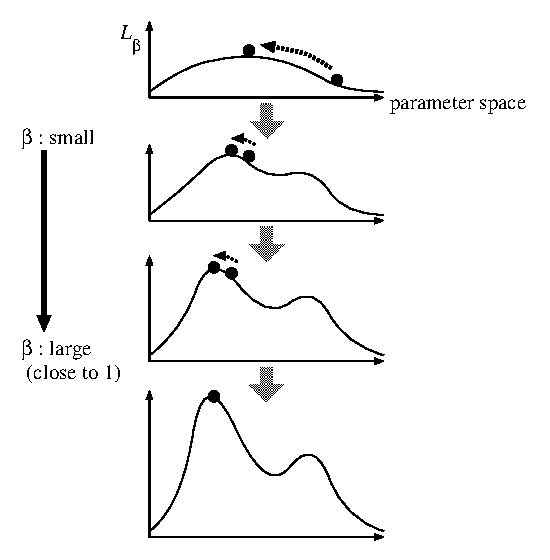
\includegraphics[scale=0.8]{fig/daem.eps}
}
\caption{Image of the deterministic annealing EM algorithm.}
\label{fig:daem}
\end{figure}

Another solution for avoiding undesirable local maxima is to use
the deterministic annealing EM (DAEM)\conindex{deterministic annealing EM algorithm}
\conindex{expectation-maximization algorithm!deterministic annealing ---|see{deterministic annealing EM algorithm}}
\conindex{DAEM algorithm|see{deterministic annealing EM algorithm}}
algorithm~\cite{Ueda98}.  It is easy to see that, in the usual EM algorithm,
the final estimate of the parameters depends on the choice of initial parameters.
On the other hand, the DAEM algorithm is designed to reduce an undesirable
influence from the initial parameters in the early stage of EM iterations.
In the rest of this section, we briefly describe the DAEM algorithm.

Let us consider first that we have the observed data (a multiset of observed goals)
$D=\{G_1,G_2,\ldots,G_T\}$, and $\psi(G_t)$ is the set of explanations
for the $t$-th observed goal.  Then, from analogy to statistical mechanics,
the free energy\conindex{free energy!--- in statistical mechanics} is introduced as:
\begin{equation}
\mathcal{F}_\beta=-\frac{1}{\beta}\sum_{t=1}^T\log\sum_{E\in\psi(G_t)} P_\theta(E)^\beta,
\end{equation}
where $\beta$ is the {\em inverse temperature}\conindex{inverse temperature}
which controls the influence from the initial parameters. The DAEM algorithm
is derived so that it tries to minimize the free energy $\mathcal{F}_\beta$ at
each temperature $1/\beta$.  Figure~\ref{fig:daem} shows an
expected behavior of the DAEM algorithm, where $L_\beta$ is introduced
as $-\mathcal{F}_\beta$ (then we will try to maximize $L_\beta$).
In the DAEM algorithm, we start
from the small $\beta$, under which $L_\beta$ is expected to
have a smooth shape, and hopefully has only one local maximum\conindex{local maximum}
(i.e.\ the global maximum).  So under the smaller $\beta$, we may be able to
find the global maximum or good local maxima.  When $\beta$ increases,
on the other hand, the shape of $L_\beta$ changes (becomes sharper),
and hence we should continue to update the parameters by EM iterations.
Please note that the starting point of these EM iterations is expected
to be more promising than the initial parameters.  Finally we perform
EM iterations at $\beta = 1$, which is equivalent to the usual EM iterations.

For an effective use of the DAEM algorithm, the annealing schedule
\conindex{annealing schedule} is
important. In PRISM, following \cite{Ueda98}, we start from $\beta_0=\beta_\mathrm{init}$
and then update $\beta$ by the update rule $\beta_{t+1}\leftarrow\beta_t\cdot\beta_\mathrm{rate}$,
where $\beta_\mathrm{init}$ and $\beta_\mathrm{rate}$ are given by the user
(the default values are 0.1 and 1.5, respectively).  In our experience,
the appropriate annealing schedule seems to vary depending on the model
and the observed data.

The DAEM algorithm will be enabled when the {\tt daem}\flagindex{daem} flag
is set as `{\tt on}', and controlled by the {\tt itemp\_init} and the
{\tt itemp\_rate} flags which correspond to $\beta_\mathrm{init}$
(the initial value)\conindex{inverse temperature!initial value of ---}
and $\beta_\mathrm{rate}$ (the increasing rate),
\conindex{inverse temperature!increasing rate of ---}
respectively.  For example, the followings will enable the DAEM algorithm
with $\beta_\mathrm{init}=0.3$ and $\beta_\mathrm{rate}=1.2$.
\begin{quote}
\begin{verbatim}
?- set_prism_flag(daem,on).
?- set_prism_flag(itemp_init,0.3).
?- set_prism_flag(itemp_rate,1.2).
\end{verbatim}
\end{quote}

While the DAEM algorithm running, the programming system displays an asterisk
(`{\tt *}') in the line beginning with `{\tt \#em-iters}' at the moment the
inverse temperature\conindex{inverse temperature} is updated.  For example,
in the HMM program, we will see the messages as follows:
%
\exindex{HMM program}
\flagindex{daem}
\flagindex{itemp\_init}
\flagindex{itemp\_rate}
\begin{quote}
\begin{small}
\begin{verbatim}
?- prism(hmm).
  :
?- set_prism_flag(daem,on).
  :
?- set_prism_flag(itemp_init,0.3).
  :
?- set_prism_flag(itemp_rate,1.2).
  :
?- hmm_learn(100).

#goals: 0.........(92)
Exporting switch information to the EM routine ... done
#em-iters: *0*****.**(13) (Converged: -687.729389314)
Statistics on learning:
        Graph size: 5420
        Number of switches: 5
        Number of switch instances: 10
        Number of iterations: 13
        Final log likelihood: -687.729389314
        Total learning time: 0.032 seconds
        Explanation search time: 0.008 seconds
        Total table space used: 369180 bytes
Type show_sw or show_sw_b to show the probability distributions.

yes
\end{verbatim}
\end{small}
\end{quote}
%
On the other hand, when the {\tt show\_itemp}\flagindex{show\_itemp} flag
(\secref{sec:built-in:flags:list}) turned `{\tt on}', the system will display
`{\tt <$\beta_t$>}' ($t=0,1,\ldots$) instead of asterisks.

\begin{table}[t]
\caption{Available statistics on the explanation graphs, on learning,
and on the probabilistic inference other than learning}
\label{tab:learn-stat}
\begin{center}
\begin{small}
\begin{tabular}{|l|l|}
\hline
\multicolumn{2}{|c|}{\tt graph\_statistics({\it Name},{\it Stat})}\\
\hline
\multicolumn{1}{|c|}{\it Name}&\multicolumn{1}{|c|}{\it Stat}\\
\hline
{\tt num\_subgraphs}\statindex{num\_subgraphs}&Number of subgraphs in the explanation graphs\conindex{explanation graph}\\
{\tt num\_nodes}\statindex{num\_nodes}&Total number of nodes in the explanation graphs\\
&\q(the sum of {\tt num\_goal\_nodes} and {\tt num\_switch\_nodes})\\
{\tt num\_goal\_nodes}\statindex{num\_goal\_nodes}&Number of subgoal nodes\\
{\tt num\_switch\_nodes}\statindex{num\_switch\_nodes}&Number of switch nodes\\
{\tt avg\_shared}\statindex{avg\_shared}
  &Average number of nodes which share a particular node (note: this average value\\
  &can be misleading if there is a node which is shared by extremely many nodes)\\
\hline
\multicolumn{2}{|c|}{\tt learn\_statistics({\it Name},{\it Stat})}\\
\hline
\multicolumn{1}{|c|}{\it Name}&\multicolumn{1}{|c|}{\it Stat}\\
\hline
{\tt log\_likelihood}\statindex{log\_likelihood}&Log likelihood\conindex{likelihood} (only available in ML/MAP)\\
{\tt log\_post}\statindex{log\_post}&Log of unnormalized a posteriori probability (in MAP)\conindex{a posteriori probability!unnormalized ---}\\
{\tt log\_prior}\statindex{log\_prior}&Log of a priori probability (in MAP)\conindex{prior probability}\\
{\tt lambda}\statindex{lambda}&Same as {\tt log\_likelihood} (in ML) or {\tt log\_post} (in MAP)\\
{\tt num\_switches}\statindex{num\_switches}&Number of occurred switches in the last learning\\
{\tt num\_switch\_values}\statindex{num\_switch\_values}&Number of occurred switch values in the last learning\\
{\tt num\_parameters}\statindex{num\_parameters}&Number of free parameters in the last learning\\
{\tt num\_iterations}\statindex{num\_iterations}&Number of EM/VT iterations in the last learning\\
{\tt goals}\statindex{goals}&List of goals used in the last learning\\
{\tt goal\_counts}\statindex{goal\_counts}&List of goal-count pairs\conindex{goal-count pair} used in the last learning\\
{\tt bic}\statindex{bic}&Bayesian Information Criterion\conindex{Bayesian Information Criterion} (in ML/MAP, see \secref{sec:built-in:learn:score})\\
{\tt cs}\statindex{cs}&Cheeseman-Stutz score\conindex{Cheeseman-Stutz score} (in MAP, see \secref{sec:built-in:learn:score})\\
{\tt free\_energy}\statindex{free\_energy}&Variational free energy\conindex{variational free energy} (in VB, see \secref{sec:vb:bg})\\
{\tt learn\_time}\statindex{learn\_time}&Total time consumed by the built-in (in seconds, including miscellaneous jobs)\\
{\tt learn\_search\_time}\statindex{learn\_search\_time}&Time consumed by the explanation search (in seconds)\\
{\tt em\_time}\statindex{em\_time}&Time consumed by the EM/VT algorithm (in seconds)\\
\hline
\multicolumn{2}{|c|}{\tt infer\_statistics({\it Name},{\it Stat})}\\
\hline
\multicolumn{1}{|c|}{\it Name}&\multicolumn{1}{|c|}{\it Stat}\\
\hline
{\tt infer\_time}\statindex{infer\_time}&Total time consumed by the built-in (in seconds, including miscellaneous jobs)\\
{\tt infer\_search\_time}\statindex{infer\_search\_time}&Time consumed by the explanation search (in seconds)\\
{\tt infer\_calc\_time}\statindex{infer\_calc\_time}&Time consumed by the numerical calculation (in seconds)\\
\hline
\multicolumn{2}{|c|}{\tt mcmc\_statistics({\it Name},{\it Stat})}\\
\hline
\multicolumn{1}{|c|}{\it Name}&\multicolumn{1}{|c|}{\it Stat}\\
\hline
{\tt mcmc\_sample\_time}\statindex{mcmc\_sample\_time}&Total time consumed by MCMC sampling (in seconds, including miscellaneous jobs)\\
{\tt mcmc\_marg\_time}\statindex{mcmc\_marg\_time}&Time consumed for the estimated log marginal liklihood\conindex{the estimated log marginal liklihood} (in seconds)\\
{\tt mcmc\_pred\_time}\statindex{mcmc\_pred\_time}&Time consumed for Viterbi explanation based on the MCMC samples (in seconds)\\
{\tt mcmc\_exact\_time}\statindex{mcmc\_exact\_time}&Time consumed for the exact log marginal likelihood\conindex{the estimated log marginal liklihood} (in seconds)\\
\hline
\end{tabular}
\end{small}
\end{center}
\end{table}

\section{Getting statistics on probabilistic inferences}
\label{sec:built-in:stat}

The built-in predicates
{\tt graph\_\lb statistics/0},\predindex{graph\_statistics/0}
{\tt learn\_\lb statistics/0},\predindex{learn\_statistics/0}
{\tt infer\_\lb statistics/0}\predindex{infer\_statistics/0}
and {\tt mcmc\_\lb statistics/0}\predindex{mcmc\_statistics/0} display
the statistics on the explanation graphs, on learning, on
the probabilistic inferences other than learning and on
MCMC sampling.  Besides,
{\tt prism\_\lb statistics/0}\predindex{prism\_statistics/0}
displays all statistics displayed by the above four built-ins.  
To get an individual statistic, we can respectively use
{\tt graph\_\lb statistics({\it Name},\lb {\it Stat})},
\predindex{graph\_statistics/2}
{\tt learn\_\lb statistics({\it Name},\lb {\it Stat})},
\predindex{learn\_statistics/2}
{\tt infer\_\lb statistics({\it Name},\lb {\it Stat})},
\predindex{infer\_statistics/2}
{\tt mcmc\_\lb statistics({\it Name},\lb {\it Stat})},
\predindex{mcmc\_statistics/2}
and {\tt prism\_\lb statistics({\it Name},\lb {\it Stat})},
\predindex{prism\_statistics/2}
where {\it Name} is the name of a statistic and {\it Stat} is
the value of the statistic.  For example, to get the time consumed
by learning, we may run:
\predindex{prism\_statistics/2}
\begin{quote}
\begin{small}
\begin{verbatim}
?- prism_statistics(learn_time,T).
\end{verbatim}
\end{small}
\end{quote}
When calling {\tt prism\_\lb statistics({\it Name},{\it Stat})}
\predindex{prism\_statistics/2}
with {\it Name} being unbound, we can get all available statistics
one after another by backtracking (this behavior also applies to
the built-ins {\tt graph\_\lb statistics/2}, {\tt learn\_\lb statistics/2}
and {\tt infer\_\lb statistics/2}). The available statistics are
shown in Table~\ref{tab:learn-stat}.\footnote{
The number of occurred switch instances
is just the sum of the numbers of possible outcomes of switches
occurred in all explanations for all observed goals.
This means that the switch instances not occurring in any of these
explanations are also taken into account there.
The number of free parameters is just computed as
the number of occurred switch instances subtracted by the number of
occurred switches.
}
Combining these statistics with
the facilities for saving/restoring switch information
(\secref{sec:built-in:switch:save_sw}), it is possible to a customized
routine for multiple runs of the EM algorithm\conindex{restart}
(\secref{sec:built-in:learn:restart}).

In addition, the observed goals\conindex{observed goal}
(with their counts and frequencies) used in the last
learning is displayed by {\tt show\_\lb goals}\predindex{show\_goals/0},
and can be obtained as Prolog terms by
{\tt get\_\lb goals/1}\predindex{get\_goals/1} and
{\tt get\_\lb goal\_\lb counts/1}\predindex{get\_goal\_counts/1}:
\conindex{goal-count pair}

\exindex{direction program}
\predindex{show\_goals/0}
\predindex{get\_goals/1}
\predindex{get\_goal\_counts/1}
\begin{quote}
\begin{small}
\begin{verbatim}
?- show_goals.
Goal direction(right) (count=1, freq=33.333%)
Goal direction(left) (count=2, freq=66.667%)
Total_count=3

?- get_goals(Gs).
Gs = [direction(left),direction(right)] ?

?- get_goal_counts(GCs).
GCs = [[direction(left),2,66.666666666666657],
       [direction(right),1,33.333333333333329]] ?
\end{verbatim}
\end{small}
\end{quote}


\section{Model scoring*}
\label{sec:built-in:learn:score}

In practical applications, we often face a problem of
{\em model selection}\conindex{model selection} --- that is, we need
to select the model that fits best the data at hand, from possible
candidates.  Since version 1.10, the programming system provides the
following Bayesian scores:\conindex{Bayesian score}
\begin{enumerate}
\item {\em Bayesian Information Criterion} (BIC)~\cite{Schwarz78},
  \conindex{Bayesian Information Criterion}
  \conindex{BIC|see{Bayesian Information Criterion}}
\item The {\em Cheeseman-Stutz (CS) score}~\cite{Cheeseman95},
  \conindex{Cheeseman-Stutz score}
  \conindex{CS score|see{Cheeseman-Stutz score}}
\item The {\em variational (negative) free energy},
  \conindex{variational free energy}
\item The {\em estimated log marginal likelihood}.
  \conindex{estimated log marginal likelihood}
\end{enumerate}
The first two are used after ML (\secref{sec:built-in:learn:mle}) or MAP
(\secref{sec:built-in:learn:mape}) estimation, whereas the third one is
used after variational Bayesian learning (Chapter~\ref{chap:vb})
and the last one is used after MCMC sampling (Chapter~\ref{chap:mcmc}).
Generally speaking, the first three Bayesian scores are known to
be `deterministic' approximations of $\log P(\data\mid M)$,
log of the {\em marginal likelihood}
\conindex{marginal likelihood} of the observed data $\data$ under the model $M$,
and so in model selection with some Bayesian score (BIC, for example),
we compare the model candidates according to the score (i.e.\ the model
with the larger score is considered to be better).
On the other hand, since version 2.1, the programming system provides
built-in predicates for MCMC sampling, by which we can obtain a sample-based
approximation of log of the marginal likelihood
(see Chapter~\secref{chap:mcmc} for details).

To be more concrete, let us consider first that the joint
distribution $P(\data,M,\theta)$ of the observed data $\data$, a probabilistic
model $M$, and its parameters $\theta$.  In PRISM, $\data$ is a multiset
of observed goals $G_1,G_2,\ldots,G_T$, and $M$ corresponds to
the modeling part\conindex{modeling part} of a PRISM program.
$P(\data,M,\theta)$ is then factored as
$P(\data\mid M,\theta)P(\theta\mid M)P(M)$ by the chain rule, where
$P(M)$ is the {\em prior distribution}\conindex{prior distribution}
of the model $M$, $P(\theta\mid M)$ is the {\em a posteriori distribution}
\conindex{a posteriori probability}\conindex{a posteriori distribution}
of the parameters $\theta$ of the model $M$, and $P(\data\mid M,\theta)$
is the {\em likelihood}\conindex{likelihood} of the data $\data$ based
on the model $M$ with the parameters $\theta$.  Then, in model selection,
our goal is to find the most probable model $M^\ast$ based on the data
$\data$ at hand, that is, we attempt to find $M^\ast$ such that:
\[
M^\ast
=\mathrm{argmax}_M\; P(M\mid\data)
=\mathrm{argmax}_M\; \frac{P(\data\mid M)P(M)}{P(\data)}
=\mathrm{argmax}_M\; P(\data\mid M),
\]
where we assume $P(M)$ to be uniform for simplicity.  Now the goal
is reduced to finding $M\;(=M^\ast)$ that maximizes $P(\data\mid M)$.
$P(\data\mid M)$ is commonly called the {\em marginal likelihood}
\conindex{marginal likelihood} of $\data$ given $M$, and is used as a
Bayesian score for model selection.  The marginal likelihood can be
interpreted as the expectation (or the average) of the likelihood
$P(\data\mid M,\theta)$ with respect to the prior distribution
$P(\theta\mid M)$\footnote{
As described in \secref{sec:built-in:learn:mape}, the programming system
assumes the prior distribution $P(\theta\mid M)$
($M$ was omitted in  for simplicity)
follows a Dirichlet distribution
$P(\theta\mid M)=\frac{1}{Z}\prod_{i,v}\theta_{i,v}^{\alpha_{i,v}-1}$,
where $Z$ is a normalizing constant and each $\alpha_{i,v}$ is a hyperparameter
of the Dirichlet distribution, which corresponds to {\tt msw($i$,$v$)}.
}:
\[
P(\data\mid M)
=\textstyle \int_{\Theta} P(\data,\theta\mid M) d\theta
=\textstyle \int_{\Theta} P(\data\mid M,\theta)P(\theta\mid M) d\theta
=\langle P(\data\mid M,\theta)\rangle_{P(\theta\mid M)}~.
\]

If the observed data were complete data $\data_c$, where each element in
$\data_c$ is a pair $(G_t,E_t)$ of the $t$-th goal $G_t$ and its
{\em unique} explanation $E_t$,
then $P(\data_c\mid M)$ is obtained in closed form
(see \cite{Cooper92} for the case with a Bayesian network\conindex{Bayesian network}).
On the other hand, when the observed data is incomplete, as in the case with
mixture models, the integral in the above equation is difficult to compute.
As mentioned above, BIC\conindex{Bayesian Information Criterion}
and the CS score\conindex{Cheeseman-Stutz score} are the approximations of
log of the marginal likelihood,\conindex{marginal likelihood} which are defined as:
\begin{eqnarray*}
\mathit{Score}_{\mathrm{BIC}}(M)
&\defined&\log P(\data\mid M,\hat{\theta}_{\mathrm{MAP}})-\frac{|\theta|}{2}\log N\\
\mathit{Score}_{\mathrm{CS}}(M)
&\defined&\log P(\tilde{\data}_c\mid M)- \log P(\tilde{\data}_c\mid M,\hat{\theta}_{\mathrm{MAP}})
+ \log P(\data\mid M,\hat{\theta}_{\mathrm{MAP}}),
\end{eqnarray*}
where $N$ is the total size of dataset, $|\theta|$ denotes the number
of free parameters, $\hat{\theta}_{\mathrm{MAP}}$ is the MAP estimate
of the parameters, and $\tilde{\data}_c$ is the pseudo complete data whose
sufficient statistics are the expected occurrences of random switches
obtained by the EM algorithm.  See \cite{Chickering97} for more detailed descriptions
about BIC and the CS score.  
In the programming system, {\tt learn\_\lb statistics(bic,\lb {\it Score})} or
{\tt learn\_\lb statistics(cs,\lb {\it Score})}\predindex{learn\_statistics/2}
(\secref{sec:built-in:stat})\conindex{statistics on probabilistic inferences}
will provide us BIC\conindex{Bayesian Information Criterion}
and the CS score\conindex{Cheeseman-Stutz score} after ML or
MAP learning (\secref{sec:built-in:learn:em-preds}) with
some observed goals $\data$.
The definitions of the variational free energy and another approximation
of the marginal likelihood via MCMC sampling will be shown in
Chapter~\ref{chap:vb} and Chapter~\ref{chap:mcmc}, respectively.

\section{Handling failures*}
\label{sec:built-in:failure}

The programming system provides a facility of dealing with failure
\conindex{failure (in the generation process)}
in generative models\conindex{generative model}.
The background and general descriptions are
given in \secref{sec:overview:failure} and \secref{sec:lang:model:failure},
and so in this section, we will concentrate on the usage of this facility.

For example, let us consider again the program which takes into
account the agreement in the results of coin-tossings, and suppose
that the program is contained in the file named `{\tt agree.psm}':

\exindex{agreement program}
\progindex{agree/1}
\begin{quote}
\begin{verbatim}
values(coin(_),[head,tail]).

failure :- not(success).
success :- agree(_).

agree(A):-
    msw(coin(a),A),
    msw(coin(b),B),
    A=B.
\end{verbatim}
\end{quote}
See \secref{sec:lang:model:failure} for a detailed reading of this program.
Like the program above, for the model that may cause failures, we need to
define the predicate {\tt failure/0}\predindex{failure/0}
which describes all generation processes\conindex{generation process}
leading to failure.  In a probabilistic context, the sum of probabilities
of successful generation processes and the probability that {\tt failure/0}
holds (called the {\em failure probability}\conindex{failure probability})
should always sum to unity.  Of course it is possible to define
{\tt failure/0} in a usual manner of PRISM programming, but the definition
should be much simpler if we can appropriately use the negation
{\tt not/1}\predindex{not/1} as above.

When some negation {\tt not/1} occurs in a program, the system first attempts
to eliminate it from  the program by applying a  certain type of program
transformation\conindex{program transformation}, called First Order
Compiler (FOC)~\cite{Sato89},\conindex{First Order Compiler}
\conindex{FOC|see{First Order Compiler}} to produce an ordinary
PRISM program.  If this transformation is successful, PRISM then loads the
transformed program into memory.\conindex{loading (the program)}
{\tt prismn({\it File})}\predindex{prismn/1} carries out this
two-staged process automatically (please note that `{\tt n}' is added to the last
of the predicate name).  {\it File} must include a definition of the
{\tt  failure/0} predicate described above.

By default, the transformed program is stored into the file `{\tt  temp}'
\commindex{temp} under the current working directory.  If you prefer another file,
say {\it TempFile}, {\tt prismn({\it File},{\it TempFile})}\predindex{prismn/2}
should be used instead.   For example, for the agreement program above, the query

\exindex{agreement program}
\predindex{prismn/1}
\begin{quote}
\begin{verbatim}
?- prismn(agree).
\end{verbatim}
\end{quote}

\noindent
loads `{\tt agree.psm}' into memory.  The user can check the result
of the transformation by FOC, looking at the file `{\tt  temp}'.  To estimate
the parameters of switches for this program, include a special symbol
{\tt failure}\index{predicate}{failure@{\tt failure} (Prolog atom used in {\tt learn/1})}
as data:

\exindex{agreement program}
\index{predicate}{failure@{\tt failure} (Prolog atom used in {\tt learn/1})}
\predindex{learn/1}
\progindex{agree/1}
\begin{quote}
\begin{verbatim}
?- learn([failure,agree(heads),agree(heads),agree(tails)]).
\end{verbatim}
\end{quote}

\noindent
For a batch execution (\secref{sec:system:batch})\conindex{batch execution}
of the program that deals with failures, we need to run a command
`{\tt upprism prismn:{\it foo}}' instead of `{\tt upprism {\it foo}}'.
\commindex{upprism}

{\tt foc/2}\predindex{foc/2} is the built-in predicate internally invoked
by {\tt prismn/1-2}\predindex{prismn/1}\predindex{prismn/2}.
That is, {\tt foc({\it File},{\it TempFile})} eliminates negation
(or more generally universally quantified implications)
and generates executable code into {\it TempFile}.  For example, we can
find the program `{\tt max}' under the `{\tt exs\_foc}' directory obtained
by extracting the package.  With the following query, we transform
`{\tt max}' into `{\tt temp}', and load the translated program:

\predindex{foc/2}
\begin{quote}
\begin{verbatim}
?- foc(max,temp),[temp].
\end{verbatim}
\end{quote}

\noindent
Allowing  negation\conindex{negation}  in  the  clause  body  is
equivalent  to allowing  arbitrary first-order formulas  as goals
which are obviously  impossible to  solve in  general.  So  {\tt foc/2}
may fail depending on  the source program.  Users are advised
to look into the examples of {\tt foc/2} usage under the `{\verb!foc!}'
directory.

It is unfortunate that the deterministic annealing EM (DAEM) algorithm
\conindex{deterministic annealing EM algorithm}
(\secref{sec:built-in:learn:daem}) does not work with the
failure-adjusted maximization (FAM) algorithm.\conindex{deterministic annealing EM algorithm}
This is because, under $\beta<1$ ($\beta$ is the inverse temperature
\conindex{inverse temperature} used in the DAEM algorithm),
the failure probability\conindex{failure probability} can exceed unity,
whereas the FAM algorithm is derived from the property of a
negative binomial distribution\conindex{negative binomial distribution}
under the condition that the failure probability is less than unity~\cite{Cussens01}.


\section{Avoiding underflow*}
\label{sec:built-in:underflow}
\conindex{underflow problem}

For large data, such as very long sequential data, we often suffer
from a problem that the probability of some explanation goes into underflow.
In version 2.0, the mechanism for avoiding underflow is simplified,
i.e. we just switch between logarithmic scale\conindex{logarithmic-scaled probability}
and non-logarithmic scale for the probabilities being kept in the programming system.
The default scale is non-logarithmic.

For Viterbi computation\conindex{Viterbi computation}
(\secref{sec:lang:inference} or \secref{sec:built-in:viterbi}),
the log-scaled probability of the Viterbi explanation\conindex{Viterbi probability}\conindex{Viterbi explanation}
is just computed as the sum of the log-scaled probabilities of
the switch instances in the explanation.
\conindex{Viterbi computation!log-scaled ---}
For the probabilistic inferences other than Viterbi computation,
the log-scaled probability computation\conindex{logarithmic-scaled probability}
is performed by calling the logarithmic function and the exponential function
alternately.  Although log-scaled probability computation is safe in most cases,
we should care about two points.  First, log-scaled probability computation
requires some additional computation time for the logarithmic function and
the exponential function.  The second point is that we often need to combine
the log-scaled probability computation with MAP estimation
(\secref{sec:built-in:learn:mape})\conindex{maximum a posteriori estimation}
to avoid a numerical problem that the programming system may take a logarithm
of zero probabilities.  With MAP estimation, on the other hand, we can
avoid having such zero probabilities.  If you do not prefer the side-effect
from MAP estimation, it is recommended to set very small pseudo counts
(e.g.\ $1.0\times 10^{-6}$).

To enable the log-scaled probability computation,\conindex{logarithmic-scaled probability}
please set `{\tt on}' to the {\tt log\_scale} flag\flagindex{log\_scale}
(the default value is {\tt off}).  Then the returned probability is
in logarithmic scale.  This setting is equivalent to simultaneously
setting `{\tt on}' to the {\tt log\_viterbi} flag
and `{\tt log\_exp}' to the {\tt scaling} flag in previous versions
of the programming system.
See \secref{sec:built-in:flags} for a general description on handling
execution flags.  


\section{Keeping the solution table*}\conindex{solution table}
\label{sec:built-in:table}

Since version 1.10, when the {\tt clean\_table}\flagindex{clean\_table}
flag is set as `{\tt off}' (see \secref{sec:built-in:flags}
for a general description on handling execution flags),
the programming system will come {\em not} to clean up the
solution table.\conindex{solution table}
On the other hand, if this flag is set as `{\tt on}', which is the default,
the programming system will automatically clean up
\conindex{solution table!automatic cleaning of ---} all past results of
explanation search\conindex{explanation search} (say, solutions)
in the solution table\footnote{
Internally, the system calls both {\tt initialize\_table/0}
\bpindex{initialize\_table/0}
(B-Prolog's built-in) and the routine that erases the ID tables
of PRISM's own.  So it is not guaranteed for the system to work
when you call only {\tt initialize\_table/0} at an arbitrary timing.
}
when invoking a routine that performs explanation
search\conindex{explanation search}, i.e.\ the routine for
probability calculation ({\tt prob/2} and its variants;
\secref{sec:built-in:prob}),
explanation graph construction ({\tt probf/2} and its variants;
\secref{sec:built-in:expl}), Viterbi computation
({\tt viterbif/2} and its variants; \secref{sec:built-in:viterbi}),
hindsight computation ({\tt hindsight/1} and its variants;
\secref{sec:built-in:hindsight}) and
learning ({\tt learn/0} and its variants; \secref{sec:built-in:learn}).

Keeping and reusing the past solutions can be significantly useful
when we compute the probabilities of some specific goal repeatedly
with different parameter settings.  Of course, the efficiency is gained
at the price of memory space, so we need to care about the size of
the used memory (i.e.\ the table area).
\conindex{table area}


\section{Execution flags}
\label{sec:built-in:flags}
\conindex{execution flag}

\subsection{Handling execution flags}
\label{sec:built-in:flags:handle}
\conindex{execution flag}

The programming system provides dozens of execution flags for allowing us
to change its behavior. The below is the usage of these execution flags:

\begin{description}
\item\underline{Setting flags}:

  The execution flags are set by the command
  {\tt set\_prism\_flag({\it FlagName},{\it Value})}.
  \predindex{set\_prism\_flag/2}
  There are a couple of typical usages:

  \begin{itemize}
  \item{\em At loading time}:

    The execution flags can be specified by the loading command
    {\tt prism/2} (\secref{sec:system:load}):
    \begin{quote}
      {\tt ?- prism([{\it FlagName}={\it Value}],{\it Filename}).}
    \end{quote}
    The programming systems will then behave under the setting
    {\tt {\it FlagName}={\it Value}}.

  \item{\em At the query prompt}:

    We can of course interactively set the execution flags at the query prompt:
    \begin{quote}
      {\tt ?- set\_prism\_flag({\it FlagName},{\it Value})}.
    \end{quote}
    The programming systems will then behave under the setting
    {\tt {\it FlagName}={\it Value}}.

  \item{\em In the query statements in the program}:

    When writing {\tt set\_prism\_flag/2} in some query statements in a program,
    these queries will be evaluated while loading.  They can be thought of as
    the default flag settings for the program.   Here is an example:
    \predindex{set\_prism\_flag/2}
\begin{quote}
\begin{verbatim}
    :
:- set_prism_flag(default_sw_d,1.0).
:- set_prism_flag(log_scale,on).
    :
\end{verbatim}
\end{quote}

  \item{\em In a batch routine}:

    It is often convenient to write {\tt set\_prism\_flag/2} in a batch predicate
    like {\tt go/1} shown below:
\predindex{set\_prism\_flag/2}
\begin{quote}
\begin{verbatim}
go(R) :-  % R is the number of random restarts
   set_prism_flag(restart,R),
   learn.
\end{verbatim}
\end{quote}
   Then, we can run ``{\tt ?- go({\it R})}'' with various {\it R}.

  \end{itemize}

\item\underline{Printing flags}:

  {\tt show\_prism\_flags/0}\predindex{show\_prism\_flags/0} or more shortly
  {\tt show\_flags/0} prints the current values of flags.

\item\underline{Getting flag values}:

  By {\tt get\_prism\_flag({\it FlagName},X)}, we can get the current
  value of {\it FlagName} as {\tt X}.\predindex{get\_prism\_flag/2}
  If we call this with {\it FlagName} being unbound, all available
  flags and their values are retrieved one after another by backtracking.

\item\underline{Resetting flags}:

  {\tt reset\_prism\_flags/0}\predindex{reset\_prism\_flags/0}
  resets all flags to their default values.

\end{description}

\subsection{Available execution flags}
\label{sec:built-in:flags:list}

Here we list the available execution flags in the alphabetical order.
Please note that this list also includes ones for the functions described
in later chapters.

\begin{itemize}
\item
  {\tt clean\_table}
  \flagindex{clean\_table}
  (possible values:\ {\tt on} and {\tt off}; default:\ {\tt on})
  --- the flag for automatic cleaning of the solution table
  (see \secref{sec:built-in:table} for details).
  \conindex{solution table!automatic cleaning of ---}
  If this flag is set as `{\tt on}', the programming system will
  automatically clean up all past solutions in the solution table
  when invoking any routine that executes the explanation
  search.\conindex{explanation search}
  On the other hand, with this flag turned `{\tt off}', we can keep
  the past solutions.
\item{\tt crf\_enable}
  \flagindex{crf\_enable}
  (possible values:\ {\tt on}, {\tt off}, default:\ {\tt on})
  --- this flag enables the use of built-in predicates for generative CRFs
  (\secref{chap:crf}).
\item{\tt crf\_golden\_b}
  \flagindex{crf\_golden\_b}
  (possible value:\ non-negative float, default:\ 1.0)
  --- this flag  sets a parameter used in golden section line search
  in learning generative CRFs (\secref{chap:crf}).  Search is done
  between 0 and the value set by the flag.
\item{\tt crf\_init}
  \flagindex{crf\_init}
  (possible values: {\tt none}, {\tt noisy\_u}, {\tt random} and {\tt zero}, default:\ {\tt zero})
  --- this  flag specifies how  to initialize the weights $\vlambda$  in learning
  generative CRFs (\secref{chap:crf}).
  There are  four options: {\tt none},  {\tt noisy\_u}, {\tt  random} and {\tt zero}.
  {\tt zero} means initialization to 0.
\item{\tt crf\_learn\_mode}
  \flagindex{crf\_learn\_mode}
  (possible values:\ {\tt fg} and {\tt lbfgs}, default:\ {\tt lbfgs})
  --- the {\tt crf\_learn\_mode} flag specifies a learning mode,  either {\tt fg}
  or {\tt lbfgs}, for generative CRFs (\secref{chap:crf}).
  The {\tt fg}  mode applies the steepest descent method for
  minimization which is a line  search method.  Starting from an initial value
  $\vlambda_0$,  the weights $\vlambda_{n}$ are iteratively updated at step $n$ by
  \begin{eqnarray*}
    \vlambda_{n+1} & = & \vlambda_{n} + \alpha_n \vd_n \\
    \vd_n & = & \nabla{\cal L}(\vlambda_n \mid D),
  \end{eqnarray*}
  where $\alpha_n$, learning  rate, is controlled by the {\tt crf\_learn\_rate} flag.
  %
  The {\tt lbfgs} mode uses L-BFGS,\conindex{L-BFGS algorithm}
  a  powerful quasi-Newton  method, to
  minimize  $-{\cal L}(\vlambda  \mid  D)$.  Usually  L-BFGS converges  more
  quickly than  the steepest descent  method.  However the convergence  may be
  sensitive to initialization and as an alternative the steepest descent method
  is offered.
\item{\tt crf\_learn\_rate}
  \flagindex{crf\_learning\_rate}
  (possible values:\ {\tt backtrack} and {\tt golden}, default: {\tt backtrack})
  --- this flag controls a learning  rate $\alpha_n$ when
  the {\tt crf\_learn\_mode} flag is set to {\tt fg},
  the steepest descent algorithm.\conindex{steepest descent algorithm}
  $\alpha_n$ is determined by line search:\ 
  $\alpha_n = \argmin_\alpha {\cal L}(\vlambda_n + \alpha \vd_n \mid D)$.
  If the {\tt crf\_learn\_mode} flag is set to {\tt backtrack},
  backtracking line search is used to perform ${\rm argmin}_\alpha$.
  Likewise {\tt golden} performs golden section line search.
\item{\tt crf\_ls\_c1}
  \flagindex{crf\_ls\_c1}
  (possible value:\ floating-point number in $[0, 1]$, default: 0.5)
  --- this flag sets another parameter used in backtracking line search
  in learning generative CRFs (\secref{chap:crf}).
\item{\tt crf\_ls\_rho}
  \flagindex{crf\_ls\_rho}
  (possible value:\ floating-point number in $[0, 1]$, default: 0.5)
  --- this flag sets a parameter used in backtracking line search
  in learning generative CRFs (\secref{chap:crf}).
\item{\tt crf\_penalty}
  \flagindex{crf\_penalty}
  (possible value:\ any floating-point number, default:\ 0.0)
  --- this flag determines $\mu$ in the penalty term\conindex{penalty term}
  $\frac{\mu}{2}\sum_{k=1}^{K}\lambda_k^2$ in learning generative CRFs (\secref{chap:crf}).
  \conindex{generative conditional random fields}
\item{\tt sgd\_penalty}
\flagindex{sgd\_penalty}
(possible value:\ any floating-point number, default:\ 0.01)
--- this flag determines a coefficient of the $L_2$ penalty term, for learning to rank (\secref{chap:rank}).
\item{\tt sgd\_learning\_rate}
\flagindex{sgd\_learning\_rate}
(possible value:\ any floating-point number, default:\ 0.01)
--- this flag determines the learning rate (or its initial value when the adaptive method is used) of stochastic gradient decent, for learning to rank (\secref{chap:rank}).
\item{\tt sgd\_optimizer}
\flagindex{sgd\_optimizer}
(possible values:\ {\tt sgd}, {\tt adadeleta} and {\tt adam}, default:\ {\tt adam})
--- the {sgd\_optimizer} flag specifies the algorithm to optimize the learning rate, for learning to rank  (\secref{chap:rank}).
\item
  {\tt daem}
  \flagindex{daem}
  (possible values:\ {\tt on} and {\tt off}; default:\ {\tt off})
  --- the flag for enabling the deterministic annealing EM (DAEM) algorithm
  \conindex{deterministic annealing EM algorithm}
  (see \secref{sec:built-in:learn:daem}).  If this flag is
  set as `{\tt on}', the programming system will invoke the DAEM
  algorithm while EM learning.  On the other hand, with this flag
  turned `{\tt off}', it will be disabled.
\item
  {\tt data\_source}
  \flagindex{data\_source}
  (possible values:\ {\tt data/1}, {\tt file({\it Filename})}, {\tt none};
  default:\ {\tt data/1})
  ---
  the data file for {\tt learn/0} (\secref{sec:built-in:learn:em-preds}).
  If this flag is set as {\tt data/1}, the observed goals are read from the
  file specified by the data file declaration\conindex{data file declaration}
  (\secref{sec:lang:decl:data}) as in the versions earlier than 1.12.
  If {\tt file({\it Filename})}, the observed goals are read from {\it Filename}.
  If {\tt none}, the programming system assumes that there is no data file
  available for {\tt learn/0} and thus raises an error when {\tt learn/0} is
  called.  By setting {\tt file({\it Filename})} or {\tt none}, you can use
  {\tt data/1} as a user predicate for the purposes other than
  data file declaration.
\item
  {\tt default\_sw}
  \flagindex{default\_sw}
  (possible values:\ {\tt none}, {\tt uniform}, {\tt f\_\lb geometric},
  {\tt f\_\lb geometric({\it Base})},\\
  {\tt f\_\lb geometric({\it Base}, \lb {\it Type})}, and
  {\tt random}; default:\ {\tt uniform})
  ---
  the default distribution for parameters.
  \conindex{switch!default distribution of a ---}
  If {\tt none} is set, we have no default distribution for parameters,
  and hence as in the versions earlier than 1.9, we cannot make sampling
  or probability computation without an explicit parameter setting
  (via {\tt set\_sw/2}, and so on) or learning. {\tt uniform} means
  that the default distribution for each switch is a uniform distribution.
  \conindex{uniform distribution}
  {\tt f\_geometric(\lb {\it Base}, {\it Type})} means the default distribution
  for each switch is a finite geometric distribution
  \conindex{finite geometric distribution}
  where {\it Base} is its base (a floating-point number greater than one)
  and {\it Type} is {\tt asc} (ascending order) or {\tt desc} (descending order).
  For example, when the flag is set as {\tt f\_geometric(2,asc)},
  the parameters of some three-valued switch are set to 0.142$\cdots$
  ($= 2^0/(2^0+2^1+2^2)$), 0.285$\cdots$ ($= 2^1/(2^0+2^1+2^2)$),
  and 0.574$\cdots$ ($= 2^2/(2^0+2^1+2^2)$), according to the order of values
  specified in the corresponding multi-valued switch declaration ({\tt values/2-3}).
  {\tt f\_geometric({\it Base})} is the same as
  {\tt f\_geometric({\it Base},desc)},
  and {\tt f\_geometric} is the same as {\tt f\_geometric(2,desc)}.
  {\tt random} means that the default distribution for each switch is set
  at random.
\item
  {\tt default\_sw\_a}
  \flagindex{default\_sw\_a}
  (possible values:\ {\tt none}, {\tt uniform}, {\tt uniform($\zeta$)}, $\zeta$
  ($\zeta$ is a positive float); 
  default:\ {\em disabled} --- see below)
  ---
  the default value for pseudo counts (hyperparameters) $\alpha_{i,v}$ used
  in variational Bayesian learning.\conindex{pseudo count}
  \conindex{switch!default pseudo counts of a ---}
  If {\tt none} is set, we have no default distribution for pseudo counts,
  and hence we cannot perform probabilistic inferences unless giving the
  pseudo counts, by {\tt set\_sw\_a/2} or variational Bayesian
  learning (\secref{sec:vb:built-in:em}, \secref{sec:vb:built-in:vt}).
  {\tt uniform} (resp.\ {\tt uniform($\zeta$)}) means that each pseudo count will
  be set as $1/K$ (resp.\ $\zeta/K$) by default, where $K$ is the number
  of possible values of the corresponding switch.
  If a positive floating-point number $\zeta$ is set to
  this flag, the system use $\zeta$ as the default value of each pseudo count.
  This flag will be disabled if the {\tt default\_sw\_d} flag is set
  to some value.  This flag is {\em disabled} just after the programming system
  invoked.
\item
  {\tt default\_sw\_d}
  \flagindex{default\_sw\_d}
  (possible values:\ {\tt none}, {\tt uniform}, {\tt uniform($\zeta$)}, $\zeta$
  ($\zeta$ is a non-negative float); 
  default:\ 0.0)
  ---
  the default value for pseudo counts $\delta_{i,v}$ used in
  MAP estimation.\conindex{pseudo count}
  \conindex{switch!default pseudo counts of a ---}
  If {\tt none} is set, we have no default distribution for pseudo counts,
  and hence we cannot perform probabilistic inferences unless giving the
  pseudo counts by {\tt set\_sw\_d/2} (or variational Bayesian learning).
  {\tt uniform} (resp.\ {\tt uniform($\zeta$)}) means that each pseudo count will
  be set as $1/K$ (resp.\ $\zeta/K$) by default, where $K$ is the number
  of possible values of the corresponding switch.
  If a non-negative floating-point number $\zeta$ is set to
  this flag, the system use $\zeta$ as the default value of each pseudo count.
  This flag will be disabled if the {\tt default\_sw\_a} flag is set
  to some value.  This flag is {\em enabled} just after the programming system
  invoked.
\item
  {\tt em\_progress}
  \flagindex{em\_progress}
  (possible value:\ positive integer; default:\ {\tt 10})
  ---
  the frequency of printing the progress message (i.e.\ the dot symbol)
  in the EM algorithm
  (\secref{sec:built-in:learn:mle})\conindex{expectation-maximization algorithm}.
\item
  {\tt epsilon}
  \flagindex{epsilon}
  (possible value:\ non-negative float; default:\ {\tt 1.0e-4})
  --- the threshold $\varepsilon$ for judging convergence in the EM algorithm
  \conindex{expectation-maximization algorithm!convergence of ---}
  (see \secref{sec:built-in:learn:mle}).
\item
  {\tt error\_on\_cycle}
  \flagindex{error\_on\_cycle}
  (possible values:\ {\tt on} and {\tt off}; default:\ {\tt on})
  ---
  the flag for checking cycles in the calling relationship.
  By default or when this flag is set as `{\tt on}', the
  programming system checks the existence of a cycle in the calling
  relationship, and if any cycle exists, the system will stop
  immediately.  When this flag is set as `{\tt off}', the system does
  {\em not} check such acyclicity and we are able to obtain an
  explanation graph that violates the acyclicity condition.
  \conindex{acyclicity condition}
  Of course this flag is very experimental and seems not to be used
  in usual cases.
\item
  {\tt explicit\_empty\_expls}
  \flagindex{explicit\_empty\_expls}
  (possible values:\ {\tt on} and {\tt off}; default:\ {\tt on})
  ---
  The built-in predicate {\tt probf/2}\predindex{probf/2}
  (\secref{sec:built-in:expl}) outputs an explanation graph
  which is a list of Prolog terms taking the form {\tt node($G$,{\it Es})}
  where $G$ is a subgoal and {\it Es} is a list of $G$'s explanations.
  If $G$ is known to be always true, {\it Es} is bound to {\tt [path([],[])]}
  since version 2.0.  On the other hand, when setting {\tt off} to
  this flag, {\it Es} will be bound to {\tt []} as done in the earlier
  versions.
\item
  {\tt fix\_init\_order}
  \flagindex{fix\_init\_order}
  (possible values:\ {\tt on} and {\tt off}; default:\ {\tt on})
  ---
  the flag for fixing the order of parameter initialization among switches.
  For an implementational reason, in the EM algorithm
  (\secref{sec:built-in:learn:mle}),
  the order of parameter initialization among switches can vary according
  to the platform, and hence we may have different learning results among
  the various platforms.
  Turning this flag `{\tt on}' fixes the initialization order
  in some manner, and will yield the same learning result.
\item
  {\tt force\_gc}
  \flagindex{force\_gc}
  (possible values:\ {\tt on} and {\tt off}; default:\ {\tt on})
  ---
  the flag for performing garbage collection\conindex{garbage collection}
  after the every call of the built-ins {\tt probf/1-2} (and their variants),
  {\tt viterbif/\{1,3\}}, {\tt hindsight/2-3} and {\tt chindsight/2-3}.
  This flag is just experimental.
  For the stability of the programming system, this flag is activated
  by default, but if you have a sufficient space for control stack and
  heap,\conindex{control stack + heap} garbage collection could be skipped.
\item
  {\tt init}
  \flagindex{init}
  (possible values:\ {\tt none}, {\tt random} and {\tt noisy\_u};
  default:\ {\tt random})
  ---
  the initialization method in the EM algorithm
  (\secref{sec:built-in:learn:mle}).
  \conindex{expectation-maximization algorithm}
  {\tt none} means no initialization, {\tt random} means that the parameters
  are initialized almost at random, and {\tt noisy\_u} means that the
  parameters are initialized to be uniform with (small) Gaussian noises.
  The variance of Gaussian noises can be changed by the {\tt std\_ratio}
  \flagindex{std\_ratio} flag.
\item
  {\tt itemp\_init}
  \flagindex{itemp\_init}
  (possible value:\ floating-point number $b$ such that $0<b\le 1$; default:\ {\tt 0.1})
  ---
  the initial value $\beta_\mathrm{init}$ of
  the inverse temperature\conindex{inverse temperature} $\beta$ used
  in the deterministic annealing EM (DAEM) algorithm (\secref{sec:built-in:learn:daem}).
  \conindex{deterministic annealing EM algorithm}
\item
  {\tt itemp\_rate}
  \flagindex{itemp\_rate}
  (possible value:\ floating-point number $b$ such that $b>1$; default:\ {\tt 1.5})
  ---
  the increasing rate $\beta_\mathrm{rate}$ of
  the inverse temperature\conindex{inverse temperature} $\beta$ used
  in the DAEM algorithm (\secref{sec:built-in:learn:daem}).
  \conindex{deterministic annealing EM algorithm}
\item
  {\tt learn\_message}
  \flagindex{learn\_message}
  (possible values:\ see below; default:\ {\tt all})
  ---
  the flag for controlling the messages being displayed while EM learning is conducted
  (by {\tt learn/0-1}; \secref{sec:built-in:learn}).  Currently, there are four
  types of messages:
  \begin{enumerate}
  \item The message on the progress of explanation search
  \item The message on the progress of the EM algorithm (the numeric part)
  \item The message on the summary statistics
  \item Some other miscellaneous messages
  \end{enumerate}
  These messages are enabled by giving {\tt search}, {\tt em}, {\tt stats} and
  {\tt misc}, respectively, to this flag.  We can specify the combination of
  these flag values by concatenating with `{\tt +}'.  For example, if the value
  {\tt search+em} is given, {\tt learn/0-1} will only show the messages on the
  progress of explanation search and EM learning.  In addition, {\tt all} is an
  abbreviation of {\tt search+em+stats+misc}, and if {\tt none} is given,
  {\tt learn/0-1} will show no message.  By default, all types of messages
  will be displayed similarly to the earlier versions.
\item
  {\tt learn\_mode}
  \flagindex{learn\_mode}
  (possible values:\ {\tt ml}, {\tt vb}, {\tt both}, {\tt ml\_vt},
  {\tt vb\_vt} and {\tt both\_vt}; default:\ {\tt ml})
  ---
  the underlying statistical framework for parameter learning.
  The values {\tt ml}, {\tt vb} and {\tt both} are related to EM learning.
  If this flag is set as `{\tt ml}', the system will conduct the EM algorithm
  for ML/MAP estimation\conindex{maximum likelihood estimation}
  \conindex{maximum a posteriori estimation}
  (\secref{sec:built-in:learn:em}), by which we can get point-estimated
  parameters\conindex{parameter} of random switches.
  If this flag is set as `{\tt vb}', the system
  will conduct VB-EM algorithm\conindex{variational Bayesian EM algorithm}
  (\secref{sec:vb:built-in:em}),
  by which we can get adjusted pseudo counts\conindex{pseudo count}
  (or equivalently, the hyperparameters\conindex{hyperparameter})
  of switches.  With `{\tt both}', we can get both point-estimated parameters
  and adjusted hyperparameters by EM learning.
  The remaining values {\tt ml\_vt}, {\tt vb\_vt} and {\tt both\_vt}
  are related to Viterbi training.
  If this flag is set as `{\tt ml\_vt}', the system will conduct
  Viterbi training in the ML/MAP setting
  (\secref{sec:built-in:learn:vt}), by which we can get point-estimated
  parameters of random switches.
  If this flag is set as `{\tt vb\_vt}', the system
  will conduct VB-VT algorithm\conindex{variational Bayesian VT algorithm}
  (\secref{sec:vb:built-in:vt}),
  by which we can get adjusted pseudo counts\conindex{pseudo count}
  (or equivalently, the hyperparameters\conindex{hyperparameter})
  of switches.  With `{\tt both\_vt}',
  we can get both point-estimated parameters and adjusted hyperparameters
  by Viterbi training.
\item
  {\tt log\_scale}
  \flagindex{log\_scale}
  (possible values:\ {\tt on} and {\tt off}; default:\ {\tt off})
  ---
  the flag for enabling/disabling the log-scaled probability computation
  (\secref{sec:built-in:underflow}).\conindex{logarithmic-scaled probability}
  For large data, we often suffer from the problem that the probability of
  some explanation goes into underflow.\conindex{underflow problem}
  By turning this flag on (setting `{\tt on}' to this flag), we can avoid
  this problem by using the log-scaled probabilities.
  This is equivalent to simultaneously setting `{\tt on}'
  to the {\tt log\_viterbi} flag and `{\tt log\_exp}' to the {\tt scaling}
  flag in the previous versions of the programming system.
  In learning, it is highly recommended to combine log-scaled probability
  computation with MAP estimation (see \secref{sec:built-in:underflow}).
\item
  {\tt max\_iterate}
  \flagindex{max\_iterate}
  (possible value:\ positive integer, {\tt default} and {\tt inf}; default:\ {\tt default})
  ---
  the maximum number of EM iterations to be performed.  In the EM algorithm
  (\secref{sec:built-in:learn:mle}),
  \conindex{expectation-maximization algorithm}
  sometimes we need a large number of iterations until convergence.
  \conindex{expectation-maximization algorithm!convergence of ---}
  For such a case, we can stop the EM algorithm before convergence
  by this flag.  
  `{\tt default}' means that the maximum number of iterations
  is the system's default value (10000, in the current version).
  With `{\tt inf}', the system do not put any limit on the number
  of iterations.
\item
  {\tt mcmc\_b}
  \flagindex{mcmc\_b}
  (possible value:\ non-negative integer, default:\ 1000)
  ---
  the length of so-called `burn-in' period\conindex{burn-in period}
  in MCMC sampling ($\Hburn$ in \secref{sec:mcmc:bg:sample}).
\item
  {\tt mcmc\_e}
  \flagindex{mcmc\_e}
  (possible value:\ non-negative integer, default:\ 2000)
  ---
  the length of the Markov chain in MCMC sampling
  ($H$ in \secref{sec:mcmc:bg:sample}).
\item
  {\tt mcmc\_message}
  \flagindex{mcmc\_message}
  (possible values:\ see below; default:\ {\tt all})
  ---
  the flag controlling the messages being displayed while MCMC sampling is conducted
  by {\tt mcmc/1-2}\predindex{mcmc/1-2} (\secref{sec:mcmc:built-in:primitive}).
  Note that this flag cannot be applied to the `batch' predicates related
  to MCMC sampling (i.e.\ the built-ins in
  \secref{sec:mcmc:built-in:marg} and \secref{sec:mcmc:built-in:viterbi}).
  Currently, there are five types of messages:
  \begin{enumerate}
  \item The message on the progress of explanation search
  \item The message on the progress of the VB-EM algorithm (the numeric part)
  \item The message on the progress of MCMC sampling
  \item The message on the summary statistics
  \item Some other miscellaneous messages
  \end{enumerate}
  See \secref{sec:mcmc:bg:sample} for the entire procedure of MCMC sampling.
  These messages are enabled by giving {\tt search}, {\tt em}, {\tt mcmc},
  {\tt stats} and {\tt misc}, respectively, to this flag.  We can specify the
  combination of these flag values by concatenating with `{\tt +}'.  For example,
  if the value {\tt em+mcmc} is given, {\tt mcmc/1-2} will only show the messages
  on the progress of the VB-EM algorithm and MCMC sampling.  In addition,
  {\tt all} is an abbreviation of {\tt search+em+mcmc+stats+misc},
  and if {\tt none} is given, {\tt mcmc/1-2} will show no message.
  By default, all types of messages will be displayed.
\item
  {\tt mcmc\_progress}
  \flagindex{mcmc\_progress}
  (possible value:\ positive integer, default:\ 100)
  ---
  the frequency of printing the progress message (i.e.\ the dot symbol)
  in MCMC sampling (\secref{sec:mcmc:bg:sample}).
\item
  {\tt mcmc\_s}
  \flagindex{mcmc\_s}
  (possible value:\ positive integer, default:\ 5)
  ---
  the length of the cycle of picking up a sample in MCMC sampling
  ($\Hskip$ in \secref{sec:mcmc:bg:sample}).
%% \item
%%   {\tt reduce\_copy}
%%   \flagindex{reduce\_copy}
%%   (possible values:\ {\tt on} and {\tt off}; default:\ {\tt off})
%%   ---
%%   the flag for automatic copying of the Prolog terms returned by several
%%   built-ins ({\tt probf/2}\predindex{probf/2},
%%   {\tt viterbif/3}\predindex{viterbif/3}, and so on;
%%   See \secref{sec:built-in:problem}).
%%   If this flag is set as `{\tt off}', the programming system will
%%   automatically make a copy of the Prolog term returned by these built-ins.
%%   On the other hand, with this flag turned `{\tt on}', such a copying
%%   will be skipped.
\item
  {\tt rerank}
  \flagindex{rerank}
  (possible value:\ positive integer; default:\ {\tt 10})
  ---
  the number of intermediate candidates in reranking\conindex{reranking}
  for the Viterbi computation based on the hyperparameters
  (\secref{sec:vb:built-in:viterbi}).
\item
  {\tt reset\_hparams}
  \flagindex{reset\_hparams}
  (possible values:\ {\tt on} and {\tt off}; default:\ {\tt on})
  ---
  the flag on resetting of the pseudo counts\conindex{pseudo count} (hyperparameters)
  in the repeated runs of VB-EM algorithm
  \conindex{variational Bayesian EM algorithm!repeated runs of ---}
  (\secref{sec:vb:built-in:em})
  and VB-VT algorithm
  \conindex{variational Bayesian Viterbi training algorithm!repeated runs of ---}
  (\secref{sec:vb:built-in:vt}).
  By default or if this flag is set as `{\tt on}', the programming system will
  reset the pseudo counts with the default values (internally, it calls
  {\tt set\_sw\_all\_a/0}; \secref{sec:built-in:switch:set_sw}) in advance of
  these learning algorithms.  If this flag is set as `{\tt off}', on the other hand,
  it can be observed that the pseudo counts monotonically increases as we repeatedly
  run VB learning (this behavior might be common in Bayesian learning). 
\item
  {\tt restart}
  \flagindex{restart}
  (possible value:\ positive integer; default:\ {\tt 1})
  ---
  the number of restarts
  (\secref{sec:built-in:learn:restart}).\conindex{restart}
  Generally speaking, the EM algorithm\conindex{expectation-maximization algorithm}
  (\secref{sec:built-in:learn:mle})
  only finds a local ML/MAP estimate\conindex{local maximum},
  so we often restart the EM algorithm for several
  times with different initial parameters, and get the best parameters
  (i.e.\ with the highest log-likelihood or log of a posteriori probability)
  among these restarts.
  This flag is also applicable to VB-EM algorithm (\secref{sec:vb:built-in:em})
  and VB-VT algorithm (\secref{sec:vb:built-in:vt}).
\item
  {\tt search\_progress}
  \flagindex{search\_progress}
  (possible value:\ non-negative integer; default:\ {\tt 10})
  ---
  the frequency of printing the progress message (i.e.\ the dot symbol)
  in explanation search\conindex{explanation search}
  and in constructing explanation graphs\conindex{explanation graph}.
  if 0 is set, the progress message will be suppressed.
\item
  {\tt show\_itemp}
  \flagindex{show\_itemp}
  (possible values:\ {\tt on} and {\tt off}; default:\ {\tt off})
  ---
  the flag for showing the inverse temperature\conindex{inverse temperature} in the DAEM algorithm (\secref{sec:built-in:learn:daem}).
  If this flag is set as `{\tt on}', the programming system displays the inverse temperature like `{\tt <0.100>}' each time it is updated.
  Otherwise, each update is indicated by an asterisk (`{\tt *}').
\item
  {\tt sort\_hindsight}
  \flagindex{sort\_hindsight}
  (possible values:\ {\tt by\_goal} and {\tt by\_prob}; default:\ {\tt by\_goal})
  ---
  the flag for the mode on sorting the results of hindsight computation
  \conindex{hindsight computation}
  (\secref{sec:built-in:hindsight}).
  With {\tt by\_goal}, the result will be sorted in the Prolog's
  standard order with respect to the subgoals.  With {\tt by\_prob},
  the result will be ordered by the magnitude of the hindsight probability.
  \conindex{hindsight probability}
\item
  {\tt std\_ratio}
  \flagindex{std\_ratio}
  (possible value:\ non-negative float; default:\ {\tt 0.2})
  ---
  the control parameter for the variance of Gaussian noises used in
  initialization of switch parameters in the EM algorithm
  \conindex{expectation-maximization algorithm}
  (\secref{sec:built-in:learn:mle};
  see also the description on the {\tt init}\flagindex{init} flag).
  When we initialize parameters  with a $k$-valued switch according
  to a uniform distribution with Gaussian noises from
  $N(1/k,(\mbox{\tt std\_ratio}/k)^2)$.
  The parameters will be normalized at the end of initialization.
  Note that this flag works differently in VB-learning
  (see \secref{sec:vb:built-in:init} for details).
\item
  {\tt verb}
  \flagindex{verb}
  (possible values:\ {\tt none}, {\tt graph}, {\tt em} and {\tt full}; default:\ {\tt none})
  ---
  the flag for extra messages in EM learning (\secref{sec:built-in:learn:mle}).
  `{\tt none}' means that no extra message will be displayed.
  If this flag is set as `{\tt graph}', the explanation graphs\conindex{explanation graph}
  will be displayed after the explanation search.  By `{\tt em}', we can get
  the more detailed information about the EM algorithm.
  \conindex{expectation-maximization algorithm}  If `{\tt full}' is set, we will see
  both the explanation graphs and the information about EM.
\item
  {\tt viterbi\_mode}
  \flagindex{viterbi\_mode}
  (possible values:\ {\tt ml} and {\tt vb}; default:\ {\tt ml})
  ---
  the underlying statistical framework for Viterbi computation.
  If this flag is set as `{\tt ml}', the system will conduct the Viterbi
  computation based on the current parameter values (\secref{sec:built-in:viterbi}).
  If `{\tt vb}' is set, on the other hand, the system
  will conduct the Viterbi computation for VB learning based on the current
  hyperparameters (\secref{sec:vb:built-in:viterbi}).
\item
  {\tt warn}
  \flagindex{warn}
  (possible values:\ {\tt on} and {\tt off}; default:\ {\tt off})
  ---
  the flag for enabling/disabling warning messages.\conindex{warning message}
\item
  {\tt write\_call\_events}
  \flagindex{write\_call\_events}
  (possible values:\ Prolog atoms representing events (\secref{sec:system:debug:write_call}), {\tt none} and {\tt off}; default:\ {\tt all})
  ---
  the default events at which the execution messages are displayed by {\tt write\_\lb call/1-2}%
  \predindex{write\_call/1}\predindex{write\_call/2}.
  If this flag is set as {\tt none}, the message is not displayed unless
  some events are specified in the options of {\tt write\_call/2}.
  If this flag is set as {\tt off}, the message will not be displayed
  regardless of the options passed to {\tt write\_call/2}.
%% 2.3
\item{{\tt rank\_loss}}
\flagindex{rank\_loss}
(possible values:\ {\tt hinge}, {\tt square}, {\tt exp} and {\tt log}, default:\ {\tt hinge})
--- this flag specifies the pairwise loss function (\secref{rank}) for learning to rank (Chapter~\ref{chap:rank}).

\item{{\tt rank\_loss\_c}}
\flagindex{rank\_loss\_c}
(possible value:\ any floating-point number, default:\ 1)
--- this flag determines a parameter $c$ in  Eq.~\ref{eq:rank_loss_h} and \ref{eq:rank_loss_sq} for learning to rank (Chapter~\ref{chap:rank}).

\item{{\tt sgd\_adam\_beta}}
\flagindex{\tt sgd\_adam\_beta}
(possible value:\ any floating-point number, default:\ 0.9)
--- this flag determines a parameter $beta$ in Eq.~\ref{eq:adam} of Adam for learning to rank (Chapter~\ref{chap:rank}).

\item{{\tt sgd\_adam\_epsilon}}
\flagindex{\tt sgd\_adam\_epsilon}
(possible value:\ any floating-point number, default:\ 1.0e-08)
--- this flag determines a parameter $epsilon$ in Eq.~\ref{eq:adam} of Adam for learning to rank (Chapter~\ref{chap:rank}).

\item{{\tt sgd\_adam\_gamma}}
\flagindex{\tt sgd\_adam\_gamma}
(possible value:\ any floating-point number, default:\ 0.999)
--- this flag determines the parameter $gamma$ in Eq.~\ref{eq:adam} of Adam for learning to rank (Chapter~\ref{chap:rank}).


\item{{\tt sgd\_adadelta\_epsilon}}
\flagindex{\tt sgd\_adadelta\_epsilon}
(possible value:\ any floating-point number, default:\ 1.0e-08)
--- this flag determines the parameter $epsilon$ in Eq.~\ref{eq:adadelta} of Adadelta for learning to rank (Chapter~\ref{chap:rank}).

\item{{\tt sgd\_adadelta\_gamma}}
\flagindex{\tt sgd\_adadelta\_gamma}
(possible value:\ any floating-point number, default:\ 0.95)
--- this flag determines the parameter $gamma$ in Eq.~\ref{eq:adadelta} of Adadelta learning rate for learning to rank (Chapter~\ref{chap:rank}).

\item{{\tt sgd\_learning\_rate}}
\flagindex{sgd\_learning\_rate}
(possible value:\ any floating-point number, default:\ 0.0001)
--- this flag determines the learning rate (or its parameter when adaptive methods are used) of stochastic gradient decent for learning to rank (Chapter~\ref{chap:rank}).

\item{{\tt sgd\_optimizer}}
\flagindex{sgd\_optimizer}
(possible values:\ {\tt sgd}, {\tt adadeleta} and {\tt adam}, default:\ {\tt adam})
--- the {sgd\_optimizer} flag specifies the algorithm to optimize the learning rate, for learning to rank  (Chapter~\ref{chap:rank}).

\item{{\tt sgd\_penalty}}
\flagindex{sgd\_penalty}
(possible value:\ any floating-point number, default:\ 0.01)
--- this flag determines the coefficient of the $L_2$ penalty for learning to rank (Chapter~\ref{chap:rank}).

\item{{\tt num\_minibatch}}
\flagindex{num\_minibatch}
(possible value:\ any positive integer, default:\ 1)
--- this flag determines the number of minibatch in learning to rank (Chapter~\ref{chap:rank}). The size of minibatch (the number of samples in a minibatch) is automatically determined by equally dividing the data.
Because the default value is one, the data is not divided into minibatches by default.
Note that the loss function does not always decrease while optimizing parameters when the number of minibatches is greater than one; therefore, this system does not notify rising the loss as an error.
When the specified {\tt num\_minibatch} is greater than the number of data,
{\tt num\_minibatch} is set as the number of data.
%%
\end{itemize}


\section{Random routines}
\label{sec:built-in:random}

The programming system contains an implementation of the {\em Mersenne Twister}
(\url{http://www.math.sci.hiroshima-u.ac.jp/~m-mat/MT/emt.html})\conindex{Mersenne Twister}
for a random number generator.  This generator is internally used in sampling
(\secref{sec:built-in:sample}) and the initialization step of parameter learning
(\secref{sec:built-in:learn}), and can be accessed by the built-in predicates
described in this section.  These built-in predicates have the names beginning
with `{\tt random\_}'.

\subsection{Configuring the random number generator}
\label{sec:built-in:random:config}

In a pseudo random number generator, including Mersenne Twister, the sequence of
generated random numbers is solely determined by the random seed\conindex{random seed}
with which the generator is initialized.  To enable us to control the sequence,
the programming system provides a couple of built-ins for getting and setting
the random seed:
\begin{itemize}
\item {\tt random\_get\_seed({\it Seed})}\predindex{random\_get\_seed/1}
returns the random seed set by the most recent call to {\tt random\_\lb set\_\lb seed/0-1}.
\item {\tt random\_set\_seed}\predindex{random\_set\_seed/0} \noargs
initializes the generator with a seed determined according to the current system time.
This predicate is called by the programming system during its start-up.
\item {\tt random\_set\_seed({\it Seed})}\predindex{random\_set\_seed/1}
initializes the generator with {\it Seed}.
\end{itemize}
There are also built-ins to save and restore the internal state of the generator,
with which we can reproduce the sequence from an arbitrary point:
\begin{itemize}
\item {\tt random\_get\_state({\it State})}
returns the present internal state of the generator as a ground term {\it State}.
This term can be stored into files and dynamic predicates.
\item {\tt random\_set\_state({\it State})}
restores the internal state of the generator to {\it State}.
The argument should be a term obtained by {\tt random\_get\_state/1}.
\end{itemize}

\subsection{Random numbers}
\label{sec:built-in:random:number}

Here is the list of built-ins for generating random numbers:
\begin{itemize}
\item {\tt random\_int({\it Max},{\it N})}\predindex{random\_int/2}
returns a random integer {\it N} such that $0 \le N < {\it Max}$.
\item {\tt random\_int({\it Min},{\it Max},{\it N})}\predindex{random\_int/3}
returns a random integer {\it N} such that ${\it Min} \le N  <  {\it Max}$.
\item {\tt random\_int\_incl({\it Min},{\it Max},{\it N})}\predindex{random\_int\_incl/3}
returns a random integer {\it N} such that ${\it Min} \le N \le {\it Max}$.
\item {\tt random\_int\_excl({\it Min},{\it Max},{\it N})}\predindex{random\_int\_excl/3}
returns a random integer {\it N} such that ${\it Min}  <  N  <  {\it Max}$.
\item {\tt random\_uniform({\it X})}\predindex{random\_uniform/1}
returns a random floating-point number {\it X} in $[0,1)$ under the uniform distribution.
\item {\tt random\_uniform({\it Max},{\it X})}\predindex{random\_uniform/2}
returns a random floating-point number {\it X} in $[0,{\it Max})$ under the uniform distribution.
\item {\tt random\_uniform({\it Min},{\it Max},{\it X})}\predindex{random\_uniform/3}
returns a random floating-point number {\it X} in $[{\it Min},{\it Max})$ under the
uniform distribution.
\item {\tt random\_gaussian({\it X})}\predindex{random\_gaussian/1}
returns a random floating-point number {\it X} under a normal distribution with the mean 0
and the standard deviation 1.
\item {\tt random\_gaussian({\it Mu},{\it Sigma},{\it X})}\predindex{random\_gaussian/3}
returns a random floating-point number {\it X} under a normal distribution with the mean
{\it Mu} and the standard deviation {\it Sigma}.
\end{itemize}

\subsection{Model-independent random choices}
\label{sec:built-in:random:choice}

It is possible to make random choices by sampling on random switches ({\tt msw/2}).
However, this way is sometimes inconvenient, in particular when the choices are not
a part of the model.  That is, we should give the outcome spaces and the distributions
to random switches (by {\tt set\_sw/2}) in advance.  To provide a quick way for random choices,
the programming system provides the following built-in predicates:%
\begin{itemize}
\item {\tt random\_select({\it Values},{\it V})}\predindex{random\_select/2}
chooses {\it V} randomly from {\it Values} according to the uniform distribution.
\item {\tt random\_select({\it Values},{\it Dist},{\it V})}\predindex{random\_select/3}
chooses {\it V} randomly from {\it Values} according to the distribution {\it Dist}.
\end{itemize}
{\it Values} and {\it Dist} should be specified in the same manner as {\tt values/2-3}
(\secref{sec:lang:decl:msw}) and {\tt set\_sw/2} (\secref{sec:built-in:switch:set_sw})
respectively, optionally with extended forms (e.g.\@ `{\tt [1-20,25-50@5]}';
see \secref{sec:built-in:switch:term})
and/or distribution forms (e.g.\@ `{\tt uniform}', `{\tt f\_geometric}', and so on;
also see \secref{sec:built-in:switch:term}).
Note that {\tt random\_\lb select/2} always follows the uniform distribution, not the
distribution indicated by the flag {\tt default\_\lb sw} (\secref{sec:built-in:flags:list}).

For example, using {\tt random\_select/3} as shown below, we may sample the phenotypes
of blood types according to the distribution $P_{\mathrm{A}}=0.4$, $P_{\mathrm{B}}=0.2$,
$P_{\mathrm{O}}=0.3$ and $P_{\mathrm{AB}}=0.1$:
\begin{quote}
\begin{small}
\begin{verbatim}
?- random_select([a,b,o,ab],[0.4,0.2,0.3,0.1],X).
X = a ?

?- random_select([a,b,o,ab],[0.4,0.2,0.3,0.1],X).
X = o ?

?- random_select([a,b,o,ab],[0.4,0.2,0.3,0.1],X).
X = b ?
\end{verbatim}
\end{small}
\end{quote}

\subsection{Advanced random routines}
\label{sec:built-in:random:advanced}

In addition to those mentioned in the previous subsections, the following built-in predicates
are provided as more advanced random routines:
\begin{itemize}
\item {\tt random\_multiselect({\it List},{\it N},{\it Output})}\predindex{random\_multiselect/3}
simultaneously chooses {\it N} elements from {\it List} uniformly at random.
\item {\tt random\_group({\it List},{\it N},{\it Output})}\predindex{random\_group/3}
randomly divides all elements in {\it List} into {\it N} groups.
{\it Output} is a (nested) list of {\it N} groups, where each group is represented by
a list of elements belonging to that group.
\item {\tt random\_shuffle({\it List},{\it Output})}\predindex{random\_shuffle/2}
randomly reorders the elements in {\it List}.
\end{itemize}
Here are a couple of usage examples:
\begin{quote}
%%  Seed = 152573659
\begin{small}
\begin{verbatim}
?- random_multiselect([1,2,3,4,5,6,7,8,9,10],3,Out).
Out = [1,5,6] ?

?- random_group([1,2,3,4,5,6,7,8,9,10],3,Out).
Out = [[4,5],[1,2,6,8],[3,7,9,10]] ?

?- random_shuffle([1,2,3,4,5,6,7,8,9,10],Out).
Out = [3,7,8,9,5,1,2,4,10,6] ?
\end{verbatim}
\end{small}
\end{quote}


\section{Statistical operations}
\label{sec:built-in:measure}

Dozens of built-in predicates are available for calculating statistical measures
(such as average and variance) of a given sequence of values, as listed in Table~\ref{tab:measure}.
Each predicate takes one input argument {\it List} for a list of values and one
output argument {\it Y} for the calculated statistical measure.  All values in
{\it List} are expected to be numeric except for the predicates returning the mode.

\begin{table}[t]
\caption{Available built-ins for statistical measures (see \secref{sec:built-in:measure} for notations)}
\label{tab:measure}
%%  macro available only in this environment
\def\RBP#1#2#3#4{{\tt #1({\it List},{\it Y})}\bpindex{#1/2}&{\tt #2}&#3&#4\\[0.25ex]}%
\def\Row#1#2#3#4{{\tt #1({\it List},{\it Y})}\predindex{#1/2}&{\tt #2}&#3&#4\\[0.25ex]}%
\def\Div{\mathbin{\big/}}%
\begin{center}
\begin{small}
\begin{tabular}{|l|l|l|l|}
\hline
\multicolumn{1}{|c|}{\em Predicate} &
\multicolumn{1}{|c|}{\em Op} &
\multicolumn{1}{|c|}{\em Description} &
\multicolumn{1}{|c|}{\em Formula} \\
\hline
\RBP{sumlist}{sum}{sum [B-Prolog's built-in]}
    {$\sum_i x_i$}
\Row{avglist}{avg}{average (arithmetic mean)\conindex{mean!arithmetic ---}}
    {$\bar{x} \equiv \sum_i x_i \Div n$}
\Row{meanlist}{mean}{average (arithmetic mean)\conindex{mean!arithmetic ---}}
    {$\bar{x} \equiv \sum_i x_i \Div n$}
\Row{gmeanlist}{gmean}{geometric mean\conindex{mean!geometric ---}}
    {$\left( \prod_i x_i \right)^{1/n}$}
\Row{hmeanlist}{hmean}{harmonic mean\conindex{mean!harmonic ---}}
    {$\left( \sum_i 1 / x_i \right)^{-1} \cdot n$}
\Row{varlistp}{varp}{variance\conindex{variance}}
    {$m_2 \equiv \sum_i ( x_i - \bar{x} )^2 \Div n$}
\Row{varlist}{var}{variance (estimator)\conindex{variance}}
    {$k_2 \equiv \sum_i ( x_i - \bar{x} )^2 \Div (n - 1)$}
\Row{stdlistp}{stdp}{standard deviation\conindex{standard deviation}}
    {$m_2^{1/2}$}
\Row{stdlist}{std}{standard deviation (estimator)\conindex{standard deviation}}
    {$k_2^{1/2}$}
\Row{semlistp}{semp}{standard error of the mean\conindex{standard error of the mean}}
    {$(m_2 / n)^{1/2}$}
\Row{semlist}{sem}{standard error of the mean (estimator)\conindex{standard error of the mean}}
    {$(k_2 / n)^{1/2}$}
\Row{skewlistp}{skewp}{skewness\conindex{skewness}}
    {$m_3 \Div m_2^{3/2}$}
\Row{skewlist}{skew}{skewness (estimator)\conindex{skewness}}
    {$k_3 \Div k_2^{3/2}$}
\Row{kurtlistp}{kurtp}{kurtosis\conindex{kurtosis}}
    {$\bigl( m_4 \Div m_2^2 \bigr) - 3$}
\Row{kurtlist}{kurt}{kurtosis (estimator)\conindex{kurtosis}}
    {$k_4 \Div k_2^2$}
\Row{modelist}{mode}{mode\conindex{mode} (see \secref{sec:built-in:measure})}
    {---}
\Row{amodelist}{amode}{mode\conindex{mode} (see \secref{sec:built-in:measure})}
    {---}
\Row{rmodelist}{rmode}{mode\conindex{mode} (see \secref{sec:built-in:measure})}
    {---}
\Row{pmodelist}{pmode}{probabilistic mode\conindex{mode!probabilistic ---} (see \secref{sec:built-in:measure})}
    {---}
\Row{medianlist}{median}{median\conindex{median}}
    {---}
\Row{minlist}{min}{minimum}
    {$\min \{x_i\}$}
\Row{maxlist}{max}{maximum}
    {$\max \{x_i\}$}
\RBP{length}{len}{length [B-Prolog's built-in]}
    {$n$}
\hline
\end{tabular}
\end{small}
\end{center}
\end{table}

In Table~\ref{tab:measure}, $n$ denotes the length of {\it List}; $x_i$ denotes the
$i$-th value in {\it List} ($1 \le i \le n$); $\bar{x}$ denotes the sample mean; $m_r$
denotes the $r$-th sample central moment; and $k_r$ denotes the $r$-th $k$-statistic
or the unique symmetric unbiased estimator of the $r$-th cumulant~\cite{MathWorld}.

There are four variants available for obtaining the mode as follows:
\begin{itemize}
  \item {\tt modelist({\it List},{\it Y})}
    returns a single value with the highest frequency.
    If multiple values have the highest frequency, this predicate returns the value
    coming first in the standard order.%
    \footnote{
      The {\em standard order} refers to the order defined by the comparison
      operator `{\tt @<}'.
    }
  \item {\tt amodelist({\it List},{\it Y})}
    returns a list containing all values with the highest frequency.
    The values in the resultant list are sorted by the standard order.
  \item {\tt rmodelist({\it List},{\it Y})}
    returns one of the values with the highest frequency.
    If multiple values have the highest frequency, this predicate chooses one of
    them randomly.
  \item {\tt pmodelist({\it List},{\it Y})}
    chooses one element according to the frequencies in {\it List}.%
    \footnote{
      Indeed, this has the same effect as {\tt random\_select/2}
      (\secref{sec:built-in:random:choice}) which just randomly chooses one element,
      although they are implemented separately.}
\end{itemize}

\noindent
In addition, the programming system provides the built-in
{\tt agglist({\it List},{\it Queries})}\predindex{agglist/2} that allows us to calculate two
or more statistical measures at once.  {\it Queries} is a list of queries each having the form
{\tt {\it Op}={\it Y}}, where {\it Op} is one of those listed in the column `{\it Op}' of
Table~\ref{tab:measure} and {\it Y} is unified with the cor\-re\-spond\-ing statistics.
For example:%
\footnote{
  The values do not look exact just because B-Prolog prints floating-point numbers
  with the precision more than they can retain.
}
\begin{quote}
\begin{small}
\begin{verbatim}
?- agglist([48,64,40,30,82],[mean=Avg,var=Var,std=Std]).
Var = 421.199999999999932
Avg = 52.799999999999997
Std = 20.523157651784484 ?
\end{verbatim}
\end{small}
\end{quote}


\section{List processing}
\label{sec:built-in:list}

The programming system provides several built-in predicates that implement
the map function\conindex{map function} in functional programming languages,
as well as the reduction operation.\conindex{reduction operation}%
\footnote{
  A function for reduction operations is called {\tt fold} in major
  functional programming languages, but the name {\tt reducelist} was chosen
  rather than {\tt foldlist} to avoid confusion with unfold/fold transformation
  of logic programs.
}
In addition, it is highly recommended to use the extended syntactic constructs
for `foreach'\conindex{foreach}\bpindex{foreach} and list comprehensions\conindex{list comprehension}
which are newly introduced in B-Prolog 7.4 (\url{http://www.probp.com/download/loops.pdf}).
These syntactic constructs are compiled at loading time, whereas the current
implementation of the {\tt maplist} predicates uses the assert/retract
utility for evaluation of the {\it Body} argument.
Here is a list of the built-in predicates:
\begin{itemize}
  \item {\tt maplist({\it X},{\it Body},{\it Xs})}\predindex{maplist/3}
    succeeds when {\it Xs} is a list, and {\it Body} succeeds for every element of {\it Xs}.
    {\it Body} is the body of a {\em deterministic} clause that takes one argument {\it X},
    which will be unified with each element from {\it Xs}.
  \item {\tt maplist({\it X},{\it Y},{\it Body},{\it Xs},{\it Ys})}\predindex{maplist/5}
    succeeds when {\it Xs} and {\it Ys} are lists of the same size, and {\it Body}
    succeeds for every pair of corresponding elements in {\it Xs} and {\it Ys}.
    {\it Body} is the body of a {\em deterministic} clause that takes two arguments
    {\it X} and {\it Y}, which will be unified with each pair from {\it Xs} and {\it Ys},
    respectively.
  \item {\tt maplist({\it X},{\it Y},{\it Z},{\it Body},{\it Xs},{\it Ys},{\it Zs})}\predindex{maplist/7}
    succeeds when {\it Xs}, {\it Ys} and {\it Zs} are lists of the same size, and {\it Body}
    succeeds for every triplet of corresponding elements in {\it Xs}, {\it Ys} and {\it Zs}.
    {\it Body} is the body of a {\em deterministic} clause that takes three arguments {\it X},
    {\it Y} and {\it Z}, which will be unified with each triplet from {\it Xs}, {\it Ys} and
    {\it Zs}, respectively.
  \item {\tt maplist\_func({\it F},{\it Xs})}\predindex{maplist\_func/2}
    succeeds when {\it Xs} is a list, and the predicate {\it F} succeeds for every element in
    {\it Xs}.  This is equivalent to {\tt maplist(X,{\it F}(X),{\it Xs})}.
  \item {\tt maplist\_func({\it F},{\it Xs},{\it Ys})}\predindex{maplist\_func/3}
    succeeds when {\it Xs} and {\it Ys} are the lists of the same size, and the predicate {\it F}
    succeeds for every pair of corresponding elements in {\it Xs} and {\it Ys}.
    This is equivalent to {\tt maplist(\lb X,\lb Y,\lb {\it F}(X,Y),\lb {\it Xs},\lb {\it Ys})}.
  \item {\tt maplist\_func({\it F},{\it Xs},{\it Ys},{\it Zs})}\predindex{maplist\_func/4}
    succeeds when {\it Xs}, {\it Ys} and {\it Zs} are the lists of the same size, and the predicate
    {\it F} succeeds for every triplet of corresponding elements in {\it Xs}, {\it Ys} and {\it Zs}.
    This is equivalent to {\tt maplist(X,Y,Z,{\it F}(X,Y,Z),{\it Xs},{\it Ys},{\it Zs})}.
  \item {\tt maplist\_math({\it Op},{\it Xs},{\it Ys})}\predindex{maplist\_math/3}
    constructs a list by applying an algebraic unary operator {\it Op} to each value in {\it Xs},
    and returns the resultant list to {\it Ys}.
    {\it Xs} must be a list containing only numerical values.
    This is equivalent to {\tt maplist(X,Y,(Y is {\it Op}(X)),{\it Xs},{\it Ys})}, but is more efficient.
  \item {\tt maplist\_math({\it Op},{\it Xs},{\it Ys},{\it Zs})}\predindex{maplist\_math/4}
    constructs a list by applying an algebraic binary operator {\it Op} to each pair of values
    in {\it Xs} and {\it Ys}, and returns the resultant list to {\it Zs}.
    {\it Xs} and {\it Ys} must be lists of the same size containing only numerical values.
    This is equivalent to {\tt maplist(X,Y,Z,(Z is {\it Op}(X,Y)),{\it Xs},{\it Ys},{\it Zs})},
    but is more efficient.
  \item {\tt reducelist($Y$,$X$,$Y'$,{\it Body},{\it List},{\it Init},{\it Value})}\predindex{reducelist/7}
    calls {\it Body} for each element of {\it List} to obtain {\it Value}, where {\it Body} is
    the body of a {\em deterministic} clause that takes three arguments $Y$, $X$ and $Y'$.
    Let {\tt p($Y$,$X$,$Y'$)} refer to the given clause and $X_i$ denote the $i$-th element of
    {\it List}, and then this predicate calls {\tt p($Y_{i-1}$,$X_i$,$Y_i$)} for $i=1,\ldots,n$ in turn,
    where $Y_0$ is given by {\it Init} and $n$ is the length of {\it List}, and returns $Y_n$ to {\it Value}.
  \item {\tt reducelist\_func({\it F},{\it List},{\it Init},{\it Value})}\predindex{reducelist\_func/4}
    calls the predicate {\it F} for each element of {\it List} to obtain {\it Value}.
    This is equivalent to {\tt reducelist(Y0,X,Y1,{\it F}(Y0,X,Y1),{\it List},{\it Init},{\it Value})}.
  \item {\tt reducelist\_math({\it Op},{\it List},{\it Init},{\it Value})}\predindex{reducelist\_math/4}
    applies an algebraic binary operator {\it Op} through the elements in {\it List} to obtain {\it Value}.
    {\it List} must consist only of numerical values.
    This is equivalent to {\tt reducelist(Y0,\lb X,\lb Y1,\lb (Y1 is {\it Op}(Y0,X)),\lb {\it List},\lb {\it Init},\lb {\it Value})},
    but is more efficient.
\end{itemize}
The following examples illustrate the usage of these predicates:
\begin{quote}
\begin{small}
\begin{verbatim}
?- maplist(X,Y,(Y is X-1),[1,2,3],Ys).
Ys = [0,1,2]

?- maplist(p(X),q(X),true,[p(x),p(y),p(z)],Ys).
Ys = [q(x),q(y),q(z)]

?- maplist(X,Y,atom_chars(X,Y),Xs,[[f,o,o],[t,r,u,e],[x]]).
Xs = [foo,true,x]

?- maplist(X,Y,Z,(Z is X*X+Y),[1,2,3],[10,20,30],Zs).
Zs = [11,24,39]

?- reducelist(Y0,X,Y1,(Y1 is Y0+2**X),[1,2,3],0,Out).
Out = 14

?- reducelist_func(append,[[2],[3,4],[5]],[0,1],Out)  
Out = [0,1,2,3,4,5]
\end{verbatim}
\end{small}
\end{quote}

\noindent
There are also the built-in predicates for list processing:
\begin{itemize}
  \item {\tt sublist({\it Sub},{\it List})}\predindex{sublist/2}
    succeeds when {\it Sub} is a sublist of {\it List}.
    This is inspired by \cite{Sterling86} and equivalent to
    {\tt sublist({\it Sub},{\it List},\_,\_)}, where {\tt sublist/4} is defined below.
  \item {\tt sublist({\it Sub},{\it List},{\it I},{\it J})}\predindex{sublist/4}
    succeeds when {\it Sub} is a list containing the $(I+1)$-th to the $J$-th elements
    (one-based indices are used here) in {\it List}.
    This predicate is backtrackable.
  \item {\tt splitlist({\it Prefix},{\it Rest},{\it List},{\it N})}\predindex{splitlist/4}
    succeeds when {\it Prefix} and {\it Rest} are lists, {\it List} is a concatenation of those lists, and
    {\it Prefix} has exactly {\it N} elements.  This predicate is backtrackable.
  \item {\tt grouplist({\it List},{\it K},{\it Sizes},{\it Output})}\predindex{grouplist/4}
    succeeds when the elements in {\it List} is divided into {\it K} groups according to {\it Sizes} and
    the result is represented by {\it Output}.  {\it Sizes} is a list of {\it K} elements in which the
    $i$-th element $N_i$ indicates the size of the $i$-th group.  {\it Output} is a nested list in which
    the $i$-th inner list corresponds to the $i$-th group and contains the $(M_{i-1}+1)$-th to the $M_i$-th
    elements in {\it List} where $M_0 = 0$ and $M_i = N_1+\cdots+N_i$ for $1 \le i \le K$.
    This predicate is backtrackable, but {\it K} must be instantiated.
  \item {\tt egrouplist({\it List},{\it K},{\it Output})}\predindex{egrouplist/3}
    divides the elements in {\it List} into {\it K} equal-sized groups.
    If the elements cannot be equally divided into the groups, the former groups will have the size larger by one than
    the latter groups.  {\it Output} is a nested list in which the $i$-th inner list corresponds to the $i$-th group
    formed in the same manner as {\tt grouplist/4}.  {\it List} and {\it K} must be instantiated,%
    \footnote{Note that the length of {\it List} is needed to determine the size of each group.}
    and thus this predicate is deterministic unlike {\tt grouplist/4}.
  \item {\tt countlist({\it Term},{\it List},{\it Count})}\predindex{countlist/3}
    counts the number of elements in {\it List} which are {\em variants} of {\it Term}, and returns the result to {\it Count}.
  \item {\tt countlist({\it List},{\it Counts})}\predindex{countlist/2}
    counts the occurrence for each variant appearing in {\it List}, and returns those occurrences as a list {\it Counts}.
    Each element in {\it Counts} has the form {\tt {\it Term}={\it Count}} and represents that variants of {\it Term}
    occurs {\it Count} times in {\it List}.
    The elements in {\it Counts} are ordered by decreasing order of {\it Count} then by the standard order of {\it Term}.
  \item {\tt filter({\it Patt},{\it Xs},{\it Ys})}\predindex{filter/3}
    leaves only the terms matching with {\it Patt} in the list {\it Xs}, and returns the resultant list to {\it Ys}.
    In the filtering predicates, a term {\it T} is considered to match with {\it Patt} if {\it T} is more
    specific than {\it Patt}, or more precisely {\it T} can be instantiated from {\it Patt}.%
    \footnote{
      This corresponds to the behavior of {\tt subsumes\_chk/2} available on some Prolog systems (e.g.\@ SWI-Prolog and XSB).
    }
    For example, the pattern {\tt f(a,\_,\_)} matches {\tt f(a,b,c)}, {\tt f(a,1,\_)}, {\tt f(a,X,g(X))}, {\tt f(a,\_,\_)},
    and so on, but does not {\tt f(a,b)}, {\tt f(a,b,c,d)}, {\tt f(x,y,z)}, {\tt g(a,b,c)}, {\tt f(\_,\_,\_)}, a variable,
    etc.
  \item {\tt filter({\it Patt},{\it Xs},{\it Ys},{\it Count})}\predindex{filter/4}
    leaves only the terms matching with {\it Patt} in the list {\it Xs}, and returns the resultant list to {\it Ys} and its length to {\it Count}.
  \item {\tt filter\_not({\it Patt},{\it Xs},{\it Ys})}\predindex{filter\_not/3}
    removes the terms matching with {\it Patt} from the list {\it Xs}, and returns the resultant list to {\it Ys}.
  \item {\tt filter\_not({\it Patt},{\it Xs},{\it Ys},{\it Count})}\predindex{filter\_not/4}
    removes the terms matching with {\it Patt} from the list {\it Xs}, and returns the resultant list to {\it Ys} and its length to {\it Count}.
  \item {\tt number\_sort({\it Xs},{\it Ys})}\predindex{number\_sort/2}
    sorts\conindex{sorting} the list {\it Xs} in numerically ascending order and returns the resultant list to {\it Ys}.
    This is equivalent to {\tt custom\_sort(A,B,(A<B),{\it Xs},{\it Ys})}, but much more efficient than {\tt custom\_sort/5}.
  \item {\tt custom\_sort({\it Cmp},{\it Xs},{\it Ys})}\predindex{custom\_sort/3}
    sorts\conindex{sorting} the list {\it Xs} according to the comparator {\it Cmp} and returns the resultant list to {\it Ys}.
    This is equivalent to {\tt custom\_sort(A,\lb B,\lb {\it Cmp}(A,B),\lb {\it Xs},\lb {\it Ys})}.
  \item {\tt custom\_sort({\it A},{\it B},{\it Body},{\it Xs},{\it Ys})}\predindex{custom\_sort/5}
    sorts\conindex{sorting} the list {\it Xs} according to the comparator {\it Body} and returns the resultant list to {\it Ys}.
    Here {\it Body} is a clause body that succeeds when {\it A} precedes {\it B}.
    {\it Body} should represent a total order for the values in {\it Xs}; otherwise the result would be unpredictable.
    The order among equal elements are preserved (i.e.\@ the sorting is {\em stable}).
\end{itemize}
Here are some examples:
\begin{quote}
\begin{small}
\begin{verbatim}
?- sublist(Sub,[a,b,c,d,e],2,4).
Sub = [c,d] ?

?- splitlist(List1,List2,[a,b,c,d,e,f],2).
List1 = [a,b]
List2 = [c,d,e,f] ?

?- grouplist([p,q,r,s,t,u,v,w],3,[4,2,2],Groups).
Groups = [[p,q,r,s],[t,u],[v,w]] ?

?- egrouplist([p,q,r,s,t,u,v,w],3,Groups).
Groups = [[p,q,r],[s,t,u],[v,w]] ?

?- countlist(a,[a,b,a,c,a,a,c,b,c],N).
N = 4 ?

?- countlist(f(_),[f(A),f(B),f(x),g(_),f(x),f(g(_)),_,f(_)],N).
N = 3 ?

?- countlist([a,b,a,c,a,a,c,b,c],Counts).
Counts = [a=4,c=3,b=2] ?

?- countlist([f(A),f(B),f(x),g(_),f(x),f(g(_)),_,f(_)],Counts).
Counts = [f(_c80)=3,f(x)=2,_c74=1,f(g(_c70))=1,g(_c8c)=1] ?

?- filter(f(_),[f(A),f(B),f(x),g(_),f(x),f(g(_)),_,f(_)],Ys).
Ys = [f(A),f(B),f(x),f(x),f(g(_5c8)),f(_628)] ?

?- custom_sort(A,B,(A=X-_,B=Y-_,X<Y),[3-a,2-x,5-y,2-a,3-z],Ys).
Ys = [2-x,2-a,3-a,3-z,5-y] ?
\end{verbatim}
\end{small}
\end{quote}


\section{Big arrays}
\label{sec:built-in:bigarray}
\conindex{big array}

B-Prolog provides a set of built-in predicates and operators to handle arrays.
These arrays can be multi-dimensional, but the index of each
dimension is limited up to 65,535.  Since version 1.12.1, on the other hand,
the programming system provides a set of built-in predicates to handle
one-dimensional arrays (fixed-size sequences) up to $(2^{28} - 1)$ elements.
We call this data structure {\em big arrays}.\conindex{big array}
Here are the built-in predicates for big arrays:

\begin{itemize}
\item
  {\tt new\_bigarray({\it Array},{\it N})}\predindex{new\_bigarray/2}
  creates a big array of {\it N} elements.
\item
  {\tt is\_bigarray({\it Array})}\predindex{is\_bigarray/1}
  succeeds when {\it Array} is a big array.
\item
  {\tt bigarray\_length({\it Array},{\it N})}\predindex{bigarray\_length/2}
  returns the size {\it N} of the big array {\it Array}.
\item
  {\tt bigarray\_get({\it Array},{\it I},{\it Elem})}\predindex{bigarray\_get/3}
  returns the {\it I}-th element of a big array {\it Array} to {\it Elem}.
  The indices are 1-based.
\item
  {\tt bigarray\_put({\it Array},{\it I},{\it Elem})}\predindex{bigarray\_put/3}
  put {\it Elem} into a big array {\it Array} as the {\it I}-th element.
  The indices are 1-based.
\item
  {\tt list\_to\_bigarray({\it List},{\it Array})}\predindex{list\_to\_bigarray/2}
  converts a list {\it List} to the corresponding big array {\it Array}.
\item
  {\tt bigarray\_to\_list({\it Array},{\it List})}\predindex{bigarray\_to\_list/2}
  converts a big array {\it Array} to the corresponding list {\it List}.
\end{itemize}

Similarly to B-Prolog's built-ins for array handling, big arrays basically need to
be kept in the arguments of predicate calls:

\begin{quote}
\begin{small}
\begin{verbatim}
?-  new_bigarray(A,5),bigarray_put(A,3,a),bigarray_get(A,3,X).
\end{verbatim}
\end{small}
\end{quote}

\section{File IO}
\label{sec:built-in:io}
\conindex{file IO}

Basically, all B-Prolog's built-ins for file IO are also available for PRISM.
In addition, the programming system provides utilities for file IO.

\subsection{Prolog clauses}
\label{sec:built-in:io:clause}

First, the followings are the built-in predicates for loading/saving
Prolog clauses:\footnote{
{\tt load\_\lb clauses({\it F},{\it Cls})} and
{\tt load\_\lb clauses({\it F},{\it Cls},{\it M},{\it N})} are now obsolete
and only available as the aliases of {\tt load\_\lb clauses({\it F},\lb {\it Cls},\lb [])}
and {\tt load\_\lb clauses({\it F},\lb {\it Cls},\lb [from({\it M}),\lb size({\it N})])},
respectively.  Similarly, 
{\tt save\_\lb clauses({\it F},\lb {\it Cls})} and
{\tt save\_\lb clauses({\it F},\lb {\it Cls},\lb {\it M},\lb {\it N})}
are equivalent to
{\tt save\_\lb clauses({\it F},\lb {\it Cls},\lb [])} and
{\tt save\_\lb clauses({\it F},\lb {\it Cls},\lb [from({\it M}),\lb size({\it N})])},
respectively.
}


\begin{itemize}
\item
  {\tt load\_clauses({\it File},{\it Clauses},{\it Options})}
  \predindex{load\_clauses/3}
  reads clauses in {\it File} as {\it Clauses}, with the options
  {\it Options}, which is a list of the following Prolog terms:
  \begin{itemize}
  \item
    {\tt from($K$)} or  {\tt skip($K$)} ---
    read from the $K$-th clause
    ($K$ is a zero-based index). If this option is omitted, $K$ will be
    set as zero.
  \item {\tt size($N$)} ---
    read $N$ clauses.  If this option is omitted or $N$ is `{\tt max}',
    the built-in will read clauses until reaching at the end of file.
  \end{itemize}
\item
  {\tt save\_clauses({\it File},{\it Clauses},{\it Options})}
  \predindex{save\_clauses/3}
  writes clauses {\it Clauses} into {\it File}, with the options
  {\it Options}, which is a list of the following Prolog terms:
  \begin{itemize}
  \item
    {\tt from($K$)} or {\tt skip($K$)} ---
    write from the $K$-th element in {\it Clauses}
    ($K$ is a zero-based index). If this option is omitted, $K$ will be
    set as zero.
  \item {\tt size($N$)} ---
    write $N$ elements.  If this option is omitted or $N$ is `{\tt max}',
    the built-in will write elements until reaching at the end of {\it Clauses}.
  \end{itemize}
\end{itemize}


\subsection{CSV files}
\label{sec:built-in:io:csv}

Additionally, we can load/save the data in the CSV format.\conindex{CSV format}
To avoid complicated handling of compound terms (which use commas inside) and
logical variables, the built-ins predicates currently assume that the data
are represented by atomic terms (i.e.\ Prolog atoms or numbers).  For more
complex representation, please use double-quotation marks in the CSV file,
and the built-in predicates provided in B-Prolog (e.g.\ {\tt parse\_atom/2}
when loading, or {\tt term2atom/2} when saving).

For loading a CSV file, the following built-ins are available:
\begin{itemize}
\item
  {\tt load\_csv({\it File},{\it Rows})}\predindex{load\_csv/2} reads the
  lines (rows) in a CSV file {\it File} as {\it Rows}.
\item
  {\tt load\_csv({\it File},{\it Rows},{\it Options})}\predindex{load\_csv/3}
  reads the lines (rows) in a CSV file {\it File} as {\it Rows},
  with the options {\it Options}, which is a list of the following Prolog terms:
  \begin{description}
  \item{$\diamond$~Options on the range of rows to be read}:
    \begin{itemize}
    \item
      {\tt row\_from($K$)} or {\tt row\_skip($K$)} ---
      read from the $K$-th row
      ($K$ is a zero-based index). If this option is omitted, $K$ will be
      set as zero.
    \item
      {\tt row\_size($N$)} ---
      read $N$ rows.  If this option is omitted or $N$ is `{\tt max}',
      the built-in will read rows until reaching at the end of file.
    \item
      {\tt col\_from($K$)} or {\tt col\_skip($K$)} ---
      read from the $K$-th column
      ($K$ is a zero-based index). If this option is omitted, $K$ will be
      set as zero.
    \item
      {\tt col\_size($N$)} ---
      read $N$ columns.  If this option is omitted or $N$ is `{\tt max}',
      the built-in will read columns until reaching at the end of line.
    \end{itemize}
  \item{$\diamond$~Options on the format of a row}:
    \begin{itemize}
    \item
      {\tt pred([])} ---
      read each row in the form {\tt [$\mathit{Col}_1$,$\mathit{Col}_2$,\ldots]},
      where $\mathit{Col}_1$, $\mathit{Col}_2$, \ldots are the values
      separated by commas.
    \item
      {\tt pred($p$/1)} or {\tt pred($p$)} ---
      read each row in the form {\tt $p$([$\mathit{Col}_1$,$\mathit{Col}_2$,\ldots])},
      where $p$ is an arbitrary predicate name.
    \item
      {\tt pred($p$/n)} ---
      read each row in the form {\tt $p$($\mathit{Col}_1$,$\mathit{Col}_2$,\ldots)},
      where $p$ is an arbitrary predicate name (here `{\tt n}' is just a Prolog atom).
    \end{itemize}
  \item{$\diamond$~Other options}:
    \begin{itemize}
    \item
      {\tt comment($C$)} --- regard as comments the rows beginning with the character $C$.
    \item
      {\tt comment} --- the same as {\tt comment('\#')}.
    \item
      {\tt double\_quote($X$)} ---
      enable (with $X={\tt yes}$) or disable (with $X={\tt no}$)
      to process the double-quoted columns following RFC 4180
      (by default, $X={\tt yes}$).
    \item
      {\tt parse\_number($X$)} ---
      enable (with $X={\tt yes}$) or disable (with $X={\tt no}$) to parse numeric strings
      in the input file (by default, $X={\tt yes}$).  For example, by default
      or if we specify {\tt parse\_\lb number(yes)}, a value ``{\tt 123456}'' in
      the input file will be converted into {\tt 123456}, which can be evaluated
      as a number.  Otherwise, we obtain \verb|'123456'|, which is just a Prolog atom.
    \item
      {\tt missing($X$)} ---
      consider each cell containing $X$ as a missing-data cell,\conindex{missing-data cell}
      and convert it with a new logical variable. $X$ must be a Prolog atom such as {\tt ''}
      (an empty string), {\tt '?'}, {\tt 'NA'}, and so on.
    \item
      {\tt missing} --- the same as {\tt missing('')}.
    \end{itemize}
  \end{description}
\end{itemize}
For example, let us consider a CSV file\conindex{CSV format}
named {\tt foo.csv} which includes three rows:
\begin{quote}
\begin{tt}
\begin{tabular}{|l|}
\hline
bill,14\\
jeff,15\\
peter,18\\
\hline
\end{tabular}
\end{tt}
\end{quote}
Then we can read these three rows by using {\tt load\_csv/2-3}\predindex{load\_csv/2}
\predindex{load\_csv/3} as follows:
\begin{quote}
  \begin{verbatim}
?- load_csv('foo.csv',Rs).
Rs = [csvrow([bill,14]),csvrow([jeff,15]),csvrow([peter,18])] ?

?- load_csv('foo.csv',Rs,[pred(age/n)]).
Rs = [age(bill,14),age(jeff,15),age(peter,18)] ?
  \end{verbatim}
\end{quote}

\noindent
On the other hand, the following built-in predicates are available for saving data
into a CSV file:
\begin{itemize}
\item
  {\tt save\_csv({\it File},{\it Rows})}\predindex{save\_csv/2}
  writes the data contained in {\it Rows} into a CSV file named {\it File}.
  Here {\it Rows} is a list {\tt [$R_1$,$R_2$,\ldots,$R_n$]}, and each
  $R_i$ is a list of atomic terms. $R_i$ corresponds to a row in
  the output CSV file, and each element in $R_i$ therefore corresponds to a datum.
\item
  {\tt save\_csv({\it File},{\it Rows},{\it Options})}\predindex{save\_csv/3}
  writes the data contained in {\it Rows} into a CSV file named {\it File} with
  the options {\it Options}.
  Here {\it Rows} is a list {\tt [$R_1$,$R_2$,\ldots,$R_n$]}, and each $R_i$
  is a list of atomic terms. $R_i$ corresponds to a row in the output CSV file,
  and each element in $R_i$ therefore corresponds to a datum.
  Besides, {\it Options} is a list of the following Prolog terms:
  \begin{description}
  \item{$\diamond$~Options on the format of a datum}:
    \begin{itemize}
    \item
      {\tt quote($M$)} --- use $M$ as the quotation mark
      (by default, $M={\tt double}$).
      With $M={\tt double}$, each atomic term is double-quoted following RFC 4180
      (e.g.\ a Prolog atom is double-quoted if it includes commas in its name).
      With $M={\tt single}$, each atomic term is single-quoted,
      only when necessary, so that the written term can
      be read by PRISM or other Prolog systems.
      $M={\tt none}$ indicates that atomic terms are not enclosed by any
      quotation marks, and so should be faster than the first two cases.
    \end{itemize}
  \end{description}
\end{itemize}
For example, queries
%
\begin{quote}
\begin{verbatim}
?- save_csv('bar.csv',[[a,'X'],['c,d',e]]).
?- save_csv('bar.csv',[[a,'X'],['c,d',e]],[quote(double)]).
\end{verbatim}
\end{quote}
%
create {\tt bar.csv} whose contents are as follows:
%
\begin{quote}
\begin{tt}
\begin{tabular}{|l|}
\hline
a,X\\
"c,d",e\\
\hline
\end{tabular}
\end{tt}
\end{quote}
%
On the other hand, a query
%
\begin{quote}
\begin{verbatim}
?- save_csv('bar.csv',[[a,'X'],['c,d',e]],[quote(single)]).
\end{verbatim}
\end{quote}
%
results in:
%
\begin{quote}
\begin{tt}
\begin{tabular}{|l|}
\hline
a,'X'\\
'c,d',e\\
\hline
\end{tabular}
\end{tt}
\end{quote}
%
Furthermore, a query
%
\begin{quote}
\begin{verbatim}
?- save_csv('bar.csv',[[a,'X'],['c,d',e]],[quote(none)]).
\end{verbatim}
\end{quote}
%
results in:
%
\begin{quote}
\begin{tt}
\begin{tabular}{|l|}
\hline
a,X\\
c,d,e\\
\hline
\end{tabular}
\end{tt}
\end{quote}

%% \section{Meta predicates for loops}
%% \label{sec:built-in:loop}
%%
%% For ease of programming, version 1.11 introduces a couple of
%% meta predicates that help us to write loops in a simple way.  
%% \begin{itemize}
%% \item
%%   {\tt foreach({\it X},{\it Xs},{\it Y},{\it Ys},{\it Goal})},
%%   \predindex{foreach/5}
%%   where {\it X} and {\it Y} appears in {\it Goal},
%%   calls {\it Goal} for each {\it X} in {\it Xs} and then
%%   collects {\it Y} in the result {\it Goal} as {\it Ys}.\footnote{
%%     Internally, this built-in is simply defined as:
%%     \begin{quote}
%%       {\tt foreach(X,Xs,Y,Ys,G):- findall(Y,(member(X,Xs),call(G)),Ys).}
%%     \end{quote}
%%   }
%%   For example, we have:
%%   \begin{quote}
%%     \begin{verbatim}
%% ?- foreach(X,[f(a),f(b),f(x)],Y,Ys,(X=f(Z),Y=g(Z))).
%% Ys = [g(a),g(b),g(x)] ?
%%     \end{verbatim}
%%   \end{quote}
%% \end{itemize}

\section{Built-in predicates as operators}
\label{sec:built-in:op}

Since version 2.0, popular unary built-in predicates for probabilistic inference
are available as prefix operators.  These built-ins include: {\tt sample/1},\predindex{sample/1} {\tt prob/1},\predindex{prob/1} {\tt log\_prob/1},\predindex{log\_prob/1} {\tt probf/1},\predindex{probf/1} {\tt probfi/1},\predindex{probfi/1} {\tt probfo/1},\predindex{probfo/1} {\tt probfv/1},\predindex{probfv/1}
{\tt probfio/1},\predindex{probfio/1} {\tt viterbi/1},\predindex{viterbi/1}
{\tt viterbif/1},\predindex{viterbif/1} {\tt viterbig/1},\predindex{viterbig/1}
{\tt hindsight/1}\predindex{hindsight/1} and
{\tt chindsight/1}.\predindex{chindsight/1}
Their priorities are all set to 1150.  Here are some examples:

\begin{quote}
  \begin{verbatim}
?- sample bloodtype(X).
?- prob bloodtype(ab).
  \end{verbatim}
\end{quote}

%% \section{Accessing Prolog terms returned from the built-ins*}
%% \label{sec:built-in:problem}
%%
%% \noindent
%% (This section is targeted at the users who are already familiar with PRISM.)
%% \vspace*{1em}
%%
%% There are several built-in predicates that return Prolog terms
%% consisting of subgoals or switch instances:\ 
%% {\tt probf/2}\predindex{probf/2},
%% {\tt viterbif/3}\predindex{viterbif/3},
%% {\tt viterbig/1-2}\predindex{viterbig/1}\predindex{viterbig/2},
%% {\tt hindsight/3}\predindex{hindsight/3},
%% {\tt hindsight\_agg/3}\predindex{hindsight\_agg/3},\linebreak[4]
%% {\tt chindsight/3}\predindex{chindsight/3}, and
%% {\tt chindsight\_agg/3}\predindex{chindsight\_agg/3}.
%% Now let us consider a situation where we are setting the {\tt clean\_table}
%% \flagindex{clean\_table} flag to `{\tt on}' (i.e.\ the system cleans up
%% the solution table at each call of the built-ins), and where a predicate
%% $p$, one from the built-ins above, is called repeatedly in a query.
%% Then, after a call of $p$ has finished, the references to the Prolog
%% terms returned by the previous calls of $p$ would be lost, and thus it is
%% possible that a memory fault is arisen if we try to follow these
%% references.
%% It would cause no problem if we can finish the task before the next call
%% of $p$, but to make things safer, the predicates above are
%% implemented to return copies by default.  One drawback of this implementation,
%% on the other hand, is that the term copying requires memory in the heap area,
%% and could lead to running out of memory when we deal with quite large Prolog
%% terms.
%%
%% To adapt to various situations, we introduce another flag named
%% `{\tt reduce\_copy}'\flagindex{reduce\_copy}, as a temporary treatment.
%% If the {\tt reduce\_copy} flag is `{\tt on}' (resp.\ `{\tt off}'),
%% the term copying described above will be disabled (resp.\ enabled).
%% Three typical cases can be considered in the possible flag settings:
%%
%% \begin{itemize}
%% \item {\tt clean\_table} = {\tt on} and {\tt reduce\_copy} = {\tt off}:\\
%%   This is the default.  The memory is consumed by copying but
%%   the solution table is always cleaned up.
%% \item
%%   {\tt clean\_table} = {\tt on} and {\tt reduce\_copy} = {\tt on}:\\
%%   This case is least memory consuming but has a risk of the memory fault
%%   as described above.  Fortunately, it would be safe if we are able to
%%   finish accessing the terms before the next call of $p$.
%% \item {\tt clean\_table} = {\tt off} with any value for {\tt reduce\_copy}:\\
%%   In this case, the solution table will not be cleaned up, so it should
%%   be always safe except a risk of memory exhaustion.
%% \end{itemize}
%%
%% \noindent
%% In typical programs, there seems to be no need to care about
%% the issue described in this section since the default setting is
%% safe, and sufficiently efficient in most cases.  Also as mentioned
%% above, the mechanism introduced here is considered as a temporary treatment,
%% and could be changed in the future version.


\chapter{Variational Bayesian learning*}
\label{chap:vb}

\section{Background}
\label{sec:vb:bg}

As mentioned in \secref{sec:overview:vb}, Bayesian learning has
high robustness against data sparseness\conindex{data sparseness}
in model selection\conindex{model selection} and prediction
(Viterbi computation).\conindex{Viterbi computation}
For model selection, an introductory description on Bayesian learning
is given in \secref{sec:built-in:learn:score}.
In this section, we briefly describe the background about a variational
approach to Bayesian learning.  The paper \cite{Sato09} gives
a full description on this topic with some experimental results.

\subsection{Preliminaries}
\label{sec:vb:bg:pre}

Before describing the details, we summarize the notions/notations on
Bayesian learning in PRISM.  In Bayesian learning, the model $M$
under consideration is parametric and here the parameters are
denoted by $\theta$.
In the context of PRISM, $M$ is a PRISM program and $\theta$
is a collection of $\theta_{i,v}$ where $\theta_{i,v}$ is
the probability of a random switch {\tt msw($i$,$v$)} being true.
We consider $\theta$ to follow a conjugate
prior distribution\conindex{prior distribution}
(the Dirichlet distribution):\conindex{Dirichlet distribution}
\begin{eqnarray*}
P(\theta\mid M)&=&\frac{1}{Z}\prod_{i,v}\theta_{i,v}^{\alpha_{i,v}-1}\\
Z&\defined&\prod_i Z_i\\
Z_i&\defined&\frac{\prod_{v\in V_i}\Gamma(\alpha_{i,v})}{\Gamma(\sum_{v\in V_i}\alpha_{i,v})}.
\end{eqnarray*}
Here $Z$ is a normalizing constant and each $\alpha_{i,v}$ $(>0)$ is a
parameter of the prior distribution which corresponds to $\theta_{i,v}$
(and accordingly to {\tt msw($i$,$v$)}).  $V_i$ is a set of possible
outcomes of switch $i$, and $\Gamma$ is the Gamma function.
These $\alpha_{i,v}$'s are called hyperparameters of the model $M$.  

Furthermore, in PRISM, the data $\data$ is a multiset $G_1,G_2,\ldots,G_T$
of the observed goals.  For an observed goal $G$, $\psi(G)$ is a set of
explanations for $G$.  If every $G_t$ has just one explanation (i.e.\ $|\psi(G_t)|=1$),
$\data$ is said to be complete\conindex{complete data} and denoted by $\data_c$.
If some $G_t$ has two or more explanations, $\data$ is said to be incomplete,
\conindex{incomplete data}
because we cannot immediately know the actual choices by random switches
from such $G_t$.  For an incomplete data $\data$, we may consider
a complete data $\data_c=(\data,\vE)$ by augmenting $\vE$, whose
$t$-th element $E_t$ is some explanation of $G_t$ ($E_t\in\psi(G_t)$).
$\vE$ is considered as one possible combination of the hidden
explanations for $\data$.  For notational simplicity, we extend $\psi$
to denote this by $\vE\in\psi(\data)$.

\subsection{Variational Bayesian EM learning}
\label{sec:vb:bg:em}

To choose the best model
(the best PRISM program) $M^\ast$ that fits best the data $\data$ at hand,
we consider $M=M^\ast$ is the model that maximizes the marginal likelihood
\conindex{marginal likelihood} $P(\data\mid M)$.
It has been also known that
if $\data$ is complete data\conindex{complete data} $\data_c$, $P(\data\mid M)$
can be obtained in closed form.  However, when $\data$ is incomplete,
\conindex{incomplete data}
some approximation is required.
First, let us consider log of the marginal likelihood\conindex{marginal likelihood}
$L(\data)\defined\log P(\data\mid M)$, and then we have:
\begin{eqnarray*}
L(\data)
&=&\log\sum_{\vE}\int_{\Theta} P(\data,\vE,\theta\mid M) d\theta\\
&=&\log\sum_{\vE}\int_{\Theta}
     Q(\vE,\theta)
     \frac{P(\data,\vE,\theta\mid M)}{Q(\vE,\theta)}
     d\theta\\
&\ge&\sum_{\vE}\int_{\Theta}
       Q(\vE,\theta)
       \log\frac{P(\data,\vE,\theta\mid M)}{Q(\vE,\theta)}
       d\theta. \q\q\q\bigl(\mbox{from Jensen's inequality}\bigr)
\end{eqnarray*}
For brevity, we fix the model $M$ for the moment,
and simply write $P(\cdot\mid M)=P(\cdot)$ and then obtain:
\[
L(\data)\ge F[Q]\defined\sum_{\vE}\int_{\Theta} Q(\vE,\theta)
            \log\frac{P(\data,\vE,\theta)}{Q(\vE,\theta)} d\theta
\]
where $Q$ is called a {\em test distribution}\conindex{test distribution}
over $\Theta$ given $\data$,
and $F[Q]$ can be seen as a lower limit of $L(\data)$ and called the
{\em variational free energy}.\conindex{variational free energy}
\conindex{free energy!variational ---|see{variational free energy}}
So to get a good approximation of $L(\data)$,
we attempt to find a distribution function $Q=Q^\ast$ that maximizes
a functional $F[Q]$.  In model selection, we use the variational
free energy $F[Q]$ as a model score.
Besides, to get another view, we have the following by considering
$L(\data)=\sum_{\vE}\int_{\Theta} Q(\vE,\theta)\log P(\data)d\theta$:
\begin{eqnarray*}
L(\data)-F[Q]
&=&\sum_{\vE}\int_{\Theta} Q(\vE,\theta)
     \log\left\{
           P(\data)\cdot\frac{Q(\vE,\theta)}{P(\data,\vE,\theta)}
         \right\}d\theta\nonumber\\
&=&\sum_{\vE}\int_{\Theta} Q(\vE,\theta)
     \log\frac{Q(\vE,\theta)}{P(\vE,\theta\mid\data)}d\theta
\;=\;\kldiv{Q(\vE,\theta)}{P(\vE,\theta\mid\data)}.
\end{eqnarray*}
From the above, maximizing $F[Q]$ implies minimizing the Kullback-Leibler
divergence\conindex{Kullback-Leibler divergence}
between $Q(\vE,\theta)$ and $P(\vE,\theta\mid\data)$.
So finding $Q^\ast$ is to make a good approximation of $P(\vE,\theta\mid\data)$,
the conditional distribution of hidden variables and parameters.

In VB learning, we further assume
$Q(\vE,\theta)\approx Q(\vE)Q(\theta)$,
and obtain a generic form of {\em variational Bayesian EM (VB-EM) algorithm}
\conindex{variational Bayesian EM algorithm}
as an iterative procedure consisting of the following two updating rules:
\begin{eqnarray*}
Q^{(m)}(\vE)&\propto&
\textstyle
  \exp\left(\int_{\Theta} Q^{(m)}(\theta)\log P(\data,\vE\mid\theta) d\theta\right),\\
Q^{(m+1)}(\theta)&\propto&
\textstyle
  P(\theta)\exp\left(\sum_{\vE}Q^{(m)}(\vE)\log P(\data,\vE\mid\theta)\right).
\end{eqnarray*}
The VB-EM algorithm for PRISM programs is then derived from the above generic procedure
as follows:
\conindex{VB-EM algorithm|see{variational Bayesian EM algorithm}}
\conindex{expectation-maximization algorithm!variational Bayesian ---|see{variational Bayesian EM algorithm}}
\conindex{variational Bayesian EM algorithm}
\begin{description}
\item{\it Initialization step}\/:

  Initialize the hyperparameters of random switches
  as $\alpha^{(0)}_{i,v}=\alpha_{i,v}+\xi_{i,v}$
  where $\alpha_{i,v}$ are the hyperparameters configured by the user and
  $\xi_{i,v}$ are small positive random noises, and
  then iterate the next two steps until the variational free energy converges.
  \conindex{variational Bayesian EM algorithm!initialization step of ---}

\item{\it Expectation step}\/:

  For each {\tt msw($i$,$v$)}, compute $\tilde{C}_{i,v}$, 
  the statistics corresponding to the expected occurrences\conindex{expected occurrence}
  of {\tt msw($i$,$v$)} under the hyperparameters $\alpha^{(m)}_{i,v}$.
  \conindex{variational Bayesian EM algorithm!expectation step of ---}

\item{\it Maximization step}\/:

  Using the expected occurrences,\conindex{expected occurrence}
  update each hyperparameter by
  $\alpha^{(m+1)}_{i,v}=\alpha^{(0)}+\tilde{C}_{i,v}$
  and then increment $m$ by one.
  \conindex{variational Bayesian EM algorithm!maximization step of ---}

\end{description}
After VB-EM learning, we finally obtain the adjusted hyperparameters
\conindex{hyperparameter} $\alpha_{i,v}^\ast$ of random switches instead
of the parameters, and the converged variational free energy
\conindex{variational free energy} which is considered as an approximation
of log of the marginal likelihood.\conindex{marginal likelihood!approximation of ---}
$\alpha_{i,v}$ need to be configured in advance by the user 
via the built-ins such as {\tt set\_sw\_a/2} (\secref{sec:built-in:switch}).
By default, the system considers that
$P(\theta)$ is uninformative,\conindex{prior distribution!uninformative ---}
that is, $\alpha_{i,v}=1$.
Besides, as long as the user program satisfies the modeling conditions
listed in \secref{sec:lang:model:cond}, it is still possible to compute
$\tilde{C}_{i,v}$ in the expectation step in a dynamic programming\conindex{dynamic programming}
fashion.  So at least in algorithmic level, we can perform VB learning as fast
as in the case of ML/MAP estimation.  In this sense, the derived VB-EM algorithm can be seen as
a generalization of dynamic programming\conindex{dynamic programming} based
VB-EM algorithm for hidden Markov models~\cite{MacKay97},\conindex{hidden Markov model}
probabilistic context-free grammars~\cite{Kurihara04},\conindex{probabilistic context-free grammar}
and discrete directed graphical models (Bayesian networks)~\cite{Beal06}.\conindex{Bayesian network}

\subsection{Variational Bayesian Viterbi training}
\label{sec:vb:bg:vt}

Since version 2.1, a couple of built-in routines for a variational Bayesian version
of Viterbi training (VB-VT) are available.  A detailed description of Viterbi training
under the ML/MAP setting is given in \secref{sec:built-in:learn:vt}.  This learning
framework was firstly proposed by Kurihara and Welling~\cite{Kurihara09} as
an underlying theory of their Bayesian K-means algorithm, and their algorithm
is now generalized for PRISM programs.  Currently, VB-VT is not applicable to
the programs with failure (\secref{sec:lang:model:failure}).
\conindex{failure (in the generation process)}

First, in VB-VT, a marginal likelihood different from the one defined in
\secref{sec:vb:bg:em} is introduced.  That is, instead of $L(\data)\defined\log P(\data)$,
we use:
\[
L_\mathrm{VT}(\data)
\defined\log\max_{\vE}P(\data,\vE)
=\log\max_{\vE}\int_{\Theta}P(\data,\vE,\theta) d\theta.
\]
$\Theta$ is the parameter space and we fix the underlying model
$M$ and write $P(\cdot\mid M)=P(\cdot)$ for brevity.
This marginal likelihood $L_\mathrm{VT}(\data)$ is also written as
$\log P(\data,\vE^\ast)$, where
$\vE^\ast\defined\mathrm{argmax}_{\vE}P(\data,\vE)
=\mathrm{argmax}_{\vE\in\psi(\data)}\int_{\Theta} P(\vE,\theta)d\theta
=\mathrm{argmax}_{\vE\in\psi(\data)}\int_{\Theta} P(\theta)P(\vE\mid\theta)d\theta$
is the most probable explanation for $\data$.

Similarly to the case of variational Bayesian EM learning, if
$\data$ is complete, we need some approximation for
$L_\mathrm{VT}(\data)$ since obtaining $\vE^\ast$ is often intractable.
The base strategy for approximation is also similar ---
we introduce a test distribution\conindex{test distribution} $Q$ over $\Theta$ given $\data$,
the {\em approximately} most probable explanation
$\hat{\vE}[Q]\defined\mathrm{argmax}_{\vE\in\psi(\data)}\int_{\Theta}Q(\theta)\log P(\vE\mid\theta)d\theta$, and
a lower limit $F_\mathrm{VT}[Q]$ of $L_\mathrm{VT}(\data)$ as follows:
\begin{eqnarray*}
L_\mathrm{VT}(\data)
&=&\log P(\data,\vE^\ast)\\
&\ge&\log P(\data,\hat{\vE}[Q])=\log P(\hat{\vE}[Q])=\log\int_{\Theta}P(\hat{\vE}[Q],\theta)d\theta\\
&=&\log\int_{\Theta}Q(\theta)\frac{P(\hat{\vE}[Q],\theta)}{Q(\theta)}d\theta\\
&\ge&\int_{\Theta}Q(\theta)\log\frac{P(\hat{\vE}[Q],\theta)}{Q(\theta)}d\theta
     \q\q\q\bigl(\mbox{from Jensen's inequality}\bigr)\\
&\defined&F_\mathrm{VT}[Q].
\end{eqnarray*}
Now $F_\mathrm{VT}[Q]$ is called the variational (negative) free energy for Viterbi training.
\conindex{variational free energy!--- for Viterbi training}
Since $F_\mathrm{VT}[Q]$ is a lower limit of $L_\mathrm{VT}$, we consider to find
$Q=Q^\ast$
that maximizes $F_\mathrm{VT}[Q]$.  A generic form of {\em variational Bayesian
Viterbi training} (VB-VT)  algorithm
is obtained as an iterative procedure consisting of the following two updating rules:
\begin{eqnarray*}
\hat{\vE}^{(m)}&:=&\argmax_{\vE\in\psi(\data)}\int_{\Theta}Q^{(m)}(\theta)\log P(\vE\mid\theta)d\theta,\\
Q^{(m+1)}(\theta)&\propto&P(\hat{\vE}^{(m)},\theta).
\end{eqnarray*}
Finally, the VB-VT algorithm for PRISM programs is derived from the above
generic procedure as follows:
\conindex{VB-VT algorithm|see{variational Bayesian Viterbi training algorithm}}
\conindex{Viterbi training algorithm!variational Bayesian ---|see{variational Bayesian Viterbi training algorithm}}
\conindex{variational Bayesian Viterbi training algorithm}
\begin{description}
\item{\it Initialization step}\/:

  Initialize the hyperparameters of random switches
  as $\alpha^{(0)}_{i,v}=\alpha_{i,v}+\xi_{i,v}$
  where $\alpha_{i,v}$ are the hyperparameters configured by the user and
  $\xi_{i,v}$ are small positive random noises, and
  then iterate the next two steps until the variational free energy converges.
  \conindex{variational Bayesian Viterbi training algorithm!initialization step of ---}

\item{\it Expectation step}\/:

  Compute $\hat{E}_t$ by Viterbi computation based on the {\em pseudo} parameter
  $\hat{\theta}_{i,v}^{(m)}\defined\exp\left(\Psi(\alpha_{i,v}^{(n)})-\Psi(\sum_{v'\in V_i}\alpha_{i,v'}^{(n)})\right)$ for each $G_t$ ($1\le t\le T$), and then count
  the (exact) occurrences $\hat{C}_{i,v}$
  of {\tt msw($i$,$v$)} in $\{\hat{E}_1,\hat{E}_2,\ldots,\hat{E}_T\}$.
  \conindex{variational Bayesian Viterbi training algorithm!Viterbi-computation step of ---}

\item{\it Maximization step}\/:

  Using the occurrences, update each hyperparameter by
  $\alpha^{(m+1)}_{i,v}=\alpha^{(0)}+\hat{C}_{i,v}$
  and then increment $m$ by one.
  \conindex{variational Bayesian Viterbi training algorithm!maximization step of ---}
\end{description}
Here $\Psi(x)$ is the digamma function defined as $\Psi(x)=\frac{d}{dx}\ln\Gamma(x)$.
It should be noted that the VB-VT algorithm above inherits the strong/weak points
from the ML/MAP version of Viterbi training.  The readers are recommended to
take a look at the comments in the last paragraph of \secref{sec:built-in:learn:vt}.

\subsection{Viterbi computation}
\label{sec:vb:bg:viterbi}

Now let $P^\ast(\theta)$ be the a posteriori distribution\conindex{a posteriori distribution}
given the observed data, which includes the adjusted hyperparameters\conindex{hyperparameter}
$\alpha_{i,v}^\ast$.  Then we can perform the Viterbi computation based
on the a posteriori distribution:
\begin{eqnarray*}
E^\ast
&=&\argmax_{E\in\psi(G)}P(E\mid G)
\;=\;\argmax_{E\in\psi(G)}\frac{P(E,G)}{P(G)}
\;=\;\argmax_{E\in\psi(G)}P(E)\\
&=&\argmax_{E\in\psi(G)}\int_{\Theta}P^\ast(\theta) P(E\mid\theta)d\theta.
\end{eqnarray*}
The inference based on $\int_{\Theta}P^\ast(\theta) P(E\mid\theta)d\theta$
seems more robust than that based on $P(E\mid\hat{\theta})$, since
the former relies on the averaged quantity with respect to the a posteriori
distribution, not on any particular point-estimated parameters.
\conindex{parameter!point-estimated ---}

However, there still remains a computational problem.  Although
$\int_{\Theta}P^\ast(\theta) P(E\mid\theta)d\theta$ can be
computed efficiently in closed form for each $E\in\psi(G)$, 
the number of explanations for an observed goal $G$ (i.e.\ $|\psi(G)|$)
can exponentially grow.  In addition, the integral over $\theta$ prevents
us from introducing a simple dynamic programming\conindex{dynamic programming}
based computation.

As a remedy for this difficulty, we take a {\em reranking}\conindex{reranking}
approach~\cite{Collins00}, which is popular for the predictive tasks
in statistical natural language processing (e.g.\ part-of-speech tagging, parsing,
and so on).  To be specific, for a given goal $G$, we follow the two-staged
procedure below:
\begin{enumerate}
\item
  Run top-$K$ Viterbi computation\conindex{Viterbi explanation!top-N ---@top-$N$ ---}
  in a dynamic programming\conindex{dynamic programming} fashion based on
  the point-estimated parameters.\conindex{parameter!point-estimated ---}
  These parameters are obtained the mean values\conindex{parameter!mean value of a ---}
  $\bar{\theta}_{i,v}$ of the adjusted hyperparameters
  (i.e.\ $\bar{\theta}_{i,v}=\alpha_{i,v}^\ast/\sum_{v'}\alpha_{i,v'}^\ast$).
\item
  Return $E=\tilde{E}^\ast$ which comes with the highest
  $\int_{\Theta}P^\ast(\theta) P(E\mid\theta)d\theta$
  among $K$ explanations obtained in the first step.
\end{enumerate}
The point-estimated parameters used in the first step seems reliable
to some extent, so if $K$ is sufficiently large, the true Viterbi explanation
$E^\ast$ based on the a posteriori distribution
(i.e.\  $E^\ast = \mathrm{argmax}_E\int_{\Theta}P^\ast(\theta) P(E\mid\theta)d\theta$)
will be found in $K$ explanations obtained in the first step.
So we can expect $\tilde{E}^\ast$ to be $E^\ast$ in most cases.

It is obvious from above that reranking requires extra computational effort.
On the other hand, we need not use reranking if every random switch $i$
(i.e.\ an atom of the form {\tt msw($i$,$\cdot$)}) only appears at most once
in any explanation for any observed goal, or in other words, if we do not use
any random switch twice or more in any generation process of any observed goal.
For such a case, the first step above with $\bar{\theta}_{i,v}$ and
$K=1$ will return the exact $E^\ast$.   To be specific, it is easy to see that
the following Bayesian network program (see \secref{sec:example:bn} for detailed
descriptions) does not use any random switch twice or more to yield an
observation represented by {\tt world/2}:
\progindex{world/2}
\progindex{world/6}
\begin{quote}
\begin{small}
\begin{verbatim}
world(Sm,Re) :- world(_,_,_,Sm,_,Re).

world(Fi,Ta,Al,Sm,Le,Re) :-
   msw(fi,Fi),
   msw(ta,Ta),
   msw(sm(Fi),Sm),
   msw(al(Fi,Ta),Al),
   msw(le(Al),Le),
   msw(re(Le),Re).
\end{verbatim}
\end{small}
\end{quote}
On contrary, the HMM program (\secref{sec:overview:advanced}) may use
repeatedly a particular switch such as {\tt msw(tr(s0),$\cdot$)}.  This
fact implies that we need not use reranking for the Bayesian network
program above, while reranking is indispensable for the HMM program.


\subsection{Other probabilistic inferences}
\label{sec:vb:bg:others}

For the probabilistic inferences other than Viterbi computation, it is also
required to compute quantities based on the a posteriori distribution
$P^\ast(\theta)$.  For example, the marginal (averaged) probability of goal $G$
will be computed as:
\[
P(G)
=\int_{\Theta}P^\ast(\theta)P(G\mid\theta)d\theta
=\int_{\Theta}P^\ast(\theta)
  \left({\textstyle \sum_{E\in\psi(G)}P(E\mid\theta)}\right)d\theta.
\]
In VB, it also seems difficult to perform dynamic programming based computation
for these probabilistic inferences. This is because, as explained in \cite{Beal03},
the independencies among subgoals, which are fully exploited in dynamic programming,
are lost due to the integral over $\theta$.

In the programming system, we may utilize the routines for inferences used in
ML/MAP with considering the parameters $\theta$ to be the mean values of
the parameters\conindex{parameter!mean value of a ---}
$\bar{\theta}_{i,v}=\alpha_{i,v}^\ast/\sum_{v'}\alpha_{i,v'}^\ast$~\cite{Beal03,MacKay97},
under the assumption that these mean values are a representative of the entire
a posteriori distribution.


\subsection{Deterministic annealing EM for VB learning}
\label{sec:vb:bg:daem}

The deterministic annealing EM (DAEM) algorithm
\conindex{deterministic annealing EM algorithm}
(\secref{sec:built-in:learn:daem}) is also supported in VB learning.
To be specific, following \cite{Katahira08}, let us transform the
variational free energy as follows:
\[
F[Q]
=\sum_{\vE}\int_{\Theta} Q(\vE,\theta)\log P(\data,\vE,\theta) d\theta
-\sum_{\vE}\int_{\Theta} Q(\vE,\theta)\log Q(\vE,\theta) d\theta
\]
Again, from an analogy to statistical mechanics, we correspond
$F[Q]$ with $-\mathcal{F}$
($\mathcal{F}$: the free energy\conindex{free energy!--- in statistical mechanics}),
the first term in the above equation with $-\mathcal{U}$
($\mathcal{U}$: the internal energy) and the second term with $\mathcal{S}$
($\mathcal{S}$: the entropy).  Then we newly introduce the variational
free energy\conindex{variational free energy}
that takes into account the inverse temperature\conindex{inverse temperature}
$\beta$:
\[
F_\beta[Q]
\defined\sum_{\vE}\int_{\Theta} Q(\vE,\theta)\log P(\data,\vE,\theta) d\theta
-\frac{1}{\beta}
   \sum_{\vE}\int_{\Theta} Q(\vE,\theta)\log Q(\vE,\theta) d\theta.
\]
The VB-EM algorithm\conindex{variational Bayesian EM algorithm}
that tries to maximize $F_\beta[Q]$ (i.e.\
the deterministic annealing version of the VB-EM algorithm) has
a similar procedure to that of the DAEM algorithm
(\secref{sec:built-in:learn:daem}) for ML/MAP estimation.


\section{Built-in utilities}
\label{sec:vb:built-in}

\subsection{Variational Bayesian EM learning}
\label{sec:vb:built-in:em}

On contrary to the long descriptions above on VB learning,
the usages of the built-in predicates are considerably simple.
That is, in the programming system, we can switch between ML/MAP-EM learning
and VB-EM learning\conindex{variational Bayesian EM algorithm} only
by configuring the execution flag `{\tt learn\_mode}'.\flagindex{learn\_mode}
To enable VB-EM learning, we give a value `{\tt vb}' to the {\tt learn\_mode} flag,
and then run the usual learning command ({\tt learn/0-1}) as follows:
\predindex{learn/1}
\flagindex{learn\_mode}
\begin{quote}
\begin{verbatim}
?- set_prism_flag(learn_mode,vb).
?- Goals=[hmm([a,b,a,a,a]),hmm([b,b,b,a,b])],learn(Goals).
\end{verbatim}
\end{quote}
While learning, we will see the messages similar to those in the case
of ML/MAP-EM learning.  Another way is to call {\tt learn\_h/0-1}
\predindex{learn\_h/0}\predindex{learn\_h/1}
directly (the suffix `{\tt \_h}' indicates that the target of learning
is hyperparameters):
\predindex{learn\_h/1}
\begin{quote}
\begin{verbatim}
?- Goals=[hmm([a,b,a,a,a]),hmm([b,b,b,a,b])],learn_h(Goals).
\end{verbatim}
\end{quote}
One may find here that the hyperparameters have been increased by
VB-EM learning.  By default, these hyperparameters will be reset
in advance of the next learning, but when turning `{\tt off}' the
{\tt reset\_\lb hparams} flag (\secref{sec:built-in:flags:list}),
we can keep the current hyperparameters as the initial hyperparameters
for the next learning (so the hyperparameters will monotonically
increase).

On the other hand, to disable VB-EM, give `{\tt ml}' to the
{\tt learn\_mode}\flagindex{learn\_mode} flag (whose the default value
is `{\tt ml}').  This indicates that we wish to get the point-estimated
parameters\conindex{parameter}\conindex{parameter!point-estimated ---} of
the model, and indeed the next call of {\tt learn/0-1}\predindex{learn/0}
\predindex{learn/1} will start ML/MAP-EM learning:
\predindex{learn/1}
\flagindex{learn\_mode}
\begin{quote}
\begin{verbatim}
?- set_prism_flag(learn_mode,ml).
?- Goals=[hmm([a,b,a,a,a]),hmm([b,b,b,a,b])],learn(Goals).
\end{verbatim}
\end{quote}
It is also possible to run ML/MAP-EM learning by invoking {\tt learn\_p/0-1}
\predindex{learn\_p/0}\predindex{learn\_p/1}
directly:
\predindex{learn\_p/1}
\begin{quote}
\begin{verbatim}
?- Goals=[hmm([a,b,a,a,a]),hmm([b,b,b,a,b])],learn_p(Goals).
\end{verbatim}
\end{quote}

Furthermore, as described above, we sometimes need the point-estimated parameters
\conindex{parameter!point-estimated ---}
as well as hyperparameters\conindex{hyperparameter}
for the later probabilistic inferences.
To get such point-estimated parameters, we give `{\tt both}'
(i.e.\ we wish to get {\em both} the adjusted hyperparameters and the
point-estimated parameters) to the flag `{\tt learn\_mode}'.\flagindex{learn\_mode}
\predindex{learn/1}
\flagindex{learn\_mode}
\begin{quote}
\begin{verbatim}
?- set_prism_flag(learn_mode,both).
?- Goals=[hmm([a,b,a,a,a]),hmm([b,b,b,a,b])],learn(Goals).
\end{verbatim}
\end{quote}
{\tt learn\_b/0-1}\predindex{learn\_b/0}\predindex{learn\_b/1}
is also available for conducting VB-EM learning directly.
After having the adjusted hyperparameters, we will compute
the mean values of the parameters\conindex{parameter!mean value of a ---}
$\bar{\theta}_{i,v}=\alpha_{i,v}^\ast/\sum_{v'}\alpha_{i,v'}^\ast$
as point-estimated parameters.  Eventually, we can run as usual the routines
for the probabilistic inferences other than Viterbi computation
(see \secref{sec:vb:built-in:viterbi} for the case of Viterbi computation).
The DAEM algorithm\conindex{deterministic annealing EM algorithm} can be
used in the same way as that in ML/MAP-EM learning, which is described
in \secref{sec:built-in:learn:daem}.

\subsection{Variational Bayesian Viterbi training}
\label{sec:vb:built-in:vt}

To switch into variational Bayesian Viterbi training (VB-VT),
it is sufficient to set the {\tt learn\_mode}\flagindex{learn\_mode}
flag as `{\tt vb\_vt}'.  The usage of the related built-in predicates and the flag
settings are the same as those in the previous section (\secref{sec:vb:built-in:em}).
To get back to VB-EM learning, the {\tt learn\_mode} flag is set as `{\tt vb}'.

\subsection{Viterbi computation}
\label{sec:vb:built-in:viterbi}

Similarly to the case of EM learning, by configuring the {\tt viterbi\_mode}
\flagindex{viterbi\_mode} flag, we can switch the underlying statistical
framework for Viterbi computation. If we give a value `{\tt vb}'
to this flag, the programming system will invoke a routine for
the Viterbi computation based on the current hyperparameters\conindex{hyperparameter}
(with a help of the current parameters\conindex{parameter!point-estimated ---})
using reranking\conindex{reranking} (\secref{sec:vb:bg:viterbi}).
On the other hand, if we give a value `{\tt ml}' to the
{\tt viterbi\_mode} \flagindex{viterbi\_mode} flag, the system will
invoke the usual Viterbi routines based {\em only} on the current parameters.

{\em All} built-ins shown in \secref{sec:built-in:viterbi} also work
within the framework of VB learning.  In these built-ins, the number
$K$ of the intermediate candidates of the Viterbi explanation(s)
\conindex{Viterbi explanation} in reranking\conindex{reranking}
can be specified by the {\tt rerank}\flagindex{rerank}
flag ($K=10$ by default; see \secref{sec:built-in:flags} for details).
In addition, $K$ can be specified as an argument of the built-ins.
That is, for top-$N$ Viterbi routines \conindex{Viterbi computation!top-N ---@top-$N$ ---}
such as {\tt n\_viterbif([$N$,$K$],$G$)},\predindex{n\_viterbif/2}
we can give a pair {\tt [$N$,$K$]} to the first argument,
where $K$ is the number of intermediate candidates in reranking.
For example, {\tt n\_viterbif([$N$,$K$],$G$)}\predindex{n\_viterbif/2}
is the same as {\tt n\_viterbif($N$,$G$)} which uses $K$ intermediate
candidates.  If $N>K$, the built-ins return only top-$K$ Viterbi
explanations.

Instead of configuring the {\tt viterbi\_mode} flag, we can directly
call the built-ins for Viterbi computation based on VB.  To do this,
we add a suffix `{\tt \_h}' to the predicate name of the built-in
we would like to use.  For example,
\flagindex{viterbi\_mode}
\predindex{viterbif/1}
\begin{quote}
\begin{verbatim}
?- set_prism_flag(viterbi_mode,vb).
?- viterbif(hmm([a,b,b,b,a]).
\end{verbatim}
\end{quote}
and
\predindex{viterbif\_h/1}
\begin{quote}
\begin{verbatim}
?- viterbif_h(hmm([a,b,b,b,a])).
\end{verbatim}
\end{quote}
yield the same result.  On the other hand, we can directly run the
parameter-based Viterbi routines by adding `{\tt \_p}' to the
predicate name of the corresponding built-in
(e.g. {\tt viterbif\_p/1}\predindex{viterbif\_p/1}).
Similarly, the built-ins {\tt viterbif\_p/3}\predindex{viterbif\_p/3}
and {\tt viterbif\_h/3}\predindex{viterbif\_h/3} are also available,
whose usage is the same as {\tt viterbif/3}.

Furthermore, as described in \secref{sec:vb:bg:viterbi}, if we are sure
that every random switch $i$ only appears at most once in any explanation
for any observed goal, we need not take the reranking approach.
Instead, in variational Bayesian learning, we first obtain the mean values
of parameters as the point-estimated parameters, and then run built-ins for
usual (basic) Viterbi computation, such as {\tt viterbif/1-2}
(\secref{sec:built-in:viterbi}).  Note that these point-estimated parameters
will not be stored into the switch database (i.e.\ just thrown away)
after the Viterbi computation.  It is also worth noting that, at the
implementation level, the usual Viterbi built-ins work more efficiently
(in both time and space) than ones for top-$K$ Viterbi computation.


\subsection{Initialization of hyperparameters}
\label{sec:vb:built-in:init}

As described in \secref{sec:vb:bg:em}, in VB-EM learning, the programming system
initializes the hyperparameter of a switch instance {\tt msw($i$,$v$)} as
$\alpha^{(0)}_{i,v}=\alpha_{i,v}+\xi_{i,v}$ where $\alpha_{i,v}$ are the hyperparameter
configured by the user and $\xi_{i,v}$ are small positive random noises.  More specifically,
in the current version, the hyperparameter of the instance {\tt msw($i$,$v$)}
of a $k$-valued random switch $i$ is initialized by $\alpha^{(0)}_{i,v}=\alpha_{i,v}(1+ |\xi'_{i,v}|)$,
where $\xi'_{i,v}$ is drawn from a Gaussian distribution with the mean 0 and
the standard deviation $s/k$, and $s$ is given in advance by the {\tt std\_ratio} flag.\flagindex{std\_ratio}

This way of initialization makes the magnitude of a noise proportional to the magnitude
of the corresponding user-specified hyperparameter $\alpha_{i,v}$ (since
$\xi_{i,v}=\alpha_{i,v} |\xi'_{i,v}|$).  On the other hand, the noise can be too small
to escape from local maxima when $\alpha_{i,v}$ is small or the random switch has so
many outcomes (i.e.\ $k$ is very large).  In such a case, we need to choose the value
of the {\tt std\_ratio} flag carefully.


\subsection{Summary: typical flag settings for variational Bayesian learning}
\label{sec:vb:built-in:flag}

The setting of the execution flags related to variational Bayesian (VB) learning
is rather complicated, so in this section, we will show several typical usages.  Before
listing them, we remark two styles for a simpler setting.  First, the execution flag
{\tt learn\_mode}\flagindex{learn\_mode} (resp.\ {\tt viterbi\_mode})\flagindex{viterbi\_mode}
switches the underlying statistical framework (called `mode' here) between ML/MAP
and VB for learning (resp.\ for Viterbi computation).  Thus, the use of {\tt learn\_mode}
and {\tt viterbi\_mode} enables us to continue to use the built-in predicates such as
{\tt learn/1} and {\tt viterbif/1-2}, instead of the mode-specific built-ins
such as {\tt learn\_p/1}.\footnote{
On the other hand, the mode-specific built-in predicates have an advantage that
they can directly start learning or Viterbi computation, {\em without} specifying
the mode by execution flags.
}
Secondly, it is usually convenient to write query statements beginning with
`{\tt :-}', to make the setting valid every time the program is loaded
(see \secref{sec:built-in:flags:handle} for other ways to set execution flags).

Now we list the typical settings for execution flags related to variational
Bayesian EM learning.  For Viterbi training, replace the values {\tt ml},
{\tt vb} and {\tt both} of the {\tt learn\_mode} flag with {\tt ml\_vt},
{\tt vb\_vt} and {\tt both\_vt}, respectively.
\begin{itemize}
\item
  First of all, we configure the pseudo counts (hyperparameters) $\alpha_{i,v}$
  according to the data:
  \flagindex{default\_sw\_a}
  \begin{quote}
    \begin{verbatim}
:- set_prism_flag(default_sw_a,0.1).
    \end{verbatim}
  \end{quote}
\item 
  Suppose that we learn the hyperparameters $\alpha_{i,v}^\ast$ by the VB-EM algorithm
  and the point-estimated parameters $\bar{\theta}_{i,v}$ by taking the averages
  of hyperparameters (i.e. $\bar{\theta}_{i,v}=\alpha_{i,v}^\ast/\sum_{v'}\alpha_{i,v'}^\ast$; 
  see \secref{sec:vb:bg:viterbi} and \secref{sec:vb:bg:others} for details).
  We also make Viterbi computation based on the a posteriori distribution specified by
  the learned hyperparameters $\alpha_{i,v}^\ast$.  Then, the query statements are
  written as follows:
  \flagindex{learn\_mode}
  \flagindex{viterbi\_mode}
  \begin{quote}
    \begin{verbatim}
:- set_prism_flag(learn_mode,both).
:- set_prism_flag(viterbi_mode,vb).
    \end{verbatim}
  \end{quote}
\item 
  Let us consider a case that we learn both the hyperparameters $\alpha_{i,v}^\ast$ and
  the point-estimated parameters $\bar{\theta}_{i,v}$, but we make Viterbi computation
  based on the point-estimated parameters $\bar{\theta}_{i,v}$.  This procedure makes
  sense if every random switch only appears at most once in any explanation for any
  observation.  Then we may write:
  \flagindex{learn\_mode}
  \flagindex{viterbi\_mode}
  \begin{quote}
    \begin{verbatim}
:- set_prism_flag(learn_mode,both).
:- set_prism_flag(viterbi_mode,ml).
    \end{verbatim}
  \end{quote}
  or equivalently,
  \begin{quote}
    \begin{verbatim}
:- set_prism_flag(learn_mode,both).
    \end{verbatim}
  \end{quote}
  (the default value of the {\tt viterbi\_mode} flag is {\tt ml}).
\item
  When we just want to learn the hyperparameters $\alpha_{i,v}^\ast$ and make
  Viterbi computation based on the a posteriori distribution specified by $\alpha_{i,v}^\ast$,
  the queries would be:
  \flagindex{learn\_mode}
  \flagindex{viterbi\_mode}
  \begin{quote}
    \begin{verbatim}
:- set_prism_flag(learn_mode,vb).
:- set_prism_flag(viterbi_mode,vb).
    \end{verbatim}
  \end{quote}
  On the other hand, one may find that the setting
  \begin{quote}
    \begin{verbatim}
:- set_prism_flag(learn_mode,vb).
:- set_prism_flag(viterbi_mode,vb).
    \end{verbatim}
  \end{quote}
  or equivalently,
  \begin{quote}
    \begin{verbatim}
:- set_prism_flag(learn_mode,vb).
    \end{verbatim}
  \end{quote}
  does not make sense in most cases, because we will not learn the parameters,
  which are to be used for Viterbi computations.
\item 
  We can add some VB-specific execution flags:
  \flagindex{learn\_mode}
  \flagindex{viterbi\_mode}
  \flagindex{rerank}
  \begin{quote}
    \begin{verbatim}
:- set_prism_flag(learn_mode,both).
:- set_prism_flag(viterbi_mode,vb).
:- set_prism_flag(rerank,5).
    \end{verbatim}
  \end{quote}
  The number $K$ of candidates for the most probable explanation(s) in reranking
  (\secref{sec:vb:bg:viterbi}) can be specified by the {\tt rerank} flag.
  See \secref{sec:built-in:flags:list} for the details of these execution flags.
\item 
  The execution flags for controlling the ML/MAP-EM algorithm (\secref{sec:built-in:learn:mle}
  and \secref{sec:built-in:learn:mape}) are also applicable to the VB-EM algorithm
  (see \secref{sec:built-in:flags:list} for the details):
  \flagindex{learn\_mode}
  \flagindex{viterbi\_mode}
  \flagindex{restart}
  \flagindex{max\_iterate}
  \flagindex{epsilon}
  \begin{quote}
    \begin{verbatim}
:- set_prism_flag(learn_mode,both).
:- set_prism_flag(viterbi_mode,vb).
:- set_prism_flag(restart,10).     % # of random restarts
:- set_prism_flag(max_iterate,50). % Maximum # of EM iters
:- set_prism_flag(epsilon,1.0e-3). % Threshold for convergence
:- set_prism_flag(std_ratio,1.0).  % Gaussian noises used in
                                   %   initialization
    \end{verbatim}
  \end{quote}
  Note that the value of the {\tt std\_ratio} flag\flagindex{std\_ratio} is used
  in a different way from that in ML/MAP-based EM learning (see \secref{sec:vb:built-in:init}
  for details).
\item 
  The execution flags for the DAEM algorithm are also applicable to the VB-EM algorithm
  (see \secref{sec:built-in:flags:list}):
  \flagindex{learn\_mode}
  \flagindex{viterbi\_mode}
  \flagindex{daem}
  \flagindex{itemp\_init}
  \flagindex{itemp\_rate}
  \begin{small}
  \begin{verbatim}
:- set_prism_flag(learn_mode,both).
:- set_prism_flag(viterbi_mode,vb).
:- set_prism_flag(daem,on).        % Enabling DAEM
:- set_prism_flag(itemp_init,0.3). % Initial value of inverse temperature
:- set_prism_flag(itemp_rate,1.2). % Increasing rate of inverse temperature
  \end{verbatim}
  \end{small}
\item 
  When turning off the {\tt reset\_hparams} flag, the expected statistics will be
  accumulated into the hyperparameters, every time VB learning is invoked
  (see \secref{sec:built-in:flags:list}):
  \flagindex{learn\_mode}
  \flagindex{viterbi\_mode}
  \flagindex{reset\_hparams}
  \begin{quote}
    \begin{verbatim}
:- set_prism_flag(learn_mode,both).
:- set_prism_flag(viterbi_mode,vb).
:- set_prism_flag(reset_hparams,off).
    \end{verbatim}
  \end{quote}
\end{itemize}


\chapter{MCMC sampling*}
\label{chap:mcmc}

\section{Background}
\label{sec:mcmc:bg}

As described in chapter~\ref{chap:vb}, the programming system provides
the utilities for variational Bayesian learning.  Since version 2.1,
the utilities for MCMC sampling,\conindex{MCMC sampling}
another approximate framework for
Bayesian learning, are also available.  \cite{Sato11} gives a theoretical
background and some experimental results on this topic.

\subsection{Preliminaries}
\label{sec:mcmc:bg:pre}

For self-containedness, we summarize again the notions/notations
on Bayesian learning in PRISM.  Many of the contents in this section
come from \secref{sec:vb:bg:pre}, but several notions/notations are
additionally included.  In Bayesian learning, the model $M$ under
consideration is parametric and here the parameters are denoted by $\theta$.
In the context of PRISM, $M$ is a PRISM program and $\theta$
is a collection of $\theta_{i,v}$ where $\theta_{i,v}$ is
the probability of a random switch {\tt msw($i$,$v$)} being true.
We consider $\theta$ to follow a conjugate
prior distribution\conindex{prior distribution}
(the Dirichlet distribution):\conindex{Dirichlet distribution}
\begin{eqnarray*}
P(\theta\mid M)&=&\frac{1}{Z}\prod_{i,v}\theta_{i,v}^{\alpha_{i,v}-1}\\
Z&\defined&\prod_i Z_i\\
Z_i&\defined&\frac{\prod_{v\in V_i}\Gamma(\alpha_{i,v})}{\Gamma(\sum_{v\in V_i}\alpha_{i,v})}.
\end{eqnarray*}
Here $Z$ is a normalizing constant and each $\alpha_{i,v}$ $(>0)$ is a
parameter of the prior distribution which corresponds to $\theta_{i,v}$
(and accordingly to {\tt msw($i$,$v$)}).  $V_i$ is a set of possible
outcomes of switch $i$, and $\Gamma$ is the Gamma function.
These $\alpha_{i,v}$'s are called hyperparameters of the model $M$
and we denote a collection of such $\alpha_{i,v}$'s by $\valpha$.
In this chapter, we basically include $\valpha$ into our probability
distributions, while it is omitted in the previous chapter.

In PRISM, the data $\data$ is a multiset $G_1,G_2,\ldots,G_T$
of the observed goals.  For an observed goal $G$, $\psi(G)$ is a set of
explanations for $G$.  If every $G_t$ has just one explanation
(i.e.\ $|\psi(G_t)|=1$), $\data$ is said to be complete\conindex{complete data}
and denoted by $\data_c$.  If some $G_t$ has two or more explanations,
$\data$ is said to be incomplete,\conindex{incomplete data}
because, only from such $G_t$, we cannot immediately know the
actual choices made by random switches.
An incomplete data $\data$ would turn to be a complete data
$\data_c=(\data,\vE)$ if we could augment $\vE$, whose
$t$-th element $E_t$ is some explanation of $G_t$ ($E_t\in\psi(G_t)$).
Here $\vE$ is considered as one possible combination of the hidden
explanations for $\data$.  For notational simplicity, we extend $\psi$
to denote this by $\vE\in\psi(\data)$.  Furthermore,
$\sigma_{i,v}(E)$ is defined as the number of {\tt msw($i$,$v$)}'s appearing
in an explanation $E$, and for a collection $\vE$ of explanations,
$\sigma_{i,v}(\vE)=\sum_{E\in\vE}\sigma_{i,v}(E)$.

\subsection{MCMC sampling}
\label{sec:mcmc:bg:sample}

One task in Bayesian learning is to choose the best model
(the best PRISM program) $M^\ast$ that fits best the data $\data$ at hand,
and we consider $M^\ast$ as the maximizer of the marginal likelihood
\conindex{marginal likelihood} $P(\data\mid M,\valpha)$.
As mentioned in \secref{sec:vb:bg:em}, if $\data$ is complete data
$\data_c$, $P(\data\mid M,\valpha)$ can be obtained in closed form, but
if not, some approximation is required.  Another task is to compute
the most probable explanation $E^\ast$ for a new observation $G$
by $E^\ast=\mathrm{argmax}_{E\in\psi(G)}P(E\mid\data,\valpha)$,
which is intractable in practical cases.  For both computational
tasks, MCMC sampling\conindex{MCMC sampling}
gives us an sample-based way of approximation,
which does not require assumptions like the decomposability of the
test distribution\conindex{test distribution} in variational Bayesian EM learning
(i.e.\ $Q(\vE,\theta)\approx Q(\vE)Q(\theta)$).
In this section, we concentrate on how MCMC sampling is done, and
the next two sections explain in turn how to use the obtained
samples for the two tasks above.

By the MCMC sampling performed in the programming system,
we obtain $H$ samples $\vE^{(1)},\vE^{(2)},\ldots,\vE^{(H)}$ that follow
$P(\vE\mid\data,\valpha)$.  In this MCMC sampling,
an explanation $\vE$ is seen as a state of a Markov chain.
To start from a promising initial state
$\vE^{(0)}$, we borrow a result of variational Bayesian learning
(Chapter~\ref{chap:vb}),
i.e.\ the routine of variational Bayesian learning is conducted
before MCMC sampling.  The entire procedure is outlined as follows:

\begin{flushleft}
\underline{MCMC sampling for PRISM programs}
\end{flushleft}

\begin{enumerate}
\item
  Conduct a variational Bayesian EM learning to obtain the adjusted hyperparameters
  $\alpha_{i,v}^\ast$ and their mean values $\bar{\theta}_{i,v}$ of the
  adjusted hyperparameters
  ($\bar{\theta}_{i,v}=\alpha_{i,v}^\ast/\sum_{v'}\alpha_{i,v'}^\ast$).
  Let $\bar{\theta}$ be a collection of parameters
  $\bar{\theta}_{i,v}$.
\item
  Compute the initial state $\vE^{(0)}$ such that
  $E_t^{(0)}:=\mathrm{argmax}_{E\in\psi(G_t)}P(E\mid G_t,\bar{\theta})$
  for $1\le t\le T$.
\item
  $h:=0$.
\item
  Choose $t$ randomly from $[1,T]$.
\item
  $\vE:=\vE^{(h)}$ for notational simplicity.
\item
  $\displaystyle
  \hat{\theta}_{i,v}:=
  \frac{\sigma_{i,v}(\vE_{-t})+\alpha_{i,v}}
       {\sum_{v'\in V_i}(\sigma_{i,v'}(\vE_{-t})+\alpha_{i,v'})}
  $
  where $\vE_{-t}\defined(E_1,E_2,\ldots,E_{t-1},E_{t+1},\ldots,E_T)$ for
  $\vE=(E_1,E_2,\ldots,E_T)$.
\item
  Draw a sample $E'_t$ from a proposal distribution
  $P(E_t\mid G_t,\hat{\theta})$, where
  $\hat{\theta}$ is a collection of $\hat{\theta}_{i,v}$ above.
\item
  Create a candidate
  $\vE'_t:=(E_1,E_2,\ldots,E_{t-1},E'_t,E_{t+1},\ldots,E_T)$.
\item
  Compute the acceptance function:
  \[
  A(E_t,E'_t)\defined
  \min
  \left\{
    1,\frac{P(E'_t\mid G_t,\vE_{-t},\valpha)P(E_t\mid G_t,\hat{\theta})}
           {P(E_t\mid G_t,\vE_{-t},\valpha)P(E'_t\mid G_t,\hat{\theta})}
  \right\}
  =
  \min
  \left\{
    1,\frac{P(\vE'\mid\valpha)P(E_t\mid G_t,\hat{\theta})}
           {P(\vE\mid\valpha)P(E'_t\mid G_t,\hat{\theta})}
  \right\}.
  \]
\item
  With probability $A(E_t,E'_t)$, accept the candidate as the next state
  (i.e.\ $\vE^{(h+1)}:=\vE'$), or with probability $1-A(E_t,E'_t)$,
  reject the candidate (i.e.\ $\vE^{(h+1)}:=\vE$).
\item
  $h:=h+1$ and go to Step 4.
\end{enumerate}
This procedure is a generalization of Johnson et al.'s
Metropolis-Hastings sampler\conindex{Metropolis-Hasting sampler}
for probabilistic context-free grammars~\cite{Johnson07}, and in Step 7,
we can fully exploit PRISM's efficient computational mechanism using tabling.
For further technical details, please consult \cite{Sato11}.
To get stable results, we often use the control parameters
$\Hburn$ and $\Hskip$ as well as $H$.  That is, when $\Hburn$ is used,
we throw away initial $\Hburn$ samples to avoid the influence from
the initial state. One may see that $\Hburn$ is the length of
so-called `burn-in' period.\conindex{burn-in period}
Also when $\Hskip$ is used,
we pick up every $\Hskip$-th sample from the original Markov chain.

\subsection{Model selection}
\label{sec:mcmc:bg:marg}

As mentioned before, one task in Bayesian learning is to choose
the best PRISM program $M^\ast$ that maximizes the marginal likelihood
\conindex{marginal likelihood} $P(\data\mid M,\valpha)$.
In other words, the marginal likelihood $P(\data\mid M,\valpha)$
is used for evaluating a candidate model $M$.  For each candidate
model $M$, we estimate $P(\data\mid M,\valpha)$ using the samples
obtained by MCMC sampling (\secref{sec:mcmc:bg:sample}) as follows.
First, we transform $P(\data\mid M,\valpha)$:
\[
P(\data\mid\valpha)
=\frac{P(\data,\theta\mid\valpha)}{P(\theta\mid\data,\valpha)}
=\frac{P(\data,\theta\mid\valpha)}{\sum_{\vE\in\psi(\data)}P(\vE,\theta\mid\data,\valpha)}
=\frac{P(\theta\mid\valpha)P(\data\mid\theta)}{\sum_{\vE\in\psi(\data)}P(\theta\mid\vE,\valpha)P(\vE\mid\data,\valpha)}
\]
($M$ is omitted for brevity).
Then, since the above equation holds for any $\theta$, we use
$\theta=\bar{\theta}$, where $\bar{\theta}$ is computed
from the adjusted hyperparameters obtained by variational Bayesian learning
(see \secref{sec:mcmc:bg:sample} for its definition;
also recall that variational Bayesian EM learning is the first step of our MCMC sampling).
Furthermore, since $H$ samples $\vE^{(1)},\vE^{(2)},\ldots,\vE^{(H)}$
obtained in MCMC sampling follow $P(\vE\mid\data,\valpha)$, the denominator
of the rightmost formula can be approximated by
$\frac{1}{H}\sum_{h=1}^H P(\theta\mid\vE^{(h)},\alpha)$.
As a result, we obtain the {\em estimated log marginal likelihood}:
\conindex{estimated log marginal likelihood}
\conindex{marginal likelihood!estimated log ---}
\[
\log P(\data\mid\valpha)
\approx
\log
  \frac{P(\bar{\theta}\mid\valpha)P(\data\mid\bar{\theta})}
      {\frac{1}{H}\sum_{h=1}^H P(\bar{\theta}\mid\vE^{(h)},\alpha)}.
\]
Here $P(\bar{\theta}\mid\valpha)$ is the prior probability of
$\bar{\theta}$ under the Dirichlet distribution, $P(\data\mid\bar{\theta})$
is the likelihood of $\data$ under $\bar{\theta}$,
and $P(\bar{\theta}\mid\vE^{(h)},\alpha)$ is the a posteriori
probability of $\bar{\theta}$ under the Dirichlet distribution
added the data $\vE^{(h)}$.  These components are all efficiently
computable, so the estimated log marginal likelihood
is computed in a practical amount of time.

\subsection{Viterbi computation}
\label{sec:mcmc:bg:viterbi}

As mentioned before, another task in Bayesian learning is to compute
the most probable explanation $E^\ast$ for a new observation $G$
by $E^\ast=\mathrm{argmax}_{E\in\psi(G)}P(E\mid\data,\valpha)$.
This computation is not feasible in most cases where $|\psi(G)|$ is
exponential.  Instead we take a reranking approach
using an approximate $P(E\mid\data,\valpha)$ based on $H$ samples
obtained by MCMC sampling:
\begin{enumerate}
\item
  Run top-$K$ Viterbi computation based on
  the mean values $\bar{\theta}_{i,v}$ of the adjusted hyperparameters
  $\alpha_{i,v}^\ast$ obtained by variational Bayesian learning
  (i.e.\ $\bar{\theta}_{i,v}=\alpha_{i,v}^\ast/\sum_{v'}\alpha_{i,v'}^\ast$).
\item
  Compute $P(E\mid\data,\valpha)$ as described below for each of
  $K$ explanations obtained in the first step,
  and return $E=\tilde{E}^\ast$ which comes with the highest $P(E\mid\data,\valpha)$.
\end{enumerate}
Recall here that variational Bayesian EM learning has been conducted as
the first step of our MCMC sampling.
Using $H$ samples $\vE^{(1)},\vE^{(2)},\ldots,\vE^{(H)}$ that follow
$P(\vE\mid\data,\valpha)$, we can have an approximation of $P(E\mid\data,\valpha)$:
{\arraycolsep=2pt
\begin{eqnarray*}
P(E\mid\data,\valpha)
&=&
\sum_{\vE\in\psi(\data)}P(E,\vE\mid\data,\valpha)
=\sum_{\vE\in\psi(\data)}P(E\mid\vE,\valpha)P(\vE\mid\data,\valpha)\\
&\approx&\frac{1}{H}\sum_{h=1}^H P(E\mid\vE^{(h)},\valpha)\\
&=&\frac{1}{H}\sum_{h=1}^H\frac{P(E,\vE^{(h)}\mid\valpha)}{P(\vE^{(h)}\mid\valpha)}
=\frac{1}{H}\sum_{h=1}^H\prod_i\frac{\Gamma(\sum_v(\alpha_{i,v}+\sigma_{i,v}(\vE^{(h)})))}{\Gamma(\sum_v(\alpha_{i,v}+\sigma_{i,v}(E)+\sigma_{i,v}(\vE^{(h)})))}\prod_v\frac{\Gamma(\alpha_{i,v}+\sigma_{i,v}(E)+\sigma_{i,v}(\vE^{(h)}))}{\Gamma(\alpha_{i,v}+\sigma_{i,v}(\vE^{(h)}))}.
\end{eqnarray*}
}

\noindent
The last equation holds using a well-known property derived from the definition
of Dirichlet distributions:
\begin{eqnarray*}
P(\vE\mid\alpha)
&=&
\int P(\vE\mid\theta)P(\theta\mid\alpha)d\theta
=
\int\left(\prod_{i,v}\theta_{i,v}^{\sigma_{i,v}(\vE)}\right)
    \left(\frac{1}{Z}\prod_{i,v}\theta_{i,v}^{\alpha_{i,v}-1}\right)d\theta
=
\frac{1}{Z}\int
\prod_{i,v}\theta_{i,v}^{\alpha_{i,v}+\sigma_{i,v}(\vE)-1}d\theta\\
&=&
\left(\prod_i\frac{\Gamma(\sum_v\alpha_{i,v})}{\prod_v\Gamma(\alpha_{i,v})}\right)
\left(\prod_i\frac{\prod_v\Gamma(\alpha_{i,v}+\sigma_{i,v}(\vE))}{\Gamma(\sum_v\alpha_{i,v}+\sigma_{i,v}(\vE))}\right)
=
\prod_i\frac{\Gamma(\sum_v\alpha_{i,v})}{\Gamma(\sum_v\alpha_{i,v}+\sigma_{i,v}(\vE))}\prod_v\frac{\Gamma(\alpha_{i,v}+\sigma_{i,v}(\vE))}{\Gamma(\alpha_{i,v})}.
\end{eqnarray*}

\section{Built-in utilities}
\label{sec:mcmc:built-in}

As mentioned above, one task in Bayesian learning is to choose the
most plausible PRISM program $M^\ast$ that maximizes of the
marginal likelihood $P(\data\mid M,\valpha)$, and another task is
to compute the most probable explanation $E^\ast$ for a new observation
$G$ by $E^\ast=\mathrm{argmax}_{E\in\psi(G)}P(E\mid\data,\valpha)$.
In the next two sections \secref{sec:mcmc:built-in:marg} and
\secref{sec:mcmc:built-in:viterbi},
the built-in routines for these two tasks are described
in turn.  Additionally in \secref{sec:mcmc:built-in:primitive},
we describe several primitive built-ins that can be combined
by the user to save and reuse the MCMC samples.  The hyperparameters are
assumed to be given in advance, for example, using the {\tt set\_sw\_a}
predicates.  After a run of MCMC sampling, its statistics are available 
via {\tt mcmc\_statistics/2} (\secref{sec:built-in:stat}).

\subsection{Model selection}
\label{sec:mcmc:built-in:marg}

As described in \secref{sec:mcmc:bg:marg}, by MCMC sampling for
the given observed goals $\data$, we obtain an approximation of
$\log P(\data\mid M,\valpha)$ called the estimated log marginal likelihood.
The following built-in predicates are available for this purpose:
\begin{itemize}
\item
  {\tt marg\_mcmc\_full({\it Goals})}
  \predindex{marg\_mcmc\_full/1}
  displays the estimated log marginal likelihood and the variational
  free energy for goals {\it Goals}.
\item  
  {\tt marg\_mcmc\_full({\it Goals},{\it Opts})}
  \predindex{marg\_mcmc\_full/2}
  displays the estimated log marginal likelihood 
  and the variational free energy for {\it Goals} under
  the user-specified options {\it Opts}. Here {\it Opts} is a list that may
  contain {\tt end({\it End})}, {\tt burn\_in(\lb {\it BurnIn})} and {\tt skip({\it Skip})}.
  {\it End} indicates the length of the Markov chain ($H$ in \secref{sec:mcmc:bg:sample}),
  {\it BurnIn} indicates the length of the `burn-in' period
  ($\Hburn$ in \secref{sec:mcmc:bg:sample}), and {\it Skip} indicates the length of the
  cycle of picking up a sample ($\Hskip$ in \secref{sec:mcmc:bg:sample}).
\item  
  {\tt marg\_mcmc\_full({\it Goals},{\it Opts},{\it MargLs})}
  \predindex{marg\_mcmc\_full/3}
  unifies {\it MargLs} with a list {\tt [{\it VFE},{\it EML}]},
  where {\it EML} is the estimated log marginal likelihood for {\it Goals}
  under the options {\it Opts} and {\it VFE} is the variational free energy.
\end{itemize}
The default values of the options {\tt end({\it End})}, {\tt burn\_in(\lb {\it BurnIn})}
and {\tt skip({\it Skip})} above are given by the flags {\tt mcmc\_e},\flagindex{mcmc\_e}
{\tt mcmc\_b}\flagindex{mcmc\_b} and
{\tt mcmc\_s},\flagindex{mcmc\_s} respectively.  Note here that the variational
free energy is computed by variational Bayesian EM learning which is conducted as
the first step in the entire procedure of MCMC sampling (\secref{sec:mcmc:bg:sample}).
Note also that these built-in predicates do not modify the
current parameters and hyperparameters in the switch database.

In addition, the programming system provides some built-in predicates that
runs MCMC sampling for several times and returns the average estimated log marginal
likelihood together with the variance:
\begin{itemize}
\item
  {\tt ave\_marg\_mcmc({\it N},{\it Goals})}
  \predindex{ave\_marg\_mcmc/2}
  runs MCMC sampling for $N$ times and displays the average estimated log marginal
  likelihood of goals {\it Goals} together with the standard deviation.
\item
  {\tt ave\_marg\_mcmc({\it N},{\it Goals},{\it Opts})}
  \predindex{ave\_marg\_mcmc/3}
  runs MCMC sampling for $N$ times under the options {\it Opts}
  and displays the average estimated log marginal
  likelihood of goals {\it Goals} together with the standard deviation.
\item
  {\tt ave\_marg\_mcmc({\it N},{\it Goals},{\it Opts},{\it EMLStats})}
  \predindex{ave\_marg\_mcmc/4}
  runs MCMC sampling for $N$ times under the options {\it Opts}
  and unifies {\it EMLStats} with {\tt [{\it AvgEML},{\it StdEML}]} where
  {\it AvgEML} is the average estimated log marginal likelihood of goals
  {\it Goals} and {\it StdEML} is the standard deviation.
\item
  {\tt ave\_marg\_mcmc({\it N},{\it Goals},{\it Opts},{\it VFEStats},{\it EMLStats})}
  \predindex{ave\_marg\_mcmc/5}
  runs MCMC sampling for $N$ times under the options {\it Opts},
  unifies {\it VFEStats} with {\tt [{\it AvgVFE},{\it StdVFE}]} where
  {\it AvgVFE} and {\it StdVFE} are respectively the average and the standard deviation
  of the variational free energy of goals {\it Goals},
  and unifies {\it EMLStats} with {\tt [{\it AvgEML},{\it StdEML}]} where
  {\it AvgEML} and {\it StdEML} are respectively the average and the standard deviation
  of the estimated log marginal likelihood of {\it Goals}.
\end{itemize}
The options {\it Opts} are the same as above.

Moreover, for small models with small datasets, the programming system provides
the following built-in predicates for computing the {\em exact} log marginal
likelihood:\conindex{exact log marginal likelihood}\conindex{marginal likelihood!exact log ---}
\begin{itemize}
\item
  {\tt marg\_exact({\it Goals})}
  \predindex{marg\_exact/1}
  displays the exact log marginal likelihood of goals {\it Goals}.
\item
  {\tt marg\_exact({\it Goals},{\it MargL})}
  \predindex{marg\_exact/2}
  returns the exact log marginal likelihood of goals {\it Goals}
  to {\it MargL}.
\end{itemize}
Using these built-ins, one may check the precision of the estimated
log marginal likelihood via MCMC sampling by comparing it with
the exact one.

\subsection{Viterbi computation}
\label{sec:mcmc:built-in:viterbi}

We have explained that another task in Bayesian learning is to compute the most
probable (Viterbi) explanation $E^\ast$ for a new observation $G_\mathrm{new}$
by $E^\ast=\mathrm{argmax}_{E\in\psi(G_\mathrm{new})}P(E\mid\data,\valpha)$,
where $\data$ are the goals we have observed.  Actually however, for efficiency
and usability, the built-ins in this section are provided in a more advanced way.
Here we start with two remarks.  First, to reuse the MCMC samples,
these built-ins are designed to work for two or
more new observations $\data_\mathrm{new}$ all at once.
Formally speaking, they compute
$\vE^\ast=\mathrm{argmax}_{\vE\in\psi(\data_\mathrm{new})}P(\vE\mid\data,\valpha)$.
Second, the built-in predicates in this section
behave like the {\tt viterbig} predicates  (\secref{sec:built-in:viterbi:basic}).
For example, let us suppose that blood type B has the highest probability
in the blood type program (\secref{sec:overview:basic}).  Then, for the query
{\tt viterbig(bloodtype(X),P,E)},\predindex{viterbig/3}
we will have {\tt X} substituted by {\tt b}, {\tt E} substituted by
the explanation for {\tt bloodtype(b)} and {\tt P} substituted
by the probability of the explanation.
Keeping these two remarks in mind, now we list the built-ins:
\begin{itemize}
\item
  {\tt predict\_mcmc\_full({\it ObsGs},{\it PredGs},{\it Answers})}
  \predindex{predict\_mcmc\_full/3}
  unifies {\it Answers} with the most probable explanations of new observations
  {\it PredGs} based on the previous observations {\it ObsGs}.
  To be more precise, letting {\it PredGs} be
  {\tt [$\mathit{PG}_1$,$\mathit{PG}_2$,\ldots,$\mathit{PG}_n$]},
  this predicate returns {\it Answers} as
  {\tt [$\mathit{Ans}_1$,$\mathit{Ans}_1$,\ldots,$\mathit{Ans}_n$]},
  where each $\mathit{Ans}_i$ is of the form
  {\tt [$\mathit{PG}'_i$,$\mathit{Expl}_i$,$\mathit{LogP}_i$]},
  $\mathit{Expl}_i$ is the most probable explanation for $\mathit{PG}_i$,
  $\mathit{PG}'_i$ is the (ground) instance of $\mathit{PG}_i$
  appearing in $\mathit{Expl}_i$,
  and $\mathit{LogP}_i$ is logarithm of the probability of $\mathit{Expl}_i$.
  Furthermore, each $\mathit{PG}_i$ is unified with $\mathit{PG}'_i$ as done
  in the {\tt viterbig} predicates (\secref{sec:built-in:viterbi:basic}).
\item
  {\tt predict\_mcmc\_full({\it ObsGs},{\it Opts},{\it PredGs},{\it Answers})}
  \predindex{predict\_mcmc\_full/4}
  works in the same way as
  {\tt predict\_\lb mcmc\_\lb full(\lb {\it ObsGs},\lb {\it PredGs},\lb {\it Answers})}
  under the user-specified options {\it Opts}.
  {\it Opts} is a list that may
  contain {\tt end({\it End})}, {\tt burn\_in(\lb {\it BurnIn})} and {\tt skip({\it Skip})}.
  {\it End} indicates the length of the Markov chain ($H$ in \secref{sec:mcmc:bg:sample}),
  {\it BurnIn} indicates the length of the `burn-in' period
  ($\Hburn$ in \secref{sec:mcmc:bg:sample}), and {\it Skip} indicates the length of the
  cycle of picking up a sample ($\Hskip$ in \secref{sec:mcmc:bg:sample}).
\item
  {\tt predict\_mcmc\_full({\it ObsGs},{\it Opts},{\it K},{\it PredGs},{\it Answers})}
  \predindex{predict\_mcmc\_full/5}
  works in the same way as
  {\tt predict\_\lb mcmc\_\lb full(\lb {\it ObsGs},\lb {\it Opts},\lb {\it PredGs},\lb {\it Answers})}
  except that it uses $K$ intermediate candidate explanations in reranking
  (\secref{sec:mcmc:bg:viterbi}).
\end{itemize}
The default values of the options {\tt end({\it End})}, {\tt burn\_in(\lb {\it BurnIn})}
and {\tt skip({\it Skip})} above are given by the flags {\tt mcmc\_e},\flagindex{mcmc\_e}
{\tt mcmc\_b}\flagindex{mcmc\_b} and {\tt mcmc\_s},\flagindex{mcmc\_s}
respectively.  Also the default number of intermediate candidate explanations
in reranking can be specified by the {\tt rerank} flag.  These built-in predicates do not
modify the current parameters and hyperparameters in the switch database.

\subsection{Primitive utilities}
\label{sec:mcmc:built-in:primitive}

The built-in predicates described in the previous two sections \secref{sec:mcmc:built-in:marg}
and \secref{sec:mcmc:built-in:viterbi} are a kind of `batch' routines,
in that MCMC sampling is unconditionally embedded in these built-ins,
and the collected samples will be thrown away when these `batch' built-ins
are invoked again.  This way of handling the MCMC samples is safe but seems not
efficient in practice, since MCMC sampling often takes long time to collect
as many as samples as possible for making the later computation sufficiently
precise.  From this background, the programming system provides several primitive
built-in predicates for probabilistic inferences via MCMC sampling,
that can be combined by the user to save and reuse the collected MCMC samples.

The primitive built-ins provided by the programming system are divided
into three groups.  The built-ins in the first group work just for
MCMC sampling (\secref{sec:mcmc:bg:sample}):
\begin{itemize}
\item
  {\tt mcmc({\it Goals},{\it Opts})}
  \predindex{mcmc/2}
  performs MCMC sampling for goals {\it Goals} under the user-specified
  options {\it Opts} to collect samples.
  {\it Opts} is a list that may
  contain {\tt end({\it End})}, {\tt burn\_in(\lb {\it BurnIn})} and {\tt skip({\it Skip})}.
  {\it End} indicates the length of the Markov chain ($H$ in \secref{sec:mcmc:bg:sample}),
  {\it BurnIn} indicates the length of the `burn-in' period
  ($\Hburn$ in \secref{sec:mcmc:bg:sample}), and {\it Skip} indicates the length of the
  cycle of picking up a sample ($\Hskip$ in \secref{sec:mcmc:bg:sample}).
\item
  {\tt mcmc({\it Goals})}
  \predindex{mcmc/1}
  performs MCMC sampling for goals {\it Goals}
  to collect samples under the default options, which are given by the flags
  {\tt mcmc\_e},\flagindex{mcmc\_e} {\tt mcmc\_b}\flagindex{mcmc\_b} and {\tt mcmc\_s},
  \flagindex{mcmc\_s}respectively.
\end{itemize}
Note that the collected samples in the latest run are stored inside
the programming system.  Since the collected samples can be huge,
currently they are not provided to the user in the form of Prolog terms.

The primitive built-ins in the second group work compute the estimated log
marginal likelihood (\secref{sec:mcmc:bg:marg}),
\conindex{estimated log marginal likelihood}
\conindex{marginal likelihood!estimated log ---}
assuming that the MCMC samples have already been stored inside the system:
\begin{itemize}
\item
  {\tt marg\_mcmc}~\noargs
  \predindex{marg\_mcmc/0}
  displays the estimated log marginal likelihood and the variational
  free energy, computed from the stored MCMC samples.
\item
  {\tt marg\_mcmc({\it MargLs})}
  \predindex{marg\_mcmc/1}
  unifies {\it MargLs} with a list {\tt [{\it VFE},{\it EML}]},
  where {\it EML} is the estimated log marginal likelihood
  and {\it VFE} is the variational free energy.  These quantities
  are computed from the stored MCMC samples.
\end{itemize}
Slightly confusingly, the variational free energy is the one computed
by variational Bayesian EM learning in the last run of MCMC sampling
(\secref{sec:mcmc:bg:sample}).

The primitive built-ins in the third group work find the most probable
(Viterbi) explanations (\secref{sec:mcmc:bg:viterbi}), assuming that
the MCMC samples have already been stored inside the system:
\begin{itemize}
\item
  {\tt predict\_mcmc({\it PredGs},{\it Answers})}
  \predindex{predict\_mcmc/2}
  unifies {\it Answers} with the most probable explanations of new observations
  {\it PredGs}, based on the stored MCMC samples.
  Letting {\it PredGs} be
  {\tt [$\mathit{PG}_1$,$\mathit{PG}_2$,\ldots,$\mathit{PG}_n$]},
  this predicate returns {\it Answers} as
  {\tt [$\mathit{Ans}_1$,$\mathit{Ans}_1$,\ldots,$\mathit{Ans}_n$]},
  where each $\mathit{Ans}_i$ is of the form
  {\tt [$\mathit{PG}'_i$,$\mathit{Expl}_i$,$\mathit{LogP}_i$]},
  $\mathit{Expl}_i$ is the most probable explanation for $\mathit{PG}_i$,
  $\mathit{PG}'_i$ is the (ground) instance of $\mathit{PG}_i$
  appearing in $\mathit{Expl}_i$,
  and $\mathit{LogP}_i$ is logarithm of the probability of $\mathit{Expl}_i$.
  Furthermore, each $\mathit{PG}_i$ is unified with $\mathit{PG}'_i$ as done
  in the {\tt viterbig} predicates (\secref{sec:built-in:viterbi:basic}).
\item
  {\tt predict\_mcmc({\it K},{\it PredGs},{\it Answers})}
  \predindex{predict\_mcmc/3}
  works in the same way as
  {\tt predict\_mcmc({\it PredGs},{\it Answers})}
  except that it uses $K$ intermediate candidate explanations in reranking
  (\secref{sec:mcmc:bg:viterbi}).
\end{itemize}


\chapter{Generative conditional random fields*}
\label{chap:crf}

What we aim at in this chapter is to provide the user with a way of
discriminative modeling in PRISM and make {\em conditional  random field\/}s
\conindex{conditional random fields}
\conindex{CRF|see{conditional random fields}}
(CRFs) available which generally show excellent  classification and prediction
performance  compared  to generative  models.   Our  approach  is based  on  a
generalization of {\em generative-discriminative pair}~\cite{Sutton12}
such as naive Bayes classification\conindex{naive Bayes classifier}
and logistic regression\conindex{logistic regression} to PRISM programs
and  CRFs   by  generalizing probabilities of random switches ({\tt msw} atoms)
to  arbitrary weights.  The  CRFs defined by our approach are called
{\em generative CRF}s.\conindex{generative conditional random fields}
\conindex{conditional random fields!generative ---|see{generative conditional random fields}}
In the sequel, we first explain some background of generative CRFs (\secref{sec:crf:bg}),
and then describe how to write PRISM programs for generative CRFs
(\secref{sec:crf:prog})
and how to use the built-in utilities provided in the programming system
(\secref{sec:crf:built-in}).


\section{Background}
\label{sec:crf:bg}

\subsection{Preliminaries}
\label{sec:crf:bg:preliminaries}

Classification  is  one of  the  major  applications  of machine  learning;
we classify an input data $x$ into one of the predefined classes $c$ just like we
classify  vertebrates  into mammals,  birds,  fish,  reptiles, amphibians  and
arthropods.   This problem,  the classification  problem, can  be solved  by a
variety of ways but one typical  way is to use a conditional distribution $p(c
\mid x)$ and predict the class $c^\ast$ of $x$ by $c^\ast = \argmax_c
p(c \mid x)$, i.e., the most probable class for $x$.

There are two major approaches to defining  $p(c \mid x)$.  One is to define a
joint  distribution   $p(c,x)$  first  and  then   calculate  the  conditional
distribution
%
\begin{eqnarray}
p(c \mid x) & = & {\displaystyle \frac{ p(c,x) }{ p(x) }}
         \; = \;  {\displaystyle \frac{ p(c,x) }{ \sum_{c'} p(c',x) }}.  \label{eq:cond}
\end{eqnarray}
%
This approach is called {\em generative modeling\/}\conindex{generative model}
because  $p(c,x)$ describes, usually, how  a class $c$ generates its member 
$x$ and $p(c,x)$ is called {\em  generative model}.\conindex{generative model}
A most popular  example of  generative model would be naive Bayes (NB)
\conindex{naive Bayes classifier}\conindex{NB|see{naive Bayes classifier}}
where $x = a_1,\ldots,a_n$ is a vector of attributes of data and
the joint distribution is given by
%
\begin{eqnarray}
p(c,x) & = &  p(a_1\mid c)\cdots p(a_n \mid c)p(c). \label{eq:nb}
\end{eqnarray}
%
As  is  seen  here, NB assumes  attributes  are  independent given  a  class.
Although  this assumption makes  computation and  learning extremely  easy, we
have to keep  in mind that it is an unrealistic  assumption as attributes have
dependencies.

The other  approach is {\em discriminative modeling\/}\conindex{discriminative model}
which directly defines $p(c \mid x)$, not  via $p(c,x)$.  In this approach, we have
only to define a non-negative function $f(c,x)$  such that $\sum_c f(c,x) =  1$ and consider it
as $p(c  \mid x)$.  $p(c \mid  x)$ is called {\em  discriminative model}.\conindex{discriminative model}
One familiar example of discriminative model  is logistic regression.  In the case
of  binary   classification  of  binary   attribute  data,  the  input   $x  =
a_1,\ldots,a_n$ is a vector of binary  attributes ($a_i \in \{1, 0\}, 1 \leq i
\leq n$)  and classified into  two categories $c  \in \{1, 0\}$.
The conditional probability for $c=1$ takes the form
%
\begin{eqnarray}
p(c=1 \mid x)
  & = &  {\displaystyle
         \frac{ 1 }
              { 1 + \exp\left\{ - (\lambda_{c=1,0}+
                             \sum_{i=1}^n \lambda_{c=1,i}a_i) \right\}}}.  \label{eq:logreg}
\end{eqnarray}
%
Here   notice   that   NB   can  derive   logistic   regression; substitute
$p(c,x)$ in Eq.~\ref{eq:nb} for Eq.~\ref{eq:cond}
%
\begin{eqnarray}
p(c=1 \mid x) 
&=& {\displaystyle \frac{ p(c=1,x) }{ p(x) }}
\;=\; {\displaystyle \frac{ 1 }{ 1 + \frac{ p(c=0,a_1,\ldots,a_n) }{ p(c=1,a_1,\ldots,a_n) } }}
\;=\; {\displaystyle \frac{ 1 }{ 1 + \exp\left\{ - \ln\left( \frac{ p(a_1\mid c=1)\cdots p(a_n \mid c=1)p(c=1)}
                                         { p(a_1\mid c=0)\cdots p(a_n \mid c=1)p(c=0) } \right)\right\}}} \nonumber\\
&=& {\displaystyle  \frac{ 1 }
  { 1 + \exp\left\{- \left( \ln\frac{ p(c=1) }{ p(c=0) }
        + \sum_{i=1}^n \ln\frac{ p(a_i\mid c=1) }{ p(a_i\mid c=0) } \right)\right\}}}  \label{eq:lognb}
\end{eqnarray}
% \begin{eqnarray}
% p(c=1 \mid x) 
% &=& {\displaystyle \frac{ p(c=1,x) }{ p(x) }}
%     \; = \; {\displaystyle \frac{ 1 }{ 1 + \frac{ p(c=0,a_1,\ldots,a_n) }{ p(c=1,a_1,\ldots,a_n) } }} \nonumber \\
% %   & = & {\displaystyle \frac{ 1 }{ 1 + \exp^{ \ln(-\frac{ p(c=1,x) }{ p(c=0,x) }) }}} \\
%    & = & {\displaystyle \frac{ 1 }
%            { 1 + \exp\left\{ - \ln\left( \frac{ p(a_1\mid c=1)\cdots p(a_n \mid c=1)p(c=1)}
%                                          { p(a_1\mid c=0)\cdots p(a_n \mid c=1)p(c=0) } \right)\right\}}}  \nonumber  \\
%    & = & {\displaystyle  \frac{ 1 }
%            { 1 + \exp\left\{- \left( \ln\frac{ p(c=1) }{ p(c=0) }
%                 + \sum_{i=1}^n \ln\frac{ p(a_i\mid c=1) }{ p(a_i\mid c=0) } \right)\right\}}}  \label{eq:lognb}
% \end{eqnarray}
%
and let
$ \lambda_{c=1,0}
    \equiv
    \ln\frac{ p(c=1) }{ p(c=0) }
      + \sum_{i=1}^n \ln\frac{ p(a_i=0\mid  c=1) }{ p(a_i=0\mid c=0) } $
and
$ \lambda_{c=1,i}
    \equiv 
     \ln\frac{  p(a_i=1\mid  c=1)  }{ p(a_i=1\mid c=0) }
           -  \ln\frac{ p(a_i=0\mid  c=1) }{ p(a_i=0\mid c=0) } $
$(1 \leq i \leq n)$.   Then Eq.~\ref{eq:lognb} coincides
with Eq.~\ref{eq:logreg}.

In  general, a  pair  of generative  model  and discriminative  model, NB
classification and logistic regression for instance, is said to form a
{\em generative-discriminative\/} pair~\cite{Ng01}\conindex{generative-discriminative pair}
when  the  former's  joint distribution $p(y,x)$ derives the  latter's conditional distribution $p(y \mid
x)$.  There are  generative-discriminative pairs  other than  NB  and logistic
regression such as HMMs and linear-chain CRFs.\conindex{conditional random fields!linear-chain ---}

Note   that   while   the   generative   and  discriminative   models   in   a
generative-discriminative pair  are closely related,  their learning behaviors
as  well as  classification and  prediction performance  are  rather different
because their parameterization and parameter learning are different.\footnote{
  For  a  given set  $D  =  \{(c^{(1)},x^{(1)}),\ldots,(c^{(T)},x^{(T)}) \}$  of
  complete   data,   logistic   regression   learns   weights   $\vlambda   =
  \lambda_{c=1,0},\ldots,\lambda_{c=1,n}$   discriminatively,   i.e.,   as   the
  maximizer of $\prod_{t=1}^T$ $ p(c^{(t)} \mid x^{(t)},\vlambda)$ but NB learns
  probabilities $\vtheta = p(c),p(a_1 \mid c),\ldots,p(a_n \mid c)$ generatively as
  the maximizer of likelihood $\prod_{t=1}^T p(c^{(t)},x^{(t)} \mid \vtheta)$.
}
%
% Suppose       a       set        of       learning       data       $D       =
%(c^{(1)},x^{(1)}),\ldots,(c^{(T)},x^{(T)})$  is  given.   In  the  setting  of
%discriminative learning,  learning data must  be {\em complete\/},  i.e., they
%are comprised of  pairs of attributes $x^{(t)}$ and  their class $c^{(t)}$ $(1
%\leq t \leq T)$.
%
%Logistic       regression       learns       parameters      $\vlambda       =
%\lambda_{c=1,0},\ldots,\lambda_{c=1,n}$ as  the maximizer $\vlambda^{\ast}$ of
%the  product  of  conditional  probabilities, i.e.,  $\vlambda^{\ast}  = 
%  \argmax_{\boldmath  \lambda}  {\cal  L}_d(\vlambda  \mid  D)$  where  ${\cal
%  L}_d(\vlambda \mid D) = \prod_{t=1}^T p(c^{(t)} \mid x^{(t)},\vlambda)$.
%
%On  the  other   hand,  NB  learns  parameters  $\vtheta   =  p(c),p(a_1  \mid
%c),\ldots,p(a_n \mid  c)$ by  maximum likelihood estimation  (MLE). So  $D$ is
%supposed  to  be  iid data  and  parameters  $\vtheta$  are estimated  as  the
%maximizer  $\vtheta^\ast =  \argmax_{\boldmath  \theta}  {\cal L}(\vtheta
%\mid   D)$  of   likelihood  ${\cal   L}(\vtheta  \mid   D)   =  \prod_{t=1}^T
%p(c^{(t)},x^{(t)} \mid \vtheta)$.
%
For  example, theoretically,  logistic regression  outperforms NB  in  view of
classification  accuracy when  enough data  is available  but NB  achieves its
highest  performance  more   quickly  than  logistic  regression  \cite{Ng01}.
Practically,  however, which  of the  two  is better  for a  given dataset  is
difficult to decide and, ideally, we need to test both of them.


\subsection{Conditional random fields}
\label{sec:crf:bg:crf}

Conditional  random fields  (CRFs) \cite{Lafferty01}  are a  generalization of
logistic regression and quite popular for modeling sequence data.  CRFs define
a conditional  distribution $p(\vy \mid  \vx)$ over the output  sequence $\vy$
given an input sequence $\vx$  which takes  the  following form:
%
\begin{eqnarray}
p(\vy \mid \vx) 
   & \equiv & \frac{1}{Z(\vx)}\exp\left\{ \sum_{k=1}^{K}\lambda_{k}f_k(\vx,\vy) \right\}.
     \label{eq:crflogreg}
\end{eqnarray}
%
Here $f_k(\vx,\vy)$  and $\lambda_{k}$  ($1 \leq k  \leq K$)  are respectively
{\em feature function\/}s\conindex{feature function}
and  the  associated {\em weight\/}s ({\em parameter\/}s)
which are arbitrary numbers.   $Z(\vx)$  is a  normalizing
constant. We  use $\vlambda =  \lambda_{1},\ldots,\lambda_{K}$ to collectively
denote (a vector of) weights.

Suppose      a      set      of      complete      data      $D      =      \{
({\vx}^{(1)},{\vy}^{(1)})$,$\ldots$,$({\vx}^{(T)},{\vy}^{(T)})  \}$  is  given
where ${\vx}^{(t)}$ is  an input and ${\vy}^{(t)}$ the output  ($1 \leq t \leq
T$).  The weights $\vlambda$  of a CRF are learned discriminatively, i.e.,
as the maximizer of  the {\em regularized conditional log-likelihood\/}
\conindex{regularized conditional log-likelihood}
${\cal L} (\vlambda \mid D)$ which is given by
%
\begin{equation}
{\cal L}(\vlambda \mid D) 
\equiv 
      \sum_{t=1}^{T}\log p(\vy^{(t)} \mid \vx^{(t)})
         - \frac{\mu}{2}\sum_{k=1}^{K}\lambda_k^2 
= \sum_{t=1}^{T}\left\{\sum_{k=1}^{K}\lambda_{k}f_k(\vx^{(t)},\vy^{(t)})
         - \log Z(\vx^{(t)})\right\} - \frac{\mu}{2}\sum_{k=1}^{K}\lambda_k^2 
         \label{eq:regcondlikelihood}
\end{equation}
%
where   $\frac{\mu}{2}\sum_{k=1}^{K}\lambda_k^2$   is  a
penalty term. ${\cal L}(\vlambda \mid  D)$ is convex w.r.t.\ $\vlambda$ and
its  optimization is  performed by  various  algorithms such  as the
steepest descent algorithm\conindex{steepest descent algorithm}
and the L-BFGS algorithm.\conindex{L-BFGS algorithm}

Viterbi  inference  for  CRFs is  simple.  We  infer  the most probable  output
$\vy^\ast$ for an input sequence $\vx$ by
%
\[
\vy^\ast
\equiv \argmax_{\boldmath y}p(\vy \mid \vx) 
= \argmax_{\boldmath y}\frac{1}{Z(\vx)}
          \exp\left\{\sum_{k=1}^{K}\lambda_{k}f_k(\vx,\vy)\right\} 
= \argmax_{\boldmath y}\sum_{k=1}^{K}\lambda_k f_k(\vx,\vy).
\]


\subsection{Basic models}
\label{sec:crf:bg:basic}

There are three  basic CRF models, logistic regression,
linear-chain CRFs\conindex{conditional random fields!linear-chain ---}
and CRF-CFGs.

Logistic regression\conindex{logistic regression}
is  a CRF such that the input $\vx  = x_1,\ldots,x_N$ is a
vector of attributes and the output is a scalar $y$ denoting a class. Logistic
regression given  as Eq.~\ref{eq:logreg} can be straightforwardly  rewritten to
Eq.~\ref{eq:crflogreg} using a unit function  ${\bf 1}_{\{y'=y\}} = 1$ if $y'=y$
and ${\bf 1}_{\{y'=y\}} = 0$ otherwise.

Another   useful    class   is    {\em   linear-chain   CRF\/}s    that   form
generative-discriminative  pairs   with  HMMs.   They   define  a  conditional
distribution of the output sequence $\vy = y_1,\ldots,y_{N}$ for a given input
sequence $\vx = x_1,\ldots,x_{N}$ by
%
\begin{eqnarray*}
p(\vy \mid \vx)
  & \equiv & \frac{1}{Z(\vx)}
               \exp\left\{\sum_{k=1}^{K}\lambda_{k}\sum_{i=2}^{N} f_k(\vx,y_i,y_{i-1}) \right\} \\
%           \label{eq:linearchain}  \\
Z(\vx)
   & = & \sum_{\vy}
          \exp\left\{\sum_{k=1}^{K}\lambda_{k}\sum_{i=2}^{N} f_k(\vx,y_i,y_{i-1}) \right\}  \nonumber
\end{eqnarray*}
%
where $Z(\vx)$ is a normalizing constant.  Feature functions
\conindex{feature function} are restricted to
the form  $f(\vx,y_i,y_{i-1})$ which  only refers to  two adjacent  $y_i$s and
never refers to  the whole $\vy$.  Thanks to  this restriction, probability is
efficiently computed in linear-chain CRFs by a variant of the forward-backward
algorithm for HMMs in time linear in the output length $N$.

CRFs  were originally proposed  as graphical  models where  the graph  size is
fixed and finite,  hence cannot deal with sequence  data with unbounded length
such as sentences generated by CFGs.  It is possible however to transform CFGs
to  discriminative models called  {\em conditional random field context free grammar}s
\conindex{conditional random field context free grammars}
\conindex{CRF-CFGs|see{conditional random field context free grammars}}
(CRF-CFGs)~\cite{Finkel08} where  the conditional  probability
$p(\tau \mid s)$ of a parse tree $\tau$ given a sentence $s$ is defined by
%
\begin{eqnarray*}
p(\tau \mid s)
  & \equiv & 
    \frac{1}{Z(s)}\exp\left\{ \sum_{k=1}^{K}\lambda_k\sum_{r\in \tau}f_k(r,s) \right\}.
\end{eqnarray*}
%
Here  $Z(s)$  is  a  normalizing constant.   $\lambda_1,\ldots,\lambda_K$  are
weights and  ${r \in  \tau}$ is  a CFG rule  (possibly enriched  with other
information) appearing  in the parse  tree $\tau$ of  $s$ and $f_k(r,s)$  is a
feature  function.\conindex{feature function}

When  comparing PCFGs  and  CRF-CFGs in  terms  of the  prediction task  which
predicts a  correct parse tree $\tau$  for a given sentence  $s$, the latter's
prediction tends to be more accurate~\cite{Finkel08}, though both use the same
form of conditional distribution $p(\tau \mid s)$ for prediction.


\subsection{Generative CRFs}
\label{sec:crf:bg:gcrf}

PRISM programs are  used to encode generative models but we  can reuse them to
define CRFs just  by allowing random switches to  have arbitrary weights.
The defined  CRFs, {\em generative  CRF\/}s,
\conindex{generative conditional random fields}
form generative-discriminative pairs
\conindex{generative-discriminative pair}
with the original PRISM programs and include the above mentioned basic models.

To introduce generative CRFs,  we first replace probability $\theta_{i,v}$ for
{\tt   msw($i$,$v$)}    with   arbitrary   {\em    weight\/}   $\weight_{i,v}   =
\exp(\lambda_{i,v})$ and compute  an {\em unnormalized distribution\/} $q(x,y)
= \qdb(G_{x,y})$ defined by
%
\[
\qdb(G_{x,y})
\equiv
  \exp\left( \sum_{i,v}\lambda_{i,v} \sigma_{i,v}(E_{\boldmath x,y}) \right).
\]
%
Here $(x,y)$ stands for a  complete data ($x$:\ input, $y$:\ output), $G_{x,y}$
is the  top-goal to specify the  relationship between $x$ and $y$,
$E_{x,y}$ is a unique explanation for $G_{x,y}$, and
$\sigma_{i,v}(E)$ is the number of {\tt msw($i$,$v$)}'s appearing
in an explanation $E$.
We assume
$G_{x,y}$ always  has only one  explanation $E_{x,y}$ w.r.t.\ a PRISM program
for a complete data $(x,y)$.\footnote{
  Usually this is the case. Think of a parse tree $y$ in a PCFG and the sentence
  $x$  yielded by $y$.  $(x,y)$ is  a complete  data and  the tree  $y$ uniquely
  determines the  set of CFG rules,  hence, the set  of random switches.  So the
  explanation for $x$ is unique.
}
By definition  $\qdb(G_{x,y})$   is  non-negative.   Since   $q(x,y)  =
\qdb(G_{x,y})$ is a  non-negative function of $x$ and $y$,  we can introduce a
CRF $p(y \mid x)$ using $\weight_{i,v} = \exp(\lambda_{i,v})$, by
%
\begin{eqnarray}
p(y \mid x) 
  &\equiv & \frac{ q(x,y) }{ \sum_y q(x,y) }
      \; = \; \frac{ \qdb(G_{x,y}) }{ \sum_y \qdb(G_{x,y})}
  \;=\; \frac{1}{Z(G_{\boldmath x})}
            \exp\left( \sum_{i,v}\lambda_{i,v}\sigma_{i,v}(E_{\boldmath  x,y}) \right)
  \;=\; \frac{1}{Z(G_{\boldmath x})}{ \prod_{i,v} \weight_{i,v}^{\sigma_{i,v}(E_{x,y})} }
                                      \label{eq:crf-def} \\
Z(G_{\boldmath x})
  & = & \sum_{E_{x,y} \in\psi(G_{\boldmath x})}
             \exp\left(\sum_{i,v}\lambda_{i,v}\sigma_{i,v}(E_{x,y})\right)
  \;=\; \sum_{E_{x,y} \in\psi(G_{\boldmath x})} \prod_{i,v} \weight_{i,v}^{\sigma_{i,v}(E_{x,y})},
                \label{eq:crf-def-Z}
\end{eqnarray}
%
where $G_x = \exists y\, G_{x,y}$ and $\psi(G)$
is a set of explanations for an observed goal $G$.

We  call  CRFs defined  by Eq.~\ref{eq:crf-def} and Eq.~\ref{eq:crf-def-Z}
{\em generative CRF\/}s.   In principle, since they are  defined through
a general programming language, PRISM, they can express a conditional
distribution over infinitely many (structured) objects unlike CRFs
defined by graphical models.  Another thing to note is that thanks
to normalization, we may use arbitrary PRISM programs to define
generative CRFs even if they do not satisfy
the exclusiveness condition\conindex{exclusiveness condition}
(\secref{sec:lang:model:cond}).
Here are some further remarks:
%
\begin{itemize}
\item
The most computationally demanding task  in generative CRFs is the computation
of  a  normalizing constant  $Z(G_x)$  in Eq.~\ref{eq:crf-def-Z} because  there
usually are  exponentially many $y$'s  or explanations $E_{x,y}$  generated by
SLD search for the top-goal $G_x  = \exists y\, G_{x,y}$.  However, for
a PRISM program representing a (computationally tractable) generative model
such as HMMs and PCFGs, the
computation  of Eq.~\ref{eq:crf-def-Z} is  efficiently carried  out by  dynamic
programming  just  by  replacing  probability  $\theta_{i,v}$  in  probability
computation  of  PRISM with  weight  $\weight_{i,v}$.   For example,  probability
computation in linear-chain CRFs and  CRF-CFGs are possible in linear time and
cubic time respectively w.r.t.\ the input length.

\item
From the viewpoint  of discriminative modeling, a default feature function
\conindex{feature function} in generative CRFs is $\sigma_{i,v}(E_{x,y})$,
the count of {\tt msw($i$,$v$)} in $E_{x,y}$.\footnote{
  Since we assume that the top-goal $G_{x,y}$ has only one explanation $E_{x,y}$
  for    a    complete     data    $(x,y)$,    $(x,y)$    uniquely    determines
  $\sigma_{i,v}(E_{x,y})$.
}
For  other binary  feature functions  $f(x,y) \in \{1,0\}$,  we rely  on a
small  programming  trick  as  follows.    We  may  assume  that  there  is  a
corresponding  goal \mbox{\tt  F($x$,$y$)} provable  in PRISM  if and  only if
$f(x,y) =  1$.  Prepare a  dummy random switch \mbox{\tt msw(f($x$,$y$),1)}.
Then  a compound  goal  \mbox{\tt (F($x$,$y$)  ->  msw(f($x$,$y$),1) ;  true)}
realizes the desired function $f(x,y)$.

\item
Parameters of generative CRFs  are learned discriminatively from complete data
by      maximizing     the     regularized      conditional     log-likelihood
(Eq.~\ref{eq:regcondlikelihood}).   We can use any numerical optimization but
currently L-BFGS \cite{Liu89}\conindex{L-BFGS algorithm} and
the steepest descent algorithm\conindex{steepest descent method}
are available in PRISM.\footnote{
	PRISM gratefully uses Naoki Okazaki's library for L-BFGS optimization
    (\url{http://www.chokkan.org/software/liblbfgs/}).
}

\item
Viterbi inference for generatively  defined CRFs is straightforward.  The most
probable explanation  $E_{x,y}^{\ast}$ for the top-goal $G_{x}$,  is computed
by dynamic programming just like ordinary PRISM:
%
\begin{equation}
E_{{\boldmath x},{\boldmath y}}^{\ast}
= \argmax_{ E_{x,y}\in\psi(G_{x}) }p(E_{x,y} \mid G_{x})
= \argmax_{ E_{x,y}\in\psi(G_{x}) }
              \frac{1}{Z(G_{x})}\exp\left( \sum_{i,v}\lambda_{i,v}\sigma_{i,v}(E_{x,y}) \right)
= \argmax_{ E_{x,y}\in\psi(G_{x}) }\sum_{i,v}\lambda_{i,v}\sigma_{i,v}(E_{x,y}).
 \label{eq:crfviterbi}
\end{equation}
\end{itemize}


\section{PRISM programs for generative CRFs}
\label{sec:crf:prog}

Now we briefly explain how to write
a generative CRF\conindex{generative conditional random fields}
(using default feature functions\conindex{feature function}),
let it learn  and perform Viterbi inference to obtain  the most probable output
for a given input.

To  specify  a generative  CRF,  we  need a  PRISM  program  that defines  two
predicates  appearing in Eq.~\ref{eq:crf-def},  one for  $G_{x,y}$  which is  a
two-place  predicate  for  $x$ and  $y$  and  the  other for  $G_{x}=  \exists
y\,G_{x,y}$ which is  a one-place predicate for $x$ where $x$  is an input and
$y$ the  output.  $G_{x,y}$ defines an unnormalized  distribution $q(x,y)$ and
so  does  $G_{x}$ a  marginalized  unnormalized  distribution  $q(x) =  \sum_y
q(x,y)$  respectively and the  defined CRF  is $p(y  \mid x)  = q(x,y) / q(x)$.

A  program  for $G_{x,y}$  is  an  ordinary  PRISM program  that  generatively
specifies  the relationship between  $x$ and  $y$.  At  this point  however be
warned that  the role of $x$  and $y$ are ``opposite''  in generative modeling
and  in  discriminative  modeling.   The  input $x$  in  discriminative  model
represents what is observed which is an output of some generative process from
the  viewpoint  of  generative  modeling.    Likewise  the  output  $y$  in  a
discriminative  model is  a hidden  variable from  which $x$  is  generated in
generative modeling.\footnote{
  For example,  think of a  PCFG and let  $s$ be a  sentence and $\tau$  a parse
  tree.  In  discriminative modeling, $s$ is  an input and $\tau$  is an output.
  However a PRISM program for the PCFG  generates $s$ from $\tau$ as if $s$ were
  an output and $\tau$ the input.
}

Once a PRISM program for $G_{x,y}$ is written,  adding a clause
{\tt $G_x$~:- $G_{x,y}$} to the original program is enough,
theoretically, to define a predicate  for $G_{x}$.
In practice however, except for  simple cases  such  as  NB, the modified program
becomes a prohibitively  inefficient program for computing the unnormalized
marginalized distribution $q(x)$.
This is  because {\tt ?-~$G_x$}  causes {\tt  ?-~$G_{x,y}$} with  $y$ being
free and hence goal sharing by tabling in the latter computation scarcely occurs
due to the inherited $y$ with divergent instantiations.  So what is recommended
is to write a specialized PRISM program  for $G_{x}$, independently of $G_{x,y}$,
so that  goals are maximally  shared by  tabling and  dynamic programming  by the
resulting explanation graph is effective.  

%
%\begin{figure}[h]
%%\begin{minipage}{0.3\hsize}
%\centerline{\includegraphics[scale=0.45]{./CRF-BN-car.eps}}
%% \end{minipage}\\
%\caption{ Bayesian network for the car evaluation dataset }
%\label{graph:bn-car}
%\end{figure}
%

Figure~\ref{prog:bn-car} is  an  example  of PRISM  program  defining  a
generative CRF.  It is a CRF version of Bayesian network (BN)  which   forms   a
generative-discriminative pair.\conindex{generative-discriminative pair}
So we  call it {\em CRF-BN\/}.  The predicate {\tt bn(As,C)}
is a two-place predicate defining a Bayesian network, generative model, for the car evaluation
dataset in the UCI machine learning repository\exindex{UCI machine learning repository}
(\url{http://archive.ics.uci.edu/ml/}).

It says a data with attributes {\tt As}
belongs to a  class {\tt C}.  There are four classes  ({\tt unacc}, {\tt acc},
{\tt good}, and {\tt vgood}) and  six attributes ({\tt  buying}, {\tt maint},
{\tt \ldots}, {\tt safety}).  Some  attributes are  interdependent even given  a class  {\tt C}
unlike NB.  The  task is to predict the  class {\tt C} for an  input data {\tt
  As}, a list of attributes.

Since {\tt bn(As,C)} is  a usual Bayesian network program,
we can draw  a sample for example
by {\tt ?-~sample(\lb bn(As,C))}  if need be and if {\tt  msw}s are assigned normal
probabilities.   However to  define a  CRF, we  allow the  {\tt msw}s  to have
weights so  that {\tt bn(As,C)}  defines an unnormalized  distribution $q({\tt
  As},{\tt  C})$  in Eq.~\ref{eq:crf-def}.   We  also  need  a program  for  the
unnormalized  marginalized distribution $q({\tt As})=\sum_{\tt  C}q({\tt As},{\tt  C})$
in Eq.~\ref{eq:crf-def}.   In the  current example,  as the  program is  so simple,
adding  the clause {\tt  bn(As)~:- bn(As,\_)} for  the one-place  predicate
{\tt bn(As)} is enough.  As a more complicated case, \secref{sec:example:crf} shows
a PRISM program encoding a linear-chain CRF.

\begin{figure}[t]
%\rule{\textwidth}{0.25mm}\\ [-1em]
\exindex{car evaluation program}
\begin{verbatim}
values(class,[unacc,acc,good,vgood]).
values(attr(buying,_),[vhigh,high,med,low]).
...
values(attr(safety,_),[low,med,high]).

bn(As,C):-           % for unnormalized distribution q(As,C)
    As = [B,M,D,P,L,S],
    msw(class,C),
    msw(attr(buying,[C]),B),
    msw(attr(maint,[B,C]),M),
    msw(attr(doors,[B,C]),D),
    msw(attr(persons,[D,C]),P),
    msw(attr(lug_boot,[D,P,C]),L),
    msw(attr(safety,[B,M,C]),S).

bn(As):- bn(As,_).   % for unnormalized marginal distribution q(As)
\end{verbatim}
%\rule{\textwidth}{0.25mm}\\ 
\caption{CRF-BN program for the car evaluation dataset}
\label{prog:bn-car}
\end{figure}


\section{Built-in utilities}
\label{sec:crf:built-in}

The programming system provides  convenient built-in predicates for
discriminative modeling (i.e.\ for generative CRFs).
They all have a prefix {\tt crf\_} and the predicate
{\tt crf\_{\it pred}/n} has basically the same functionality
as the corresponding predicate {\tt {\it pred}/n} for
generative modeling like  {\tt crf\_viterbi(G)} and
{\tt viterbi(G)}  except that {\tt  crf\_{\it pred}/n} deals
with weights instead of probabilities.
Also there are execution flags introduced for generative CRFs,
mostly  related to learning.  These flags have a prefix {\tt crf\_} as well.
In this section, we only explain the case with the car evaluation
program (Figure~\ref{prog:bn-car}).  To find further information,
please consult \secref{sec:built-in:flags:list} for execution flags
and \secref{sec:example:crf} for actual use.

Weight learning is done by a built-in predicate {\tt crf\_learn/1},
\predindex{crf\_learn/1}
where learning means the minimization  of $-{\cal L}(\vlambda \mid  D)$
in Eq.~\ref{eq:regcondlikelihood}.
It takes a  list {\tt Gs} of  ground goals representing complete  data and learns
weights associated with random switches.  In the current case, {\tt Gs} = {\tt
[bn($\va_1$, $c_1$), \ldots, bn($\va_T$, $c_T$)]} where
$\va_t$ = {\tt [$b$, $m$, $d$, $p$, $l$, $s$]}
is a  list of  six attributes  and $c_t$  is the
correct class for $\va_t$ ($1 \leq t \leq T$).
A query {\tt ?-~crf\_learn(Gs)}\predindex{crf\_learn/1}
runs  under the control of various  flags.  For example
the {\tt crf\_learn\_mode} flag\flagindex{crf\_learn\_mode/1}
specifies a learning mode  which is either {\tt lbfgs} or {\tt fg}.
They are set for example by
{\tt ?-~set\_prism\_flag(crf\_learn\_mode, lbfgs)}.
The {\tt  lbfgs} mode uses  L-BFGS \conindex{L-BFGS algorithm} as  a
learning algorithm whereas the {\tt fg} mode uses
the steepest descent algorithm.\conindex{steepest descent method}
The latter mode has another set of flags to control its learning process
(see \secref{sec:built-in:flags:list} for details).
Probabilistic inferences for CRFs are also carried out by built-in predicates
{\tt crf\_viterbi/1}, {\tt crf\_prob/2} and  so on.
For example, {\tt ?-~crf\_viterbi(G)}\predindex{crf\_viterbi/1}
prints out a Viterbi explanation and {\tt ?-~crf\_prob(G,W)}\predindex{crf\_prob/2}
returns the weight {\tt W} of the goal {\tt  G}.
There are also a group of top-$n$ Viterbi predicates.
For example, {\tt ?-~crf\_n\_viterbi(3,G)}
prints out three explanations in the order of higher weight of goal {\tt G}.

\chapter{Cyclic explanation graphs*}
\label{chap:cycle}

{\em Cyclic explanation graph}
\conindex{cyclic explanation graph}
\conindex{explanation graph!cyclic ---|see{cyclic explanation graph}}
provide interesting  and useful computation
for probabilistic models  containing cyclic structures such as  loops in Markov
chains  and  some   types  of  infinite  recursion  in   PCFGs.   For  example
reachability  probabilities in  discrete time  Markov chains  are  computed by
cyclic explanation graphs and applied to probabilistic model checking.
They also enable us to compute prefix and infix probabilities in probabilistic
context free grammars (PCFGs) which are  applicable to
plan recognition. PRISM's  probability computation over
cyclic explanation graphs  unifies these examples and computes  an infinite sum
of probabilities by solving a set of linear or nonlinear equations.
In the following, we first give an overview of cyclic explanation graphs
in the programming system (\secref{sec:cycle:background}) and then describe
the basic usage of built-in utilities related to cyclic explanation graphs
(\secref{sec:cycle:built-in}). 
In \secref{sec:example:lin} and \secref{sec:example:nonlin}, 
we additionally illustrate how to perform probability
computation using cyclic explanation graphs.

\section{Background}
\label{sec:cycle:background}

%%%%
Cyclic explanation graphs\conindex{cyclic explanation graph} are explanation graphs having
cycles in their {\em goal dependency graph}.\footnote{
	A {\em goal  dependency graph}\conindex{goal dependency graph}
	is a directed graph whose  nodes are goals in
	the explanation graph.  A goal $A$ is connected to $B$ by an arrow from $A$ to
	$B$ iff $B$ occurs  in the right hand side of a sub-explanation graph
	for $A$ (see \secref{sec:lang:model:expl} for a description on sub-explanation).
}
Although they  are violating the acyclicity condition imposed by the programming
system (\secref{sec:lang:model:cond}),
they can be generated by controlling tabling behavior by an execution flag.
%
%system yields  the iff-formula  related to
%subgoals  and  switch  instances.
%
%See  \secref{sec:lang:model:expl}   for  the  acyclicity   condition  and  the
%explanation graphs.
%2.4.2 Explanation search

Goals in an  explanation graph are partitioned into  equivalence classes where
an equivalence class  consists of all goals in a cycle  in the goal dependency
graph, i.e., mutually recursive goals  in the explanation graph.  Goals not in
a  cycle constitute  equivalence classes  having themselves  as  only members.
Each equivalence class is called {\em strongly connected component}
\conindex{strongly connected component}
\conindex{SCC|see{strongly connected component}}
(SCC).

In view of SCCs, the programming system divides explanation graphs into three types:
{\em acyclic}  explanation graphs,\conindex{explanation graph!acyclic ---}
{\em linear} cyclic explanation graphs\conindex{cyclic explanation graph!linear ---}
and {\em  nonlinear} cyclic explanation graphs.\conindex{cyclic explanation graph!nonlinear ---}
Acyclic explanation graphs are ordinary explanation graphs and their
dependency graphs have no cycles. So every SCC is a singleton.

A linear  cyclic explanation graph\conindex{cyclic explanation graph!linear ---}
has at least  one cycle in  the dependency
graph  and  satisfies  two  conditions.   The  first one  is  that  it  has  a
sub-explanation graph for  some goal $A$ whose right hand  side has a disjunct
containing a goal $B$ such that $A$  and $B$ belong to the same SCC, i.e., $B$
calls $A$ directly or indirectly in  the explanation graph.  The second one is
that  no sub-explanation graph  has a  goal $A$  on the  left hand  side while
having goals  $B_1$ and $B_2$  in some disjunct  on the right hand  side which
belong  to  the same  SCC  as  $A$.  Below  is  an  example  of linear  cyclic
explanation graph.
%
\begin{quote}
	\begin{verbatim}
	reach(s1,s4)
	<=> tr(s1,s2) & reach(s2,s4)
	v tr(s1,s1) & reach(s1,s4)
	reach(s2,s4)
	<=> tr(s2,s3) & reach(s3,s4)
	v tr(s2,s1) & reach(s1,s4)
	v tr(s2,s2) & reach(s2,s4)
	\end{verbatim}
\end{quote}
%
Here {\tt  reach(s1,s4)} and  {\tt reach(s2,s4)} call  each other and  form an
SCC.  Each disjunct  on the  right hand  side of  every  sub-explanation graph
contains at most one goal belonging to this SCC.

The third type is nonlinear cyclic explanation graphs.
\conindex{cyclic explanation graph!nonlinear ---}
They have at least one
cycle in their dependency graphs like linear ones but unlike linear ones, they
contain a sub-explanation  graph such that the goal $A$ on  the left hand side
and goals  $B_1$ and $B_2$  occurring together in  some disjunct on  the right
hand side  belong to the  same SCC.  Below  is an example of  nonlinear cyclic
explanation graph.
%
\begin{quote}
	\begin{verbatim}
	infix_pcfg(0,0,[s,s])
	<=> infix_pcfg(0,0,[s,s]) & infix_pcfg(0,0,[s]) & msw(s,[s,s])
	v infix_pcfg(0,0,[s]) & msw(s,[b])
	infix_pcfg(0,0,[s])
	<=> infix_pcfg(0,0,[s,s]) & msw(s,[s,s])
	v msw(s,[b])
	\end{verbatim}
\end{quote}
%
Here the sub-explanation graph  for  {\tt  infix\_pcfg(0,0,[s,s])} has
{\tt infix\_pcfg(0,0,[s,s])} and \\
{\tt infix\_pcfg(0,0,[s])} in the first disjunct of the right hand side
which belong to the same SCC as {\tt infix\_\lb pcfg(0,0,[s])}.


\section{Built-in utilities}
\label{sec:cycle:built-in}

The programming system provides special built-in predicates  to perform probability
computation for  tabled probabilistic goals  which generate linear  or nonlinear
cyclic explanation graphs.\footnote{
	{\tt prob({\it G})} works only  when {\tt probf({\it G})} generates an acyclic
	explanation graph described in \secref{sec:built-in:expl}.
}
They compute probabilities in a dynamic programming way by solving systems
of linear or nonlinear equations derived from SCCs\footnote{
	SCCs  themselves form  a partially  ordered  set and  so do  these systems  of
	equations.
} constructed  from an  explanation graph.

{\tt lin\_prob({\it  G})}\predindex{lin\_prob/1}
computes the  probability of a  tabled probabilistic
goal  {\it G} when  {\tt probf({\it  G})}\predindex{probf/1}
returns  a linear  cyclic explanation
graph.\conindex{cyclic explanation graph!linear ---}
If it returns a nonlinear  cyclic explanation graph,
\conindex{cyclic explanation graph!nonlinear ---}
we should use {\tt nonlin\_prob({\it  G})}.\predindex{nonlin\_prob/1}
The Viterbi probability (\secref{sec:vb:bg:viterbi}) on linear and nonlinear cyclic explanation graphs also can be computed using  {\tt lin\_viterbi({\it  G})} and {\tt nonlin\_viterbi({\it  G})}, respectively.\predindex{lin\_viterbi/1} \predindex{nonlin\_viterbi/1}
To use these predicates however,
the  {\tt error\_on\_cycle}\flagindex{error\_on\_cycle} flag needs to be
set to `{\tt off}' beforehand\footnote{
	The default value for {\tt error\_on\_cycle} is `{\tt on}' to avoid unintended
	generation of cyclic explanation graphs.
}
as follows:
\flagindex{error\_on\_cycle}
\begin{quote}
	\begin{verbatim}
	:-  set_prism_flag(error_on_cycle,off).
	\end{verbatim}
\end{quote}
We list all  special built-in predicates for cyclic  explanation graphs in the
following.
%
\begin{itemize}
	\item {\tt lin\_prob({\it G})}\predindex{lin\_prob/1}
		displays the  probability of {\it G} that has a
		linear cyclic explanation graph.
	\item {\tt lin\_prob({\it  G},{\it P})}\predindex{lin\_prob/2}
		returns as {\it  P} the probability of
		{\it G} that has a linear cyclic explanation graph.
	\item {\tt lin\_probfi({\it G})}\predindex{lin\_probfi/1}
		displays the explanation graph for {\it G} as
		a Prolog  term and probabilities  of subgoals.   The display format  is the
		same as {\tt probfi({\it G})}.
	\item {\tt lin\_probfi({\it G},{\it  Expl})}\predindex{lin\_probfi/2}
		returns the explanation graph for
		{\it G} as  a Prolog term and probabilities of subgoals  as {\it Expl}.  The
		return format is the same as {\tt probfi({\it G},{\it Expl})}.
	\item {\tt lin\_probefi({\it G})}\predindex{lin\_probefi/1}
		behaves like {\tt lin\_probfi({\it G})} but
		displays an  encoded explanation graph.  The  display format is  the same as
		{\tt probefi({\it G})}.
	\item   {\tt    lin\_probefi({\it   G},{\it   Expl})}\predindex{lin\_probefi/2}
		behaves   like   {\tt
		lin\_probfi({\it G},{\it  Expl})} but returns an  encoded explanation graph.
		The return format is the same as {\tt probefi({\it G},{\it Expl})}.
	\item {\tt lin\_learn({\it Gs})}\predindex{lin\_learn/1}
		learns parameters from goals {\it Gs}.  Currently maximum likelihood estimation
		using EM learning and Viterbi training is possible. The learning framework
		is switched by the {\tt learn\_mode} flag (\secref{sec:built-in:flags:list}) as
		done in the acyclic case. 
	\item {\tt nonlin\_prob({\it G})}\predindex{nonlin\_prob/1}
		displays the probability of {\it G} that has
		a nonlinear cyclic explanation graph.
	\item {\tt nonlin\_prob({\it  G},{\it P})}\predindex{nonlin\_prob/2}
		returns as {\it  P} the probability
		of {\it G} that has a nonlinear cyclic explanation graph.
	\item {\tt lin\_viterbi({\it G})}\predindex{lin\_viterbi/1}
		displays the Viterbi probability of {\it G} that has a
		linear cyclic explanation graph ({\tt nonlin\_viterbi({\it G})}\predindex{lin\_viterbi/1} can be used for nonlinear cyclic explanation graphs).
	\item {\tt lin\_viterbi({\it  G},{\it P})}\predindex{lin\_viterbi/2}
		returns as {\it  P} the Viterbi probability of
		{\it G} that has a linear cyclic explanation graph ({\tt nonlin\_viterbi({\it G},{\it P})}\predindex{lin\_viterbi/2} can be used for nonlinear cyclic explanation graphs).
	\item {\tt lin\_viterbif({\it G})}\predindex{lin\_viterbif/1}
		displays the Viterbi probability and the Viterbi explanation for {\it G} that has a linear cyclic explanation graph ({\tt nonlin\_viterbif({\it G})}\predindex{nonlin\_viterbif/1} can be used for nonlinear cyclic explanation graphs).
	\item {\tt lin\_viterbif({\it G}, {\it P}, {\it Expl})}\predindex{lin\_viterbif/3}
		returns the Viterbi probability of {\it G} to {\it P}, and a Prolog-term representation of the Viterbi explanation {\it E*} for {\it G} to {\it Expl} when {\it G} has a linear cyclic explanation graph ({\tt nonlin\_viterbif({\it G}, {\it P}, {\it Expl})}\predindex{nonlin\_viterbif/3} can be used for nonlinear cyclic explanation graphs).
	\item {\tt lin\_viterbig($G$)} \predindex{lin\_viterbig/1}
		is the same as {\tt lin\_viterbi($G$)} except that
		$G$ is unified with its instantiation by the same manner as {\tt viterbig($G$)} ({\tt nonlin\_viterbig({\it G})}\predindex{nonlin\_viterbig/1} can be used for nonlinear cyclic explanation graphs).
	\item {\tt lin\_viterbig($G$,$P$)} \predindex{lin\_viterbig/2}
		is the same as {\tt lin\_viterbi($G$,$P$)} except that $G$ is unified with its instantiation by the same manner as {\tt viterbig($G$)} ({\tt nonlin\_viterbig($G$, $P$)}\predindex{nonlin\_viterbig/2} can be used for nonlinear cyclic explanation graphs).
	\item {\tt lin\_viterbig($G$,$P$,{\it Expl})} \predindex{lin\_viterbig/3}  
		is the same as {\tt lin\_viterbif($G$,$P$,{\it Expl})} except that $G$ is unified with its instantiation by the same manner as {\tt viterbig($G$)} ({\tt nonlin\_viterbig($G$, $P$,{\it Expl})}\predindex{nonlin\_viterbig/3} can be used for nonlinear cyclic explanation graphs).
\end{itemize}
%
Note  that  {\tt  lin\_prob/1}  is backward compatible  to  {\tt  prob/1}\predindex{prob/1}
and applicable to acyclic  explanation graphs as well.  However  since it computes
probabilities by iteratively solving a system of linear equations from one SCC
to another  by matrix operation, it  is less efficient than  {\tt prob/1} when
applied  to  acyclic   explanation  graphs.   Similarly  {\tt  nonlin\_prob/1}
subsumes  {\tt   lin\_prob/1}  in   functionality  but  the   former  computes
probabilities  by  solving  a   set  of  nonlinear  (multivariate  polynomial)
equations using  a general iterative method,  and hence should  be avoided for
acyclic  or  linear  cyclic   explanation  graphs  for which  a more efficient
computation is possible.  Furthermore, it is remarkable that {\tt lin\_learn/1}
enables us to conduct parameter learning even from linear cyclic explanation graphs.
\secref{sec:example:lin} and \secref{sec:example:nonlin} illustrate how to use
these built-in predicates using an example on probabilistic context-free
grammars.

\chapter{Learning to rank and ranking goals*}
\label{chap:rank}

This programming system supports several parameter learning and inference features as described in Chapter~\ref{chap:built-in}.
This chapter describes another learning and inference manner called ``ranking''.
Ranking entities is a main problem in many information retrieval applications such as collaborative filtering, question answering, multimedia retrieval, text summarization, and online advertising.
This system provides utilities to solve such ranking problems.
In the following, we first give an overview of ranking in the programming system (\secref{sec:rank:background}), and then describe how to use built-in utilities related to ranking (\secref{sec:rank:util}).

\section{Background}
\label{sec:rank:background}

Learning parameters from ranked goals ({\it learning to rank}\conindex{learning to rank}) and ranking given goals ({\it ranking goals}\conindex{ranking goals}) are two main issues related to ranking.
In learning to rank, a scoring function is constructed by minimizing a loss function on given goals.
In ranking goals, the scoring function is applied to given goals to
produce a list sorted in descending order of their scores.
This system assumes that a score of a goal is defined as a log probability of the goal,
and the scoring and loss functions are computed based on a model defined in a program.

Designing the loss function is essential in learning to rank.
%, a scoring function is constructed by minimizing a loss function on given goals.
Given a set of goal lists $\vG=\left\{ G^{(i)}\right\}$ such that $G^{(i)}$ is the $i$th list of goals $\left[g^{(i)}_1, g^{(i)}_2, g^{(i)}_3, ..., g^{(i)}_{n_i} \right]$, the loss function $J(\vG)$ is defined as follows:

\begin{eqnarray}
J(\vG) = \sum_{i} \sum_{j=1}^{n_i-1} f( l(g^{(i)}_{j}), l(g^{(i)}_{j+1}) )
\label{eq:rank_loss}
\end{eqnarray}

where
$l(g) = \log P(g)$ is a scoring function of a goal $g$, and $f(g_1, g_2)$ is a pairwise loss function representing difference between scores of $g_1$ and $g_2$ by using a formulation described later.
This loss function is categorized into the pairwise approach, widely adopted
for the well-known ranking algorithms such as Ranking SVM \cite{joachims2002optimizing}, RankBoost \cite{freund2003efficient}, and RankNet \cite{burges2005learning}.
The loss function of this system is inspired by the loss function of ProPPR \cite{wang2013programming}.

The minimization of the loss function is performed by a gradient-based method like the gradient decent.
Computing a gradient of the loss function $J(\vG)$ requires the partial derivative of the pairwise loss function with respect to a vector of parameters $\vw$.
The following four well-known pairwise loss functions $f(g_1, g_2)$ exist.

\begin{description}
	\item[Hinge loss function] 
	\begin{eqnarray}
	f(g_1,g_2) &=&  \max \left(0 ,z \right) \nonumber \\
	z&=&l(g_2)-l(g_1) + c, \label{eq:rank_loss_h}
	\end{eqnarray}
	where $c$ is a parameter to control the domain where the result is positive.
	Differentiation of this function is represented as follows:
	\begin{align}
	\frac{\partial f(g_1,g_2)}{\partial \vw} &=  \begin{cases}
	\frac{\partial P(g_2)}{\partial \vw}/P(g_2)-\frac{\partial P(g_1)}{\partial \vw}/P(g_1)  & (z > 0) \nonumber \\
	0 & (z< 0) 
	\end{cases}
	\end{align}
	\item[Square loss function] 
	\begin{align}
	f(g_1,g_2) &= \begin{cases}
	z^2 & (z > 0) \nonumber \\
	0 & (otherwise)
	\end{cases} \nonumber \\
	z&=l(g_2)-l(g_1) + c, \label{eq:rank_loss_sq}
	\end{align}
	where $c$ is a parameter to control the domain where the result is positive.
	Differentiation of this function is represented as follows:
	\begin{align}
	\frac{\partial f(g_1,g_2)}{\partial \vw} &=  \begin{cases}
	2 z \left( \frac{\partial P(g_2)}{\partial \vw}/P(g_2)-\frac{\partial P(g_1)}{\partial \vw}/P(g_1) \right)  & (z > 0) \nonumber \\
	0 & (otherwise)
	\end{cases}
	\end{align}
	\item[Exponential loss function] 
	\begin{align}
	f(g_1,g_2) &= \exp(z) \nonumber \\
	z&=l(g_2)-l(g_1). \label{eq:rank_loss_exp}
	\end{align}
	Differentiation of this function is represented as follows:
	\begin{align}
	\frac{\partial f(g_1,g_2)}{\partial \vw} &= 
	 \exp(z) \left( \frac{\partial P(g_2)}{\partial \vw}/P(g_2)-\frac{\partial P(g_1)}{\partial \vw}/P(g_1) \right)
	\end{align}
	\item[Logistic loss function] 
	\begin{align}
	f(g_1,g_2) &= \log( 1+\exp(z) ) \nonumber \\
	z&=l(g_2)-l(g_1). \label{eq:rank_loss_exp}
	\end{align}
	Differentiation of this function is represented as follows:
	\begin{align}
	\frac{\partial f(g_1,g_2)}{\partial \vw} &= 
	\frac{\exp(z)}{1+\exp(z)} \left( \frac{\partial P(g_2)}{\partial \vw}/P(g_2)-\frac{\partial P(g_1)}{\partial \vw}/P(g_1) \right)
	\end{align}
\end{description}

Although the hinge loss function contains non-differentiable points,
the optimization can be performed by introducing {\it subgradients} \cite{shor2012minimization} instead of the gradients .

% The derivative of prob. and outside probability on explanation graph
All of the above derivatives of the loss functions include so-called ``outside probabilities''\conindex{outside probability}, derivatives of a probability of a goal \cite{Sato01b}.
By the chain rules of derivatives, the outside probability of a goal can be computed using outside probabilities of other ground atoms.
%The outside probability can be computed by the similar manner with the Inside-Outside algorithm.
%This quantity coincides with so-called outside probability \cite{Sato01b}.
In this system, the outside probability of every ground atom can be efficiently computed using outside probabilities of other adjacent ground atoms and probabilistic switches {\tt msw} in the explanation graph.
The outside probability of {\tt msw} can be similarly regarded as a derivative of a probability of {\tt msw}.


In learning to rank, a probability of {\tt msw($i$,$v$)}, $\theta_{i,v}$, is reparametarized using parameters $w$ as follows:
\[\theta_{i,v}=\frac{\exp(w_{i,v})}{\sum_{v'} \exp(w_{i,v'})}\]
The right-hand side of this equation is called {\it soft-max function}, also used in muti-variate logistic regressions and multi-class classifiers using feed-forward neural networks.
This parameterization enables the range of parameters to be the whole real number and removes the constraints between $w$s, unlike the parameter $\theta_{i,v}$ ($ 0 < \theta_{i,v} < 1, \forall i, \sum_{v'} \theta_{i,v'} =1 $) used in the EM learning (\secref{sec:built-in:learn}).
Then, a derivative of $\theta_{i,v}$ with respect to a parameter $w_{i',v'}$ can be derived as follows:
\[
\frac{\partial \theta_{i,v}}{\partial w_{i',v'}}= \begin{cases}
\theta_{i,v}(1-\theta_{i,v})  & (i=i', v=v') \\
 -\theta_{i,v}\theta_{i,v'}  & (i=i', v\neq v') \\
0 & (i \neq i') 
\end{cases}
\]

As stated above, the derivative of $\theta_{i,v}$ can be computed by separating the three cases: the derivative of $\theta_{i,v}$ is positive in the first case, negative in the second case, zero in the last case.
The derivative of $\theta_{i,v}$ is called outside probability of {\tt msw($i$,$v$)}.
Note that the outside probability, defined in this manner, may be negative and be greater than one; therefore, the outside probability is not so-called ``probability''.

%Because $ 0 < \theta_{i,v} < 1$,
%In EM algorithm (), outside probability of msw is defined as follows:
%The parametarization of a probabilistic switch.

\section{Optimization methods}
\label{sec:rank:opt}

To minimize the objective function $J(\vG)$, the {\it stochastic gradient decent (SGD)}\conindex{SGD} with {\it minibatch training}\conindex{minibatch training} is applicable instead of the gradient decent method.
The SGD requires less computation than the gradient decent and can be made more efficient using minibatch training.
In minibatch training, a dataset $\vG$ is partitioned into $M$ subsets: $\vG=\cup_{m=1}^{M} \vG_m,  \vG_{m} \cap \vG_{m'} = \emptyset$  $(m \neq m') $, where $\vG_m$ is called minibatch.
%($\vG_1,\vG_2,...,\vG_m,...,\vG_M$)
%Let $J(\vG_m)$ be the sum of the loss functions associated with goal lists in the minibatch $\vG_m$.
Let $J(\vG_m)$ be the loss function of minibatch $\vG_m$.
$J(\vG_m)$ is defined by replacing the dataset with minibatch in 
Eq.~\ref{eq:rank_loss}.
When minimizing the loss function, to prevent overfitting, an L2 norm of the parameter vector is added to the loss function as a penalty (L2 regularization\conindex{L2 regularization}
).
The parameter vector is updated with respect to $\vG_m$ as follows:

\[
\vw \leftarrow \vw + \alpha \nabla_{\vw} J(\vG_m)
\]

where $\alpha$ is a parameter called learning rate.
Note that this update does not always decrease the loss function of the dataset (Eq.~\ref{eq:rank_loss}) unlike the update of  the gradient decent, which always decreases the loss function as long as an appropriate learning rate is chosen.
%However, the SGD is faster than the gradient decent.
Empirically, when the number of minibatches $M$ is larger, the more iterations to converge and the less computational time are required.
Considering this trade-off, an appropriate $M$ should be selected.
When the number of minibatches is one ($M=1$), minibatch training can be regarded as the gradient decent.
%set equals $\vG$ 
When $M$ equals the number of data, each minibatch consists of one list; therefore, minibatch training can be regarded as the SGD without using minibatches.
%When $\vG$ is separated into subsets 
%Also, mini-batch training can be regarded as the SGD without minibatch training.
%  when the number of minibatches equals the number of data


The learning rate should be determined carefully to obtain good performance of the gradient-based methods.
%, when setting it manually
To determine an appropriate learning rate automatically, adaptive algorithms such as
 {\it Adadelta}\conindex{Adadelta} \cite{zeiler2012adadelta} and {\it Adam}\conindex{Adadelta} \cite{kingma2014adam} can be used.

\begin{description}
%	\item[Adagrad]
%	Update steps using Adagrad performs the following calculation for each element $w$ in the parameter vector $\vw$.
%\begin{align}
%r &\leftarrow r + (\nabla_{w} J)^{2} \nonumber \\
%w &\leftarrow w - \frac{\alpha}{\sqrt{r} + \epsilon} \nabla_{w} J %\label{eq:adagrad}
%\end{align}
%%%\begin{align}
%%%\vr &\leftarrow \vr + \nabla_{\vw}^{2} \\
%%%\vw &\leftarrow \vw - \frac{\alpha}{\sqrt{diag(\vr)} + \epsilon} \nabla_{w}}
%%%\end{align}
%additional memory for $r$ is the same size with that of $w$ 
	\item[Adadelta]
	The following calculation is performed to update each element $w$ in a parameter vector $\vw$.
\begin{align}
r &\leftarrow \gamma r + (1 - \gamma)  \nabla_{w} J^2  \nonumber \\
\Delta w &= \frac{\sqrt{s + \epsilon}}{\sqrt{r + \epsilon}} \nabla_{w} J \nonumber \\
s &\leftarrow \gamma s + (1 - \gamma)  \Delta w^2 \nonumber \\
w &\leftarrow w - \Delta w \label{eq:adadelta}
\end{align}
The initial values of $s$ and $r$ are zero.
$\gamma$ and $\epsilon$ are parameters of the Adadelta.
Note that this algorithm consumes additional memory for $s$ and $r$.
The size of the additional memory is almost twice size of $\vw$.
	\item[Adam]
	%Update steps using AdaGrad performs the following calculation for each element $w$ in the parameter vector $\vw$.
	The following calculation is performed to update each element $w$ in a parameter vector $\vw$.
	\begin{align}
	m &\leftarrow \beta m + (1 - \beta) \nabla_{w} J \nonumber \\
	v &\leftarrow \gamma v + (1 - \gamma) \nabla_{w} J^2 \nonumber \\
	\hat{m} &= \frac{m}{1 - \beta} \nonumber \\
	\hat{v} &= \frac{v}{1 - \gamma} \nonumber \\
	w &\leftarrow w - \frac{\alpha}{\sqrt{\hat{v}} + \epsilon} \hat{m} \label{eq:adam}
	\end{align}	
	The initial values of $m$ and $v$ are zero.
	$\beta$, $\gamma$, and $\epsilon$ are parameters of the Adam.
	Note that this algorithm consumes additional memory for $m$ and $v$.
	The size of the additional memory is almost twice size of $\vw$.
\end{description}


\section{Built-in utilities}
\label{sec:rank:util}


The programming system provides special built-in predicates for learning to rank and ranking goals.


We list all special built-in predicates for learning to rank and ranking goals.
\begin{itemize}
\item {\tt rank(GoalList, RankedList)}\predindex{rank/2} returns the ranked goal list {\tt RankedList} from given unsorted goal list {\tt GoalList}.
\item {\tt rank(GoalList, RankedList, Scores)}\predindex{rank/3} returns the ranked goal list with their ranking scores {\tt Scores} from given unsorted goal list.
\item {\tt rank(GoalList, RankedList, Scores, Ordering)}\predindex{rank/4} returns the ranked goal list with their ranking scores and their order {\tt Ordering} from given unsorted goal list.
\item {\tt rank\_learn(GoalLists)}\predindex{rank\_learn/1} learns parameters from a list of ranked goal lists {\tt GoalLists}. The loss function (\secref{sec:rank:background}) is used and its optimization algorithms are switched and controlled using flags: {\tt sgd\_penalty}\flagindex{sgd\_penalty}, {\tt sgd\_learning\_rate}\flagindex{sgd\_learning\_rate}, and {\tt sgd\_optimizer}\flagindex{sgd\_optimizer} (\secref{sec:built-in:flags:list}
).

\end{itemize}

For example, let us consider ranking of goals {\tt [a, b, c]}.
%{\tt a}, {\tt b}, and {\tt c}.
Let the scores of {\tt a}, {\tt b}, and {\tt c} be -3.0, -1.0, and -2.0, respectively.
Then, the ranked goal {\tt RankedList} is  {\tt [b, c, a]}, and, the ranking scores {\tt Scores} is {\tt [-1.0, -2.0, -3.0]}.
In this example, the {\tt a} is third, the {\tt b} is first, and the {\tt c} is second; therefore, order of goals {\tt Ordering} is {\tt [3, 1, 2]}.

When you want a score for ranking, {\tt prob}-family predicates (\secref{sec:built-in:prob})\predindex{prob/1} are available,
because this system adopt a log probability of a goal as the ranking score.

To learn parameters to rank goals, {\tt rank\_learn/1} is available. 
This predicate requires lists of ranked goals as supervised data to determine the parameters by the optimization (\secref{sec:rank:opt}).
Since the outside probability of a ground atom in ranking may be negative and be greater than one as described in \secref{sec:rank:background},
the log-scaled probability described in \secref{sec:built-in:underflow} cannot be used in this situation.
That is why this system in the current version does not support log scaling and ignores the {\tt log\_scale} flag in {\tt rank\_learn/1}\flagindex{log\_scale}.


\chapter{Parallel EM learning*}
\label{chap:parallel}

\section{Background}
\label{sec:parallel:bg}

In these days, there are more and more opportunities for us to work in parallel computing environments such as computer grids.  To benefit from those environments on large-scale EM learning, the programming system provides a parallel learning utility, which is characterized by the following features:
\begin{itemize}
\item {\em Data parallelism.}\conindex{data parallelism}
Since we assume that observed goals\conindex{observed goal} in training data are i.i.d. (independent and identically distributed),\conindex{independent and identically distributed (i.i.d.)} the major part of the learning procedure, the explanation search\conindex{explanation search} (\secref{sec:lang:model:expl}) and a large part of the EM algorithm\conindex{expectation-maximization algorithm} (\secref{sec:built-in:learn:mle}), can be conducted independently for each observed goal.
\item {\em Master-slave model.}\conindex{master-slave model}
Our implementation is supposed to run with one master process\conindex{master process} and many (one or more) slave processes,\conindex{slave process} which are allocated over processors.  The master process controls the entire procedure, whereas the slave processes perform the substantial tasks of the explanation search and the expectation step of the EM algorithm.\conindex{expectation-maximization algorithm!expectation step of ---}  The expected occurrences\conindex{expected occurrence} of random switches are accumulated among the processes before every maximization step,\conindex{expectation-maximization algorithm!maximization step of ---} then the parameters are updated on each process.
\item {\em Dynamic load balancing.}\conindex{dynamic load balancing}
The computation time required for each observed goal $G$ is linear in the size of the explanation graph for $G$, but in general the size is unknown before the explanation search.  This makes it difficult to partition the entire observed data into the subsets which require an almost equal amount of efforts to complete.  To cope with such difficulty, we take a work-pool approach\conindex{work pool} (also known as a processor-farm approach\conindex{processor-farm approach}), in which all observed goals are firstly put into a work pool,\conindex{work pool} and then the master process\conindex{master process} picks up observed goals one by one and assigns each of them to a slave process\conindex{slave process} that becomes available.
\item {\em Distributed memory computing.}\conindex{distributed memory computing}
The algorithm used in this utility is primarily designed for parallel computer systems in which each processor has a local memory of its own.  The communications among the processes are realized by message passing via MPI (message-passing interface)~\cite{Gropp99}.\conindex{MPI (message passing interface)}  Thanks to this design, we would be able to collectively utilize memory resources which are distributed among computers.
\end{itemize}
The parallel learning algorithm implemented in this system is empirically shown in \cite{Izumi06} to have an advantage in computation time and space for hidden Markov models\conindex{hidden Markov model} (HMMs) and probabilistic context-free grammars\conindex{probabilistic context-free grammar} (PCFGs).\footnote{Due to the removal of some redundant computations in version 1.11, the speed-up might not be so drastic as reported in \cite{Izumi06}.}

\section{Requirements}
\label{sec:parallel:require}

The parallel learning utility is provided as an experimental feature and only for Linux systems (32-bit and 64-bit) with the following runtime libraries installed:
\begin{itemize}
\item glibc version 2.4 or higher, and
\item MPICH version 1.x with the {\tt ch\_p4} device.
\end{itemize}
MPICH\conindex{MPICH} is one of open-source MPI implementations and is available at its authors' website (\url{http://www-unix.mcs.anl.gov/mpi/mpich1/}).  Many Linux distributions also provide official and/or unofficial packages for MPICH, and we believe most of these packages are suitable for running the utility.  All binaries for parallel learning in the released package of PRISM were built with GCC 4.4.1 and MPICH 1.2.7p1 provided as part of openSUSE 11.2.  The {\tt PATH} environment variable should contain the directory where the commands {\tt mpicc} and {\tt mpirun} is located.

In addition to the above requirements, the programming system needs to be installed into a directory accessible from all computers used for parallel learning.  The utility is expected to work well even in the environments that consist of heterogeneous (but not so much different) computers, except that mixed use of 32-bit and 64-bit systems is not supported.

It is also possible to run the utility on a single computer with a multi-core processor (or multiple processors) in order to reduce the learning time (\secref{sec:parallel:usage:tips}), as long as the required libraries are available in that computer.  Note that, however, parallel learning requires more memory space in total than non-parallel learning (\secref{sec:parallel:limit}).

\section{Usage}
\label{sec:parallel:usage}

\subsection{Running the utility}
\label{sec:parallel:usage:run}

The parallel learning utility provides no interactive sessions.  All programs therefore have to run via batch execution\conindex{batch execution} (\secref{sec:system:batch}).  Also, the utility needs to be started on a directory shared among the computers, since all processes require access to byte-code files of compiled PRISM programs.\footnote{PRISM programs given to {\tt mpprism}\commindex{mpprism} are firstly compiled on the master process, and then the resulting byte-code files are loaded by each process (master and slave).\conindex{master process}\conindex{slave process}}

The utility can be started by invoking {\tt mpprism}\commindex{mpprism} instead of {\tt prism} and {\tt upprism}.  Basically, its usage is the same as {\tt upprism}.  The user who is familiar with running MPI programs should note that {\tt mpirun} is called inside {\tt mpprism}.  Here are a couple of example commands:
\begin{quote}
\begin{verbatim}
mpprism foo
mpprism foo 5893421 1000
mpprism load:foo
\end{verbatim}
\end{quote}

The utility runs with four processes on the local machine by default.  The number of processes can
be changed by the environment variable {\tt NPROCS}.\envindex{NPROCS}  For example, the command below
starts the utility with twelve processes:
\begin{quote}
\begin{verbatim}
env NPROCS=12 mpprism foo
\end{verbatim}
\end{quote}
Also, the name of the machine file\conindex{machine file} (the file that contains the name of
machines where the distributed processes work) is specified by the environment variable
{\tt MACHINES}.\envindex{MACHINES} For example, if you wish to distribute the processes
to three machines named {\tt host1}, {\tt host2} and {\tt host3}, you need to create a file
which contains the following lines:
\begin{quote}
\begin{verbatim}
host1
host2
host3
\end{verbatim}
\end{quote}
Suppose that the name of this file is {\tt machines}.  Then, you start the utility with the
following command:
\begin{quote}
\begin{verbatim}
env MACHINES=machines mpprism foo
\end{verbatim}
\end{quote}

If you are familiar with the usage of {\tt mpirun}, and you have options you wish to pass,
you can specify them in the variable {\tt PRISM\_MPIRUN\_OPTS}.\envindex{PRISM\_MPIRUN\_OPTS}
Note that the {\tt -np} option (the number of processes) and the {\tt -machinefile} option
(the machine file) should not be included in this variable.  For example, you may pass an
option ``{\tt -bar xxxx}'' by:
\begin{quote}
\begin{verbatim}
env PRISM_MPIRUN_OPTS="-bar xxxx" mpprism foo
\end{verbatim}
\end{quote}


\subsection{Writing programs for parallel learning}
\label{sec:parallel:usage:write}

Most PRISM programs are expected to run without changes, provided batch clauses ({\tt prism\_main/0-1})
are defined.  Note here that only parameter learning is conducted in parallel.  The other
computations are simply performed on a (single) master process and thus no performance
improvement will be made.  There are also some limitations in functionalities
(\secref{sec:parallel:limit}).

\subsection{Some remarks for effective use}
\label{sec:parallel:usage:tips}

Here are some remarks on the use of the parallel learning utility:
\begin{itemize}
\item The parallel learning utility is not yet so reliable as the non-parallel one in many aspects.  It is highly recommended to make sure that your program works on {\tt prism} or {\tt upprism} before using {\tt mpprism}.
\item It is often a good idea to have a single processor (or computer) shared between a master process\conindex{master process} and one of slave processes,\conindex{slave process} in particular if the number of available processors is limited.  The influence of the master process is considered to be small, since the master process is usually at a very low load throughout parameter learning.  Moreover, the influence is mostly adjusted by dynamic load balancing (\secref{sec:parallel:bg}).  This can be done by specifying $(n+1)$ as the number of processes where $n$ is the number of available processors.  Accordingly, for learning on a single computer with a dual-core processor (or dual processors), you can gain the best time performance by running with three processes.  In this setting, the first processor is expected to work for the master and one slave processes, and the second processor for the other slave process.  Be warned that sufficient memory space is needed on that computer (\secref{sec:parallel:limit}).
\item If possible, order the observed goals (training data) so that larger ones precede shorter.  Here, large goals mean ones which consume much time in the explanation search and the expectation steps of the EM algorithm.  The work-pool approach\conindex{work pool} works more effectively when heavy subtasks enqueued first in the work pool.  In PCFG programs\exindex{PCFG program} (\secref{sec:example:pcfg}), for instance, we can list training sentences in the decreasing order of their lengths.
\item The degree of speed-up compared to the number of processors depends on programs.  For some programs, the learning time is reduced simply as the number of processors increases.  On the other hand, there are even cases in which learning with less processors is faster than with more processors.  It is therefore not recommended to stick on the as-many-as-possible strategy.
\item The amount of memory consumed by each process is expected to be roughly proportional to the speed of processor on which it runs.  Recall this property when you wish to make full use of memory resources distributed among multiple computers.
\item The resulting parameters of parallel learning can be saved by calling {\tt save\_sw/0-1}\predindex{save\_sw/0}\predindex{save\_sw/1} (\secref{sec:built-in:switch:save_sw}) in the batch clause ({\tt prism\_main/0-1}\predindex{prism\_main/0}\predindex{prism\_main/1}).  Then they can be restored on interactive sessions (of the normal {\tt prism} command) by {\tt restore\_sw/0-1} to be utilized on sampling, probability calculation, Viterbi computation, and hindsight computation.  This also applies to the cases with pseudo counts (hyperparameters).
\end{itemize}

\section{Limitations and known problems}
\label{sec:parallel:limit}

The parallel learning utility has the following limitations and known problems (note that many of
them have already been mentioned above):
\begin{itemize}
\item No computations other than parameter learning are parallelized.
\item The utility has not been tested sufficiently yet.
\item When the utility is aborted by some error, there occasionally remain defunct processes.  This is due to difficulty in aborting MPI programs cleanly.  When you face this situation, please kill those processes manually.
\item Parallel learning requires, in total, more memory resources than non-parallel learning.  This might be critical when the utility is run on a single computer or shared-memory systems.
\item The learning time might not be reduced as expected for some programs, in particular those with failure (\secref{sec:built-in:failure}).
\item The statistics on the explanation graph (\secref{sec:built-in:stat}) can be different from those obtained on the non-parallel utility, and even can vary from execution to execution.\footnote{
The reason is as follows.  In the constructed explanation graphs, there can be subgoals which are {\em shared} among distinct observed goals (this mechanism is called {\em inter-goal sharing}~\cite{Kameya04}\conindex{inter-goal sharing}).  In parallel learning, however, such sharing will be made only within each slave process, and therefore the number of subgoals in the entire graph varies depending on how the observed goals are assigned to the slave processes.
}
\item The explanation graphs will not be displayed even with the {\tt verb}\flagindex{verb} flag set to `{\tt graph}' or `{\tt full}'.
\item The total table space used for learning will not be displayed.
\item The learning time is given by elapsed time, not by CPU time as on the non-parallel utility (this is not actually a limitation).
\item The programming system may be crushed if there is a process that are not assigned any goal.  Accordingly, the number of
      observed goals should not be smaller than the number of processes.
\end{itemize}

%% \section{Background}
%% \label{sec:parallel:bg}

%% Generally speaking, EM learning requires massive numerical computations for a large
%% amount of data, and in PRISM, the size of memory space consumed in EM learning
%% is known to be a more severe problem.  Nowadays, on the other hand, it is not rare
%% for us to work in parallel computing environments such as grid computers.
%% From this background, since version 1.11, the PRISM system provides a utility
%% for parallel EM learning, which is implemented using MPI
%% (message-passing interface)~\cite{Gropp99} and characterized by
%% the following features:
%% \begin{itemize}
%% \item {\em Data parallelism.}
%%   Since we assume that the observed goals in the training data are i.i.d.
%%   (independent and identically distributed), the computationally heavy part
%%   of EM learning --- the explanation search (\secref{sec:lang:model:expl}) and
%%   the expectation step of the EM algorithm (\secref{sec:built-in:learn:mle}) ---
%%   can be conducted in parallel for each observed goal.
%% \item {\em Master-slave model.}
%%   In our implementation, one of the available processors is supposed to be used by
%%   the master process, and the others by the slave processes.  The explanation
%%   search and the expectation step of the EM algorithm are independently performed
%%   by the slave processes, whereas in the maximization step, parameters are
%%   updated based on the expected occurrences of random switches, which are
%%   accumulated from the slave processes.  The master process mainly handles
%%   a preliminary task for the EM algorithm.
%% \item {\em Work-pool approach.}
%%   The computation time of the expectation step for an observed goal $G$ is
%%   linear in the size of the explanation graph for $G$, but in general it
%%   is unknown before learning.  This makes it difficult to partition
%%   the entire observed data into the subsets so that the slave processes
%%   are assigned the tasks which require an almost equal amount of efforts.
%%   To cope with such difficulty, we take a work-pool approach, in which all
%%   observed goals are firstly placed into the work pool, and then the master
%%   process picks up observed goals one by one, and assigns each of them to
%%   a slave process available at that time.
%% \item {\em Distributed memory.}
%%   This parallel EM learning utility can run on parallel computer systems in
%%   which each processor has a local memory of its own.  The communications among
%%   the processes are realized by message passing via MPI.  As a side effect
%%   of this feature, we would be able to collectively utilize the memory resources
%%   which are distributed among computers.
%% \end{itemize}
%% It is empirically shown in \cite{Izumi06} that the parallel EM algorithm
%% implemented in this system has an advantage in computation time and space
%% for hidden Markov models (HMMs) and probabilistic context-free grammars
%% (PCFGs).\footnote{
%% Since we have removed some redundant computations in version 1.11,
%% the speed-up might not be so drastic as in the performance data from
%% \cite{Izumi06}.
%% }

%% \section{Additional settings for parallel EM learning}
%% \label{sec:parallel:install}

%% \section{How to run parallel EM learning}
%% \label{sec:parallel:run}


\chapter{Examples}
\label{chap:example}

PRISM is suited for building complex systems that involve both symbolic
and probabilistic elements such  as discrete hidden Markov models,
\conindex{hidden Markov model}
stochastic string/graph grammars, game analysis, data mining and
bio-sequence analysis.  In this chapter, we describe several program examples
including the ones that can be found under the directories named
`{\tt exs}' or `{\tt exs\_fail}' in the released package.


\section{Hidden Markov models}
\label{sec:example:hmm}
\conindex{hidden Markov model}
\exindex{HMM program|(}

The HMM (hidden Markov model) program has been fragmentarily picked up
throughout this manual.  In this section, on the other hand, we attempt
to collect the previous descriptions as a single session of
an artificial experiment.

\subsection{Writing an HMM program}
\label{sec:example:hmm:program}

As described in \secref{sec:overview:advanced}, the HMM we consider has
only two states `{\tt s0}' and `{\tt s1}', and two emission symbols `{\tt a}'
and `{\tt b}'.  In top-down writing such an HMM, we make a couple of
multi-valued switch declarations first:
\predindex{values/2}
\begin{quote}
\begin{verbatim}
values(init,[s0,s1]).   % state initialization
values(out(_),[a,b]).   % symbol emission
values(tr(_),[s0,s1]).  % state transition
\end{verbatim}
\end{quote}
These declarations declare three types of switches:  switch
{\tt init} chooses `{\tt s0}' or `{\tt s1}' as an initial state to start with,
the symbol emission switches {\tt out($\cdot$)} chooses `{\tt a}' or
`{\tt b}' as an emitted symbol at each state, and the state transition
switches {\tt tr($\cdot$)} chooses the next state `{\tt s0}' or `{\tt s1}'.

We then proceed to the modeling part.\conindex{modeling part}
The modeling part is described only with four clauses:
\predindex{msw/2}
\progindex{hmm/1}
\progindex{hmm/4}
\begin{quote}
\begin{verbatim}
hmm(L):-               % To observe a string L:
   str_length(N),      %   Get the string length as N
   msw(init,S),        %   Choose an initial state randomly
   hmm(1,N,S,L).       %   Start stochastic transition (loop)

hmm(T,N,_,[]):- T>N,!. % Stop the loop
hmm(T,N,S,[Ob|Y]) :-   % Loop: The state is S at time T
   msw(out(S),Ob),     %   Output Ob at the state S
   msw(tr(S),Next),    %   Transit from S to Next.
   T1 is T+1,          %   Count up time
   hmm(T1,N,Next,Y).   %   Go next (recursion)

str_length(10).        % String length is 10
\end{verbatim}
\end{quote}
As described in the comments, the modeling part expresses a
probabilistic generation process\conindex{generation process}
for an output string in the HMM.  The observed goals\conindex{observed goal}
take the form {\tt hmm($L$)} where $L$ is an output string,
i.e.\ a list of emitted symbols.  As long as possible, we recommend
such a purely generative fashion in writing the modeling part.
One of its benefits here is that the modeling part
works both in sampling execution\conindex{sampling execution}
and explanation search\conindex{explanation search}.\footnote{
  If we wish, we can confirm even at this point
  whether it is possible to run sampling or the explanation search.
  To be more concrete, let us include only the declarations and
  the modeling part to the file named `{\tt hmm.psm}', and load the program:
  \commindex{prism}
  \predindex{prism/1}
  \begin{quote}
{\tt
\% prism\\
\hspace{1em}:\\
?- prism(hmm).
}
  \end{quote}
  Then, for example, we may run the following to sample a goal with
  a string {\tt X} and get the explanations for it:
  \predindex{sample/1}
  \predindex{probf/1}
  \begin{quote}
{\tt ?- sample(hmm(X)),probf(hmm(X)).}
  \end{quote}
  It should be noted that {\tt sample/1} and {\tt probf/1} simulate
  sampling execution and explanation search, respectively. Also
  one may notice that, since we have no specific parameter settings
  for switches here, the sampling is made under the (default) uniform
  parameters.
}

Optionally we can add the utility part.\conindex{utility part}
In the utility part, we can write an arbitrary Prolog program which
may use built-ins of the programming system.
Here, we conduct a simple and artificial learning experiment.  That is,
in this experiment, we first give some predefined parameters to the HMM,
and generate 100 strings under the parameters.
Then we learn the parameters from such sampled
strings.  Instead of running each step interactively, we write
the following utility part that makes a batch execution of the
learning procedure:

\predindex{learn/1}
\predindex{set\_sw/2}
\predindex{get\_samples/3}
\progindex{hmm\_learn/1}
\progindex{set\_params/0}
\begin{quote}
\begin{verbatim}
hmm_learn(N):-
   set_params,!,               % Set parameters manually
   get_samples(N,hmm(_),Gs),!, % Get N samples
   learn(Gs).                  % learn with the samples

set_params :-
   set_sw(init,   [0.9,0.1]),
   set_sw(tr(s0), [0.2,0.8]),
   set_sw(tr(s1), [0.8,0.2]),
   set_sw(out(s0),[0.5,0.5]),
   set_sw(out(s1),[0.6,0.4]).
\end{verbatim}
\end{quote}
{\tt hmm\_learn($N$)} is a  batch predicate for the experiment,
where $N$ is the number of samples used for learning.
{\tt set\_params/0} specifies the parameters of each switch
manually.  Since {\tt hmm/1} works in sampling execution,
we can use a PRISM's built-in {\tt get\_samples/3}
(\secref{sec:built-in:sample}) that calls {\tt hmm/1}
for $N$ times.


\subsection{EM learning}
\label{sec:example:hmm:learn}

Let us run the program.  We first load the program:
\commindex{prism}
\predindex{prism/1}
\begin{quote}
\begin{verbatim}
% prism
  :
?- prism(hmm).

compiled in 4 milliseconds
loading::hmm.psm.out

yes
\end{verbatim}
\end{quote}
Then we run the batch predicate to generate 100 samples
and to learn the parameters\conindex{parameter learning}
from them:
\progindex{hmm\_learn/1}
\begin{quote}
\begin{small}
\begin{verbatim}
?- hmm_learn(100).

#goals: 0.........(93)
Exporting switch information to the EM routine ...
#em-iters: 0......(63) (Converged: -683.493898022)
Statistics on learning:
        Graph size: 5520
        Number of switches: 5
        Number of switch instances: 10
        Number of iterations: 63
        Final log likelihood: -683.493898022
        Total learning time: 0.020 seconds
        Explanation search time: 0.008 seconds
        Total table space used: 728832 bytes
Type show_sw or show_sw_b to show the probability distributions.
\end{verbatim}
\end{small}
\end{quote}

\noindent
We can confirm the learned parameters by the built-in
{\tt show\_sw/0} (\secref{sec:built-in:switch:show_sw}):\footnote{
At least there are many local maxima\conindex{local maximum}
for ML estimation, so it is not
guaranteed that we can recover the parameters that have been set by
{\tt set\_params/0}.
}

\predindex{show\_sw/0}
\begin{quote}
\begin{small}
\begin{verbatim}
?- show_sw.

Switch init: unfixed_p: s0 (p: 0.722841424) s1 (p: 0.277158576)
Switch out(s0): unfixed_p: a (p: 0.623359863) b (p: 0.376640137)
Switch out(s1): unfixed_p: a (p: 0.497027993) b (p: 0.502972007)
Switch tr(s0): unfixed_p: s0 (p: 0.554684130) s1 (p: 0.445315870)
Switch tr(s1): unfixed_p: s0 (p: 0.550030827) s1 (p: 0.449969173)
\end{verbatim}
\end{small}
\end{quote}


\subsection{Other probabilistic inferences}
\label{sec:example:hmm:inference}

Here we can make some probabilistic inferences based on the parameters
estimated as above.  To compute the most probable explanation
(the Viterbi explanation\conindex{Viterbi explanation}) and
its probability (the Viterbi probability\conindex{Viterbi probability})
for a given observation, we can use the built-in {\tt viterbif/1}
(\secref{sec:built-in:viterbi}).
\predindex{viterbif/1}
\begin{quote}
\begin{small}
\begin{verbatim}
?- viterbif(hmm([a,a,a,a,a,b,b,b,b,b])).

hmm([a,a,a,a,a,b,b,b,b,b])
   <= hmm(1,10,s0,[a,a,a,a,a,b,b,b,b,b]) & msw(init,s0)
hmm(1,10,s0,[a,a,a,a,a,b,b,b,b,b])
   <= hmm(2,10,s0,[a,a,a,a,b,b,b,b,b]) & msw(out(s0),a) & msw(tr(s0),s0)
hmm(2,10,s0,[a,a,a,a,b,b,b,b,b])
   <= hmm(3,10,s0,[a,a,a,b,b,b,b,b]) & msw(out(s0),a) & msw(tr(s0),s0)
hmm(3,10,s0,[a,a,a,b,b,b,b,b])
   <= hmm(4,10,s0,[a,a,b,b,b,b,b]) & msw(out(s0),a) & msw(tr(s0),s0)
hmm(4,10,s0,[a,a,b,b,b,b,b])
   <= hmm(5,10,s0,[a,b,b,b,b,b]) & msw(out(s0),a) & msw(tr(s0),s0)

  ...omitted...

hmm(8,10,s1,[b,b,b])
   <= hmm(9,10,s1,[b,b]) & msw(out(s1),b) & msw(tr(s1),s1)
hmm(9,10,s1,[b,b])
   <= hmm(10,10,s1,[b]) & msw(out(s1),b) & msw(tr(s1),s1)
hmm(10,10,s1,[b])
   <= hmm(11,10,s0,[]) & msw(out(s1),b) & msw(tr(s1),s0)
hmm(11,10,s0,[])

Viterbi_P = 0.000002081735251
\end{verbatim}
\end{small}
\end{quote}
On the other hand, to compute the hindsight probabilities
(\secref{sec:built-in:hindsight}) of subgoals for
a goal {\tt hmm([a,\linebreak[4]a,a,a,a,b,b,b,b,b])}, we may run:
\predindex{hindsight/1}
\begin{quote}
\begin{small}
\begin{verbatim}
?- hindsight(hmm([a,a,a,a,a,b,b,b,b,b])).

hindsight probabilities:
  hmm(1,10,s0,[a,a,a,a,a,b,b,b,b,b]): 0.000710038386251
  hmm(1,10,s1,[a,a,a,a,a,b,b,b,b,b]): 0.000216848626541
  hmm(2,10,s0,[a,a,a,a,b,b,b,b,b]): 0.000564388970965
  hmm(2,10,s1,[a,a,a,a,b,b,b,b,b]): 0.000362498041827
  hmm(3,10,s0,[a,a,a,b,b,b,b,b]): 0.000563735498733
  hmm(3,10,s1,[a,a,a,b,b,b,b,b]): 0.000363151514060

  ...omitted...

  hmm(8,10,s0,[b,b,b]): 0.000444735040586
  hmm(8,10,s1,[b,b,b]): 0.000482151972207
  hmm(9,10,s0,[b,b]): 0.000444736503096
  hmm(9,10,s1,[b,b]): 0.000482150509696
  hmm(10,10,s0,[b]): 0.000445050456081
  hmm(10,10,s1,[b]): 0.000481836556711
  hmm(11,10,s0,[]): 0.000511887384988
  hmm(11,10,s1,[]): 0.000414999627805
\end{verbatim}
\end{small}
\end{quote}
According to the purpose, the queries above can be included into
the batch predicate in the utility part.


\subsection{Execution flags and MAP estimation}
\label{sec:example:hmm:flag}

By specifying the execution flags (\secref{sec:built-in:flags}),
we can add some variations to learning or the other probabilistic
inferences.  For example, we may conduct an MAP estimation
\conindex{maximum a posteriori estimation} with
the pseudo count\conindex{pseudo count} being 0.5,
and try 10 runs of the EM algorithm.\conindex{restart}
To do this, we first set the flags for multiple run of the
EM algorithm as follows:
\predindex{set\_prism\_flag/2}
\begin{quote}
\begin{verbatim}
?- set_prism_flag(restart,10).
\end{verbatim}
\end{quote}
Next we set all pseudo counts to 0.5:
\predindex{set\_sw\_all\_d/2}
\begin{quote}
\begin{verbatim}
?- set_sw_all_d(_,0.5).
\end{verbatim}
\end{quote}
Now the batch predicate and the routines for later probabilistic
inferences can be run in the same way as above:
\begin{quote}
\begin{small}
\begin{verbatim}
?- hmm_learn(100).

#goals: 0.........(98)
Exporting switch information to the EM routine ...
[0] #em-iters: 0.........100.(115) (Converged: -692.022272523)
[1] #em-iters: 0.........100.(115) (Converged: -692.022846163)
[2] #em-iters: 0.........100..(130) (Converged: -692.028058623)
[3] #em-iters: 0.........100.........200...(240) (Converged: -692.0
24704657)
[4] #em-iters: 0.......(79) (Converged: -692.022673972)
[5] #em-iters: 0......(62) (Converged: -692.024814351)
[6] #em-iters: 0.........100.........(192) (Converged: -692.0231354
79)
[7] #em-iters: 0.........100.(111) (Converged: -692.020478776)
[8] #em-iters: 0.........100.........200..(228) (Converged: -692.03
1937456)
[9] #em-iters: 0(2) (Converged: -692.010584638)
Statistics on learning:
        Graph size: 5840
        Number of switches: 5
        Number of switch instances: 10
        Number of iterations: 2
        Final log of a posteriori prob: -692.010584638
        Total learning time: 0.148 seconds
        Explanation search time: 0.008 seconds
        Total table space used: 770832 bytes
Type show_sw or show_sw_b to show the probability distributions.
\end{verbatim}
\end{small}
\end{quote}

\noindent
If we always use the above flag values, it should be useful to include
the following queries\conindex{query} into the utility part:

\begin{quote}
\begin{verbatim}
:- set_prism_flag(restart,10).
:- set_prism_flag(default_sw_d,0.5).
\end{verbatim}
\end{quote}

\noindent
By the latter query we can give the default pseudo counts as 0.5,
instead of setting the pseudo counts manually using {\tt set\_sw\_all\_d/2}.


\subsection{Batch execution}
\label{sec:example:hmm:batch}

Furthermore, let us conduct a batch execution\conindex{batch execution}
of learning at the shell (or command prompt) level.  As a preparation,
we define a clause with {\tt prism\_main/1}\predindex{prism\_main/1}
(see \secref{sec:system:batch}) as follows:

\begin{quote}
\begin{verbatim}
prism_main([Arg]):-
    parse_atom(Arg,N),
    hmm_learn(N).
\end{verbatim}
\end{quote}

\noindent
With this definition, the system receives one argument {\tt Arg} from
the shell an atomic symbol (for example, {\tt '100'}) and then converts
such a symbol to the data {\tt N} which can be numerically handled
(i.e.\ as an integer), and finally the batch predicate used above is
invoked with the argument {\tt N}.  So if we run the command {\tt upprism}
\commindex{upprism} at the shell prompt with specifying the filename of
the program and the argument to be passed to {\tt prism\_main/1} above:

\commindex{upprism}
\begin{quote}
\begin{verbatim}
% upprism hmm 50
\end{verbatim}
\end{quote}

\noindent
then a learning with 50 samples will be conducted:

\begin{small}
\begin{verbatim}
% upprism hmm 50
  :
#goals: 0....(49)
Exporting switch information to the EM routine ...
[0] #em-iters: 0.........100......(163) (Converged: -347.326727176)
[1] #em-iters: 0.........100.....(151) (Converged: -347.326798056)
[2] #em-iters: 0.........100.........200........(289) (Converged: -347
.330719096)
[3] #em-iters: 0.........100.........(194) (Converged: -347.326873331)
[4] #em-iters: 0.........100.........200.........(293) (Converged: -34
7.330935748)
[5] #em-iters: 0.........100.........200........(287) (Converged: -347
.330848992)
[6] #em-iters: 0.........100........(185) (Converged: -347.327995530)
[7] #em-iters: 0.........100.......(180) (Converged: -347.327563031)
[8] #em-iters: 0.........100........(189) (Converged: -347.327339025)
[9] #em-iters: 0.........100......(163) (Converged: -347.327150784)
Statistics on learning:
        Graph size: 3400
        Number of switches: 5
        Number of switch instances: 10
        Number of iterations: 163
        Final log of a posteriori prob: -347.326727176
        Total learning time: 0.124 seconds
        Explanation search time: 0.004 seconds
        Total table space used: 447392 bytes
Type show_sw or show_sw_b to show the probability distributions.

yes
%
\end{verbatim}
\end{small}

\noindent
It is worth noting that the control is returned back to the shell after
the execution, so we can make more flexible experiments by combining
this batch execution with the other facilities in a shell script.


\exindex{HMM program|)}

%% \section{Blood type inheritance}
%% \label{sec:example:blood}
%% \conindex{blood type}

%% The blood type program is 

\section{Probabilistic context-free grammars}
\label{sec:example:pcfg}
\exindex{PCFG program|(}

Probabilistic context-free grammars\conindex{probabilistic context-free grammar}
\conindex{PCFG|see{probabilistic context-free grammar}} (PCFGs) are another
well-known model class that can handle sequences of symbols.  A PCFG is
a context-free grammar whose production rules are annotated probabilities.
Starting from the start symbol and applying production rules one by one, with
a probability annotated to the rule, we can generate a sequence of
terminal symbols (i.e.\ a sentence).  Figure~\ref{fig:pcfg} shows
an example of a PCFG introduced in \cite{Charniak93}, where `{\tt s}' is
the start symbol.

Now let us write a PRISM program that represents the PCFG in Figure~\ref{fig:pcfg}.
We first show the declarations:
\predindex{values/2}
\declindex{p\_not\_table}
\begin{quote}
\begin{small}
\begin{verbatim}
values(s,[[np,vp],[vp]]).
values(np,[[noun],[noun,pp],[noun,np]]).
values(vp,[[verb],[verb,np],[verb,pp],[verb,np,pp]]).
values(pp,[[prep,np]]).
values(verb,[[swat],[flies],[like]]).
values(noun,[[swat],[flies],[ants]]).
values(prep,[[like]]).

:- p_not_table proj/2.
\end{verbatim}
\end{small}
\end{quote}

\begin{figure}[t]
\begin{center}
{
\setlength{\tabcolsep}{2mm}
\begin{tabular}{|rcll|rcll|}
s&$\to$&np vp&(0.8)&pp&$\to$&prep np&(1.0)\\
s&$\to$&vp&(0.2)&&&&\\
np&$\to$&noun&(0.4)&verb&$\to$&swat&(0.2)\\
np&$\to$&noun pp&(0.4)&verb&$\to$&flies&(0.4)\\
np&$\to$&noun np&(0.2)&verb&$\to$&like&(0.4)\\
vp&$\to$&verb&(0.3)&noun&$\to$&swat&(0.05)\\
vp&$\to$&verb np&(0.3)&noun&$\to$&flies&(0.45)\\
vp&$\to$&verb pp&(0.2)&noun&$\to$&ants&(0.5)\\
vp&$\to$&verb np pp&(0.2)&prep&$\to$&like&(1.0)
\end{tabular}
}
\end{center}
\caption{Example of a probabilistic context-free grammar from \cite{Charniak93}.}
\label{fig:pcfg}
\end{figure}

\noindent
It is seen from the {\tt values} declarations that we use random switches
whose instances take the form
{\tt msw($A$,\lb [$B_1$,\lb $B_2$,\lb \ldots,\lb $B_n$])},
which represents a probabilistic event ``a production rule $A\to B_1B_2\cdots B_n$ is chosen.''
Then, the parameter of a switch instance
{\tt msw($A$,\lb [$B_1$,\lb $B_2$,\lb \ldots,\lb $B_n$])}
corresponds to the rule probability of $A\to B_1B_2\cdots B_n$.
In this example, we will not table the probabilistic predicates {\tt proj/2}
(this is just for making the inference results simple and readable;
see \secref{sec:lang:decl:table}).  We may write the modeling part as follows:
\progindex{pcfg/1}
\progindex{pcfg/2}
\progindex{proj/2}
\progindex{nonterminal/1}
\begin{quote}
\begin{small}
\begin{verbatim}
pcfg(L):- pcfg(s,L-[]).

pcfg(LHS,L0-L1):-
  ( nonterminal(LHS) -> msw(LHS,RHS),proj(RHS,L0-L1)
  ; L0 = [LHS|L1]
  ).

proj([],L-L).
proj([X|Xs],L0-L1):-
  pcfg(X,L0-L2),proj(Xs,L2-L1).

nonterminal(s).
nonterminal(np).
nonterminal(vp).
nonterminal(pp).
nonterminal(verb).
nonterminal(noun).
nonterminal(prep).
\end{verbatim}
\end{small}
\end{quote}
In this program, we observe {\tt pcfg({\it Words})}, where {\it Words} is a sentence
to be generated.
{\tt pcfg/1-2}\progindex{pcfg/1}\progindex{pcfg/2} and {\tt proj/2} are generic
in the sense that these predicates can be applied to any underlying context-free
grammar which does not include $\varepsilon$-rules.\footnote{
We also assume that the underlying grammar does not produce a unit chain
$A\stackrel{\ast}{\Rightarrow}A$.
}
Also, as is usually done for definite clause grammars,\conindex{definite clause grammar}
we use difference lists\conindex{difference list} to represent the substrings.
The if-then statement {\tt nonterminal(LHS) -> \ldots} in the body of
{\tt pcfg/2} is used to check if {\tt LHS} is a non-terminal symbol.
Lastly, in the utility part, we assign the rule probabilities by using
query statements:
\predindex{set\_sw/2}
\begin{quote}
\begin{small}
\begin{verbatim}
:- set_sw(s,[0.8,0.2]).
:- set_sw(np,[0.4,0.4,0.2]).
:- set_sw(vp,[0.3,0.3,0.2,0.2]).
:- set_sw(pp,[1.0]).
:- set_sw(verb,[0.2,0.4,0.4]).
:- set_sw(noun,[0.05,0.45,0.5]).
:- set_sw(prep,[1.0]).
\end{verbatim}
\end{small}
\end{quote}

Let us run the program. First, we compute the generative probability of
a sentence ``swat flies like ants.'' {\tt prob/1} can be utilized for
this purpose:
\predindex{prob/1}
\begin{quote}
\begin{small}
\begin{verbatim}
?- prob(pcfg([swat,flies,like,ants])).

Probability of pcfg([swat,flies,like,ants]) is: 0.001010560000000
\end{verbatim}
\end{small}
\end{quote}
We can also get the most probable parse tree for ``swat flies like ants.''
This is nothing but probabilistic parsing\conindex{probabilistic parsing}
using a PCFG model.  From the result of {\tt viterbit/1}\predindex{viterbit/2}
shown below, it is found that the most probable parse tree is
$[[\mathrm{swat}_{\mathrm{verb}} [\mathrm{flies}_{\mathrm{noun}}
      [\mathrm{like}_{\mathrm{prep}}\;[\mathrm{ants}_{\mathrm{noun}}]_{\mathrm{np}}]_{\mathrm{pp}}]_{\mathrm{np}}]_{\mathrm{vp}}]_{\mathrm{s}}$, and its generative probability
is 0.000432.
%
\predindex{viterbit/1}
\begin{small}
\begin{verbatim}
 ?- viterbit(pcfg([swat,flies,like,ants]))

pcfg([swat,flies,like,ants])
|  pcfg(s,[swat,flies,like,ants]-[])
|  |  pcfg(vp,[swat,flies,like,ants]-[])
|  |  |  pcfg(verb,[swat,flies,like,ants]-[flies,like,ants])
|  |  |  |  pcfg(swat,[swat,flies,like,ants]-[flies,like,ants])
|  |  |  |  msw(verb,[swat])
|  |  |  pcfg(np,[flies,like,ants]-[])
|  |  |  |  pcfg(noun,[flies,like,ants]-[like,ants])
|  |  |  |  |  pcfg(flies,[flies,like,ants]-[like,ants])
|  |  |  |  |  msw(noun,[flies])
|  |  |  |  pcfg(pp,[like,ants]-[])
|  |  |  |  |  pcfg(prep,[like,ants]-[ants])
|  |  |  |  |  |  pcfg(like,[like,ants]-[ants])
|  |  |  |  |  |  msw(prep,[like])
|  |  |  |  |  pcfg(np,[ants]-[])
|  |  |  |  |  |  pcfg(noun,[ants]-[])
|  |  |  |  |  |  |  pcfg(ants,[ants]-[])
|  |  |  |  |  |  |  msw(noun,[ants])
|  |  |  |  |  |  msw(np,[noun])
|  |  |  |  |  msw(pp,[prep,np])
|  |  |  |  msw(np,[noun,pp])
|  |  |  msw(vp,[verb,np])
|  |  msw(s,[vp])

Viterbi_P = 0.000432000000000
\end{verbatim}
\end{small}
%
Furthermore, using {\tt n\_viterbit/2},\predindex{n\_viterbit/2}
we can get the three most probable parse trees for ``swat flies like ants''
as follows:
\predindex{n\_viterbit/2}
\begin{verbatim}
 ?- n_viterbit(3,pcfg([swat,flies,like,ants])).
\end{verbatim}

\exindex{PCFG program|)}

\section{Discrete Bayesian networks}
\label{sec:example:bn}
\exindex{Bayesian network program|(}

\subsection{Representing Bayesian networks}
\label{sec:example:bn:represent}

\exindex{alarm network program|(}

Bayesian networks\conindex{Bayesian network}\conindex{BN|see{Bayesian network}}
have become a popular representation for encoding and
reasoning about uncertainty in various applications. A Bayesian network
is a directed acyclic graph whose nodes are considered as random
variables and whose directed edges indicate conditional dependencies/independencies
among such variables.
Conditional probability tables\conindex{conditional probability table}
(CPTs)\conindex{CPT|see{conditional probability table}} in a Bayesian network
can be represented by switches with {\it complex} names in PRISM.
To be more specific, let $B$ and $C$ be two random variables, and assume $B$
(resp.\ $C$) has the $k$ (resp.\ $n$) possible values.  Then a conditional distribution
$P(B|C)$ can be represented by $n$ switches: {\tt msw(b($c_i$),$\cdot$)}
($i=1,\ldots,n$), each of which has $k$ outcomes: $v_{i,j}$ ($j=1,\ldots,k$).\footnote{
In other words, we have $(n\times k)$ switch instances:
{\tt msw(b($c_i$),$v_{i,j}$)} ($i=1,\ldots,n$ and $j=1,\ldots,k$).
}
Then it is easily seen that each switch parameter corresponds to one
entry of the CPT.\conindex{conditional probability table}

For illustration, let us consider an example from \cite{Poole93}, shown
in Figure~\ref{fig:alarm}.  In this network, we assume that all random
variables take on {\it yes} or {\it no} (i.e.\ they are binary),
and also assume that only two nodes, {\it Smoke} and {\it Report},
are observable.  This Bayesian network defines a joint distribution:
\[
P({\it Fire},{\it Tampering},{\it Smoke},{\it Alarm},
    {\it Leaving},{\it Report}).
\]
From the conditional independencies indicated by the graph structure,
this joint distribution is reduced to a computationally feasible form:
\begin{eqnarray}
\lefteqn{P({\it Fire},{\it Tampering},{\it Smoke},{\it Alarm},
    {\it Leaving},{\it Report})}\nonumber\\
&=&P({\it Fire})P({\it Tampering})P({\it Smoke}\mid{\it Fire})\cdot\nonumber\\
&&\hspace*{2em}
    P({\it Alarm}\mid{\it Fire},{\it Tampering})
    P({\it Leaving}\mid{\it Alarm})P({\it Report}\mid{\it Leaving}).
    \label{eq:bn:joint}
\end{eqnarray}
The factored probabilities in the RHS will be stored in CPTs,
\conindex{conditional probability table}
where $P({\it Fire})$ and $P({\it Tampering})$ are seen as conditional
probabilities with an empty condition.
On the other hand, the observable distribution on {\it Smoke} and
{\it Report} is computed by marginalizing the joint distribution:
\begin{eqnarray}
\lefteqn{P({\it Smoke},{\it Report})}\nonumber\\
&=&\hspace*{-3em}
\sum_{{\it Fire},\ {\it Tampering},\ {\it Alarm},\ {\it Leaving}}
\hspace*{-3em}
P({\it Fire},{\it Tampering},{\it Smoke},{\it Alarm},
    {\it Leaving},{\it Report}).\label{eq:bn:marginal}
\end{eqnarray}

\begin{figure}[tbp]
\centerline{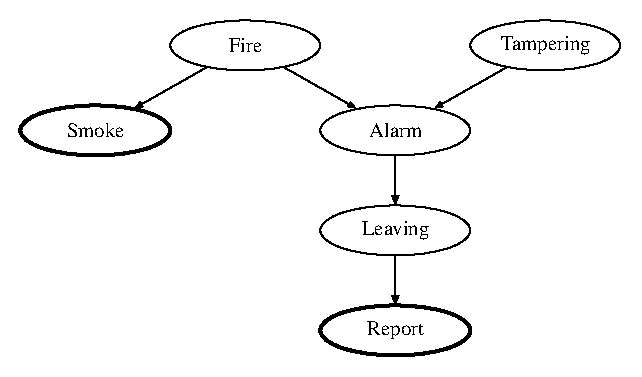
\includegraphics[scale=0.8]{fig/alarm.eps}}
\caption{Example of a discrete Bayesian network.}
\label{fig:alarm}
\end{figure}

\noindent
It is easy to notice that the marginalization above takes an exponential
time with respect to the number of variable to marginalize.  In the
literature of research on Bayesian networks, efficient algorithms
are known to compute such marginalization, but in this section,
we concentrate on how we represent Bayesian networks in PRISM.
Indeed, for a certain class called singly-connected Bayesian networks,
\conindex{Bayesian network!singly-connected ---} it is
shown in \cite{Sato01b} that we can write a PRISM program that
can simulate the Pearl's propagation algorithm.

Now we start to describe the Bayesian network in Figure~\ref{fig:alarm}.
Also for this case, a generative way of thinking should be useful in
writing the modeling part.
For example, we first get the value of {\it Fire} by flipping a coin
(i.e.\ sampling) according to $P({\it Fire})$.  We then proceed to
flip a coin for {\it Smoke} according to $P({\it Smoke}\mid{\it Fire})$,
and so on.  Here we represent such a coin flipping by {\tt msw($I$,$V$)},
and define the joint distribution (Eq.~\ref{eq:bn:joint}) with
a predicate {\tt world/6}:
\progindex{world/6}
\begin{quote}
\begin{verbatim}
world(Fi,Ta,Al,Sm,Le,Re) :-
   msw(fi,Fi),
   msw(ta,Ta),
   msw(sm(Fi),Sm),
   msw(al(Fi,Ta),Al),
   msw(le(Al),Le),
   msw(re(Le),Re).
\end{verbatim}
\end{quote}
This clause indicates that we flip the coins in the order of
{\it Fire}, {\it Tampering}, {\it Smoke}, {\it Alarm}, {\it Leaving}
and {\it Report}.  As is declared later, the switches above are assumed
here to output {\tt yes} or {\tt no}.  The switch named {\tt fi}
corresponds to the coin flipping for {\it Fire}, and switch
{\tt sm(Fi)} corresponds to the coin flipping for {\it Smoke},
given the value of {\it Fire} as {\tt Fi}.  Recall here that
each parameter of these switches corresponds to one entry of
the CPTs\conindex{conditional probability table}
in the target Bayesian network.  For instance,
the parameter $\theta_{\mbox{\footnotesize {\tt sm(yes)},{\tt no}}}$,
the probability of a switch instance {\tt msw(sm(yes),no)} being true,
corresponds to the conditional probability
$P({\it Smoke}={\it no}\mid {\it Fire}={\it yes})$.

The observable distribution is defined by {\tt world/2}:
\progindex{world/2}
\begin{quote}
\begin{verbatim}
world(Sm,Re) :- world(_,_,_,Sm,_,Re).
\end{verbatim}
\end{quote}
The probability of {\tt world(yes,no)} corresponds to
$P({\it Smoke}={\it yes}, {\it Report}={\it no})$.
We can find that, for {\tt world(yes,no)}, all instantiations
of the body are probabilistically exclusive to each other,
so we can compute the probability of {\tt world(yes,no)}
by summing up the probabilities of these instantiations.
This fact corresponds to Eq.~\ref{eq:bn:marginal}, so
we can say the program precisely express what we would like to model.
The model part of our Bayesian network program consists of the
two clauses above.

We add a multi-valued switch declaration which specifies all switches
have outcomes {\tt yes} and {\tt no} as follows:
\begin{quote}
\begin{verbatim}
values(_,[yes,no]).
\end{verbatim}
\end{quote}
\predindex{values/2}

Now let us make a similar experiment to one with the HMM program
(\secref{sec:example:hmm}).  Namely, we first generate goals by
sampling as training data under some predefined parameters, and then
learn the parameters\conindex{parameter learning}
from such training data.  The difference is
that we attempt to {\em fix} (or preserve) one parameter in learning.
Such a parameter can be considered as a constant parameter in
the model.  The utility part\conindex{utility part} may contain the
following batch predicate for the experiment:
\predindex{unfix\_sw/1}\predindex{fix\_sw/1}
\predindex{get\_samples/3}
\predindex{learn/1}
\begin{quote}
\begin{verbatim}
alarm_learn(N) :-
  unfix_sw(_),                  % Make all parameters changeable
  set_params,                   % Set parameters as you specified
  get_samples(N,world(_,_),Gs), % Get N samples
  fix_sw(fi),                   % Preserve the parameter values
  learn(Gs).                    %   for {msw(fi,yes), msw(fi,no)}
\end{verbatim}
\end{quote}
The experimental steps are written as comments.  In this predicate,
{\tt set\_params/0} (which specifies the parameters of all switches;
\secref{sec:built-in:switch:set_sw}),
{\tt get\_samples/3} (which generate training data;
\secref{sec:built-in:sample}), and {\tt learn/1}
(\secref{sec:built-in:learn:em-preds}) are used similarly
to those in the batch routine for the experiments with HMMs
(\secref{sec:example:hmm}).
{\tt set\_params/0} is a user-defined predicate:
\predindex{set\_sw/2}
\begin{quote}
\begin{small}
\begin{verbatim}
set_params :-
  set_sw(fi,[0.1,0.9]),
  set_sw(ta,[0.15,0.85]),
  set_sw(sm(yes),[0.95,0.05]),
  set_sw(sm(no),[0.05,0.95]),
  set_sw(al(yes,yes),[0.50,0.50]),
  set_sw(al(yes,no),[0.90,0.10]),
  set_sw(al(no,yes),[0.85,0.15]),
  set_sw(al(no,no),[0.05,0.95]),
  set_sw(le(yes),[0.88,0.12]),
  set_sw(le(no),[0.01,0.99]),
  set_sw(re(yes),[0.75,0.25]),
  set_sw(re(no),[0.10,0.90]).
\end{verbatim}
\end{small}
\end{quote}

\noindent
As described above, the additional functionality is that we do not learn
(i.e.\ fix or preserve) the parameters for switch {\tt fi}.  This is
done by using the built-ins {\tt unfix\_sw/1} and {\tt fix\_sw/1}
(\secref{sec:built-in:switch:fix_sw}).

Now our PRISM program has been completed, and we are ready to run the program.
Let us assume that the program is contained in the file `{\tt alarm.psm}', then
load the program by the command {\tt prism(alarm)}:\predindex{prism/1}
\predindex{prism/1}
\begin{quote}
\begin{verbatim}
?- prism(alarm).
\end{verbatim}
\end{quote}
We conduct learning with 500 samples by {\tt alarm\_learn/1}
which is previously defined:
\progindex{alarm\_learn/1}
\begin{quote}
\begin{small}
\begin{verbatim}
?- alarm_learn(500).

#goals: 0(4)
Exporting switch information to the EM routine ...
#em-iters: 0(2) (Converged: -464.034430688)
Statistics on learning:
        Graph size: 448
        Number of switches: 12
        Number of switch instances: 24
        Number of iterations: 2
        Final log likelihood: -464.034430688
        Total learning time: 0.004 seconds
        Explanation search time: 0.000 seconds
        Total table space used: 47008 bytes
Type show_sw or show_sw_b to show the probability distributions.
\end{verbatim}
\end{small}
\end{quote}
We can confirm the learned parameters as follows:\predindex{show\_sw/0}
\predindex{show\_sw/0}
\begin{quote}
\begin{small}
\begin{verbatim}
?- show_sw.

Switch fi: fixed_p: yes (p: 0.100000000) no (p: 0.900000000)
Switch ta: unfixed_p: yes (p: 0.682231979) no (p: 0.317768021)
Switch le(no): unfixed_p: yes (p: 0.419688112) no (p: 0.580311888)
Switch le(yes): unfixed_p: yes (p: 0.476437741) no (p: 0.523562259)
Switch re(no): unfixed_p: yes (p: 0.283975504) no (p: 0.716024496)
Switch re(yes): unfixed_p: yes (p: 0.167325271) no (p: 0.832674729)
Switch sm(no): unfixed_p: yes (p: 0.130802678) no (p: 0.869197322)
Switch sm(yes): unfixed_p: yes (p: 0.122775877) no (p: 0.877224123)
Switch al(no,no): unfixed_p: yes (p: 0.480950708) no (p: 0.519049292)
Switch al(no,yes): unfixed_p: yes (p: 0.451939009) no (p: 0.548060991)
Switch al(yes,no): unfixed_p: yes (p: 0.472514062) no (p: 0.527485938)
Switch al(yes,yes): unfixed_p: yes (p: 0.380557386) no (p: 0.619442614)
\end{verbatim}
\end{small}
\end{quote}
It is also possible to get the frequencies of the sampled goals:
\predindex{show\_goals/0}
\begin{quote}
\begin{small}
\begin{verbatim}
?- show_goals.

Goal world(yes,yes) (count=34, freq=6.800%)
Goal world(no,no) (count=353, freq=70.600%)
Goal world(yes,no) (count=31, freq=6.200%)
Goal world(no,yes) (count=82, freq=16.400%)
Total_count=500
\end{verbatim}
\end{small}
\end{quote}

\subsection{Computing conditional probabilities}
\label{sec:example:bn:cprob}

Furthermore, for the Bayesian network program described in this section,
conditional probabilities can be computed as conditional hindsight
probabilities\conindex{hindsight probability!conditional ---}
(\secref{sec:built-in:hindsight}).  Let us recall that
a conditional hindsight probability is denoted as $P_\theta(G'|G)=
P_\theta(G')/P_\theta(G)$, where $G$ is a given top goal and $G'$ is
one of its subgoals.  For instance, let us consider to compute the
conditional probability
$P({\it Alarm}\mid {\it Smoke}={\it yes}, {\it Report}={\it no})$
by using conditional hindsight probabilities.
Since the target conditional probability
$P({\it Alarm}=x\mid {\it Smoke}={\it yes}, {\it Report}={\it no})$
can be computed as
$P({\it Alarm}=x, {\it Smoke}={\it yes}, {\it Report}={\it no})/
P({\it Smoke}={\it yes}, {\it Report}={\it no})$, if we let
$G$ = {\tt world(\_,\_,\_,yes,\_,no)}
and $G'$ = {\tt world(\_,\_,$x$,yes,\_,no)},
it can be seen that $P_\theta(G'|G)$ is equal to the target
conditional probability.
To get the conditional distribution on {\it Alarm}, we run
{\tt chindsight\_agg/2}\predindex{chindsight\_agg/2}
with specifying the third argument in {\tt world/6}
(which corresponds to {\it Alarm}) as a query argument:\footnote{
In this computation, it is assumed that the parameters are set by
{\tt set\_params/0} in advance.
}

\predindex{chindsight\_agg/2}
\progindex{world/6}
\begin{quote}
\begin{small}
\begin{verbatim}
?- chindsight_agg(world(_,_,_,yes,_,no),world(_,_,query,yes,_,no)).
conditional hindsight probabilities:
  world(*,*,no,yes,*,no): 0.620773027495463
  world(*,*,yes,yes,*,no): 0.379226972504537
\end{verbatim}
\end{small}
\end{quote}

\noindent
Of course, from the definition of {\tt world/2}, we can make
the same computation with {\tt world/2}:

\predindex{chindsight\_agg/2}
\progindex{world/2}
\progindex{world/6}
\begin{quote}
\begin{small}
\begin{verbatim}
?- chindsight_agg(world(yes,no),world(_,_,query,yes,_,no)).
conditional hindsight probabilities:
  world(*,*,no,yes,*,no): 0.620773027495463
  world(*,*,yes,yes,*,no): 0.379226972504537
\end{verbatim}
\end{small}
\end{quote}

\noindent
As mentioned before, the definition of {\tt world/6} is computationally naive,
so we need to write a different representation of Bayesian networks which takes
into account the computational effort for conditional hindsight probabilities,
as shown in the next section.

\exindex{alarm network program|)}

\subsection{Bayesian networks in junction-tree form}
\label{sec:example:bn:jt}

For probabilistic inferences on Bayesian networks, especially, on multiply-connected
Bayesian networks (BNs),\conindex{Bayesian network!multiply-connected ---}
several sophisticated techniques have been proposed so far. As another example of a BN,
let us consider a Bayesian network called the Asia network~\cite{Lauritzen88},
which is illustrated in Figure~\ref{fig:asia}.  This network can be said to be
a multiply-connected BN since there are two paths from $S$ to $D$:
$S\to L\to\mathit{TL}\to D$ and $S\to B\to D$.  One of the most
popular inference methods for such multiply-connected BNs is the junction-tree
algorithm.\conindex{junction tree!--- algorithm}
In the junction-tree algorithm, we first convert the original network
to an undirected tree-structured network called a junction tree,\conindex{junction tree}
whose node corresponds to a set consisting of one or more original nodes.
Figure~\ref{fig:jasia} depicts a junction tree for the Asia network.
For example, $\alpha_2$ in Figure~\ref{fig:jasia} corresponds to
a set $\{S,L,B\}$ of the original nodes
in Figure~\ref{fig:asia}.

\begin{figure}[tbp]
\centerline{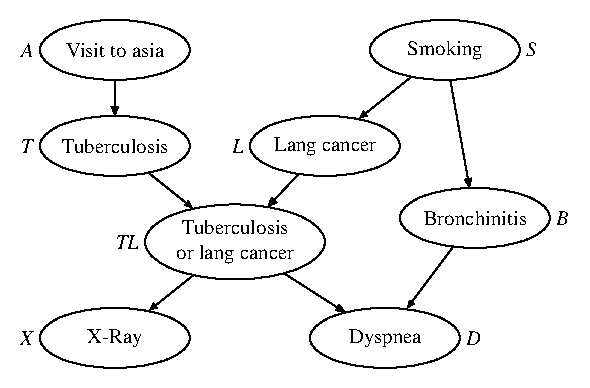
\includegraphics[scale=0.85]{fig/asia.eps}}
\caption{Example of a multiply-connected Bayesian network\conindex{Bayesian network!multiply-connected ---} (known as the Asia network).}
\label{fig:asia}
\end{figure}

\exindex{Asia network program!naive version of ---|(}

We can write a `naive' version of the PRISM program that represents the Asia
network as did in the previous section.  Also in this program, all switches are
supposed to be binary, i.e.\ they take values `{\tt t}' (true) and `{\tt f}' (false).
{\tt incl\_or/3}\progindex{incl\_or/3} represents the inclusive OR.
We set the parameters given in \cite{Lauritzen88} by {\tt set\_params/0}.

\progindex{world/4}
\progindex{world/6}
\progindex{incl\_or/3}
\progindex{set\_params/0}
\begin{quote}
\begin{small}
\begin{verbatim}
values(bn(_,_),[t,f]).

world(A,S,X,D):- world(A,_,S,_,_,X,_,D).

world(A,T,S,L,TL,X,B,D) :-
   msw(bn(a,[]),A),msw(bn(t,[A]),T),
   msw(bn(s,[]),S),msw(bn(l,[S]),L),
   incl_or(T,L,TL),
   msw(bn(x,[TL]),X),msw(bn(b,[S]),B),
   msw(bn(d,[TL,B]),D).

incl_or(t,t,t).
incl_or(t,f,t).
incl_or(f,t,t).
incl_or(f,f,f).

:- set_params.

set_params:-
  set_sw(bn(a,[]),[0.01,0.99]),
  set_sw(bn(t,[t]),[0.05,0.95]),
  set_sw(bn(t,[f]),[0.01,0.99]),
  set_sw(bn(s,[]),[0.5,0.5]),
  set_sw(bn(l,[t]),[0.1,0.9]),
  set_sw(bn(l,[f]),[0.01,0.99]),
  set_sw(bn(x,[t]),[0.98,0.02]),
  set_sw(bn(x,[f]),[0.05,0.95]),
  set_sw(bn(b,[t]),[0.60,0.40]),
  set_sw(bn(b,[f]),[0.30,0.70]),
  set_sw(bn(d,[t,t]),[0.90,0.10]),
  set_sw(bn(d,[t,f]),[0.70,0.30]),
  set_sw(bn(d,[f,t]),[0.80,0.20]),
  set_sw(bn(d,[f,f]),[0.10,0.90]).
\end{verbatim}
\end{small}
\end{quote}

\begin{figure}[tbp]
\centerline{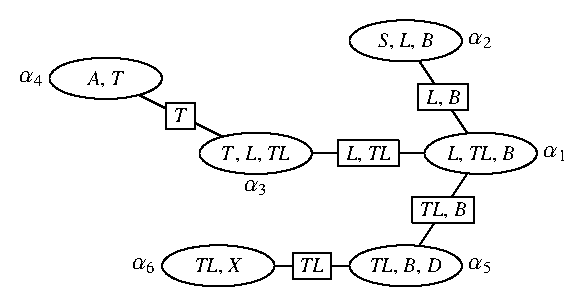
\includegraphics[scale=1.0]{fig/jasia.eps}}
\caption{Junction tree\conindex{junction tree} for the Asia network.}
\label{fig:jasia}
\end{figure}

\noindent
After loading the program, for example, we can compute the conditional distribution
$P(T=\mathit{true}\mid A=\mathit{false}, D=\mathit{true})=0.018$ and
$P(T=\mathit{false}\mid A=\mathit{false}, D=\mathit{true})=0.982$ as follows:
\predindex{chindsight\_agg/2}
\begin{quote}
\begin{small}
\begin{verbatim}
?- chindsight_agg(world(f,_,_,t),world(_,query,_,_,_,_,_,_)).
conditional hindsight probabilities:
  world(*,f,*,*,*,*,*,*): 0.981873562361255
  world(*,t,*,*,*,*,*,*): 0.018126437638745
\end{verbatim}
\end{small}
\end{quote}
\exindex{Asia network program!naive version of ---|)}
Surely this program returns the consistent results, but is not so efficient.
On the other hand, let us see another PRISM program that represents a junction
tree and is expected to run faster than the naive version.
For the readers who are interested in the formal discussion on such
PRISM programs in junction-tree form, please consult \cite{Sato07,Sato08}.
\exindex{Asia network program!junction-tree version of ---|(}
For instance, the following is a junction-tree version of the PRISM program
for the Asia network:
\progindex{world/1}
\progindex{cpt/4}
\exindex{node predicates@{\tt node\_$i$} predicates}
\exindex{msg predicates@{\tt msg\_$i$\_$j$} predicates}
\begin{quote}
\begin{small}
\begin{verbatim}
values(bn(_,_),[t,f]).

world(E):- msg_1_0(E-[]).

msg_1_0(E0-E1)      :- node_1(L,TL,B,E0-E1).
msg_2_1(L,B,E0-E1)  :- node_2(S,L,B,E0-E1).
msg_3_1(L,TL,E0-E1) :- node_3(T,L,TL,E0-E1).
msg_4_3(T,E0-E1)    :- node_4(A,T,E0-E1).
msg_5_1(TL,B,E0-E1) :- node_5(TL,B,D,E0-E1).
msg_6_5(TL,E0-E1)   :- node_6(TL,X,E0-E1).

node_1(L,TL,B,E0-E1) :-
    msg_2_1(L,B,E0-E2),msg_3_1(L,TL,E2-E3),msg_5_1(TL,B,E3-E1).
node_2(S,L,B,E0-E1)  :-
    cpt(s,[],S,E0-E2),cpt(l,[S],L,E2-E3),cpt(b,[S],B,E3-E1).
node_3(T,L,TL,E0-E1) :- incl_or(L,T,TL),msg_4_3(T,E0-E1).
node_4(A,T,E0-E1)    :- cpt(a,[],A,E0-E2),cpt(t,[A],T,E2-E1).
node_5(TL,B,D,E0-E1) :- cpt(d,[TL,B],D,E0-E2),msg_6_5(TL,E2-E1).
node_6(TL,X,E0-E1)   :- cpt(x,[TL],X,E0-E1).

cpt(X,Par,V,E0-E1):- ( E0=[(X,V)|E1] -> true ; E0=E1 ),msw(bn(X,Par),V).

incl_or(t,t,t).
incl_or(t,f,t).
incl_or(f,t,t).
incl_or(f,f,f).
\end{verbatim}
\end{small}
\end{quote}
In this program, we consider that $\alpha_1$ in Figure~\ref{fig:jasia}
is the root node of the junction tree.  The predicate whose name is
{\tt msg\_$i$\_$j$}\exindex{msg predicates@{\tt msg\_$i$\_$j$} predicates}
corresponds to the edge between nodes $i$ and $j$ in the junction tree.
We also define a predicate named
{\tt node\_$i$}\exindex{node predicates@{\tt node\_$i$} predicates}
for each node $i$ in the junction tree.  One may find that the evidences\conindex{evidence}
will be kept as difference lists\conindex{difference list} in the last arguments of the
{\tt msg\_$i$\_$j$} and the {\tt node\_$i$} predicates.  We can
input evidences through the argument of {\tt world/1}, but for simplicity,
the evidences are assumed here to be given in the same order as that of
the appearances of {\tt msw/2} in the top-down execution of
{\tt world/1}.  {\tt cpt/4}\progindex{cpt/4} is a wrapper predicate that
can handle evidences.  We omit here {\tt set\_params/0} which is also included
in the naive version.

Using this program, let us compute the conditional distribution
$P(T\mid A=\mathit{false}, D=\mathit{true})$.  To realize this,
We attempt to compute the hindsight probabilities for the predicate
{\tt node\_4/3} since $\alpha_4$ includes the original node
(i.e. the random variable) $T$, as shown in Figure~\ref{fig:jasia}.
\predindex{chindsight\_agg/2}
\exindex{node predicates@{\tt node\_$i$} predicates}
\begin{quote}
\begin{small}
\begin{verbatim}
?- chindsight_agg(world([(a,f),(d,t)]),node_4(_,query,_)).
conditional hindsight probabilities:
  node_4(*,f,*): 0.981873562361255
  node_4(*,t,*): 0.018126437638745
\end{verbatim}
\end{small}
\end{quote}
It is proved in \cite{Sato07} that this hindsight computation is equivalent
to the belief propagation procedure\conindex{belief propagation} in a
junction tree.

Instead of using difference lists, we can take evidences into account by adding
them into the Prolog database before making probabilistic inferences.  That is,
we may write:
\progindex{world/1}
\progindex{cpt/3}
\progindex{assert\_evid/1}
\exindex{node predicates@{\tt node\_$i$} predicates}
\exindex{msg predicates@{\tt msg\_$i$\_$j$} predicates}
\begin{quote}
\begin{small}
\begin{verbatim}
world(Es):- assert_evid(Es),msg_1_0.

msg_1_0      :- node_1(_L,_TL,_B).
msg_2_1(L,B) :- node_2(_S,L,B).
msg_3_1(L,TL):- node_3(_T,L,TL).
msg_4_3(T)   :- node_4(_A,T).
msg_5_1(TL,B):- node_5(TL,B,_D).
msg_6_5(TL)  :- node_6(TL,_X).

node_1(L,TL,B):- msg_2_1(L,B),msg_3_1(L,TL),msg_5_1(TL,B).
node_2(S,L,B) :- cpt(s,[],S),cpt(l,[S],L),cpt(b,[S],B).
node_3(T,L,TL):- incl_or(L,T,TL),msg_4_3(T).
node_4(A,T)   :- cpt(a,[],A),cpt(t,[A],T).
node_5(TL,B,D):- cpt(d,[TL,B],D),msg_6_5(TL).
node_6(TL,X)  :- cpt(x,[TL],X).

cpt(X,Par,V):- ( evid(X,V) -> true ; true ),msw(bn(X,Par),V).

incl_or(t,t,t).
incl_or(t,f,t).
incl_or(f,t,t).
incl_or(f,f,f).

assert_evid(Es):- retractall(evid(_,_)),assert_evid0(Es).
assert_evid0([]).
assert_evid0([(X,V)|Es]):- assert(evid(X,V)),!,assert_evid0(Es).
\end{verbatim}
\end{small}
\end{quote}
It is obvious that this program is simpler and more flexible than the one with
difference lists.  On the other hand, we should note that the program's
declarative semantics has been lost, and that in learning, the subgoals are
inappropriately shared among the observed goals, each of which is associated
with a different set of evidences.\footnote{
This optimization is called inter-goal sharing,\conindex{inter-goal sharing}
and unconditionally enabled in the current programming system.  An ad-hoc
workaround is to introduce an ID for each set of evidences and keep the ID
through the arguments (e.g.\ we define {\tt world(ID,E)}, {\tt msg\_2\_1(ID,L,B)},
and so on).
}
\exindex{Asia network program!junction-tree version of ---|)}

It is possible to implement a translator (including a junction-tree constructor)
from a network specification in some standard format (e.g.\ XMLBIF) to a PRISM program
of the corresponding junction tree.  Since version 1.12.1, a Java implementation
of such a translator, named {\tt BN2Prism},\progindex{BN2Prism} is included
under the {\tt exs/jtree} directory in the released package.
{\tt BN2Prism} uses a tree-decomposition technique described in \cite{Kask05}
to generate a PRISM program in junction-tree form\footnote{
To be exact, a PRISM program generated by {\tt BN2Prism} has a graph structure
called a {\em bucket tree}.\conindex{bucket tree}  For details, please see
the documents under the {\tt exs/jtree/bn2prism/doc} directory.
The {\em bucket-tree elimination}\conindex{bucket tree!--- elimination} algorithm
is a message-passing algorithm on a bucket tree~\cite{Kask05}.
}
and such a decomposition technique can be a bridge from PRISM to probabilistic-logical
modeling/inference systems based on Bayesian networks.

\begin{table}
\caption{CPT for {\it Alarm} constructed by the noisy-OR rule}
\label{tab:alarm}
\centerline{
\begin{tabular}{|cc|l|l|}
\hline
{\it Fire}&{\it Tampering}&\multicolumn{1}{|c|}{$P(\mathit{alarm})$}&\multicolumn{1}{|c|}{$P(\neg\mathit{alarm})$}\\
\hline
{\it true}&{\it true}&$0.94=1-0.3\times 0.2$&$0.06=0.3\times 0.2$\\
{\it true}&{\it false}&$0.7=1-0.3$&0.3\\
{\it false}&{\it true}&$0.8=1-0.2$&0.2\\
{\it false}&{\it false}&0&1\\
\hline
\end{tabular}
}
\end{table}

\subsection{Using noisy OR}
\label{sec:example:bn:noisy-or}

In modeling with Bayesian networks, we sometimes use {\em combination rules}
\conindex{combination rule} to make the CPTs simpler, and
{\em noisy OR}\conindex{noisy OR} is one of the most well-known combination
rules~\cite{Russell02}.  To be specific, let us consider the alarm network
(Figure~\ref{fig:alarm}) again, and suppose that the {\it Alarm} node in
the alarm network has a CPT defined with the noisy-OR rule.  Also we suppose
that the individual inhibition probabilities\conindex{noisy OR!inhibition probability in ---}
are given as follows:\footnote{
We denote the propositions $\mathit{Alarm}=\mathit{true}$,
$\mathit{Alarm}=\mathit{false}$, $\mathit{Fire}=\mathit{true}$,
and so on by $\mathit{alarm}$, $\neg\mathit{alarm}$,
$\mathit{fire}$, and so on, respectively.
}
\begin{eqnarray*}
P(\neg\mathit{alarm}\mid\mathit{fire},\neg\mathit{tampering})&=&0.3\\
P(\neg\mathit{alarm}\mid\neg\mathit{fire},\mathit{tam-paring})&=&0.2.
\end{eqnarray*}
Then we have a CPT for {\it Alarm} shown in Table~\ref{tab:alarm}.
To write the alarm network program that deals with the noisy-OR rules,
we modify the definitions of {\tt world/6} and introduce the predicates named
{\tt cpt\_$x$} for each variable named $x$.  Then {\tt world/6} calls such 
{\tt cpt\_$x$} predicates instead of directly calling random switches.
The modeling part of the resulting program is as follows:

\exindex{alarm network program!--- using noisy OR}
\progindex{world/6}
\progindex{cpt\_al/3}
\begin{quote}
\begin{small}
\begin{verbatim}
world(Fi,Ta,Al,Sm,Le,Re) :-
   cpt_fi(Fi),
   cpt_ta(Ta),
   cpt_sm(Fi,Sm),
   cpt_al(Fi,Ta,Al),
   cpt_le(Al,Le),
   cpt_re(Le,Re).

cpt_fi(Fi):- msw(fi,Fi).
cpt_ta(Ta):- msw(ta,Ta).
cpt_sm(Fi,Sm):- msw(sm(Fi),Sm).
cpt_al(Fi,Ta,Al):-
   ( Fi = yes, Ta = yes ->
       msw(cause_al_fi,N_Al_Fi),
       msw(cause_al_ta,N_Al_Ta),
       ( N_Al_Fi = no, N_Al_Ta = no -> Al = no
       ; Al = yes
       )
   ; Fi = yes, Ta = no  -> msw(cause_al_fi,Al)
   ; Fi = no,  Ta = yes -> msw(cause_al_ta,Al)
   ; Fi = no,  Ta = no  -> Al = no
   ).
cpt_le(Al,Le):- msw(le(Al),Le).
cpt_re(Le,Re):- msw(re(Le),Re).
\end{verbatim}
\end{small}
\end{quote}
It can be seen that {\tt cpt\_al/3}\progindex{cpt\_al/3} is an implementation of
the noisy-OR rule.
The key step is to consider the generation process\conindex{generation process} underlying
the noisy-OR rule.
For example, when $\mathit{Fire}=\mathit{true}$ and $\mathit{Tampering}=\mathit{true}$,
we make choices twice by random switches named {\tt cause\_\lb al\_\lb fi}
and {\tt cause\_\lb al\_\lb ta} according to the corresponding
inhibition probabilities.\conindex{noisy OR!inhibition probability in ---}
Then, if one of these choices returns {\tt yes}, we consider that {\it Alarm} becomes true.
 
Let us further write a more generic version.  We first write the
network-specific part of the model by modifying the definition of
{\tt world/6} and by adding {\tt noisy\_or/3} for the specifications of
noisy-OR nodes:
\progindex{world/2}
\progindex{world/6}
\progindex{noisy\_or/3}
\begin{quote}
\begin{small}
\begin{verbatim}
world(Sm,Re):- world(_,_,_,Sm,_,Re).

world(Fi,Ta,Al,Sm,Le,Re) :-
   cpt(fi,[],Fi),
   cpt(ta,[],Ta),
   cpt(sm,[Fi],Sm),
   cpt(al,[Fi,Ta],Al),
   cpt(le,[Al],Le),
   cpt(re,[Le],Re).

noisy_or(al,[fi,ta],[[0.7,0.3],[0.8,0.2]]).
\end{verbatim}
\end{small}
\end{quote}
In the above, {\tt cpt/3} in the clause body of {\tt world/6} is an abstract
(or a wrapper) predicate that can deal with the noisy-OR rule, and its definition
is included in the network-independent part of the model:
\progindex{choose\_noisy\_or/4}
\progindex{choose\_noisy\_or/6}
\begin{quote}
\begin{small}
\begin{verbatim}
:- p_not_table choose_noisy_or/4, choose_noisy_or/6.

cpt(X,PaVs,V):-
   ( noisy_or(X,Pa,_) -> choose_noisy_or(X,Pa,PaVs,V)
   ; msw(bn(X,PaVs),V)
   ).

choose_noisy_or(X,Pa,PaVs,V):- choose_noisy_or(X,Pa,PaVs,no,no,V).

choose_noisy_or(_,[],[],yes,V,V).
choose_noisy_or(_,[],[],no,_,no).
choose_noisy_or(X,[Y|Pa],[PaV|PaVs],PaHasYes0,ValHasYes0,V):-
   ( PaV=yes ->
       msw(cause(X,Y),V0),
       PaHasYes=yes,
       ( ValHasYes0=no, V0=no -> ValHasYes=no
       ; ValHasYes=yes
       )
   ; PaHasYes=PaHasYes0,
     ValHasYes=ValHasYes0
   ),
   choose_noisy_or(X,Pa,PaVs,PaHasYes,ValHasYes,V).
\end{verbatim}
\end{small}
\end{quote}
{\tt choose\_noisy\_or/4} is a generalization of {\tt cpt\_al/3} described above.
Some might feel this network-independent part procedural, but conversely we can say
that this exhibits the flexibility of the PRISM (and underlying Prolog) language.
It is also possible to put the definition of {\tt choose\_noisy\_\lb or/4}
into a separate library file loaded by the inclusion declaration\conindex{inclusion declaration}
(\secref{sec:lang:decl:include}), and then the network-specific part
(namely, the definitions of {\tt world/2}, {\tt world/6} and {\tt noisy\_or/3}) will be
left more declarative.  The PRISM language only provides a simple built-in
probabilistic predicate implementing random switches, but as long as we deal with
generative models, there seems to be ways to construct a more abstract formalism
combining these random switches.  The {\tt p\_not\_table}\declindex{p\_not\_table}
declarations are added for making the inference results simple and readable.

The utility part should be modified accordingly.  First, we add a couple of
batch routines for setting parameters:
\begin{quote}
\begin{small}
\begin{verbatim}
set_params:-
   set_sw(bn(fi,[]),[0.1,0.9]),
   set_sw(bn(ta,[]),[0.15,0.85]),
   set_sw(bn(sm,[yes]),[0.95,0.05]),
   set_sw(bn(sm,[no]),[0.05,0.95]),
   set_sw(bn(le,[yes]),[0.88,0.12]),
   set_sw(bn(le,[no]),[0.01,0.99]),
   set_sw(bn(re,[yes]),[0.75,0.25]),
   set_sw(bn(re,[no]),[0.10,0.90]).

set_nor_params:-
   ( noisy_or(X,Pa,DistList),
     set_nor_params(X,Pa,DistList),
     fail
   ; true
   ).

set_nor_params(_,[],[]).
set_nor_params(X,[Y|Pa],[Dist|DistList]):-
   set_sw(cause(X,Y),Dist),!,
   set_nor_params(X,Pa,DistList).

:- set_params.
:- set_nor_params.
\end{verbatim}
\end{small}
\end{quote}
In the above, {\tt set\_nor\_params/0} sets the switch parameters according
to the specifications of the noisy-OR nodes.  To confirm whether the
network-independent part of the model works well, let us introduce
the following routines:
\predindex{prob/1}
\predindex{probf/1}
\begin{quote}
\begin{small}
\begin{verbatim}
print_dist_al:-
   ( member(Fi,[yes,no]),
     member(Ta,[yes,no]),
     member(Al,[yes,no]),
     get_cpt_prob(al,[Fi,Ta],Al,P),
     format("P(al=~w | fi=~w, ta=~w):~t~6f~n",[Al,Fi,Ta,P]),
     fail
   ; true
   ).

print_expl_al:-
   ( member(Fi,[yes,no]),
     member(Ta,[yes,no]),
     member(Al,[yes,no]),
     get_cpt_probf(al,[Fi,Ta],Al),
     fail
   ; true
   ).

get_cpt_prob(X,PaVs,V,P):-
   ( prob(cpt(X,PaVs,V),P)
   ; P = 0.0
   ),!.

get_cpt_probf(X,PaVs,V):-
   ( probf(cpt(X,PaVs,V))
   ; format("cpt(~w,~w,~w): always false~n",[X,PaVs,V])
   ),!.
\end{verbatim}
\end{small}
\end{quote}
{\tt print\_dist\_al/0} shows the distribution of the {\it Alarm} node
for each instantiations of its parents by a failure-driven loop, and
{\tt print\_expl\_al/0} shows a logical expression of the probabilistic
behavior of the {\it Alarm} node.  {\tt get\_cpt\_prob/4}
and {\tt get\_cpt\_probf/3} are just introduced for dealing with
the cases that {\tt prob/2} or {\tt probf/1} fails.
Finally, we can confirm that the generic version of the alarm network
program with the noisy-OR rule works correctly:
\begin{quote}
\begin{small}
\begin{verbatim}
?- print_dist_al.

P(al=yes | fi=yes, ta=yes):     0.940000
P(al=no | fi=yes, ta=yes):      0.060000
P(al=yes | fi=yes, ta=no):      0.700000
P(al=no | fi=yes, ta=no):       0.300000
P(al=yes | fi=no, ta=yes):      0.800000
P(al=no | fi=no, ta=yes):       0.200000
P(al=yes | fi=no, ta=no):       0.000000
P(al=no | fi=no, ta=no):        1.000000

?- print_expl_al.

cpt(al,[yes,yes],yes)
   <=> msw(cause(al,fi),yes) & msw(cause(al,ta),yes)
     v msw(cause(al,fi),yes) & msw(cause(al,ta),no)
     v msw(cause(al,fi),no) & msw(cause(al,ta),yes)
cpt(al,[yes,yes],no)
   <=> msw(cause(al,fi),no) & msw(cause(al,ta),no)
cpt(al,[yes,no],yes)
   <=> msw(cause(al,fi),yes)
cpt(al,[yes,no],no)
   <=> msw(cause(al,fi),no)
cpt(al,[no,yes],yes)
   <=> msw(cause(al,ta),yes)
cpt(al,[no,yes],no)
   <=> msw(cause(al,ta),no)
cpt(al,[no,no],yes): always false
cpt(al,[no,no],no)
\end{verbatim}
\end{small}
\end{quote}

Here, one may think from the iff-formula for {\tt cpt(al,[yes,yes],yes)}
that the number of sub-explanations for {\tt cpt(al,$\cdot$,yes)} can
exponentially grows as the {\it Alarm} node has more parent nodes.
This problem comes from the modeling assumption (i.e.\ the exclusiveness condition)
\conindex{exclusiveness condition} that the sub-explanations should
be exclusive to each other.
On the other hand, if we could use inclusive OR, the iff-formula will
be much simplified as follows:
\[
\mbox{\tt cpt(al,[yes,yes],yes)}
\Leftrightarrow
\mbox{\tt msw(cause(al,fi),yes)}\lor\mbox{\tt msw(cause(al,ta),yes)}.
\]
Recent works~\cite{DeRaedt07,Ishihata08,Ishihata10} introduce
binary decision diagrams\conindex{binary decision diagram} (BDDs)
\conindex{BDD|see{binary decision diagram}} for probability inferences
based on logical expressions, where inclusive disjunctions are
automatically converted into exclusive disjunctions in a compressed form.
The programming system should incorporate such mechanisms in future.

\exindex{Bayesian network program|)}


%% \section{Model selection}
%% \label{sec:example:msel}


\section{Statistical analysis}
\label{sec:example:analysis}

PRISM is a suitable tool for analyzing statistical data.  In this section, we
present three examples.  In the first example, we consider gene inheritance
of human's blood type again, and show a typical way to answer the question
of model selection.  The second example attempts to find a probabilistic
justification for a common practice seen in tennis games: players serve
second services more conservatively than first services. We write a program
to demonstrate that the percentage of points won would normally decline
should a player serve second services as hard as first ones. The third example
attempts to obtain statistics that can be used to tune the unification procedure.


\subsection{Another hypothesis on blood type inheritance}
\label{sec:example:analysis:blood}
\exindex{blood type program!AaBb ---|(}

The ABO gene model on the inheritance of ABO blood type,\exindex{ABO gene model}
described in \secref{sec:overview:basic}, was introduced in early 20th century~\cite{Crow83}.
Around that time, there was another hypothesis that we have two loci for ABO blood type
with dominant alleles A/a and B/b.  According to this hypothesis, genotypes aabb,
A$\ast$bb, aaB$\ast$ and A$\ast$B$\ast$ correspond to the blood types
(phenotypes) O, A, B and AB, respectively, where $\ast$ stands for a ``don't care'' symbol.
In this section, let us call this hypothesis the AaBb gene model.\exindex{AaBb gene model}
The following is a PRISM program for the AaBb gene model:

\progindex{bloodtype/1}
\progindex{genotype/3}
\begin{quote}
\begin{verbatim}
%%%%  Declarations:

:- set_prism_flag(data_source,file('bloodtype.dat')).

values(locus1,['A',a]).
values(locus2,['B',b]).

%%%%  Modeling part:

bloodtype(P) :-
   genotype(locus1,X1,Y1),
   genotype(locus2,X2,Y2),
   ( X1=a, Y1=a, X2=b, Y2=b -> P=o 
   ; ( X1='A' ; Y1='A' ), X2=b, Y2=b -> P=a
   ; X1=a, Y1=a, ( X2='B' ; Y2='B')  -> P=b
   ; P=ab
   ).

genotype(L,X,Y) :- msw(L,X),msw(L,Y).
\end{verbatim}
\end{quote}

\noindent
In this program, we use two random switches each of which represents a random
pick-up of a gene in the corresponding locus.  The question here is which hypothesis
from these two hypotheses on blood type inheritance (i.e.\ the ABO gene model and
the AaBb gene model) is more plausible.  To answer this question, we consider
to use a Bayesian model score called BIC (Bayesian Information Criterion).
\conindex{Bayesian Information Criterion}  One may notice that this is
an example of a model selection\conindex{model selection} problem.

Suppose that {\tt bloodABO.psm} and {\tt bloodAaBb.psm} are the program files
for the ABO gene model (given in \secref{sec:overview:basic}) and for
the AaBb gene model (given just above), respectively.  We also assume
that a data file named {\tt bloodtype.dat} which contains 38 persons of
blood type A, 22 persons of blood type B, 31 persons of blood type O and
9 persons of blood type AB.  The ratio of frequencies of blood types in
this data is almost the same as that in Japanese people.  Lastly,
for simplicity, we consider that both programs have the following flag specification:

\begin{quote}
\begin{verbatim}
:- set_prism_flag(data_source,file('bloodtype.dat')).
\end{verbatim}
\end{quote}

Under these settings, we first load {\tt bloodABO.psm}, and then call a
built-in for EM learning.  Finally we can get the BIC value as
$-132.667082$:

\predindex{learn/0}
\predindex{learn\_statistics/2}
\begin{quote}
\begin{small}
\begin{verbatim}
?- prism(bloodABO).
  :
?- learn.
#goals: 0(4)
Exporting switch information to the EM routine ...
#em-iters: 0(5) (Converged: -128.061911600)
Statistics on learning:
        Graph size: 27
        Number of switches: 1
        Number of switch instances: 3
        Number of iterations: 5
        Final log likelihood: -128.061911600
        Total learning time: 0.004 seconds
        Explanation search time: 0.000 seconds
        Total table space used: 5888 bytes
Type show_sw or show_sw_b to show the probability distributions.

yes
?- show_sw.
Switch gene: unfixed_p: a (p: 0.272288804) b (p: 0.169511387) o (p: 0.55
8199809)
  :
?- learn_statistics(bic,BIC).
BIC = -132.667081786147037 ?
\end{verbatim}
\end{small}
\end{quote}

\noindent
On the other hand, we repeat the same procedure for {\tt bloodAaBb.psm},
and get the BIC value as $-135.649847$:

\predindex{learn/0}
\predindex{learn\_statistics/2}
\begin{quote}
\begin{small}
\begin{verbatim}
?- prism(bloodAaBb).
  :
?- learn.
#goals: 0(4)
Exporting switch information to the EM routine ...
#em-iters: 0(5) (Converged: -131.044676485)
Statistics on learning:
        Graph size: 48
        Number of switches: 2
        Number of switch instances: 4
        Number of iterations: 5
        Final log likelihood: -131.044676485
        Total learning time: 0.004 seconds
        Explanation search time: 0.000 seconds
        Total table space used: 7808 bytes
Type show_sw or show_sw_b to show the probability distributions.

yes
?- show_sw.
Switch locus1: unfixed_p: A (p: 0.272006612) a (p: 0.727993388)
Switch locus2: unfixed_p: B (p: 0.169341684) b (p: 0.830658316)
  :
?- learn_statistics(bic,BIC).
BIC = -135.649846671234258 ?
\end{verbatim}
\end{small}
\end{quote}

\noindent
As a result, the ABO gene model has a larger BIC value, so we
can conclude that the ABO gene model is more plausible than the AaBb
gene model according to the data in {\tt bloodtype.dat}.

\exindex{blood type program!AaBb ---|)}


\subsection{Why not serving second services as hard in tennis?}
\label{sec:example:analysis:tennis}
\exindex{tennis program|(}

In tennis games, we observe a common practice, namely, players normally serve second services much more conservatively than serving first services. Most people accept the practice without asking why. We write a program to model the statistical relationship between serving and winning in tennis games and use real statistics of Andy Roddick, one of top players, to answer the question.

In tennis, a player has at most two chances to serve in each point. If the first service is a fault, he has another chance to serve. If both services are faults, he loses the point. The following program models this process.

\predindex{values/2}
\begin{quote}
\begin{verbatim}
values(serve(_),[in,out]).    % switches serve(1) serve(2)
values(result(_),[win,loss]). % switches result(1) result(2)

play(Res):-    % the predicate to be observed
   msw(serve(1),S1),
   ( S1 == in -> msw(result(1),Res)
   ; msw(serve(2),S2),
     ( S2 == in -> msw(result(2),Res)
     ; Res = loss
     )
   ).
\end{verbatim}
\end{quote}

We use two switches, {\tt serve(1)} and {\tt serve(2)}, to represent the outcomes
of services, and use another two switches, {\tt result(1)} and {\tt result(2)},
to represent the results: {\tt result(1)} gives the result of the point when
the first service is legal and {\tt result(2)} the result of the point when
the second service is legal. The result is loss if both services are faults.


The following sets the parameters of the switches based on
Andy Roddick's statistics: his serving percentages are 61 and 95
at first and second services, respectively, and his percentages
of points won at two services are 81 and 56, respectively.

\predindex{set\_sw/2}
\begin{quote}
\begin{verbatim}
roddick:-
   set_sw(serve(1),[0.61,0.39]),
   set_sw(serve(2),[0.95,0.05]),
   set_sw(result(1),[0.81,0.19]),
   set_sw(result(2),[0.56,0.44]).
\end{verbatim}
\end{quote}

\noindent
From the program and the switch parameters, we know Andy Roddick's wining probability is 0.70158.

\predindex{prob/2}
\begin{quote}
\begin{verbatim}
?- prob(play(win),Prob)
Prob = 0.70158
\end{verbatim}
\end{quote}

\noindent
If Andy Roddick served second services like first services, the predicate {\tt play} should be redefined as follows:

\begin{quote}
\begin{verbatim}
play(Res):-
   msw(serve(1),S1),
   ( S1 == in -> msw(result(1),Res)
   ; msw(serve(1),S2),
     ( S2 == in -> msw(result(1),Res)
     ; Res = loss
     )
   ).
\end{verbatim}
\end{quote}

\noindent
His winning probability would decline to 0.686799. This explains why serious tennis players serve second services much more conservatively than first services although the percentage of points won at first services is much higher than that at second services.

\exindex{tennis program|)}

\subsection{Tuning the unification procedure}
\label{sec:example:analysis:tune}
\exindex{unification program|(}

Given two terms, the unification procedure determines if they are unifiable, and if so finds a substitution for the variables in the two terms to make them identical. A term is one of the following four types: {\it variable}, {\it atomic}, {\it list}, and {\it structure}. The unification procedure behaves as follows:

\begin{tabbing}
aaa \= aaa \= aaa \= aaa \= aaa \= aaa \= aaa \kill
\>   unify($t_1$,$t_2$) \{ \\
\>\>   if ($t_1$ is variable) bind $t_1$ to $t_2$;\\
\>\>   else if ($t_1$ is atomic) \{ \\
\>\>\>      if ($t_2$ is variable) bind $t_2$ to $t_1$;\\
\>\>\>      else return $t_1$==$t_2$;\\
\>\>   \} else if ($t_1$ is a list) \{\\
\>\>\>      if ($t_2$ is variable) bind $t_2$ to $t_1$;\\
\>\>\>       else if ($t_2$ is a list) \\
\>\>\> \>         return unify(car($t_1$),car($t_2$)) \&\& unify(cdr($t_1$),cdr($t_2$));\\
\>\>\>       else return false;\\
\>\>    \} else if ($t_1$ is a structure) \{\\
\>\>\>       if ($t_2$ is variable) bind $t_2$ to $t_1$;\\
\>\>\>       else if ($t_2$ is a structure) \{\\
\>\>\> \>         let $t_1$ be f($a_1$,\ldots,$a_n$) and $t_2$ be g($b_1$,\ldots,$b_m$);\\
\>\>\> \>         if (f $!$$=$ g $|$$|$ $m$ $!$$=$ $n$) return false;\\
\>\>\> \>         return unify($a_1$,$b_1$) \&\& \ldots \&\& unify($a_n$,$b_n$);\\
\>\>\>       \} else return false;\\
\>\>    \} \\
\>    \}
\end{tabbing}

\noindent
Since the order of tests affects the speed of the unification procedure, one question arises: how to tune the procedure such that it performs fewest tests on a set of sample data.

The following shows a PRISM program written for this purpose:

\predindex{values/2}
\predindex{data/1}
\begin{quote}
\begin{small}
\begin{verbatim}
values(s1,[var,atom,list,struct]).
values(s2(_),[var,atom,list,struct]). %switches: s2(var),s2(atom),...

:- set_prism_flag(data_source,file('unification.dat')).

prob_unify(T1,T2,Res) :-   % the predicate to be observed
   get_type(T1,Type1),
   msw(s1,Type1),      
   get_type(T2,Type2),
   msw(s2(Type1),Type2),
   unify(T1,T2,Res).

unify(T1,T2,Res) :- var(T1), !, T1 = T2, Res = true.
unify(T1,T2,Res) :- var(T2), !, T1 = T2, Res = true.
unify(T1,T2,Res) :- atomic(T1), !, (T1 == T2 -> Res = true ; Res = false).
unify([H1|T1],[H2|T2],Res) :- !,
   prob_unify(H1,H2,Res1),
   (Res1 = true -> prob_unify(T1,T2,Res) ; Res = false).
unify(T1,T2,Res) :-
   functor(T1,F1,N1),
   functor(T2,F2,N2),!,
   ( (F1 \= F2 ; N1 \= N2) -> Res = false
   ; unify(T1,T2,1,N1,Res)
   ).

unify(T1,T2,N0,N,Res) :- N0 > N, !, Res = true.
unify(T1,T2,N0,N,Res) :-
   arg(N0,T1,A1),
   arg(N0,T2,A2),
   prob_unify(A1,A2,Res1),
   N1 is N0+1,
   ( Res1 = true -> unify(T1,T2,N1,N,Res)
   ; Res = false
   ).

get_type(T,var) :- var(T),!.
get_type(T,atom) :- atomic(T),!.
get_type(T,list) :- nonvar(T), T = [_|_],!.
get_type(T,struct) :- nonvar(T), functor(T,F,N), N > 0.
\end{verbatim}
\end{small}
\end{quote}

\noindent
In learning mode, this program basically counts the occurrences of each type encountered in execution. The switch {\tt s1} gives the probability distribution of the types of the first argument, and for each type of the first argument {\tt T} the switch {\tt s2(T)} gives the probability distribution of the second argument. 

Let us suppose that we have the following observed data stored in
{\tt 'unification.dat'}:
\begin{quote}
\begin{verbatim}
prob_unify(f(A,B,1,C),f(0,0,0,1),false).
prob_unify(A,def,true).
prob_unify(g(A,B),g(A,fin),true).
\end{verbatim}
\end{quote}
Then, we can conduct learning and see the results of learning as follows:
\predindex{learn/0}
\begin{quote}
\begin{small}
\begin{verbatim}
?- learn.

#goals: 0(3)
Exporting switch information to the EM routine ...
#em-iters: 0(2) (Converged: -9.704060528)
Statistics on learning:
        Graph size: 35
        Number of switches: 4
        Number of switch instances: 16
        Number of iterations: 2
        Final log likelihood: -9.704060528
        Total learning time: 0.000 seconds
        Explanation search time: 0.000 seconds
        Total table space used: 12688 bytes
Type show_sw or show_sw_b to show the probability distributions.

yes
?- show_sw.

Switch s1: unfixed_p: var (p: 0.625000000) atom (p: 0.125000000) list
(p: 0.000000000) struct (p: 0.250000000)
Switch s2(atom): unfixed_p: var (p: 0.000000000) atom (p: 1.000000000) 
list (p: 0.000000000) struct (p: 0.000000000)
Switch s2(struct): unfixed_p: var (p: 0.000000000) atom (p: 0.00000000
0) list (p: 0.000000000) struct (p: 1.000000000)
Switch s2(var): unfixed_p: var (p: 0.200000000) atom (p: 0.800000000) 
list (p: 0.000000000) struct (p: 0.000000000)
\end{verbatim}
\end{small}
\end{quote}

\noindent
From this result, we know how to order the tests of types so that the
unification procedure performs the best on the samples.

\exindex{unification program|)}


\begin{figure}[tbp]
\centerline{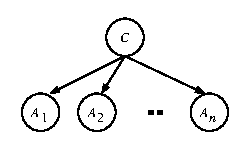
\includegraphics[scale=1.3]{fig/nbayes.eps}}
\caption{Bayesian network representation of a naive Bayes model.}
\label{fig:nbayes}
\end{figure}

\section{$n$-fold cross validation of a naive Bayes classifier}
\label{sec:example:cv}

The main goal in version 1.12 was to add facilities for ease of programming,
and under this goal, dozens of built-in predicates for randomization, statistical
operations and list processing were introduced to the programming system
(see \secref{sec:built-in:random}, \secref{sec:built-in:measure} and
\secref{sec:built-in:list}, respectively).  To demonstrate the usefulness of
these built-ins, in this section, we try to write a compact evaluation routine
of a naive Bayes classifier~\cite{Mitchell97}\conindex{naive Bayes classifier}
based on $n$-fold cross validation.\conindex{cross validation}

A naive Bayes classifier is a probabilistic classifier based on a naive Bayes
model, a special form of a Bayesian network (see Figure~\ref{fig:nbayes}).  First,
the attribute values $\langle a_1,a_2,\ldots,a_m\rangle$ of an example are
considered as a realization of a random vector $\langle A_1,A_2,\ldots,A_m\rangle$,
and also the class $c$ to which the example belongs is a realization of a random variable
$C$.  Then, in naive Bayes models, the joint probability distribution is simplified
under the conditional independence among attributes:
\[
P(c,a_1,a_2,\ldots,a_m)=P(c)\prod_{j=1}^m P(a_j\mid c),
\]
where we abbreviate $P(A_j=a_j,\ldots)$ as $P(a_j,\ldots)$, and $P(C=c,\ldots)$
as $P(c,\ldots)$.
After the probabilities $P(c)$ and $P(a_j\mid c)$ estimated from training examples,
we get the most probable class $c^\ast$ for a test example having
$\langle a_1,a_2,\ldots,a_m\rangle$ by:
\begin{eqnarray}
c^\ast
&=&\argmax_c P(c\mid a_1,a_2,\ldots,a_m)\nonumber\\
&=&\argmax_c P(c,a_1,a_2,\ldots,a_m)\nonumber\\
&=&\argmax_c P(c)\prod_{j=1}^m P(a_j\mid c).\label{eq:nbayes:predict}
\end{eqnarray}

To conduct an $n$-fold cross validation\conindex{cross validation} for a naive Bayes classifier,
we have at least five types of tasks:\ (1) estimation of the probabilities $P(c)$ and $P(a_j\mid c)$
from training examples, (2) computation of the most probable class $c^\ast$, (3) rotated splitting
of the whole dataset into training examples and test examples, (4) computation of predictive
accuracy, and (5) iteration of the tasks (1)--(4) for $n$ times.  Using the
built-ins for EM learning and Viterbi computation, we can realize the tasks (1) and (2),
respectively.  For the task~(3), new built-in predicates for shuffling and splitting lists
can be used.  The task~(4) will be easily implemented by a new built-in predicate for average
operation.  Finally, to realize the loops for the task~(5) compactly, we use
map functions\conindex{map function} instead of recursive predicates.

Now let us see the program.  The target is the congressional voting records dataset,
\exindex{congressional voting records dataset} which is available from
UCI machine learning repository\exindex{UCI machine learning repository}
({\tt http://\lb archive.\lb ics.\lb uci.\lb edu/\lb ml/}).
We suppose that the data file {\tt house-votes-84.data} has been downloaded and
is placed `as is' under the current directory.  First of all, we declare random switches:
%
\begin{quote}
\begin{verbatim}
values(class,[democrat,republican]).
values(attr(_,_),[y,n]).
\end{verbatim}
\end{quote}
%
The random switch {\tt class} takes two values that indicate the class labels {\tt democrat}
and {\tt republican}.  The probabilities $P(c)$ correspond to $\theta_{{\tt class},c}$, the
parameters of a random switch {\tt class} ($c = \mathtt{democrat}$, $\mathtt{republican}$).
On the other hand, since all attributes only take `{\tt y}' or `{\tt n}' (here `{\tt ?}'
is treated as a missing value\footnote{
The data description file {\tt house-votes-84.names}, also downloadable from the repository,
contains a warning --- {\it It is important to recognize that ``?'' in this database does not
mean that the value of the attribute is unknown.  It means simply, that the value is not
``yea'' or ``nay'' (\ldots).}  In this section, on the other hand, we consider `{\tt ?}'
as a missing value just for demonstration.
}), all random switches named {\tt attr($j$,$c$)} also take on values `{\tt y}' and `{\tt n}'.
The probabilities $P(a_j\mid c)$ correspond to $\theta_{{\tt attr}(j,c),a_j}$ ($j=1,\ldots,m$).

The modeling part only includes four clauses.  Since a naive Bayes model is a special form
of a Bayesian network, the programming is basically done in the manner described in
\secref{sec:example:bn}:
%
\progindex{nbayes/2}
\progindex{nbayes/3}
\progindex{choose/3}
\begin{quote}
\begin{verbatim}
nbayes(C,Vals):- msw(class,C),nbayes(1,C,Vals).

nbayes(_,_,[]).
nbayes(J,C,[V|Vals]):-
    choose(J,C,V),
    J1 is J+1,
    nbayes(J1,C,Vals).


choose(J,C,V):- 
    ( V == '?' -> msw(attr(J,C),_)
    ; msw(attr(J,C),V)
    ).
\end{verbatim}
\end{quote}
%
In this program, the logical variables {\tt C} and {\tt Vals} in {\tt nbayes(C,Vals)}
correspond to the random variable $C$ and the random vector $\langle A_1,A_2,\ldots,A_m\rangle$.
Also, instead of calling {\tt msw(attr(J,C),V)} directly, we use a wrapper {\tt choose(J,C,V)}
which has an additional if-then branch for handling missing values.

Let us move to the utility part,\conindex{utility part} which includes evaluation routines.
First, we can conduct an {\tt N}-fold cross validation by running the top predicate
{\tt votes\_cv(N)}:
\progindex{votes\_cv/1}
\begin{small}
\begin{verbatim}
votes_cv(N):-
    random_set_seed(81729), % Fix the random seed to keep the same splitting
    load_data_file(Gs0),    % Load the entire data
    random_shuffle(Gs0,Gs), % Randomly reorder the data
    numlist(1,N,Ks),        % Get Ks = [1,...,N] (B-Prolog built-in)
    maplist(K,Rate,votes_cv(Gs,K,N,Rate),Ks,Rates),
                            % Call votes_cv/2 for K=1...N
    avglist(Rates,AvgRate), % Get the avg. of the precisions
    maplist(K,Rate,format("Test #~d: ~2f%~n",[K,Rate*100]),Ks,Rates),
    format("Average: ~2f%~n",[AvgRate*100]).
\end{verbatim}
\end{small}
Please see the comments to understand the behavior. {\tt load\_data\_file(Gs0)}
reads the whole dataset from {\tt house-votes-84.data} and returns a list of
{\tt nbayes(C,Vals)} to {\tt Gs0} (the definition will be given later).  The examples
{\tt Gs0} are shuffled into {\tt Gs} by {\tt random\_shuffle/2}, a built-in
predicate newly introduced in version 1.12.  The first call of {\tt maplist/5}
invokes {\tt votes\_cv(Gs,\lb K,N,Rate)} for each {\tt K} in {\tt Ks} =
{\tt [1,\ldots,N]}, and stores its output {\tt Rate} into a list {\tt Rates}.
Here {\tt votes\_cv(Gs,\lb K,N,Rate)} takes as input {\tt Gs}, {\tt K}
and {\tt N}, and returns the predictive accuracy {\tt Rate} for the {\tt K}-th
splitting.  We finally get the average predictive accuracy {\tt AvgRate} by
{\tt avglist(Rates,AvgRate)}, a built-in for average operation.
It is important to note that, by using {\tt maplist/5}, we can often avoid writing
a definition of the recursive clause representing a loop for {\tt K}, and keep
the program compact.

The predicate {\tt votes\_cv(Gs,K,N,Rate)}, which we have seen above, works
on EM learning and Viterbi computation for the {\tt K}-th splitting:
\progindex{votes\_cv/4}
\begin{small}
\begin{verbatim}
votes_cv(Gs,K,N,Rate):-
    format("<<<< Test #~d >>>>~n",[K]),
    separate_data(Gs,K,N,Gs0,Gs1),  % Gs0: training data, Gs1: test data
    learn(Gs0),                     % Learn by PRISM's built-in
    maplist(nbayes(C,Vs),R,(viterbig(nbayes(C0,Vs)),(C0==C->R=1;R=0)),Gs1,Rs),
                       % Predict the class by viterbig/1 for each test example
                       %           and evaluate it with the answer class label
    avglist(Rs,Rate),  % Get the accuracy for the K-th splitting
    format("Done (~2f%).~n~n",[Rate*100]).
\end{verbatim}
\end{small}
In the clause body, {\tt separate\_data(Gs,K,N,Gs0,Gs1)} splits the whole dataset
{\tt Gs} into training examples {\tt Gs0} and test examples {\tt Gs1}.  We train
the naive Bayes model in a usual manner by {\tt learn/1} and make predictions
for test examples one by one using {\tt viterbig/1}.  Here we use {\tt maplist/5}
again for repeated testings.  Furthermore, the predicted classes are evaluated
with the answer class labels, and the evaluation results will be stored as a list
of {\tt 1} (correct) and {\tt 0} (incorrect).  Lastly, by interpreting these
{\tt 1}s and {\tt 0}s numerically and taking their average, we get the
predictive accuracy as {\tt Rate}.

The remaining predicates are defined as follows:
\progindex{separate\_data/2}
\progindex{load\_data\_file/1}
\begin{small}
\begin{verbatim}
separate_data(Data,K,N,Learn,Test):-
    length(Data,L),
    L0 is L*(K-1)//N,    % L0: offset of the test data (// - integer division)
    L1 is L*(K-0)//N-L0, % L1: size of the test data
    splitlist(Learn0,Rest,Data,L0),   % Length of Learn0 = L0
    splitlist(Test,Learn1,Rest,L1),   % Length of Test = L1
    append(Learn0,Learn1,Learn).

load_data_file(Gs):-
    load_csv('house-votes-84.data',Gs0),
    maplist(csvrow([C|Vs]),nbayes(C,Vs),true,Gs0,Gs).
\end{verbatim}
\end{small}
In the definition of {\tt separate\_data/5}, we use {\tt splitlist/4}, a new
built-in for splitting lists.  Another user predicate {\tt load\_data\_file/1}
uses {\tt load\_csv/2} to read a CSV file ({\tt house-votes-84.data}) directly
and {\tt maplist/5} to convert each row in the CSV file into an observed goal
{\tt nbayes(C,Vs)} in the model.

It has been claimed that one advantage of PRISM programming is the compactness
of the modeling part.  Besides, as we have seen, with the built-ins introduced in
version 1.12, we can make the utility part compact as well.  It is also interesting
to see that we can write a routine for $n$-fold cross validation just by combining
general-purpose built-in predicates.  Now let us run the program:
\progindex{votes\_cv/1}
\begin{small}
\begin{quote}
\begin{verbatim}
% prism
  :
?- prism(votes).
  :
?- votes_cv(10).

<<<< Test #1 >>>>
#goals: 0.........100.........200.........300.(312)
Exporting switch information to the EM routine ... done
#em-iters: 0(8) (Converged: -3076.540683710)
Statistics on learning:
        Graph size: 6284
        Number of switches: 33
        Number of switch instances: 66
        Number of iterations: 8
        Final log likelihood: -3076.540683710
        Total learning time: 0.024 seconds
        Explanation search time: 0.016 seconds
        Total table space used: 1671056 bytes
Type show_sw or show_sw_b to show the probability distributions.
Done (81.40%).

  :

<<<< Test #10 >>>>
#goals: 0.........100.........200.........300.(311)
Exporting switch information to the EM routine ... done
#em-iters: 0(8) (Converged: -3134.945195139)
Statistics on learning:
        Graph size: 6260
        Number of switches: 33
        Number of switch instances: 66
        Number of iterations: 8
        Final log likelihood: -3134.945195139
        Total learning time: 0.028 seconds
        Explanation search time: 0.016 seconds
        Total table space used: 1663976 bytes
Type show_sw or show_sw_b to show the probability distributions.
Done (90.91%).

Test #1: 81.40%
Test #2: 88.64%
Test #3: 90.70%
Test #4: 93.18%
  :
Test #9: 95.35%
Test #10: 90.91%
Average: 90.11%

yes
\end{verbatim}
\end{quote}
\end{small}


\section{Dieting professor*}
\label{sec:example:chmm}
\exindex{dieting professor program|(}

The last example is a program that deals with failures
\conindex{failure (in the generation process)}
in the generation process\conindex{generation process}.  Let us consider
a scenario as follows. There is a professor who takes a lunch everyday at
one of two restaurants `{\tt s0}' and `{\tt s1}', and he changes the
restaurant to visit probabilistically.  Also as he is on a diet,
he needs to satisfy a {\em constraint}\conindex{constraint} that
the total calories for lunch in a week are less than 4K calories.
He probabilistically orders pizza (which is denoted by `{\tt p}'
and has 900 calories) or sandwich (`{\tt s}'; 400 calories)
at the restaurant `{\tt s0}', and hamburger (`{\tt h}'; 400 calories)
or sandwich (`{\tt s}'; 500 calories) at the restaurant `{\tt s1}'.
He records what he has eaten like {\tt [p,s,s,p,h,s,h]} in a week
and he preserves the  record {\em only if} he succeeds in keeping
the constraint.  For example, we have a list of preserved records,
and attempt to estimate the probability that he violates the constraint.

\begin{figure}[t]
\centerline{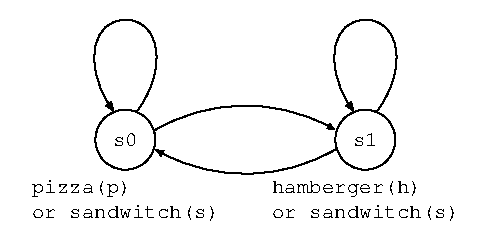
\includegraphics[scale=1.0]{fig/chmm.eps}}
\caption{State transition diagram of the dieting professor.}
\label{fig:chmm}
\end{figure}

First of all, let us introduce a two-state hidden Markov model
(HMM),\conindex{hidden Markov model}
shown in Figure~\ref{fig:chmm}, as a basic model that
captures the professor's probabilistic behavior.  We then try
to write a PRISM program which represents this basic model
with the additional constraint on the total calories.
Hereafter we call the model a {\em constrained HMM}.
\exindex{HMM program!constrained ---}
Let us describe the program.  From Figure~\ref{fig:chmm}, we can
see that four switches are required as follows:

\predindex{values/2}
\begin{quote}
\begin{verbatim}
values(tr(s0),[s0,s1]).
values(tr(s1),[s1,s0]).
values(lunch(s0),[p,s]).  % pizza:900,  sandwich:400
values(lunch(s1),[h,s]).  % hamburger:400, sandwich:500
\end{verbatim}
\end{quote}

\noindent
where the switches named {\tt tr($\cdot$)} choose the next restaurant,
and those named {\tt lunch($\cdot$)} select the menu of lunch
at the chosen restaurant.

The central part of the model is {\tt chmm/4}, which is defined as follows:
\conindex{modeling part}
\begin{quote}
\begin{verbatim}
chmm(L,S,C,N):- N>0,
  msw(tr(S),S2),
  msw(lunch(S),D),
  ( S == s0,
     ( D = p, C2 is C+900
     ; D = s, C2 is C+400 )
  ; S == s1,
     ( D = h, C2 is C+400
     ; D = s, C2 is C+500 )
  ),
  L=[D|L2],
  N2 is N-1,
  chmm(L2,S2,C2,N2).
chmm([],_,C,0):- C < 4000.
\end{verbatim}
\end{quote}

\noindent
This predicate behaves similarly to {\tt hmm/3} (\secref{sec:example:hmm}),
a recursive routine, except that {\tt chmm/4} has an additional argument
that accumulates the total calories in a week.  It is important
to notice here that, when the recursion terminates, the total calories
will be checked in the second clause, and if the total calories violate
the constraint, the predicate {\tt chmm/4} totally fails.  This corresponds
to the scenario that the professor only preserves the record only if
he succeeds to keep the constraint.\conindex{constraint}

To learn the parameters from his records, or to know the probability that
he fails to keep the constraint, we need to make further settings.
For example, we may define the four predicates as follows:

\predindex{failure/0}
\progindex{failure/1}
\progindex{success/0}
\progindex{success/1}
\begin{quote}
\begin{verbatim}
failure:- not(success).
success:- success(_).
success(L):- chmm(L,s0,0,7).
failure(L):- not(success(L)).
\end{verbatim}
\end{quote}

\noindent
From the definition of {\tt chmm/4}, {\tt success($L$)}\progindex{success/1}
says that the professor succeeds to keep the constraint with the menus $L$.
So {\tt success/0}\progindex{success/0} indicates the fact that he succeeds
to keep the constraint.  {\tt failure/0}\predindex{failure/0} is the negation
of {\tt success/0} and therefore means that he fails to satisfy the constraint.
{\tt failure($L$)}\progindex{failure/1} is optional here but says that he
fails to keep the constraint due to the menus $L$.

\noindent
We consider the predicates {\tt success/1} and {\tt failure/0} as
observable predicates, and we use {\tt learn/1} as a learning command.

The experiment we attempt is artificial, similarly to those with HMMs
(\secref{sec:example:hmm}) and discrete Bayesian networks (\secref{sec:example:bn})
--- we first generate samples under the predefined parameters,
and then learn the parameters\conindex{parameter learning}
from the generated samples.  For this experiment, we define
a predicate in the utility part,\conindex{utility part}
that specifies some predefined parameters:

\predindex{set\_sw/2}
\predindex{sample/1}
\begin{quote}
\begin{verbatim}
set_params:-
  set_sw(tr(s0),[0.7,0.3]),
  set_sw(tr(s1),[0.7,0.3]),
  set_sw(lunch(s0),[0.4,0.6]),
  set_sw(lunch(s1),[0.5,0.5]).
\end{verbatim}
\end{quote}

Now we are in a position to start the experiment.  We first load
the program with the built-in {\tt prismn/1} (please note `{\tt n}'
at the last of the predicate name):

\predindex{prismn/1}
\begin{quote}
\begin{small}
\begin{verbatim}
?- prismn(chmm).

step1.
step2.
step3.
Compilation done by FOC

compiled in 12 milliseconds
loading::temp.out

yes
\end{verbatim}
\end{small}
\end{quote}

\noindent
Let us recall that the definition clauses of {\tt failure/0}\predindex{failure/0}
and {\tt failure/1} have negation {\tt not/1}\predindex{not/1} in their bodies.
This is not negation as failure\conindex{negation as failure} (NAF),
and we need a special treatment for such negation.
{\tt prismn/1} calls an implementation of First Order
Compiler\conindex{First Order Compiler} (FOC)~\cite{Sato89} to
eliminate negation {\tt not/1}.  In the messages above, the messages
from ``{\tt step1}'' to ``{\tt Compilation done by FOC}'' are produced by
the FOC routine, and we may notice that the predicates whose names start
with `{\tt closure\_}' are newly created by the FOC routine and
registered as table predicates (because they are probabilistic).

After loading, we set the parameters by {\tt set\_params/0},
and confirm the specified parameters:

\predindex{show\_sw/0}
\begin{quote}
\begin{verbatim}
?- set_params,show_sw.

Switch lunch(s0): unfixed_p: p (p: 0.400000000) s (p: 0.600000000)
Switch lunch(s1): unfixed_p: h (p: 0.500000000) s (p: 0.500000000)
Switch tr(s0): unfixed_p: s0 (p: 0.700000000) s1 (p: 0.300000000)
Switch tr(s1): unfixed_p: s1 (p: 0.700000000) s0 (p: 0.300000000)
\end{verbatim}
\end{quote}

\noindent
We can compute the probability that the professor fails to keep the
constraint under the parameters above:

\predindex{prob/1}
\begin{quote}
\begin{verbatim}
?- prob(failure).
Probability of failure is: 0.348592596784000
\end{verbatim}
\end{quote}

\noindent
From this, we can say that the professor skips preserving the record
once in three weeks.

To make it sure that the program correctly represents our model
(in particular, the definition of the {\tt failure} predicate),
we may give a couple of queries.  For example, the following query
confirms whether the sum of the probability that the professor
satisfy the constraint and the probability that he does not
becomes unity:\footnote{
Unfortunately, as shown here, the actual result of the sum will not always
be unity for precision errors.
}

\predindex{prob/2}
\begin{quote}
\begin{verbatim}
?- prob(success,Ps),prob(failure,Pf),X is Ps+Pf.

Pf = 0.348592596784
Ps = 0.651407403215999
X = 0.999999999999998 ?
\end{verbatim}
\end{quote}

\noindent
Or we have a similar query which is limited to some specific
menu (obtained as {\tt L} by sampling):

\predindex{sample/1}
\predindex{prob/2}
\begin{quote}
\begin{verbatim}
?- sample(success(L)),
   prob(success(L),Ps),prob(failure(L),Pf),
   X is Ps+Pf.

Pf = 0.9999321868
Ps = 0.0000678132
L = [s,p,h,s,h,p,h]
X = 1.0 ?
\end{verbatim}
\end{quote}

\noindent
It is confirmed for each goal appearing in the queries above that the sum
of probabilities of the goal and its negation is always unity, so we can
proceed to a learning experiment.  To conduct it, we use the built-in
{\tt get\_samples\_c/4}\predindex{get\_samples\_c/4}
to generate 500 samples (note that we cannot simply use {\tt get\_samples/3}
\predindex{get\_samples/3} since a sampling of {\tt success(L)} may fail),
and invoke the learning command with the samples:

\predindex{learn/1}
\begin{quote}
\begin{small}
\begin{verbatim}
?- get_samples_c([inf,500],success(L),true,Gs),learn([failure|Gs]).

sampling -- #success = 500
sampling -- #failure = 249
#goals: 0.........100.........200......(266)
Exporting switch information to the EM routine ...
#em-iters: 0........(83) (Converged: -2964.788301553)
Statistics on learning:
        Graph size: 9328
        Number of switches: 4
        Number of switch instances: 8
        Number of iterations: 83
        Final log likelihood: -2964.788301553
        Total learning time: 0.036 seconds
        Explanation search time: 0.016 seconds
        Total table space used: 1486208 bytes
Type show_sw or show_sw_b to show the probability distributions.
Gs = [success([s,s,s,h,s,h,h]),success([s,p,h,s,h,h,s]),
      ... omitted ...
      success([s,p,h,h,s,p,s]),success([p,s,s,s,h,s,s])] ?
yes
\end{verbatim}
\end{small}
\end{quote}

\noindent
It should be noted that, if a special symbol {\tt failure}\index{predicate}{failure@{\tt failure} (Prolog atom used in {\tt learn/1})}
is included to the goals in {\tt learn/1}, the EM algorithm considering
failure\conindex{expectation-maximization algorithm}
\conindex{failure (in the generation process)}
called the failure-adjusted maximization (FAM) algorithm
\conindex{failure-adjusted maximization algorithm}
will be invoked.  After learning, we can confirm the
learned parameters as usual:

\predindex{show\_sw/0}
\begin{quote}
\begin{small}
\begin{verbatim}
?- show_sw.

Switch lunch(s0): unfixed_p: p (p: 0.380041828) s (p: 0.619958172)
Switch lunch(s1): unfixed_p: h (p: 0.537922906) s (p: 0.462077094)
Switch tr(s0): unfixed_p: s0 (p: 0.714988121) s1 (p: 0.285011879)
Switch tr(s1): unfixed_p: s1 (p: 0.677016948) s0 (p: 0.322983052)
\end{verbatim}
\end{small}
\end{quote}

\exindex{dieting professor program|)}

\section{Linear-chain CRFs*}
\label{sec:example:crf}

\exindex{linear-chain CRF program|(}

Linear-chain CRFs\conindex{conditional random fields!linear-chain ---}
are well-known  discriminative models for sequence data used
in natural language processing, image processing, bioinformatics and so on.
Their  generative counter  part is  HMMs which  form generative-discriminative
pairs with linear-chain  CRFs.  Here we define a simple  linear-chain CRF as a
generative CRF\conindex{generative conditional random fields}
by  our approach.  So we begin by writing  code for a two-place
predicate {\tt  hmm0/2} that  specifies an HMM  program for complete  data and
then write specialized code for  a one-place predicate {\tt hmm0/1} to compute
the marginalized unnormalized distribution.

The PRISM program below represents a linear-chain  CRF with two
states, {\tt s0}  and {\tt s1}, and  two output symbols, {\tt a}  and {\tt b}.
Two  predicates,  {\tt hmm0/2}  and  {\tt  hmm0/1},  are defined  there.   The
two-place predicate  {\tt hmm0(Xs,Ys)} specifies generatively  a complete data
consisting of  two sequences, a  sequence {\tt Xs}  of output symbols  and the
corresponding  sequence {\tt  Ys} of  hidden states.   Likewise  the one-place
predicate {\tt hmm0(Xs)} specifies a usual  HMM where ${\tt Xs}$ is a sequence
of observed  symbols.  Note  that these predicates  have isomorphic  code and
once {\tt hmm0/2} is encoded, it  is relatively easy to encode {\tt hmm0/1} as
their codes are isomorphic.

% Two-state CRF-HMM
% N.B.: hmm0/1 defines an HMM but the code differs from
% the HMM example included in the distributed package.
\begin{quote}
\begin{small}
\begin{verbatim}
values(init,[s0,s1]).
values(tr(_),[s0,s1]).
values(out(_),[a,b]).

hmm0([X0|Xs],[Y0|Ys]):-     % for unnormalized distribution
   msw(init,Y0),msw(out(Y0),X0),hmm1(Y0,Xs,Ys).
hmm1(_,[],[]).
hmm1(Y0,[X|Xs],[Y|Ys]):-
   msw(tr(Y0),Y),msw(out(Y),X),hmm1(Y,Xs,Ys).

hmm0([X|Xs]):-              % for marginalized unnormalized distribution
   msw(init,Y0),msw(out(Y0),X),hmm1(Y0,Xs).
hmm1(_,[]).
hmm1(Y0,[X|Xs]):-
   msw(tr(Y0),Y1),msw(out(Y1),X),hmm1(Y1,Xs).
\end{verbatim}
\end{small}
\end{quote}

Now let  us test weight learning  using {\tt crf\_learn/1}.\footnote{
  When the PRISM system runs {\tt crf\_learn/1} for a complete dataset, say {\tt
    r($x_1$,$y_1$)},\ldots,{\tt r($x_T$,$x_T$)}, it searches the program for the
  companion predicate {\tt r(X)} and its defining clauses as well as clauses for
  {\tt r(X,Y)} to compute the marginalized unnormalized distribution.
}
We first set  flags for learning. Then we draw a  sample {\tt \_Gs} of size
50 from {\tt hmm0(Xs,Ys)}\footnote{
  Sampling  is possible  because at  the point  of running  {\tt get\_samples/3}
  command, the  switch database  holds (default) probabilities.   However, after
  running {\tt crf\_learn/1}, probabilities are replaced by weights and sampling
  is (usually)  impossible.  Sampling becomes  possible again if {\tt  msw}s are
  reset              for               example              by
  {\tt ?- set\_prism\_flag(default\_sw,uniform), set\_sw\_all.}
}
such  that  the  length  of  {\tt  Xs}  and  {\tt  Ys}  is  five  using  {\tt
  get\_samples/3}     and     learn      the     weights     $\vlambda$     in
Eq.~\ref{eq:regcondlikelihood} by {\tt crf\_learn(\_Gs)} from the sample.

% In the example use below, reset_param/0 resets weights of msws and
% get_samples/3 generates a random sample of size 50
% of complete data using hmm0/2.
%
% Example use:
% ?- prism(crf_hmm)
% ?- set_prism_flag(crf_learn_mode,fg)
% ?- set_prism_flag(crf_learning_rate,golden)
% ?- set_prism_flag(log_scale,off).

\flagindex{crf\_penalty}
\flagindex{crf\_learn\_mode}
\predindex{crf\_learn/1}
\begin{quote}
\begin{small}
\begin{verbatim}
?- set_prism_flag(crf_penalty,1.0).
?- set_prism_flag(crf_learn_mode,lbfgs).
?- get_samples(50,hmm0(Xs,[_,_,_,_,_]),_Gs), crf_learn(_Gs).

#goals: 0.......(72)
Exporting switch information to the CRF-learn routine ... done
L-BFGS mode
#crf-iters: 0.......(79) (Converged: -168.571830502)
Statistics on learning:
        Graph size: 987
        Number of switches: 5
        Number of switch instances: 10
        Number of iterations: 79
        Final log likelihood: -168.571830502
        Total learning time: 0.007 seconds
        Explanation search time: 0.002 seconds
        Total table space used: 97696 bytes
Type show_sw to show the lambdas.
\end{verbatim}
\end{small}
\end{quote}

\noindent
After learning, we print out the switch database to see learned weights
($\vlambda$ in Eq.~\ref{eq:regcondlikelihood}).
%
\predindex{show\_sw/0}
\begin{quote}
\begin{small}
\begin{verbatim}
?- show_sw
Switch init: unfixed_p: s0 (p: 0.149259244) s1 (p: -0.149259244)
Switch out(s0): unfixed_p: a (p: 0.159373024) b (p: 0.058738941)
Switch out(s1): unfixed_p: a (p: -0.159373024) b (p: -0.058738941)
Switch tr(s0): unfixed_p: s0 (p: -0.064599964) s1 (p: -0.337089215)
Switch tr(s1): unfixed_p: s0 (p: 0.133452685) s1 (p: 0.268236494)
\end{verbatim}
\end{small}
\end{quote}

%-------------
% fprob family
% 
% Comment:
% This family computes weights of goals.
% fprob(G) computes the weight of a goal G and displays it.
% fprobf(G) is identical to probf(G) and prints out an explanation graph.
% fprobfi(G) displays an explanation graph with weights.
% fprob(G,W), fprobf(G,EG) and fprobfi(G,EG) are longer versions of
% fprobf/1, fprobf/1 and fprobfi/1 respectively. They
% return, depending on the predicate, the weight W of G or
% an explanation graph EG for G.
%
% Example use:
% ?- prism(crf_hmm).
% ?- fprob(hmm0([a,b,b])).
% ?- fprobf(hmm0([a,b,b])).
% ?- fprobfi(hmm0([a,b,b])).
% ?- fprob(hmm0([a,b,b]),W).
% ?- fprobf(hmm0([a,b,b]),EG)
% ?- fprobfi(hmm0([a,b,b]),EG)

\noindent
Next we compute the weight {\tt W} of {\tt hmm0([a,b,b])}.
%
\flagindex{log\_scale}
\predindex{crf\_prob/1}
\begin{quote}
\begin{small}
\begin{verbatim}
?- set_prism_flag(log_scale,off).
?- crf_prob(hmm0([a,b,b]),W).

W = 8.42869
\end{verbatim}
\end{small}
\end{quote}

%-------------
% crf_hindsight family
%
% Comment:
% This family performs hindsight computation for CRFs.
% crf_hindsight(G), crf_hindsight(G,SubG) and crf_hindsight(G,SubG,SubGWs)
% exactly behave like the correpsonding non-crf predicates, i.e.,
% hindsight(G), hindsight(G,SubG) and hindsight(G,SubG,HProbs) respectively,
% but use weights instead of probabilities in hindsight computation.
%
% Example use:
% ?- prism(crf_hmm).
% ?- crf_hindsight(hmm0([a,b,b])).
% ?- crf_hindsight(hmm0([a,b,b]),hmm1(s1,_)).
% ?- crf_hindsight(hmm0([a,b,b]),hmm1(s1,_),SubGWs).


%-------------
% crf_viterbi family
%
% Comment:
% This family carries out a variety of Viterbi inference
% (computing the best explanation) for CRFs.
% The basic Viterbi predicates, i.e.,
% crf_viterbi(G), crf_viterbi(G,W), crf_viterbif(G) and  crf_viterbif(G,W,EG)
% are just crf-versions of the corresponding non-crf viterbi predicates
% which use weights instead of probabilities.
% So crf_viterbif(G,W,EG) returns the weight of G and the most probable explanation
% EG for G and so on.
% 
% Example use:
% ?- prism(crf_hmm).
% ?- crf_viterbi(hmm0([a,b,b])).
% ?- crf_viterbi(hmm0([a,b,b]),W).
% ?- crf_viterbif(hmm0([a,b,b])).
% ?- crf_viterbif(hmm0([a,b,b]),W,EG).

\noindent
We further print out the Viterbi  explanation and its weight for the same goal
using {\tt crf\_viterbi/1}.
%
\predindex{crf\_viterbi/1}
\begin{quote}
\begin{small}
\begin{verbatim}
?- crf_viterbif(hmm0([a,b,b]))
hmm0([a,b,b])
   <= hmm1(s0,[b,b]) & msw(init,s0) & msw(out(s0),a)
hmm1(s0,[b,b])
   <= hmm1(s0,[b]) & msw(tr(s0),s0) & msw(out(s0),b)
hmm1(s0,[b])
   <= hmm1(s0,[]) & msw(tr(s0),s0) & msw(out(s0),b)
hmm1(s0,[])

CRF-Viterbi_P = 0.445365332417886
\end{verbatim}
\end{small}
\end{quote}

% The viterbig subfamiliy, i.e., crf_viterbig(G), crf_viterbig(G,W) and crf_viterbig(G,W,V),
% are non-crf versions of the corresponding viterbig predicates.
% crf_viterbig(G,W,EG) instantiates G to a ground goal G' with most probable values for the variables in G
% and returns the weight W of G' and the most probable expiation graph EG for G'.
% crf_viterbig(G,W) = crf_viterbig(G,W,_) and crf_viterbig(G) returns answer substitutions.
% 
% Example use:
% ?- prism(crf_hmm).
% ?- crf_viterbig(hmm0([X,b,Y])).
% ?- crf_viterbig(hmm0([X,b,Y]),W).
% ?- crf_viterbig(hmm0([X,b,Y]),W,EG).

\noindent
Of course,  we are  able to know  the most probable instantiation and  the most
probable top-$n$ instantiations as follows  using {\tt crf\_viterbig/1}
and {\tt n\_crf\_viterbig/2} respectively.\footnote{
  {\tt n\_crf\_viterbig/2} is a backtrackable predicate.
}.
%
\predindex{crf\_viterbig/1}
\predindex{n\_crf\_viterbig/2}
\begin{quote}
\begin{small}
\begin{verbatim}
?- crf_viterbig(hmm0([X,b,Y])).
X = a
Y = a

?- bagof([X,Y],n_crf_viterbig(3,hmm0([X,b,Y])),Zs).
Zs = [[a,a],[a,b],[b,a]]
\end{verbatim}
\end{small}
\end{quote}

% The viterbit subfamiliy, i.e., crf_viterbit(G) and crf_viterbit(G,W,T),
% computes a Viterbi explanation T for G in a tree form.
% crf_viterbit(G) displays T whereas crf_viterbit(G,W,T) returns
% the weight W of G and T.
%
% Example use:
% ?- prism(crf_hmm).
% ?- crf_viterbit(hmm0([a,b,b])).
% ?- crf_viterbit(hmm0([a,b,b]),W,T).

%-------------
% n_crf_viterbi family
%
% Comment:
% Predicates in this family have the form n_crf_viterbi..(N,...) and
% compute N best explanations for a CRF in various styles.
% When N=1, they are reduced to the corresponding predicates
% crf_viterbi..(N,...) in the crf_viterbi family.
% So their use is basically the same as the crf_viterbi family but
% needs N as the first argument.
% Basic predicates are n_crf_viterbi(N,G), n_crf_viterbi(N,G,Ws),
% n_crf_viterbif(N,G) and n_crf_viterbif(N,G,VEs).
% They compute N best explanations for a goal G together with,
% depending on the predicate, their weights Ws and explanations VEs.
% Note that VEs, viterbi explanations, have different form from
% usual explanation graphs.
%
% Example use:
% ?- prism(crf_hmm).
% ?- n_crf_viterbi(3,hmm0([a,b,b])).
% ?- n_crf_viterbi(3,hmm0([a,b,b]),Ws).
% ?- n_crf_viterbif(3,hmm0([a,b,b])).
% ?- n_crf_viterbif(3,hmm0([a,b,b]),VEs).

% n_crf_viterbig(N,G), n_crf_viterbig(N,G,W) and n_crf_viterbig(N,G,W,EG)
% compute N best explanations for a goal G while ground-instantiating G.
% They are backtrackable. So for example n_crf_viterbig(N,G) returns
% answer substitutions for G one by one by backtracking
% up to N substitutions.
%
% Example use:
% ?- prism(crf_hmm).
% ?- n_crf_viterbig(3,hmm0([a,b,Y])).
% ?- bagof(Y,n_crf_viterbig(3,hmm0([a,b,Y])),Ys).
% ?- bagof([Y,W],n_crf_viterbig(3,hmm0([a,b,Y]),W),Z).
% ?- bagof([Y,W,EG],n_crf_viterbig(3,hmm0([a,b,Y]),W,EG),Z).

% n_crf_viterbit(N,G) and n_crf_viterbit(N,G,Ts) compute N best
% explanations in a tree form.
% n_crf_viterbit(N,G) display them and n_crf_viterbit(N,G,Ts)
% returns them in Ts.
% 
% Example use:
% ?- prism(crf_hmm).
% ?- n_crf_viterbit(3,hmm0([a,b,b])).
% ?- n_crf_viterbit(3,hmm0([a,b,b]),Ts).

\exindex{linear-chain CRF program|)}

\section{Linear cyclic explanation graph*}
\label{sec:example:lin}

\exindex{discrete time Markov chain program|(}

Cyclic  explanation graphs (Chapter~\ref{chap:cycle})
enable us  to deal  with useful  models  of cyclic
probabilistic  relations.  For  example, a  reachability relation  in discrete
time Markov chains\conindex{discrete time Markov chains}
and infinite recursion associated with the computation of
prefix probability\conindex{prefix probability} in PCFGs yield
cyclic explanation graphs~\cite{Sato13}.
%  It is possible to compute their probabilities easily by the PRISM system.

\begin{figure}[t]
  \begin{center}
    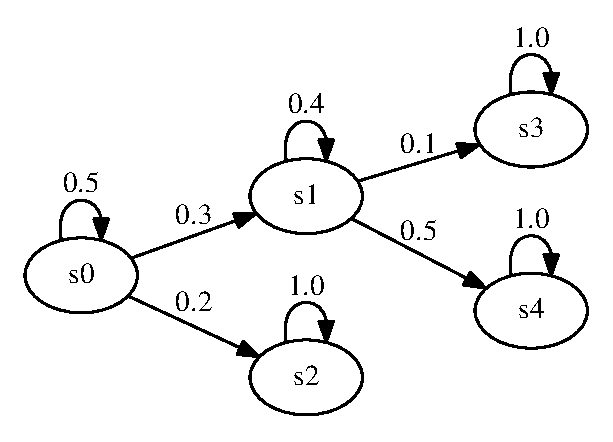
\includegraphics[width=0.4\hsize]{fig/DTMC01.eps}
    \caption{An example of discrete time Markov chains}
    \label{fig:dtmc}
  \end{center}
\end{figure}

To  have a  close look  at cyclic  explanation graphs,  we introduce  a sample
program that  describes the  reachability relation on  a discrete  time Markov
chain shown in Figure~\ref{fig:dtmc}, where a state transition is made
by a probabilistic choice of next state by {\tt msw/2}:
%
\flagindex{error\_on\_cycle}
\begin{quote}
\begin{small}
\begin{verbatim}
:- set_prism_flag(error_on_cycle,off).

values(t(s0),[s0,s1,s2],[0.5,0.3,0.2]).
values(t(s1),[s1,s3,s4],[0.4,0.1,0.5]).
values(t(s2),[s2],[1.0]).
values(t(s3),[s3],[1.0]).
values(t(s4),[s4],[1.0]).

tr(S,T) :- get_values(t(S),OS),member(T,OS),msw(t(S),T).
reach(S,S).
reach(S,T) :- \+S==T,tr(S,U),reach(U,T).
\end{verbatim}
\end{small}
\end{quote}
%
Since   this   Markov   chain   has   a  self-loop   at   each   state,   {\tt
probf(reach(s0,s3))} returns a cyclic explanation graph as follows:
%
\predindex{probf/1}
\begin{quote}
\begin{small}
\begin{verbatim}
?- probf(reach(s0,s3)).
reach(s0,s3)
   <=> tr(s0,s1) & reach(s1,s3)
     v tr(s0,s0) & reach(s0,s3)
reach(s1,s3)
   <=> tr(s1,s3) & reach(s3,s3)
     v tr(s1,s1) & reach(s1,s3)
reach(s3,s3)
tr(s1,s3)
   <=> msw(t(s1),s3)
tr(s1,s1)
   <=> msw(t(s1),s1)
tr(s0,s1)
   <=> msw(t(s0),s1)
tr(s0,s0)
   <=> msw(t(s0),s0)
\end{verbatim}
\end{small}
\end{quote}
%
In this graph, {\tt reach(s0,s3)}  simultaneously occurs in the left and right
hand sides of  the first sub-explanation graph and forms  a self-loop.  So the
graph is a linear cyclic explanation  graph and we use special predicates {\tt
  lin\_prob/1} and {\tt lin\_probfi/2} to compute the reachability probability
from {\tt s0} to {\tt s3} and obtain $0.1$ as follows:
%
\predindex{lin\_prob/1}
\predindex{lin\_probfi/2}
\begin{quote}
\begin{small}
\begin{verbatim}
?- lin_prob(reach(s0,s3)).
Probability of reach(s0,s3) is: 0.100000000000000

?- lin_probfi(reach(s0,s3)).
reach(s0,s3) [0.1]
   <=> tr(s0,s1) [0.3] & reach(s1,s3) [0.166667]  {0.05}
     v tr(s0,s0) [0.5] & reach(s0,s3) [0.1]  {0.05}
reach(s1,s3) [0.166667]
   <=> tr(s1,s3) [0.1] & reach(s3,s3) [1]  {0.1}
     v tr(s1,s1) [0.4] & reach(s1,s3) [0.166667]  {0.0666667}
reach(s3,s3) [1]
tr(s1,s3) [0.1]
   <=> msw(t(s1),s3) [0.1]  {0.1}
tr(s1,s1) [0.4]
   <=> msw(t(s1),s1) [0.4]  {0.4}
tr(s0,s1) [0.3]
   <=> msw(t(s0),s1) [0.3]  {0.3}
tr(s0,s0) [0.5]
   <=> msw(t(s0),s0) [0.5]  {0.5}
\end{verbatim}
\end{small}
\end{quote}


\exindex{discrete time Markov chain program|)}


\exindex{prefix probability computation of PCFG|(}

As another example of  probability computation using linear cyclic explanation
graphs, let us consider prefix probability computation in PCFGs.  A prefix $u$
is an initial substring of a sentence and the  prefix  probability\conindex{prefix probability}
$P_{\rm prefix}(u)$  of  $u$  is  defined  as  the sum  of  probabilities  of sentences
containing $u$,  i.e.\ $P_{\rm prefix}(u)  = \sum_v P(uv)$  where $v$ is  a string
such  that  $uv$ is  a  sentence.  So  $P_{\rm  prefix}(u)$  (usually) becomes  an
infinite sum.  This sum however can  be computed by solving a system of linear
equations  derived  from a  linear  cyclic  explanation  graph. The  graph  is
generated by a prefix parser program shown below:
%
\flagindex{error\_on\_cycle}
\begin{quote}
\begin{small}
\begin{verbatim}
:- set_prism_flag(error_on_cycle,off).
values(s,[[s,s],[a],[b]],[0.4,0.3,0.3]).

prefix_pcfg(L) :- prefix_pcfg([s],L,[]).  % L is a prefix
prefix_pcfg([A|R],L0,L2):-                % L0 is ground when called
    ( get_values(A,_)                     % if A is a nonterminal
      -> msw(A,RHS),                      % then select rule A->RHS
         prefix_pcfg(RHS,L0,L1) 
    ; L0=[A|L1]                           % else consume A in L0
    ),
    ( L1=[] -> L2=[]                      % (pseudo) success
    ; prefix_pcfg(R,L1,L2)                % recursion
    ).
prefix_pcfg([],L1,L1).                    % termination
\end{verbatim}
\end{small}
\end{quote}
%
This parser is a slight generalization of usual top-down PCFG
parser where  the only difference  is the insertion  of one line code  commented as
``{\tt (pseudo) success}.''
By the declaration of a random switch {\tt s} with {\tt values/2},
the underlying grammar is defined as \{s $\to$ {ss} (0.4), s $\to$ a (0.3), s $\to$ a (0.3)\} 
where the number following each rule is an initial application probability.

Now think of a prefix {\tt [a,b]} in this PCFG, represented by a top-goal {\tt
  prefix\_pcfg([a,b])}.  By  {\tt probf/1} we obtain an  explanation graph for
the goal as follows:
\begin{quote}
\begin{small}
\begin{verbatim}
?- probf(prefix_pcfg([a,b]))
prefix_pcfg([a,b])
   <=> prefix_pcfg([s],[a,b]-[])
prefix_pcfg([s],[a,b]-[])
   <=> prefix_pcfg([s,s],[a,b]-[]) & msw(s,[s,s])
prefix_pcfg([s,s],[a,b]-[])
   <=> prefix_pcfg([a],[a,b]-[b]) & prefix_pcfg([s],[b]-[]) & msw(s,[a])
     v prefix_pcfg([s,s],[a,b]-[]) & msw(s,[s,s])
prefix_pcfg([s],[b]-[])
   <=> prefix_pcfg([s,s],[b]-[]) & msw(s,[s,s])
     v prefix_pcfg([b],[b]-[]) & msw(s,[b])
prefix_pcfg([s,s],[b]-[])
   <=> prefix_pcfg([b],[b]-[]) & msw(s,[b])
     v prefix_pcfg([s,s],[b]-[]) & msw(s,[s,s])
prefix_pcfg([b],[b]-[])
prefix_pcfg([a],[a,b]-[b])
   <=> prefix_pcfg([],[b]-[b])
prefix_pcfg([],[b]-[b])
\end{verbatim}
\end{small}
\end{quote}
%
Since this explanation graph  has self-loops of {\tt prefix\_pcfg([s,s],[a,b]-[])} and  {\tt prefix\_pcfg(\lb [s,s],[b]-[])} and are  linear, we  apply {\tt
  lin\_prob/1} to compute the prefix probability of {\tt [a,b]} as follows:
%
\predindex{lin\_prob/1}
\begin{quote}
\begin{verbatim}
?- lin_prob(prefix_pcfg([a,b]))
Probability of prefix_pcfg([a,b]) is: 0.100000000000000
\end{verbatim}
\end{quote}
%
Although  these  are small  examples  and  the  explanation graphs  have  only
self-loops,  {\tt  lin\_prob/1,2} can  deal  with  much  larger linear  cyclic
explanation graphs containing tens of thousands of nodes and long cycles.

Furthermore, using {\tt lin\_learn/1},\predindex{lin\_learn/1} we can learn
parameters from prefix substrings.  To show this, let us conduct an artificial
experiment.  In the experiment, we first generate sentences using a PCFG with
the parameters given by hand, and if necessary, trancate them into prefix
substrings of a limited length.  Then we learn parameters of the same PCFG
from such artificial prefix substrings.

For this experiment, we need some settings.  First, to generate sample sentences,
we define an ordinary PCFG program similar to the one shown in \secref{sec:example:pcfg}:
%
\begin{quote}
\begin{verbatim}
pcfg(L) :- pcfg(s,L-[]).
pcfg(LHS,L0-L1) :-
  ( get_values(LHS,_) -> msw(LHS,RHS),proj(RHS,L0-L1)
  ; L0 = [LHS|L1]
  ).

proj([],L-L).
proj([X|Xs],L0-L1) :-
  pcfg(X,L0-L2),proj(Xs,L2-L1).
\end{verbatim}
\end{quote}
Note here that random switch {\tt s} is shared with {\tt prefix\_pcfg/1-2} above.
Then, we add a couple of utility routines.  That is,
{\tt trunc\_prefix(S,P,Len)} below is used to trancate a sentence {\tt S}
into a prefix substring {\tt P} no longer than {\tt Len}:
%
\begin{quote}
\begin{verbatim}
trunc_prefix(S,S,Len) :- length(S,L),L < Len.
trunc_prefix(S,P,Len) :- length(P,Len),append(P,_,S).
\end{verbatim}
\end{quote}
%
We also define {\tt learn\_prefix(N,Len)} which learns parameters
from {\tt N} prefix substrings no longer than {\tt Len}:
%
\predindex{lin\_learn/1}
\begin{quote}
\begin{verbatim}
learn_prefix(N,Len) :-
  set_prism_flag(restart,10),
  set_sw(s,[0.4,0.3,0.3]),
  get_samples(N,pcfg(_),S),
  maplist(X,Y,(X=pcfg(L),trunc_prefix(L,P,Len),Y=prefix_pcfg(P)),S,Gs),
  lin_learn(Gs),
  show_sw,
  learn(S),
  show_sw.
\end{verbatim}
\end{quote}
%
where {\tt get\_samples/1} generates {\tt N} sentences by forward sampling,
{\tt maplist/4} converts them into {\tt N} prefix substrings, and {\tt lin\_learn/1}
learns parameters from such prefix substrings.  In addition, for comparison,
{\tt learn/1} is called in an ordinary way with the originally generated sentences.

Based on the settings above, we can conduct EM learning as follows:
%
\begin{small}
\begin{verbatim}
| ?- prism(prefix_pcfg_learn).
loading::prefix_pcfg_learn.psm.out

yes
| ?- learn_with_em(100,3).
#goals: 0.(12)
Exporting switch information to the EM routine ... done
[0] #cyc-em-iters: 0.....(omitted).....1200........(1284) (Converged: -113.214812386)
[1] #cyc-em-iters: 0.....(omitted).....1200........(1284) (Converged: -113.214797895)
   :
[9] #cyc-em-iters: 0.....(omitted).....1200........(1285) (Converged: -113.214816905)
Statistics on learning:
        Graph size: 156
        Number of switches: 1
        Number of switch instances: 3
        Number of iterations: 1285
        Final log likelihood: -113.214769365
        Total learning time: 8.388 seconds
        Explanation search time: 0.000 seconds
        Total table space used: 42392 bytes
Type show_sw to show the probability distributions.
Switch s: unfixed_p: [s,s] (p: 0.997053923) [a] (p: 0.001819636) [b] (p: 0.001126441)
#goals: 0..(25)
Exporting switch information to the EM routine ... done
[0] #em-iters: 0(2) (Converged: -392.151359107)
[1] #em-iters: 0(2) (Converged: -392.151359107)
   :
[9] #em-iters: 0(2) (Converged: -392.151359107)
Statistics on learning:
        Graph size: 66563
        Number of switches: 1
        Number of switch instances: 3
        Number of iterations: 2
        Final log likelihood: -392.151359107
        Total learning time: 0.120 seconds
        Explanation search time: 0.080 seconds
        Total table space used: 7265784 bytes
Type show_sw to show the probability distributions.
Switch s: unfixed_p: [s,s] (p: 0.409420290) [a] (p: 0.335144928) [b] (p: 0.255434783)

yes
\end{verbatim}
\end{small}
%
\noindent
We can see from this result that the parameter of rule `s $\to$ ss' learned
from prefix substrings is rather different from the one learned from
the whole sentences.  This is not surprising, because applying `s $\to$ ss'
more will yield a longer sentence, and learning from prefix substrings
takes into account longer sentences behind such substrings.

\exindex{prefix probability computation of PCFG|)}

\section{Nonlinear cyclic explanation graphs*}
\label{sec:example:nonlin}

\exindex{infix probability computation of PCFG|(}

Nonlinear  cyclic explanation  graphs (Chapter~\ref{chap:cycle})
enable the  user to  perform yet
another  challenging   probability  computation  such   as infix  probability
computation in PCFGs~\cite{Nederhof11}.\conindex{infix probability}
As previously explained, a nonlinear cyclic explanation graph is
an explanation graph containing a sub-explanation
graph  such that  two or  more  goals occurring  together in  some right  hand
disjunct and their caller on the left hand side belong to the same SCC like:
%
\begin{quote}
\begin{verbatim}
pred(a)<=> pred(a) & pred(a) & ...
     v....
\end{verbatim}
\end{quote}
%
PRISM supports {\tt nonlin\_prob({\it G})}  to compute the probability of {\it
  G} that generates a nonlinear  cyclic explanation graph.  To exemplify them,
we introduce a  program that computes infix probabilities  in PCFGs.  An infix
$u$  is a  substring  that  occur in  the  middle of  a  sentence.  The  infix
probability\conindex{infix probability}
$P_{\rm infix}(u)$ of infix $u$  is accordingly defined as the sum of
probabilities  of sentences  containing  $u$, i.e.\  $P_{\rm  infix}(u) =  \sum_{w,v}
P(wuv)$ where $v$ and $w$ are strings such that $wuv$ is a sentence.

The  following   program  encodes  an  infix  parser   for  infix  probability
computation by the Nederhof  and Satta's algorithm \cite{Nederhof11}.  Roughly
this program constructs  a finite automaton (FA) for  the input infix {\tt
  L} and takes the intersection of FA and a given PCFG while preserving
probabilistic structure of the PCFG.
%
\flagindex{error\_on\_cycle}
\begin{quote}
\begin{small}
\begin{verbatim}
:- set_prism_flag(error_on_cycle,off).
values(s,[[s,s],[a],[b]],[0.4,0.3,0.3]).

infix_pcfg(L):-                     % L : input infix
    build_FA(L),                    % FA asserted in the memory
    last_state(L,End),              % End is last_state of FA
    start_symbol(C),
    infix_pcfg(0,End,[C]).          % FA transits from state 0 to End

infix_pcfg(S0,S2,[A|R]):-
    ( get_values(A,_) ->            % A : nonterminal
        msw(A,RHS),                 % use A -> RHS to expand A
        infix_pcfg(S0,S1,RHS)
    ; tr(S0,A,S1)                   % state transition by A from S0 to S1
    ),
    infix_pcfg(S1,S2,R).
infix_pcfg(S,S,[]).
\end{verbatim}
\end{small}
\end{quote}
%
By running a command {\tt ?- probf(infix\_pcfg([a,b]))}, we obtain an explanation
graph for {\tt infix\_\lb pcfg([a,b])} as follows:
\begin{quote}
\begin{small}
\begin{verbatim}
infix_pcfg([a,b])
   <=> infix_pcfg(0,2,[s])
infix_pcfg(0,2,[s])
   <=> infix_pcfg(0,2,[s,s]) & infix_pcfg(2,2,[]) & msw(s,[s,s])
...
infix_pcfg(0,0,[s,s])
   <=> infix_pcfg(0,0,[b]) & infix_pcfg(0,0,[s]) & msw(s,[b])
     v infix_pcfg(0,0,[s,s]) & infix_pcfg(0,0,[s]) & msw(s,[s,s])
infix_pcfg(0,0,[s])
   <=> infix_pcfg(0,0,[b]) & infix_pcfg(0,0,[]) & msw(s,[b])
     v infix_pcfg(0,0,[s,s]) & infix_pcfg(0,0,[]) & msw(s,[s,s])
infix_pcfg(0,0,[b])
   <=> infix_pcfg(0,0,[])
infix_pcfg(0,0,[])
\end{verbatim}
\end{small}
\end{quote}
%
This is  a nonlinear cyclic explanation  graph.  To spot  the non-linearity of
this graph, we remove {\tt infix\_pcfg(\lb 0,0,[])} and {\tt infix\_pcfg(0,0,[b])}
from the graph and show part of the simplified graph below:
\begin{quote}
\begin{small}
\begin{verbatim}
infix_pcfg(0,0,[s,s])
   <=> infix_pcfg(0,0,[s]) & msw(s,[b])
     v infix_pcfg(0,0,[s,s]) & infix_pcfg(0,0,[s]) & msw(s,[s,s])
infix_pcfg(0,0,[s])
   <=> msw(s,[b])
     v infix_pcfg(0,0,[s,s]) & msw(s,[s,s])
\end{verbatim}
\end{small}
\end{quote}
%
As can  be seen,  {\tt infix\_pcfg(0,0,[s])} and  {\tt infix\_pcfg(0,0,[s,s])}
are mutually  recursive and  hence belong  to the same  SCC.  Also  they occur
together in  the second disjunct of  the first sub-explanation  graph for {\tt
  infix\_pcfg(0,0,[s,s])}.  So  this is a nonlinear  cyclic explanation graph.
Then, {\tt nonlin\_prob(infix\_\lb pcfg([a,b]))} computes the infix probability of
{\tt [a,b]} as follows:
\predindex{nonlin\_prob/1}
\begin{quote}
\begin{verbatim}
?- nonlin_prob(infix_pcfg([a,b]))        
Probability is 0.235363
\end{verbatim}
\end{quote}

\exindex{infix probability computation of PCFG|)}


%%%2.3
\section{Learning to rank and ranking goals*}
\label{sec:example:rank}

\exindex{learning to rank and ranking goals |(}

Learning to rank and ranking goals (Chapter~\ref{chap:rank})
provide a new approach to learn parameters and enable the user to develop more applications.
This system supports ranking multiple goals based on their probabilities.
The simplest case is ranking two goals: positive and negative goals.
This section introduces a simple example and tackles two issues: learning from positive and negative goals and identifying positive goals.

To generate example data, let us consider two generative models.
The first model generates correct data, and
the second model generates fake data.
A given data is a pair of these two data, but which one is correct is not known.
Our goal is estimating which one is correct (or fake).
We consider a supervised situation in which parameters of a model are trained from annotated pairs of correct and fake data.

First of all, let us define the two generative models using two different HMMs (Figure~\ref{fig:rank_hmm_ex}) as shown in the following program:

\begin{quote}
\begin{small}
\begin{verbatim}

%% Positive model: HMM to generate correct data 
values(init(+),[s0,s1],[0.3,0.7]).           % state initialization
values(out(+,s0),[a,b],[0.2,0.8]).           % symbol emission
values(out(+,s1),[a,b],[0.5,0.5]).           % symbol emission
values(tr(+,_),[s0,s1],[0.5,0.5]).           % state transition

%% Negative model: HMM to generate fake data 
values(init(-),[s0,s1,s2],[0.5,0.3,0.2]).    % state initialization
values(out(-,s0),[a,b,c],[0.7,0.2,0.1]).     % symbol emission
values(out(-,s1),[a,b,c],[0.3,0.6,0.1]).     % symbol emission
values(out(-,s2),[a,b,c],[0.4,0.4,0.2]).     % symbol emission
values(tr(-,_),[s0,s1,s2],[0.5,0.3,0.2]).    % state transition

%% HNM Modeling

str_length(10).                % String length is 10

hmm(Sign,L):-                  %   To observe a string L:
  str_length(N),               %   Get the string length as N
  msw(init(Sign),S),           %   Choose an initial state randomly
  hmm(Sign,1,N,S,L).           %   Start stochastic transition (loop)

hmm(_,T,N,_,[]):- T>N,!.       % Stop the loop
hmm(Sign,T,N,S,[Ob|Y]) :-      % Loop: current state is S, current time is T
  msw(out(Sign,S),Ob),         %   Output Ob at the state S
  msw(tr(Sign,S),Next),        %   Transit from S to Next.
  T1 is T+1,                   %   Count up time
  hmm(Sign,T1,N,Next,Y).       %   Go next (recursion)
\end{verbatim}
\end{small}
\end{quote}

where {\tt +} specifies positive goals corresponding to correct data, and {\tt -} specifies negative goals corresponding to fake data, for example, {\tt hmm(+,[a,a,b,a,b,b,a,a,b,b])} is a positive goal and {\tt hmm(-,[c,b,a,c,b,c,a,c,b,a])} is a negative goal. 
% hmm Fig
\begin{figure}[t]
	\begin{center}
	\centerline{\includegraphics[width=0.9\hsize]{fig/rank_hmm01.eps}}
	\caption{HMMs to generate correct and fake data}
	\label{fig:rank_hmm_ex}
	\end{center}
\end{figure}

Now sampling a positive goal can be run by the following command:

\begin{quote}
\begin{small}
\begin{verbatim}
?- get_samples(1,hmm(+,_),Goals).
\end{verbatim}
\end{small}
\end{quote}

Next, to generate pairs of positive and negative goals, the following auxiliary predicates are defined:

\begin{quote}
\begin{small}
\begin{verbatim}

zip([],[],[]).
zip([X|Xs],[Y|Ys],[[X,Y]|Zs]):-zip(Xs,Ys,Zs).

sample_goal_pairs(Num,GoalLists):-
  get_samples(Num,hmm(+,_),GsPos),
  maplist(hmm(+,L),Y,(Y=hmm(L)),GsPos,Gs1),
  get_samples(Num,hmm(-,_),GsNeg),
  maplist(hmm(-,L),Y,(Y=hmm(L)),GsNeg,Gs2),
  zip(Gs1,Gs2,GoalLists).
\end{verbatim}
\end{small}
\end{quote}

Then, let us try to sample three positive and negative pairs using the following command:

\begin{quote}
\begin{small}
\begin{verbatim}
?- sample_goal_pairs(3,GoalPairs)
	
	GoalPairs = [
	  [hmm([a,a,b,a,b,b,a,a,b,b]),hmm([c,b,a,c,b,c,a,c,b,a])],
	  [hmm([a,a,b,b,b,a,b,b,b,a]),hmm([a,a,b,b,a,b,a,b,b,a])],
	  [hmm([a,b,b,b,b,b,b,a,a,b]),hmm([a,c,a,a,b,b,b,a,b,c])]]

\end{verbatim}
\end{small}
\end{quote}

{\tt sample\_goal\_pairs/2} returns a list of pairs of goals.
The fist element in the pair is correct data generated from the positive model defined as {\tt hmm(+,\_)}. The second element in the pair is negative data generated from the negative model defined as {\tt hmm(-,\_)}. 
{\tt sample\_goal\_pairs/2} removes the sign {\tt +/-} and construct pairs because {\tt rank\_learn/1} accepts the list-of-lists format for generalization to rank more than two elements.
In this example, we regarded this sampled data as supervised data.

Before leaning from the sampled data, we define a model to identify the positive goals as follows: 

\begin{quote}
\begin{small}
\begin{verbatim}

values(init,[s0,s1,s2,s3]).    % state initialization
values(out(_),[a,b,c]).        % symbol emission
values(tr(_),[s0,s1,s2,s3]).   % state transition

hmm(L):-                       % To observe a string L:
  str_length(N),               %   Get the string length as N
  msw(init,S),                 %   Choose an initial state randomly
  hmm(1,N,S,L).                %   Start stochastic transition (loop)

hmm(T,N,_,[]):- T>N,!.         % Stop the loop
hmm(T,N,S,[Ob|Y]) :-           % Loop: current state is S, current time is T
  msw(out(S),Ob),              %   Output Ob at the state S
  msw(tr(S),Next),             %   Transit from S to Next.
  T1 is T+1,                   %   Count up time
  hmm(T1,N,Next,Y).            %   Go next (recursion)
\end{verbatim}
\end{small}
\end{quote}

%This is a normal HMM model in this system, also described in \ref{chap:c}.
Note that this HMM accepts the correct and fake data.
Next, to train from the training data, the following command perform learning to rank.

\begin{quote}
\begin{small}
\begin{verbatim}
?- sample_goal_pairs(500,_Gs),set_prism_flag(max_iterate,3000),rank_learn(_Gs).
\end{verbatim}
\end{small}
\end{quote}

Finally, using the trained model, we estimate which one is correct data using {\tt rank/3} as follows:

\begin{quote}
\begin{small}
\begin{verbatim}
?- rank([hmm([a,a,b,a,b,b,a,a,b,b]),hmm([c,b,a,c,b,c,a,c,b,a])],
     RankedGoals, RankedScores).
\end{verbatim}
\end{small}
\end{quote}
%%%

\exindex{learning to rank and ranking goals |)}


\appendix

\clearpage
\myaddcontentsline{toc}{chapter}{Bibliography}
\bibliography{manual}

\clearpage
\startindexes{Indexes}
\printindex{concept}{Concept Index}
\printindex{predicate}{Programming Index}
\printindex{example}{Example Index}

\end{document}

%% \[
%% p(x)=
%% \left\{
%%   \begin{array}{cc}
%%   a&\mbox{if $x>0$}\\
%%   0&\mbox{otherwise}
%%   \end{array}
%% \right.
%% \]

\section{Probabilistic context-free grammars}
\label{sec:example:pcfg}

The difficulty of natural language processing (NLP) is due to the
ambiguity of languages. For a grammar that describes a nontrivial
subset of a natural language, each sentence may receive an overwhelmingly
large number of parse trees. It is of paramount importance for NLP systems
to identify most plausible parse trees automatically. During the last
few years, several formalisms of stochastic grammars have been developed
for this purpose. 

PCFGs are a probabilistic extension of context-free grammars (CFGs) where
each nonterminal is associated with a probability distribution over the productions. In a language defined by a PCFG, each derivation receives a probability and each parse tree receives the probability of its corresponding derivation. Derivation steps are assumed to be independent. 

The encoding of a PCFG in PRISM is quite straightforward. For each nonterminal we use a switch that has the nonterminal as the name and an outcome for each of the productions. The outcome corresponding to each production is encoded as the string of symbols on the right hand side of the production. The following shows a parser for a PCFG:

\noindent
\begin{quote}
\begin{verbatim}
parse([Wd|R],[Wd|L0],L):- % matching
   terminal(Wd),!, 
   parse(R,L0,L).
parse([A|R],L0,L2):-      % reduction
   msw(A,B),              % choose a production
   parse(B,L0,L1),
   parse(R,L1,L2).
pdcg([],L,L).
\end{verbatim}
\end{quote}

\noindent
Suppose {\tt s} is the start symbol and {\tt S} is a given string encoded as a list of words, the goal {\tt parse([s],S,[])} tries to generate a parse tree for {\tt S}. This program can be used not only to find most plausible parse trees for a given sentence but also to estimate the probability distributions from a corpus.
